\documentclass[twoside]{book}

% Packages required by doxygen
\usepackage{fixltx2e}
\usepackage{calc}
\usepackage{doxygen}
\usepackage[export]{adjustbox} % also loads graphicx
\usepackage{graphicx}
\usepackage[utf8]{inputenc}
\usepackage{makeidx}
\usepackage{multicol}
\usepackage{multirow}
\PassOptionsToPackage{warn}{textcomp}
\usepackage{textcomp}
\usepackage[nointegrals]{wasysym}
\usepackage[table]{xcolor}

% Font selection
\usepackage[T1]{fontenc}
\usepackage[scaled=.90]{helvet}
\usepackage{courier}
\usepackage{amssymb}
\usepackage{sectsty}
\renewcommand{\familydefault}{\sfdefault}
\allsectionsfont{%
  \fontseries{bc}\selectfont%
  \color{darkgray}%
}
\renewcommand{\DoxyLabelFont}{%
  \fontseries{bc}\selectfont%
  \color{darkgray}%
}
\newcommand{\+}{\discretionary{\mbox{\scriptsize$\hookleftarrow$}}{}{}}

% Page & text layout
\usepackage{geometry}
\geometry{%
  a4paper,%
  top=2.5cm,%
  bottom=2.5cm,%
  left=2.5cm,%
  right=2.5cm%
}
\tolerance=750
\hfuzz=15pt
\hbadness=750
\setlength{\emergencystretch}{15pt}
\setlength{\parindent}{0cm}
\setlength{\parskip}{3ex plus 2ex minus 2ex}
\makeatletter
\renewcommand{\paragraph}{%
  \@startsection{paragraph}{4}{0ex}{-1.0ex}{1.0ex}{%
    \normalfont\normalsize\bfseries\SS@parafont%
  }%
}
\renewcommand{\subparagraph}{%
  \@startsection{subparagraph}{5}{0ex}{-1.0ex}{1.0ex}{%
    \normalfont\normalsize\bfseries\SS@subparafont%
  }%
}
\makeatother

% Headers & footers
\usepackage{fancyhdr}
\pagestyle{fancyplain}
\fancyhead[LE]{\fancyplain{}{\bfseries\thepage}}
\fancyhead[CE]{\fancyplain{}{}}
\fancyhead[RE]{\fancyplain{}{\bfseries\leftmark}}
\fancyhead[LO]{\fancyplain{}{\bfseries\rightmark}}
\fancyhead[CO]{\fancyplain{}{}}
\fancyhead[RO]{\fancyplain{}{\bfseries\thepage}}
\fancyfoot[LE]{\fancyplain{}{}}
\fancyfoot[CE]{\fancyplain{}{}}
\fancyfoot[RE]{\fancyplain{}{\bfseries\scriptsize Generated by Doxygen }}
\fancyfoot[LO]{\fancyplain{}{\bfseries\scriptsize Generated by Doxygen }}
\fancyfoot[CO]{\fancyplain{}{}}
\fancyfoot[RO]{\fancyplain{}{}}
\renewcommand{\footrulewidth}{0.4pt}
\renewcommand{\chaptermark}[1]{%
  \markboth{#1}{}%
}
\renewcommand{\sectionmark}[1]{%
  \markright{\thesection\ #1}%
}

% Indices & bibliography
\usepackage{natbib}
\usepackage[titles]{tocloft}
\setcounter{tocdepth}{3}
\setcounter{secnumdepth}{5}
\makeindex

% Hyperlinks (required, but should be loaded last)
\usepackage{ifpdf}
\ifpdf
  \usepackage[pdftex,pagebackref=true]{hyperref}
\else
  \usepackage[ps2pdf,pagebackref=true]{hyperref}
\fi
\hypersetup{%
  colorlinks=true,%
  linkcolor=blue,%
  citecolor=blue,%
  unicode%
}

% Custom commands
\newcommand{\clearemptydoublepage}{%
  \newpage{\pagestyle{empty}\cleardoublepage}%
}

\usepackage{caption}
\captionsetup{labelsep=space,justification=centering,font={bf},singlelinecheck=off,skip=4pt,position=top}

%===== C O N T E N T S =====

\begin{document}

% Titlepage & ToC
\hypersetup{pageanchor=false,
             bookmarksnumbered=true,
             pdfencoding=unicode
            }
\pagenumbering{alph}
\begin{titlepage}
\vspace*{7cm}
\begin{center}%
{\Large Phaze\+Engine }\\
\vspace*{1cm}
{\large Generated by Doxygen 1.8.14}\\
\end{center}
\end{titlepage}
\clearemptydoublepage
\pagenumbering{roman}
\tableofcontents
\clearemptydoublepage
\pagenumbering{arabic}
\hypersetup{pageanchor=true}

%--- Begin generated contents ---
\chapter{Hierarchical Index}
\section{Class Hierarchy}
This inheritance list is sorted roughly, but not completely, alphabetically\+:\begin{DoxyCompactList}
\item \contentsline{section}{Application}{\pageref{class_application}}{}
\item b2\+Contact\+Listener\begin{DoxyCompactList}
\item \contentsline{section}{Physics\+System}{\pageref{class_physics_system}}{}
\end{DoxyCompactList}
\item b2\+Draw\begin{DoxyCompactList}
\item \contentsline{section}{Physics\+System}{\pageref{class_physics_system}}{}
\end{DoxyCompactList}
\item \contentsline{section}{Command}{\pageref{class_command}}{}
\begin{DoxyCompactList}
\item \contentsline{section}{Key\+Command}{\pageref{class_key_command}}{}
\end{DoxyCompactList}
\item \contentsline{section}{Component\+Pool}{\pageref{class_component_pool}}{}
\item \contentsline{section}{tinyxml2\+:\+:Dyn\+Array$<$ T, I\+N\+I\+T\+I\+A\+L\+\_\+\+S\+I\+ZE $>$}{\pageref{classtinyxml2_1_1_dyn_array}}{}
\item \contentsline{section}{tinyxml2\+:\+:Dyn\+Array$<$ Block $\ast$, 10 $>$}{\pageref{classtinyxml2_1_1_dyn_array}}{}
\item \contentsline{section}{tinyxml2\+:\+:Dyn\+Array$<$ char, 20 $>$}{\pageref{classtinyxml2_1_1_dyn_array}}{}
\item \contentsline{section}{tinyxml2\+:\+:Dyn\+Array$<$ const char $\ast$, 10 $>$}{\pageref{classtinyxml2_1_1_dyn_array}}{}
\item \contentsline{section}{tinyxml2\+:\+:Dyn\+Array$<$ tinyxml2\+:\+:X\+M\+L\+Node $\ast$, 10 $>$}{\pageref{classtinyxml2_1_1_dyn_array}}{}
\item \contentsline{section}{tinyxml2\+:\+:Entity}{\pageref{structtinyxml2_1_1_entity}}{}
\item \contentsline{section}{Event}{\pageref{struct_event}}{}
\begin{DoxyCompactList}
\item \contentsline{section}{Game\+Event}{\pageref{struct_game_event}}{}
\item \contentsline{section}{Map\+Event}{\pageref{struct_map_event}}{}
\item \contentsline{section}{Music\+Event}{\pageref{struct_music_event}}{}
\item \contentsline{section}{Sfx\+Event}{\pageref{struct_sfx_event}}{}
\item \contentsline{section}{Texture\+Event}{\pageref{struct_texture_event}}{}
\end{DoxyCompactList}
\item \contentsline{section}{Event\+System}{\pageref{class_event_system}}{}
\item \contentsline{section}{I\+Component}{\pageref{class_i_component}}{}
\begin{DoxyCompactList}
\item \contentsline{section}{Movement\+Component}{\pageref{class_movement_component}}{}
\item \contentsline{section}{Physics\+Component}{\pageref{struct_physics_component}}{}
\item \contentsline{section}{Texture\+Component}{\pageref{struct_texture_component}}{}
\end{DoxyCompactList}
\item \contentsline{section}{I\+Event\+Handler}{\pageref{class_i_event_handler}}{}
\begin{DoxyCompactList}
\item \contentsline{section}{Game}{\pageref{class_game}}{}
\item \contentsline{section}{Map\+System}{\pageref{class_map_system}}{}
\item \contentsline{section}{View}{\pageref{class_view}}{}
\end{DoxyCompactList}
\item \contentsline{section}{Input\+Interpreter}{\pageref{class_input_interpreter}}{}
\item \contentsline{section}{Input\+System}{\pageref{class_input_system}}{}
\item \contentsline{section}{I\+Renderable}{\pageref{class_i_renderable}}{}
\begin{DoxyCompactList}
\item \contentsline{section}{Game\+Object}{\pageref{class_game_object}}{}
\item \contentsline{section}{View}{\pageref{class_view}}{}
\end{DoxyCompactList}
\item \contentsline{section}{I\+Resource}{\pageref{class_i_resource}}{}
\begin{DoxyCompactList}
\item \contentsline{section}{Music\+Resource}{\pageref{struct_music_resource}}{}
\item \contentsline{section}{Sfx\+Resource}{\pageref{struct_sfx_resource}}{}
\item \contentsline{section}{Texture\+Resource}{\pageref{struct_texture_resource}}{}
\end{DoxyCompactList}
\item \contentsline{section}{I\+Updatable}{\pageref{class_i_updatable}}{}
\begin{DoxyCompactList}
\item \contentsline{section}{Game}{\pageref{class_game}}{}
\item \contentsline{section}{Game\+Object}{\pageref{class_game_object}}{}
\item \contentsline{section}{Movement\+Component}{\pageref{class_movement_component}}{}
\item \contentsline{section}{Physics\+System}{\pageref{class_physics_system}}{}
\end{DoxyCompactList}
\item \contentsline{section}{tinyxml2\+:\+:Long\+Fits\+Into\+Size\+T\+Minus\+One$<$ bool $>$}{\pageref{structtinyxml2_1_1_long_fits_into_size_t_minus_one}}{}
\item \contentsline{section}{tinyxml2\+:\+:Long\+Fits\+Into\+Size\+T\+Minus\+One$<$ false $>$}{\pageref{structtinyxml2_1_1_long_fits_into_size_t_minus_one_3_01false_01_4}}{}
\item \contentsline{section}{tinyxml2\+:\+:Mem\+Pool}{\pageref{classtinyxml2_1_1_mem_pool}}{}
\begin{DoxyCompactList}
\item \contentsline{section}{tinyxml2\+:\+:Mem\+PoolT$<$ sizeof(tinyxml2\+:\+:X\+M\+L\+Attribute) $>$}{\pageref{classtinyxml2_1_1_mem_pool_t}}{}
\item \contentsline{section}{tinyxml2\+:\+:Mem\+PoolT$<$ sizeof(tinyxml2\+:\+:X\+M\+L\+Comment) $>$}{\pageref{classtinyxml2_1_1_mem_pool_t}}{}
\item \contentsline{section}{tinyxml2\+:\+:Mem\+PoolT$<$ sizeof(tinyxml2\+:\+:X\+M\+L\+Element) $>$}{\pageref{classtinyxml2_1_1_mem_pool_t}}{}
\item \contentsline{section}{tinyxml2\+:\+:Mem\+PoolT$<$ sizeof(tinyxml2\+:\+:X\+M\+L\+Text) $>$}{\pageref{classtinyxml2_1_1_mem_pool_t}}{}
\item \contentsline{section}{tinyxml2\+:\+:Mem\+PoolT$<$ I\+T\+E\+M\+\_\+\+S\+I\+ZE $>$}{\pageref{classtinyxml2_1_1_mem_pool_t}}{}
\end{DoxyCompactList}
\item \contentsline{section}{Object\+Pool}{\pageref{class_object_pool}}{}
\item \contentsline{section}{Phaze\+Logger}{\pageref{class_phaze_logger}}{}
\item \contentsline{section}{Resource\+System}{\pageref{class_resource_system}}{}
\item \contentsline{section}{Script\+System}{\pageref{class_script_system}}{}
\item \contentsline{section}{tinyxml2\+:\+:Str\+Pair}{\pageref{classtinyxml2_1_1_str_pair}}{}
\item \contentsline{section}{Vector2D}{\pageref{struct_vector2_d}}{}
\item \contentsline{section}{tinyxml2\+:\+:X\+M\+L\+Attribute}{\pageref{classtinyxml2_1_1_x_m_l_attribute}}{}
\item \contentsline{section}{tinyxml2\+:\+:X\+M\+L\+Const\+Handle}{\pageref{classtinyxml2_1_1_x_m_l_const_handle}}{}
\item \contentsline{section}{tinyxml2\+:\+:X\+M\+L\+Handle}{\pageref{classtinyxml2_1_1_x_m_l_handle}}{}
\item \contentsline{section}{tinyxml2\+:\+:X\+M\+L\+Node}{\pageref{classtinyxml2_1_1_x_m_l_node}}{}
\begin{DoxyCompactList}
\item \contentsline{section}{tinyxml2\+:\+:X\+M\+L\+Comment}{\pageref{classtinyxml2_1_1_x_m_l_comment}}{}
\item \contentsline{section}{tinyxml2\+:\+:X\+M\+L\+Declaration}{\pageref{classtinyxml2_1_1_x_m_l_declaration}}{}
\item \contentsline{section}{tinyxml2\+:\+:X\+M\+L\+Document}{\pageref{classtinyxml2_1_1_x_m_l_document}}{}
\item \contentsline{section}{tinyxml2\+:\+:X\+M\+L\+Element}{\pageref{classtinyxml2_1_1_x_m_l_element}}{}
\item \contentsline{section}{tinyxml2\+:\+:X\+M\+L\+Text}{\pageref{classtinyxml2_1_1_x_m_l_text}}{}
\item \contentsline{section}{tinyxml2\+:\+:X\+M\+L\+Unknown}{\pageref{classtinyxml2_1_1_x_m_l_unknown}}{}
\end{DoxyCompactList}
\item \contentsline{section}{tinyxml2\+:\+:X\+M\+L\+Util}{\pageref{classtinyxml2_1_1_x_m_l_util}}{}
\item \contentsline{section}{tinyxml2\+:\+:X\+M\+L\+Visitor}{\pageref{classtinyxml2_1_1_x_m_l_visitor}}{}
\begin{DoxyCompactList}
\item \contentsline{section}{tinyxml2\+:\+:X\+M\+L\+Printer}{\pageref{classtinyxml2_1_1_x_m_l_printer}}{}
\end{DoxyCompactList}
\end{DoxyCompactList}

\chapter{Class Index}
\section{Class List}
Here are the classes, structs, unions and interfaces with brief descriptions\+:\begin{DoxyCompactList}
\item\contentsline{section}{\mbox{\hyperlink{class_application}{Application}} \\*Engine entry point }{\pageref{class_application}}{}
\item\contentsline{section}{\mbox{\hyperlink{class_command}{Command}} \\*Interpreted input data and base class for Commands }{\pageref{class_command}}{}
\item\contentsline{section}{\mbox{\hyperlink{class_component_pool}{Component\+Pool}} \\*Pool of I\+Components }{\pageref{class_component_pool}}{}
\item\contentsline{section}{\mbox{\hyperlink{classtinyxml2_1_1_dyn_array}{tinyxml2\+::\+Dyn\+Array$<$ T, I\+N\+I\+T\+I\+A\+L\+\_\+\+S\+I\+Z\+E $>$}} }{\pageref{classtinyxml2_1_1_dyn_array}}{}
\item\contentsline{section}{\mbox{\hyperlink{structtinyxml2_1_1_entity}{tinyxml2\+::\+Entity}} }{\pageref{structtinyxml2_1_1_entity}}{}
\item\contentsline{section}{\mbox{\hyperlink{struct_event}{Event}} \\*\mbox{\hyperlink{struct_event}{Event}} structure }{\pageref{struct_event}}{}
\item\contentsline{section}{\mbox{\hyperlink{class_event_system}{Event\+System}} \\*System to handle sending and recieving of Events }{\pageref{class_event_system}}{}
\item\contentsline{section}{\mbox{\hyperlink{class_game}{Game}} \\*Represents game logic }{\pageref{class_game}}{}
\item\contentsline{section}{\mbox{\hyperlink{struct_game_event}{Game\+Event}} \\*Structure for \mbox{\hyperlink{class_game}{Game}} Logic Events }{\pageref{struct_game_event}}{}
\item\contentsline{section}{\mbox{\hyperlink{class_game_object}{Game\+Object}} \\*Represents a game object }{\pageref{class_game_object}}{}
\item\contentsline{section}{\mbox{\hyperlink{class_i_component}{I\+Component}} \\*Interface for Components }{\pageref{class_i_component}}{}
\item\contentsline{section}{\mbox{\hyperlink{class_i_event_handler}{I\+Event\+Handler}} \\*Interface for \mbox{\hyperlink{struct_event}{Event}} handlers }{\pageref{class_i_event_handler}}{}
\item\contentsline{section}{\mbox{\hyperlink{class_input_interpreter}{Input\+Interpreter}} \\*Interpretes user input into commands }{\pageref{class_input_interpreter}}{}
\item\contentsline{section}{\mbox{\hyperlink{class_input_system}{Input\+System}} \\*Handles sdl input events then, tells \mbox{\hyperlink{class_input_interpreter}{Input\+Interpreter}} to interpret, then sends the interpreted input to \mbox{\hyperlink{class_game}{Game}} }{\pageref{class_input_system}}{}
\item\contentsline{section}{\mbox{\hyperlink{class_i_renderable}{I\+Renderable}} \\*Interface for anything renderable }{\pageref{class_i_renderable}}{}
\item\contentsline{section}{\mbox{\hyperlink{class_i_resource}{I\+Resource}} \\*Interface for all engine resoureces }{\pageref{class_i_resource}}{}
\item\contentsline{section}{\mbox{\hyperlink{class_i_updatable}{I\+Updatable}} \\*Interface for anything that updates }{\pageref{class_i_updatable}}{}
\item\contentsline{section}{\mbox{\hyperlink{class_key_command}{Key\+Command}} \\*Represents a keyboard command }{\pageref{class_key_command}}{}
\item\contentsline{section}{\mbox{\hyperlink{structtinyxml2_1_1_long_fits_into_size_t_minus_one}{tinyxml2\+::\+Long\+Fits\+Into\+Size\+T\+Minus\+One$<$ bool $>$}} }{\pageref{structtinyxml2_1_1_long_fits_into_size_t_minus_one}}{}
\item\contentsline{section}{\mbox{\hyperlink{structtinyxml2_1_1_long_fits_into_size_t_minus_one_3_01false_01_4}{tinyxml2\+::\+Long\+Fits\+Into\+Size\+T\+Minus\+One$<$ false $>$}} }{\pageref{structtinyxml2_1_1_long_fits_into_size_t_minus_one_3_01false_01_4}}{}
\item\contentsline{section}{\mbox{\hyperlink{struct_map_event}{Map\+Event}} \\*Structure for Map System Events }{\pageref{struct_map_event}}{}
\item\contentsline{section}{\mbox{\hyperlink{class_map_system}{Map\+System}} \\*Handles all tile maps }{\pageref{class_map_system}}{}
\item\contentsline{section}{\mbox{\hyperlink{classtinyxml2_1_1_mem_pool}{tinyxml2\+::\+Mem\+Pool}} }{\pageref{classtinyxml2_1_1_mem_pool}}{}
\item\contentsline{section}{\mbox{\hyperlink{classtinyxml2_1_1_mem_pool_t}{tinyxml2\+::\+Mem\+Pool\+T$<$ I\+T\+E\+M\+\_\+\+S\+I\+Z\+E $>$}} }{\pageref{classtinyxml2_1_1_mem_pool_t}}{}
\item\contentsline{section}{\mbox{\hyperlink{class_movement_component}{Movement\+Component}} \\*Component to hold and handle movement data }{\pageref{class_movement_component}}{}
\item\contentsline{section}{\mbox{\hyperlink{struct_music_event}{Music\+Event}} \\*Structure for Music Events }{\pageref{struct_music_event}}{}
\item\contentsline{section}{\mbox{\hyperlink{struct_music_resource}{Music\+Resource}} \\*Represents a Music resource }{\pageref{struct_music_resource}}{}
\item\contentsline{section}{\mbox{\hyperlink{class_object_pool}{Object\+Pool}} \\*Pool of Game\+Objects }{\pageref{class_object_pool}}{}
\item\contentsline{section}{\mbox{\hyperlink{class_phaze_logger}{Phaze\+Logger}} \\*Static class used to handle logging through engine and game }{\pageref{class_phaze_logger}}{}
\item\contentsline{section}{\mbox{\hyperlink{struct_physics_component}{Physics\+Component}} \\*Component that enables physics }{\pageref{struct_physics_component}}{}
\item\contentsline{section}{\mbox{\hyperlink{class_physics_system}{Physics\+System}} \\*Physics system for engine }{\pageref{class_physics_system}}{}
\item\contentsline{section}{\mbox{\hyperlink{class_resource_system}{Resource\+System}} \\*Overseer of all engine resources }{\pageref{class_resource_system}}{}
\item\contentsline{section}{\mbox{\hyperlink{class_script_system}{Script\+System}} }{\pageref{class_script_system}}{}
\item\contentsline{section}{\mbox{\hyperlink{struct_sfx_event}{Sfx\+Event}} \\*Structure for Sfx Events }{\pageref{struct_sfx_event}}{}
\item\contentsline{section}{\mbox{\hyperlink{struct_sfx_resource}{Sfx\+Resource}} \\*Represents a Sfx resource }{\pageref{struct_sfx_resource}}{}
\item\contentsline{section}{\mbox{\hyperlink{classtinyxml2_1_1_str_pair}{tinyxml2\+::\+Str\+Pair}} }{\pageref{classtinyxml2_1_1_str_pair}}{}
\item\contentsline{section}{\mbox{\hyperlink{struct_texture_component}{Texture\+Component}} \\*Structure to store texture data }{\pageref{struct_texture_component}}{}
\item\contentsline{section}{\mbox{\hyperlink{struct_texture_event}{Texture\+Event}} \\*Structure for Texture events }{\pageref{struct_texture_event}}{}
\item\contentsline{section}{\mbox{\hyperlink{struct_texture_resource}{Texture\+Resource}} \\*Represents a texture resource }{\pageref{struct_texture_resource}}{}
\item\contentsline{section}{\mbox{\hyperlink{struct_vector2_d}{Vector2D}} \\*Represents 2D vectors in game space }{\pageref{struct_vector2_d}}{}
\item\contentsline{section}{\mbox{\hyperlink{class_view}{View}} \\*Handles display\textquotesingle{}s and sounds of game }{\pageref{class_view}}{}
\item\contentsline{section}{\mbox{\hyperlink{classtinyxml2_1_1_x_m_l_attribute}{tinyxml2\+::\+X\+M\+L\+Attribute}} }{\pageref{classtinyxml2_1_1_x_m_l_attribute}}{}
\item\contentsline{section}{\mbox{\hyperlink{classtinyxml2_1_1_x_m_l_comment}{tinyxml2\+::\+X\+M\+L\+Comment}} }{\pageref{classtinyxml2_1_1_x_m_l_comment}}{}
\item\contentsline{section}{\mbox{\hyperlink{classtinyxml2_1_1_x_m_l_const_handle}{tinyxml2\+::\+X\+M\+L\+Const\+Handle}} }{\pageref{classtinyxml2_1_1_x_m_l_const_handle}}{}
\item\contentsline{section}{\mbox{\hyperlink{classtinyxml2_1_1_x_m_l_declaration}{tinyxml2\+::\+X\+M\+L\+Declaration}} }{\pageref{classtinyxml2_1_1_x_m_l_declaration}}{}
\item\contentsline{section}{\mbox{\hyperlink{classtinyxml2_1_1_x_m_l_document}{tinyxml2\+::\+X\+M\+L\+Document}} }{\pageref{classtinyxml2_1_1_x_m_l_document}}{}
\item\contentsline{section}{\mbox{\hyperlink{classtinyxml2_1_1_x_m_l_element}{tinyxml2\+::\+X\+M\+L\+Element}} }{\pageref{classtinyxml2_1_1_x_m_l_element}}{}
\item\contentsline{section}{\mbox{\hyperlink{classtinyxml2_1_1_x_m_l_handle}{tinyxml2\+::\+X\+M\+L\+Handle}} }{\pageref{classtinyxml2_1_1_x_m_l_handle}}{}
\item\contentsline{section}{\mbox{\hyperlink{classtinyxml2_1_1_x_m_l_node}{tinyxml2\+::\+X\+M\+L\+Node}} }{\pageref{classtinyxml2_1_1_x_m_l_node}}{}
\item\contentsline{section}{\mbox{\hyperlink{classtinyxml2_1_1_x_m_l_printer}{tinyxml2\+::\+X\+M\+L\+Printer}} }{\pageref{classtinyxml2_1_1_x_m_l_printer}}{}
\item\contentsline{section}{\mbox{\hyperlink{classtinyxml2_1_1_x_m_l_text}{tinyxml2\+::\+X\+M\+L\+Text}} }{\pageref{classtinyxml2_1_1_x_m_l_text}}{}
\item\contentsline{section}{\mbox{\hyperlink{classtinyxml2_1_1_x_m_l_unknown}{tinyxml2\+::\+X\+M\+L\+Unknown}} }{\pageref{classtinyxml2_1_1_x_m_l_unknown}}{}
\item\contentsline{section}{\mbox{\hyperlink{classtinyxml2_1_1_x_m_l_util}{tinyxml2\+::\+X\+M\+L\+Util}} }{\pageref{classtinyxml2_1_1_x_m_l_util}}{}
\item\contentsline{section}{\mbox{\hyperlink{classtinyxml2_1_1_x_m_l_visitor}{tinyxml2\+::\+X\+M\+L\+Visitor}} }{\pageref{classtinyxml2_1_1_x_m_l_visitor}}{}
\end{DoxyCompactList}

\chapter{File Index}
\section{File List}
Here is a list of all documented files with brief descriptions\+:\begin{DoxyCompactList}
\item\contentsline{section}{Source/\+Application/\mbox{\hyperlink{_application_8h}{Application.\+h}} }{\pageref{_application_8h}}{}
\item\contentsline{section}{Source/\+Generated/{\bfseries Application.\+gen.\+h} }{\pageref{_application_8gen_8h}}{}
\item\contentsline{section}{Source/\+Logic/\mbox{\hyperlink{_game_8h}{Game.\+h}} }{\pageref{_game_8h}}{}
\item\contentsline{section}{Source/\+Logic/\mbox{\hyperlink{_i_updatable_8h}{I\+Updatable.\+h}} }{\pageref{_i_updatable_8h}}{}
\item\contentsline{section}{Source/\+Logic/\+Events/\mbox{\hyperlink{_event_system_8h}{Event\+System.\+h}} }{\pageref{_event_system_8h}}{}
\item\contentsline{section}{Source/\+Logic/\+Game\+Objects/\mbox{\hyperlink{_component_pool_8h}{Component\+Pool.\+h}} }{\pageref{_component_pool_8h}}{}
\item\contentsline{section}{Source/\+Logic/\+Game\+Objects/\mbox{\hyperlink{_game_object_8h}{Game\+Object.\+h}} }{\pageref{_game_object_8h}}{}
\item\contentsline{section}{Source/\+Logic/\+Game\+Objects/\mbox{\hyperlink{_i_component_8h}{I\+Component.\+h}} }{\pageref{_i_component_8h}}{}
\item\contentsline{section}{Source/\+Logic/\+Game\+Objects/\mbox{\hyperlink{_movement_component_8h}{Movement\+Component.\+h}} }{\pageref{_movement_component_8h}}{}
\item\contentsline{section}{Source/\+Logic/\+Game\+Objects/{\bfseries Object\+Pool.\+h} }{\pageref{_object_pool_8h}}{}
\item\contentsline{section}{Source/\+Logic/\+Game\+Objects/\mbox{\hyperlink{_physics_component_8h}{Physics\+Component.\+h}} }{\pageref{_physics_component_8h}}{}
\item\contentsline{section}{Source/\+Logic/\+Game\+Objects/\mbox{\hyperlink{_texture_component_8h}{Texture\+Component.\+h}} }{\pageref{_texture_component_8h}}{}
\item\contentsline{section}{Source/\+Logic/\+Input/\mbox{\hyperlink{_command_8h}{Command.\+h}} }{\pageref{_command_8h}}{}
\item\contentsline{section}{Source/\+Logic/\+Input/\mbox{\hyperlink{_input_interpreter_8h}{Input\+Interpreter.\+h}} }{\pageref{_input_interpreter_8h}}{}
\item\contentsline{section}{Source/\+Logic/\+Input/\mbox{\hyperlink{_input_system_8h}{Input\+System.\+h}} }{\pageref{_input_system_8h}}{}
\item\contentsline{section}{Source/\+Logic/\+Input/\mbox{\hyperlink{_key_command_8h}{Key\+Command.\+h}} }{\pageref{_key_command_8h}}{}
\item\contentsline{section}{Source/\+Logic/\+Math/\mbox{\hyperlink{_vector2_d_8h}{Vector2\+D.\+h}} }{\pageref{_vector2_d_8h}}{}
\item\contentsline{section}{Source/\+Logic/\+Physics/\mbox{\hyperlink{_physics_system_8h}{Physics\+System.\+h}} }{\pageref{_physics_system_8h}}{}
\item\contentsline{section}{Source/\+Logic/\+Scripting/{\bfseries Script\+System.\+h} }{\pageref{_script_system_8h}}{}
\item\contentsline{section}{Source/\+Scripting/{\bfseries Register\+Lua\+Functions.\+h} }{\pageref{_register_lua_functions_8h}}{}
\item\contentsline{section}{Source/\+Utils/\mbox{\hyperlink{_macros_8h}{Macros.\+h}} \\*Contains useful macros and other defines for engine use }{\pageref{_macros_8h}}{}
\item\contentsline{section}{Source/\+Utils/\mbox{\hyperlink{_phaze_logger_8h}{Phaze\+Logger.\+h}} }{\pageref{_phaze_logger_8h}}{}
\item\contentsline{section}{Source/\+Utils/{\bfseries tinyxml2.\+h} }{\pageref{tinyxml2_8h}}{}
\item\contentsline{section}{Source/\+Views/\mbox{\hyperlink{_i_renderable_8h}{I\+Renderable.\+h}} }{\pageref{_i_renderable_8h}}{}
\item\contentsline{section}{Source/\+Views/\mbox{\hyperlink{_map_system_8h}{Map\+System.\+h}} }{\pageref{_map_system_8h}}{}
\item\contentsline{section}{Source/\+Views/\mbox{\hyperlink{_resource_system_8h}{Resource\+System.\+h}} }{\pageref{_resource_system_8h}}{}
\item\contentsline{section}{Source/\+Views/\mbox{\hyperlink{_view_8h}{View.\+h}} }{\pageref{_view_8h}}{}
\end{DoxyCompactList}

\chapter{Class Documentation}
\hypertarget{class_application}{}\section{Application Class Reference}
\label{class_application}\index{Application@{Application}}


Engine entry point.  




{\ttfamily \#include $<$Application.\+h$>$}

\subsection*{Public Member Functions}
\begin{DoxyCompactItemize}
\item 
\mbox{\Hypertarget{class_application_afa8cc05ce6b6092be5ecdfdae44e05f8}\label{class_application_afa8cc05ce6b6092be5ecdfdae44e05f8}} 
\mbox{\hyperlink{_macros_8h_a9ce0e6835f82908079752fa4ebe70dc9}{P\+H\+A\+Z\+E\+\_\+\+A\+PI}} \mbox{\hyperlink{class_application_afa8cc05ce6b6092be5ecdfdae44e05f8}{Application}} ()
\begin{DoxyCompactList}\small\item\em Constructor. \end{DoxyCompactList}\item 
\mbox{\Hypertarget{class_application_a748bca84fefb9c12661cfaa2f623748d}\label{class_application_a748bca84fefb9c12661cfaa2f623748d}} 
\mbox{\hyperlink{_macros_8h_a9ce0e6835f82908079752fa4ebe70dc9}{P\+H\+A\+Z\+E\+\_\+\+A\+PI}} \mbox{\hyperlink{class_application_a748bca84fefb9c12661cfaa2f623748d}{$\sim$\+Application}} ()
\begin{DoxyCompactList}\small\item\em Destructor. \end{DoxyCompactList}\item 
\mbox{\Hypertarget{class_application_a82c81028a029a840f92c37a977c527b8}\label{class_application_a82c81028a029a840f92c37a977c527b8}} 
\mbox{\hyperlink{_macros_8h_a9ce0e6835f82908079752fa4ebe70dc9}{P\+H\+A\+Z\+E\+\_\+\+A\+PI}} void \mbox{\hyperlink{class_application_a82c81028a029a840f92c37a977c527b8}{Run\+App}} ()
\begin{DoxyCompactList}\small\item\em Runs the application. \end{DoxyCompactList}\item 
\mbox{\hyperlink{_macros_8h_a9ce0e6835f82908079752fa4ebe70dc9}{P\+H\+A\+Z\+E\+\_\+\+A\+PI}} bool \mbox{\hyperlink{class_application_a5cce771d4da11e5ebbf573206775cd41}{Load\+Map}} (const std\+::string \&file\+Path)
\begin{DoxyCompactList}\small\item\em Sets the path of a map to load. \end{DoxyCompactList}\item 
\mbox{\hyperlink{_macros_8h_a9ce0e6835f82908079752fa4ebe70dc9}{P\+H\+A\+Z\+E\+\_\+\+A\+PI}} bool \mbox{\hyperlink{class_application_a751167b5a3e144289528c9f0e1087943}{Init\+Sdl}} (const std\+::string \&k\+Win\+Name, const int k\+Win\+Width, const int k\+Win\+Height, const int k\+Win\+X\+Pos, const int k\+Win\+Y\+Pos)
\begin{DoxyCompactList}\small\item\em Initializes S\+DL. \end{DoxyCompactList}\item 
\mbox{\hyperlink{_macros_8h_a9ce0e6835f82908079752fa4ebe70dc9}{P\+H\+A\+Z\+E\+\_\+\+A\+PI}} bool \mbox{\hyperlink{class_application_accc91649cfb2e644112a886274c8ddda}{Init\+View}} ()
\begin{DoxyCompactList}\small\item\em Initializezs the game view. \end{DoxyCompactList}\item 
\mbox{\hyperlink{_macros_8h_a9ce0e6835f82908079752fa4ebe70dc9}{P\+H\+A\+Z\+E\+\_\+\+A\+PI}} bool \mbox{\hyperlink{class_application_acc45b42922f5d8bba477da90b36fa5c8}{Init\+Logic}} ()
\begin{DoxyCompactList}\small\item\em Initializezs the game logic. \end{DoxyCompactList}\item 
\mbox{\Hypertarget{class_application_ae6456d7c0f1a5a11325e00673b999b8d}\label{class_application_ae6456d7c0f1a5a11325e00673b999b8d}} 
\mbox{\hyperlink{class_application_ae6456d7c0f1a5a11325e00673b999b8d}{Lua\+Function}} () void Foo(int n)
\begin{DoxyCompactList}\small\item\em T\+E\+S\+T\+I\+NG expose to lua macro. \end{DoxyCompactList}\end{DoxyCompactItemize}


\subsection{Detailed Description}
Engine entry point. 

\subsection{Member Function Documentation}
\mbox{\Hypertarget{class_application_acc45b42922f5d8bba477da90b36fa5c8}\label{class_application_acc45b42922f5d8bba477da90b36fa5c8}} 
\index{Application@{Application}!Init\+Logic@{Init\+Logic}}
\index{Init\+Logic@{Init\+Logic}!Application@{Application}}
\subsubsection{\texorpdfstring{Init\+Logic()}{InitLogic()}}
{\footnotesize\ttfamily \mbox{\hyperlink{_macros_8h_a9ce0e6835f82908079752fa4ebe70dc9}{P\+H\+A\+Z\+E\+\_\+\+A\+PI}} bool Application\+::\+Init\+Logic (\begin{DoxyParamCaption}{ }\end{DoxyParamCaption})}



Initializezs the game logic. 

\begin{DoxyReturn}{Returns}
Returns false if the logic fails to be initialized 
\end{DoxyReturn}
\mbox{\Hypertarget{class_application_a751167b5a3e144289528c9f0e1087943}\label{class_application_a751167b5a3e144289528c9f0e1087943}} 
\index{Application@{Application}!Init\+Sdl@{Init\+Sdl}}
\index{Init\+Sdl@{Init\+Sdl}!Application@{Application}}
\subsubsection{\texorpdfstring{Init\+Sdl()}{InitSdl()}}
{\footnotesize\ttfamily bool Application\+::\+Init\+Sdl (\begin{DoxyParamCaption}\item[{const std\+::string \&}]{k\+Win\+Name,  }\item[{const int}]{k\+Win\+Width,  }\item[{const int}]{k\+Win\+Height,  }\item[{const int}]{k\+Win\+X\+Pos,  }\item[{const int}]{k\+Win\+Y\+Pos }\end{DoxyParamCaption})}



Initializes S\+DL. 


\begin{DoxyParams}{Parameters}
{\em k\+Win\+Name} & The name of the sdl window \\
\hline
{\em k\+Win\+Width} & Window width \\
\hline
{\em k\+Win\+Height} & Window height \\
\hline
{\em k\+Win\+X\+Pos} & Window x position \\
\hline
{\em k\+Win\+Y\+Pos} & Window y position \\
\hline
\end{DoxyParams}
\begin{DoxyReturn}{Returns}
Returns false if sdl failed to inititialize 
\end{DoxyReturn}
\mbox{\Hypertarget{class_application_accc91649cfb2e644112a886274c8ddda}\label{class_application_accc91649cfb2e644112a886274c8ddda}} 
\index{Application@{Application}!Init\+View@{Init\+View}}
\index{Init\+View@{Init\+View}!Application@{Application}}
\subsubsection{\texorpdfstring{Init\+View()}{InitView()}}
{\footnotesize\ttfamily \mbox{\hyperlink{_macros_8h_a9ce0e6835f82908079752fa4ebe70dc9}{P\+H\+A\+Z\+E\+\_\+\+A\+PI}} bool Application\+::\+Init\+View (\begin{DoxyParamCaption}{ }\end{DoxyParamCaption})}



Initializezs the game view. 

\begin{DoxyReturn}{Returns}
Returns false if the view fails to be initialized 
\end{DoxyReturn}
\mbox{\Hypertarget{class_application_a5cce771d4da11e5ebbf573206775cd41}\label{class_application_a5cce771d4da11e5ebbf573206775cd41}} 
\index{Application@{Application}!Load\+Map@{Load\+Map}}
\index{Load\+Map@{Load\+Map}!Application@{Application}}
\subsubsection{\texorpdfstring{Load\+Map()}{LoadMap()}}
{\footnotesize\ttfamily bool Application\+::\+Load\+Map (\begin{DoxyParamCaption}\item[{const std\+::string \&}]{file\+Path }\end{DoxyParamCaption})}



Sets the path of a map to load. 


\begin{DoxyParams}{Parameters}
{\em file\+Path} & the filepath of the map to load \\
\hline
\end{DoxyParams}


The documentation for this class was generated from the following files\+:\begin{DoxyCompactItemize}
\item 
Source/\+Application/\mbox{\hyperlink{_application_8h}{Application.\+h}}\item 
Source/\+Application/Application.\+cpp\end{DoxyCompactItemize}

\hypertarget{class_command}{}\section{Command Class Reference}
\label{class_command}\index{Command@{Command}}


Interpreted input data and base class for Commands.  




{\ttfamily \#include $<$Command.\+h$>$}

Inheritance diagram for Command\+:\begin{figure}[H]
\begin{center}
\leavevmode
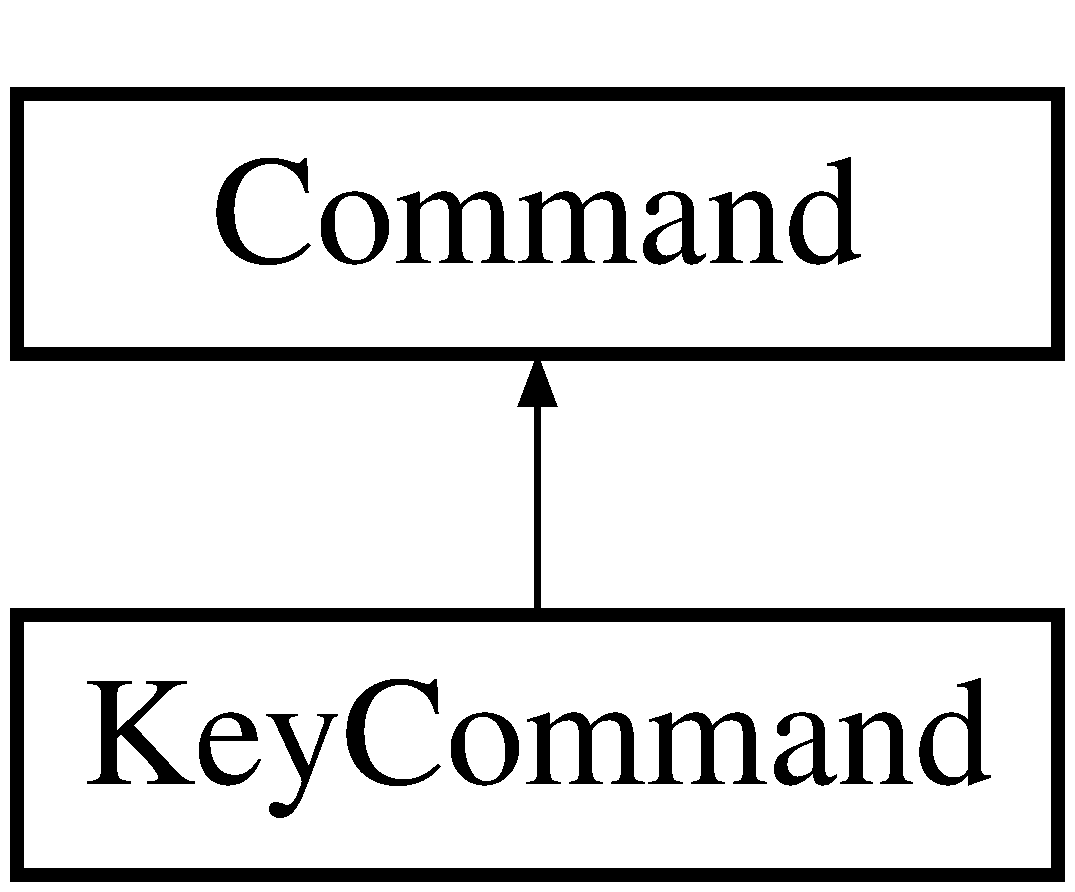
\includegraphics[height=2.000000cm]{class_command}
\end{center}
\end{figure}
\subsection*{Public Types}
\begin{DoxyCompactItemize}
\item 
\mbox{\Hypertarget{class_command_a45bbda49e9ee96d262ac651fefffe487}\label{class_command_a45bbda49e9ee96d262ac651fefffe487}} 
enum \mbox{\hyperlink{class_command_a45bbda49e9ee96d262ac651fefffe487}{Action}} \{ \newline
{\bfseries k\+Invalid}, 
{\bfseries k\+Move\+Up}, 
{\bfseries k\+Move\+Down}, 
{\bfseries k\+Move\+Right}, 
\newline
{\bfseries k\+Move\+Left}, 
{\bfseries k\+Select}, 
{\bfseries k\+Back}, 
{\bfseries k\+Num\+Of\+Actions}
 \}
\begin{DoxyCompactList}\small\item\em Different kinds of actions commands can represent. \end{DoxyCompactList}\item 
\mbox{\Hypertarget{class_command_a4ca33b8d40e12deca5e7bb4190426ee1}\label{class_command_a4ca33b8d40e12deca5e7bb4190426ee1}} 
enum \mbox{\hyperlink{class_command_a4ca33b8d40e12deca5e7bb4190426ee1}{Type}} \{ {\bfseries k\+Invalid}, 
{\bfseries k\+Key}, 
{\bfseries k\+Num\+Of\+Types}
 \}
\begin{DoxyCompactList}\small\item\em Different types of commands can represent. \end{DoxyCompactList}\end{DoxyCompactItemize}
\subsection*{Public Member Functions}
\begin{DoxyCompactItemize}
\item 
\mbox{\hyperlink{class_command_aa511383ade72a941cb61c8498bdf1807}{Command}} (\mbox{\hyperlink{class_command_a45bbda49e9ee96d262ac651fefffe487}{Action}} action=Action\+::k\+Invalid, \mbox{\hyperlink{class_command_a4ca33b8d40e12deca5e7bb4190426ee1}{Type}} type=Type\+::k\+Invalid)
\item 
\mbox{\Hypertarget{class_command_a09802e64142f3c825555b6e77252974e}\label{class_command_a09802e64142f3c825555b6e77252974e}} 
\mbox{\hyperlink{class_command_a45bbda49e9ee96d262ac651fefffe487}{Action}} \mbox{\hyperlink{class_command_a09802e64142f3c825555b6e77252974e}{Get\+Action}} ()
\begin{DoxyCompactList}\small\item\em Returns the action. \end{DoxyCompactList}\end{DoxyCompactItemize}
\subsection*{Protected Attributes}
\begin{DoxyCompactItemize}
\item 
\mbox{\Hypertarget{class_command_aa4b7374825c05006b00ca76c9ed5a021}\label{class_command_aa4b7374825c05006b00ca76c9ed5a021}} 
\mbox{\hyperlink{class_command_a4ca33b8d40e12deca5e7bb4190426ee1}{Type}} \mbox{\hyperlink{class_command_aa4b7374825c05006b00ca76c9ed5a021}{m\+\_\+type}}
\begin{DoxyCompactList}\small\item\em The type. \end{DoxyCompactList}\end{DoxyCompactItemize}


\subsection{Detailed Description}
Interpreted input data and base class for Commands. 

\subsection{Constructor \& Destructor Documentation}
\mbox{\Hypertarget{class_command_aa511383ade72a941cb61c8498bdf1807}\label{class_command_aa511383ade72a941cb61c8498bdf1807}} 
\index{Command@{Command}!Command@{Command}}
\index{Command@{Command}!Command@{Command}}
\subsubsection{\texorpdfstring{Command()}{Command()}}
{\footnotesize\ttfamily Command\+::\+Command (\begin{DoxyParamCaption}\item[{\mbox{\hyperlink{class_command_a45bbda49e9ee96d262ac651fefffe487}{Action}}}]{action = {\ttfamily Action\+:\+:kInvalid},  }\item[{\mbox{\hyperlink{class_command_a4ca33b8d40e12deca5e7bb4190426ee1}{Type}}}]{type = {\ttfamily Type\+:\+:kInvalid} }\end{DoxyParamCaption})}

Constructor 
\begin{DoxyParams}{Parameters}
{\em action} & The command action \\
\hline
{\em type} & The command type \\
\hline
\end{DoxyParams}


The documentation for this class was generated from the following files\+:\begin{DoxyCompactItemize}
\item 
Source/\+Logic/\+Input/\mbox{\hyperlink{_command_8h}{Command.\+h}}\item 
Source/\+Logic/\+Input/Command.\+cpp\end{DoxyCompactItemize}

\hypertarget{class_component_pool}{}\section{Component\+Pool Class Reference}
\label{class_component_pool}\index{Component\+Pool@{Component\+Pool}}


Pool of I\+Components.  




{\ttfamily \#include $<$Component\+Pool.\+h$>$}

\subsection*{Public Types}
\begin{DoxyCompactItemize}
\item 
\mbox{\Hypertarget{class_component_pool_a7a88ce8bc60d1936539c2b9757b7e9ff}\label{class_component_pool_a7a88ce8bc60d1936539c2b9757b7e9ff}} 
enum \mbox{\hyperlink{class_component_pool_a7a88ce8bc60d1936539c2b9757b7e9ff}{Type}} \{ {\bfseries k\+Move}, 
{\bfseries k\+Texture}, 
{\bfseries k\+Physics}, 
{\bfseries k\+Num\+Of\+Compnent\+Types}
 \}
\begin{DoxyCompactList}\small\item\em Component types. \end{DoxyCompactList}\end{DoxyCompactItemize}
\subsection*{Public Member Functions}
\begin{DoxyCompactItemize}
\item 
\mbox{\hyperlink{class_i_component}{I\+Component}} $\ast$ \mbox{\hyperlink{class_component_pool_a08fcae7465ae05cae03872bcaa30203d}{Create\+Component}} (const \mbox{\hyperlink{class_component_pool_a7a88ce8bc60d1936539c2b9757b7e9ff}{Type}} \&type)
\begin{DoxyCompactList}\small\item\em Creates an \mbox{\hyperlink{class_i_component}{I\+Component}} and returns a pointer to it. \end{DoxyCompactList}\item 
void \mbox{\hyperlink{class_component_pool_a5ffc15d4dabb968b528c349aea7b0357}{Delete\+Component}} (unsigned int component\+ID)
\begin{DoxyCompactList}\small\item\em Deletes an \mbox{\hyperlink{class_i_component}{I\+Component}} from the pool. \end{DoxyCompactList}\item 
\mbox{\Hypertarget{class_component_pool_a2744a9ff52ecf322e5a76c4722d7f626}\label{class_component_pool_a2744a9ff52ecf322e5a76c4722d7f626}} 
bool \mbox{\hyperlink{class_component_pool_a2744a9ff52ecf322e5a76c4722d7f626}{Init}} ()
\begin{DoxyCompactList}\small\item\em Initializes the pool. \end{DoxyCompactList}\end{DoxyCompactItemize}


\subsection{Detailed Description}
Pool of I\+Components. 

\subsection{Member Function Documentation}
\mbox{\Hypertarget{class_component_pool_a08fcae7465ae05cae03872bcaa30203d}\label{class_component_pool_a08fcae7465ae05cae03872bcaa30203d}} 
\index{Component\+Pool@{Component\+Pool}!Create\+Component@{Create\+Component}}
\index{Create\+Component@{Create\+Component}!Component\+Pool@{Component\+Pool}}
\subsubsection{\texorpdfstring{Create\+Component()}{CreateComponent()}}
{\footnotesize\ttfamily \mbox{\hyperlink{class_i_component}{I\+Component}} $\ast$ Component\+Pool\+::\+Create\+Component (\begin{DoxyParamCaption}\item[{const \mbox{\hyperlink{class_component_pool_a7a88ce8bc60d1936539c2b9757b7e9ff}{Type}} \&}]{type }\end{DoxyParamCaption})}



Creates an \mbox{\hyperlink{class_i_component}{I\+Component}} and returns a pointer to it. 


\begin{DoxyParams}{Parameters}
{\em type} & Type of component to be created. \\
\hline
\end{DoxyParams}
\mbox{\Hypertarget{class_component_pool_a5ffc15d4dabb968b528c349aea7b0357}\label{class_component_pool_a5ffc15d4dabb968b528c349aea7b0357}} 
\index{Component\+Pool@{Component\+Pool}!Delete\+Component@{Delete\+Component}}
\index{Delete\+Component@{Delete\+Component}!Component\+Pool@{Component\+Pool}}
\subsubsection{\texorpdfstring{Delete\+Component()}{DeleteComponent()}}
{\footnotesize\ttfamily void Component\+Pool\+::\+Delete\+Component (\begin{DoxyParamCaption}\item[{unsigned int}]{component\+ID }\end{DoxyParamCaption})}



Deletes an \mbox{\hyperlink{class_i_component}{I\+Component}} from the pool. 


\begin{DoxyParams}{Parameters}
{\em component\+ID} & ID of the component to delete. \\
\hline
\end{DoxyParams}


The documentation for this class was generated from the following files\+:\begin{DoxyCompactItemize}
\item 
Source/\+Logic/\+Game\+Objects/\mbox{\hyperlink{_component_pool_8h}{Component\+Pool.\+h}}\item 
Source/\+Logic/\+Game\+Objects/Component\+Pool.\+cpp\end{DoxyCompactItemize}

\hypertarget{classtinyxml2_1_1_dyn_array}{}\section{tinyxml2\+:\+:Dyn\+Array$<$ T, I\+N\+I\+T\+I\+A\+L\+\_\+\+S\+I\+ZE $>$ Class Template Reference}
\label{classtinyxml2_1_1_dyn_array}\index{tinyxml2\+::\+Dyn\+Array$<$ T, I\+N\+I\+T\+I\+A\+L\+\_\+\+S\+I\+Z\+E $>$@{tinyxml2\+::\+Dyn\+Array$<$ T, I\+N\+I\+T\+I\+A\+L\+\_\+\+S\+I\+Z\+E $>$}}
\subsection*{Public Member Functions}
\begin{DoxyCompactItemize}
\item 
\mbox{\Hypertarget{classtinyxml2_1_1_dyn_array_af87a804cd831226d069274b44b74b8bc}\label{classtinyxml2_1_1_dyn_array_af87a804cd831226d069274b44b74b8bc}} 
void {\bfseries Clear} ()
\item 
\mbox{\Hypertarget{classtinyxml2_1_1_dyn_array_aea7ffe983b5d3284bd43171afd7c99d0}\label{classtinyxml2_1_1_dyn_array_aea7ffe983b5d3284bd43171afd7c99d0}} 
void {\bfseries Push} (T t)
\item 
\mbox{\Hypertarget{classtinyxml2_1_1_dyn_array_ad289abee8cd02b26e215f1b63d2043f1}\label{classtinyxml2_1_1_dyn_array_ad289abee8cd02b26e215f1b63d2043f1}} 
T $\ast$ {\bfseries Push\+Arr} (int count)
\item 
\mbox{\Hypertarget{classtinyxml2_1_1_dyn_array_a27a3f2f6f869815b6eabb3ea40cf0712}\label{classtinyxml2_1_1_dyn_array_a27a3f2f6f869815b6eabb3ea40cf0712}} 
T {\bfseries Pop} ()
\item 
\mbox{\Hypertarget{classtinyxml2_1_1_dyn_array_ab8b8c94a2312ab27e2846f0d61ef677a}\label{classtinyxml2_1_1_dyn_array_ab8b8c94a2312ab27e2846f0d61ef677a}} 
void {\bfseries Pop\+Arr} (int count)
\item 
\mbox{\Hypertarget{classtinyxml2_1_1_dyn_array_a044fc26f44ed3e96ffaeac542188149e}\label{classtinyxml2_1_1_dyn_array_a044fc26f44ed3e96ffaeac542188149e}} 
bool {\bfseries Empty} () const
\item 
\mbox{\Hypertarget{classtinyxml2_1_1_dyn_array_a756cf4e7464c711aa720e2b17a251daa}\label{classtinyxml2_1_1_dyn_array_a756cf4e7464c711aa720e2b17a251daa}} 
T \& {\bfseries operator\mbox{[}$\,$\mbox{]}} (int i)
\item 
\mbox{\Hypertarget{classtinyxml2_1_1_dyn_array_a474a5cd9bc97ea32b3dcef4c773125e1}\label{classtinyxml2_1_1_dyn_array_a474a5cd9bc97ea32b3dcef4c773125e1}} 
const T \& {\bfseries operator\mbox{[}$\,$\mbox{]}} (int i) const
\item 
\mbox{\Hypertarget{classtinyxml2_1_1_dyn_array_a5e4e1e408e646688503dec77c77c9d59}\label{classtinyxml2_1_1_dyn_array_a5e4e1e408e646688503dec77c77c9d59}} 
const T \& {\bfseries Peek\+Top} () const
\item 
\mbox{\Hypertarget{classtinyxml2_1_1_dyn_array_a67614d80847eb92cab330f1a5849a9a2}\label{classtinyxml2_1_1_dyn_array_a67614d80847eb92cab330f1a5849a9a2}} 
int {\bfseries Size} () const
\item 
\mbox{\Hypertarget{classtinyxml2_1_1_dyn_array_a8e101fdf5b4248ac119d7dca6d0f5421}\label{classtinyxml2_1_1_dyn_array_a8e101fdf5b4248ac119d7dca6d0f5421}} 
int {\bfseries Capacity} () const
\item 
\mbox{\Hypertarget{classtinyxml2_1_1_dyn_array_aa72c644f8b5e9ec5dab5b66c88f5665f}\label{classtinyxml2_1_1_dyn_array_aa72c644f8b5e9ec5dab5b66c88f5665f}} 
void {\bfseries Swap\+Remove} (int i)
\item 
\mbox{\Hypertarget{classtinyxml2_1_1_dyn_array_a60b33e61cf10b3fd900ee46692dc0fe9}\label{classtinyxml2_1_1_dyn_array_a60b33e61cf10b3fd900ee46692dc0fe9}} 
const T $\ast$ {\bfseries Mem} () const
\item 
\mbox{\Hypertarget{classtinyxml2_1_1_dyn_array_a2f0842cd666e2ad951f1a8bd6561fa40}\label{classtinyxml2_1_1_dyn_array_a2f0842cd666e2ad951f1a8bd6561fa40}} 
T $\ast$ {\bfseries Mem} ()
\end{DoxyCompactItemize}


The documentation for this class was generated from the following file\+:\begin{DoxyCompactItemize}
\item 
Source/\+Utils/tinyxml2.\+h\end{DoxyCompactItemize}

\hypertarget{structtinyxml2_1_1_entity}{}\section{tinyxml2\+:\+:Entity Struct Reference}
\label{structtinyxml2_1_1_entity}\index{tinyxml2\+::\+Entity@{tinyxml2\+::\+Entity}}
\subsection*{Public Attributes}
\begin{DoxyCompactItemize}
\item 
\mbox{\Hypertarget{structtinyxml2_1_1_entity_ab330f5d665d29bfc811ecfa76315894b}\label{structtinyxml2_1_1_entity_ab330f5d665d29bfc811ecfa76315894b}} 
const char $\ast$ {\bfseries pattern}
\item 
\mbox{\Hypertarget{structtinyxml2_1_1_entity_a25e2b57cb59cb4fa68f283d7cb570f21}\label{structtinyxml2_1_1_entity_a25e2b57cb59cb4fa68f283d7cb570f21}} 
int {\bfseries length}
\item 
\mbox{\Hypertarget{structtinyxml2_1_1_entity_a7334e81e33b4615655a403711b24f3ed}\label{structtinyxml2_1_1_entity_a7334e81e33b4615655a403711b24f3ed}} 
char {\bfseries value}
\end{DoxyCompactItemize}


The documentation for this struct was generated from the following file\+:\begin{DoxyCompactItemize}
\item 
Source/\+Utils/tinyxml2.\+cpp\end{DoxyCompactItemize}

\hypertarget{struct_event}{}\section{Event Struct Reference}
\label{struct_event}\index{Event@{Event}}


\mbox{\hyperlink{struct_event}{Event}} structure.  




{\ttfamily \#include $<$Event\+System.\+h$>$}

Inheritance diagram for Event\+:\begin{figure}[H]
\begin{center}
\leavevmode
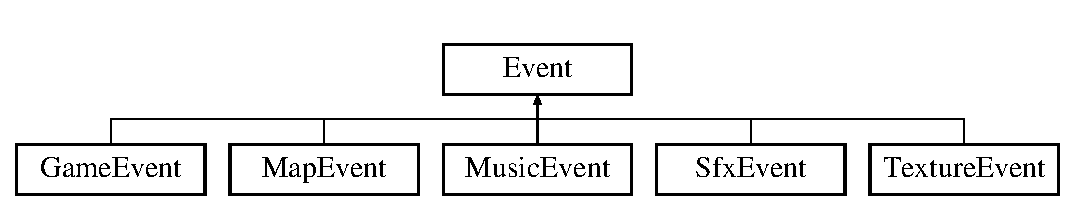
\includegraphics[height=2.000000cm]{struct_event}
\end{center}
\end{figure}
\subsection*{Public Types}
\begin{DoxyCompactItemize}
\item 
\mbox{\Hypertarget{struct_event_a2abf13b5be49315e9e362af02029f058}\label{struct_event_a2abf13b5be49315e9e362af02029f058}} 
enum {\bfseries Type} \{ \newline
{\bfseries k\+Game}, 
{\bfseries k\+Map}, 
{\bfseries k\+View}, 
{\bfseries k\+Load\+Sfx}, 
\newline
{\bfseries k\+Play\+Sfx}, 
{\bfseries k\+Load\+Music}, 
{\bfseries k\+Play\+Music}, 
{\bfseries k\+Load\+Texture}, 
\newline
{\bfseries k\+Request\+Texture}, 
{\bfseries k\+Send\+Texture}, 
{\bfseries k\+Num\+Of\+Types}
 \}
\end{DoxyCompactItemize}
\subsection*{Public Attributes}
\begin{DoxyCompactItemize}
\item 
\mbox{\Hypertarget{struct_event_a4b6df7508772bf848466b71623666c97}\label{struct_event_a4b6df7508772bf848466b71623666c97}} 
Type \mbox{\hyperlink{struct_event_a4b6df7508772bf848466b71623666c97}{m\+\_\+type}}
\begin{DoxyCompactList}\small\item\em Type of event. \end{DoxyCompactList}\item 
\mbox{\Hypertarget{struct_event_aa5135558b0fd21b4c385bdc01522cebf}\label{struct_event_aa5135558b0fd21b4c385bdc01522cebf}} 
std\+::string \mbox{\hyperlink{struct_event_aa5135558b0fd21b4c385bdc01522cebf}{m\+\_\+event\+Str}}
\begin{DoxyCompactList}\small\item\em T\+E\+ST\+: only here to test sending and recieving of events. \end{DoxyCompactList}\end{DoxyCompactItemize}


\subsection{Detailed Description}
\mbox{\hyperlink{struct_event}{Event}} structure. 

The documentation for this struct was generated from the following file\+:\begin{DoxyCompactItemize}
\item 
Source/\+Logic/\+Events/\mbox{\hyperlink{_event_system_8h}{Event\+System.\+h}}\end{DoxyCompactItemize}

\hypertarget{class_event_system}{}\section{Event\+System Class Reference}
\label{class_event_system}\index{Event\+System@{Event\+System}}


System to handle sending and recieving of Events.  




{\ttfamily \#include $<$Event\+System.\+h$>$}

\subsection*{Public Member Functions}
\begin{DoxyCompactItemize}
\item 
\mbox{\hyperlink{class_event_system_a461a525365e056375c1e4177897688ed}{Event\+System}} ()=delete
\end{DoxyCompactItemize}
\subsection*{Static Public Member Functions}
\begin{DoxyCompactItemize}
\item 
static void \mbox{\hyperlink{class_event_system_a25048a2cae1066f84ce0e0c7aecf6314}{Subscribe\+Handler}} (const Event\+::\+Type \&event\+Type, \mbox{\hyperlink{class_i_event_handler}{I\+Event\+Handler}} $\ast$p\+Handler)
\begin{DoxyCompactList}\small\item\em Subscribes a handler to an event. \end{DoxyCompactList}\item 
static void \mbox{\hyperlink{class_event_system_ae8ebabb2d7e4604b3d5f666d9bcb1d32}{Unsubscribe\+Handler}} (const Event\+::\+Type \&event\+Type, \mbox{\hyperlink{class_i_event_handler}{I\+Event\+Handler}} $\ast$p\+Handler)
\begin{DoxyCompactList}\small\item\em Unsubscribes a handler from an event. \end{DoxyCompactList}\item 
static void \mbox{\hyperlink{class_event_system_ae7f287c5ee2c8001e19467ae8fda8a67}{Broadcast\+Event}} (\mbox{\hyperlink{struct_event}{Event}} $\ast$p\+Event)
\begin{DoxyCompactList}\small\item\em Broadcasts an event to all its handlers. \end{DoxyCompactList}\end{DoxyCompactItemize}


\subsection{Detailed Description}
System to handle sending and recieving of Events. 

\subsection{Constructor \& Destructor Documentation}
\mbox{\Hypertarget{class_event_system_a461a525365e056375c1e4177897688ed}\label{class_event_system_a461a525365e056375c1e4177897688ed}} 
\index{Event\+System@{Event\+System}!Event\+System@{Event\+System}}
\index{Event\+System@{Event\+System}!Event\+System@{Event\+System}}
\subsubsection{\texorpdfstring{Event\+System()}{EventSystem()}}
{\footnotesize\ttfamily Event\+System\+::\+Event\+System (\begin{DoxyParamCaption}{ }\end{DoxyParamCaption})\hspace{0.3cm}{\ttfamily [delete]}}

Constructor Not ment to be invoked 

\subsection{Member Function Documentation}
\mbox{\Hypertarget{class_event_system_ae7f287c5ee2c8001e19467ae8fda8a67}\label{class_event_system_ae7f287c5ee2c8001e19467ae8fda8a67}} 
\index{Event\+System@{Event\+System}!Broadcast\+Event@{Broadcast\+Event}}
\index{Broadcast\+Event@{Broadcast\+Event}!Event\+System@{Event\+System}}
\subsubsection{\texorpdfstring{Broadcast\+Event()}{BroadcastEvent()}}
{\footnotesize\ttfamily void Event\+System\+::\+Broadcast\+Event (\begin{DoxyParamCaption}\item[{\mbox{\hyperlink{struct_event}{Event}} $\ast$}]{p\+Event }\end{DoxyParamCaption})\hspace{0.3cm}{\ttfamily [static]}}



Broadcasts an event to all its handlers. 


\begin{DoxyParams}{Parameters}
{\em p\+Event} & pointer to \mbox{\hyperlink{struct_event}{Event}} to broadcast \\
\hline
\end{DoxyParams}
\mbox{\Hypertarget{class_event_system_a25048a2cae1066f84ce0e0c7aecf6314}\label{class_event_system_a25048a2cae1066f84ce0e0c7aecf6314}} 
\index{Event\+System@{Event\+System}!Subscribe\+Handler@{Subscribe\+Handler}}
\index{Subscribe\+Handler@{Subscribe\+Handler}!Event\+System@{Event\+System}}
\subsubsection{\texorpdfstring{Subscribe\+Handler()}{SubscribeHandler()}}
{\footnotesize\ttfamily void Event\+System\+::\+Subscribe\+Handler (\begin{DoxyParamCaption}\item[{const Event\+::\+Type \&}]{event\+Type,  }\item[{\mbox{\hyperlink{class_i_event_handler}{I\+Event\+Handler}} $\ast$}]{p\+Handler }\end{DoxyParamCaption})\hspace{0.3cm}{\ttfamily [static]}}



Subscribes a handler to an event. 


\begin{DoxyParams}{Parameters}
{\em event\+Type} & The type of event to subscribe the handler to \\
\hline
{\em p\+Handler} & pointer to the handler that will be subscribed \\
\hline
\end{DoxyParams}
\mbox{\Hypertarget{class_event_system_ae8ebabb2d7e4604b3d5f666d9bcb1d32}\label{class_event_system_ae8ebabb2d7e4604b3d5f666d9bcb1d32}} 
\index{Event\+System@{Event\+System}!Unsubscribe\+Handler@{Unsubscribe\+Handler}}
\index{Unsubscribe\+Handler@{Unsubscribe\+Handler}!Event\+System@{Event\+System}}
\subsubsection{\texorpdfstring{Unsubscribe\+Handler()}{UnsubscribeHandler()}}
{\footnotesize\ttfamily void Event\+System\+::\+Unsubscribe\+Handler (\begin{DoxyParamCaption}\item[{const Event\+::\+Type \&}]{event\+Type,  }\item[{\mbox{\hyperlink{class_i_event_handler}{I\+Event\+Handler}} $\ast$}]{p\+Handler }\end{DoxyParamCaption})\hspace{0.3cm}{\ttfamily [static]}}



Unsubscribes a handler from an event. 


\begin{DoxyParams}{Parameters}
{\em event\+Type} & The type of event to unsubscribe the handler from \\
\hline
{\em p\+Handler} & pointer to the handler that will be unsubscribed \\
\hline
\end{DoxyParams}


The documentation for this class was generated from the following files\+:\begin{DoxyCompactItemize}
\item 
Source/\+Logic/\+Events/\mbox{\hyperlink{_event_system_8h}{Event\+System.\+h}}\item 
Source/\+Logic/\+Events/Event\+System.\+cpp\end{DoxyCompactItemize}

\hypertarget{class_game}{}\section{Game Class Reference}
\label{class_game}\index{Game@{Game}}


Represents game logic.  




{\ttfamily \#include $<$Game.\+h$>$}

Inheritance diagram for Game\+:\begin{figure}[H]
\begin{center}
\leavevmode
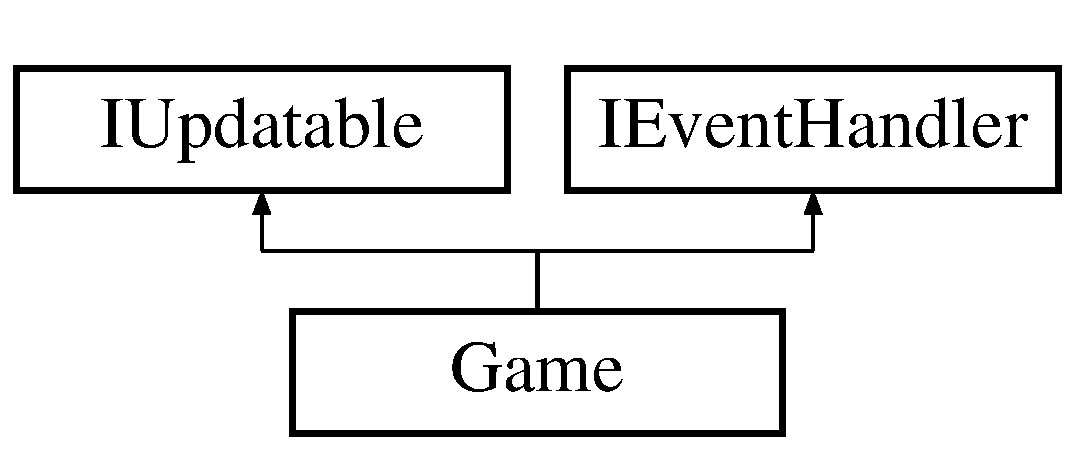
\includegraphics[height=2.000000cm]{class_game}
\end{center}
\end{figure}
\subsection*{Public Member Functions}
\begin{DoxyCompactItemize}
\item 
bool \mbox{\hyperlink{class_game_a083fc4d208482811d5dd6efb5c7fbaf4}{Init}} (\mbox{\hyperlink{class_object_pool}{Object\+Pool}} $\ast$p\+Obj\+Pool, \mbox{\hyperlink{class_component_pool}{Component\+Pool}} $\ast$p\+Component\+Pool, lua\+\_\+\+State $\ast$p\+Lua\+State)
\begin{DoxyCompactList}\small\item\em Initializes the game. \end{DoxyCompactList}\item 
\mbox{\Hypertarget{class_game_afe8f2a4980f240bbfba8c1f495ff5075}\label{class_game_afe8f2a4980f240bbfba8c1f495ff5075}} 
void \mbox{\hyperlink{class_game_afe8f2a4980f240bbfba8c1f495ff5075}{Clean\+Up}} ()
\begin{DoxyCompactList}\small\item\em Cleans up game from memory. \end{DoxyCompactList}\item 
virtual \mbox{\hyperlink{_macros_8h_a9ce0e6835f82908079752fa4ebe70dc9}{P\+H\+A\+Z\+E\+\_\+\+A\+PI}} void \mbox{\hyperlink{class_game_a49cc5bc8eee98577d72cd49dfc3c4af5}{Update}} (const float delta\+Time\+\_\+sec) override
\begin{DoxyCompactList}\small\item\em Updates the game. \end{DoxyCompactList}\item 
\mbox{\Hypertarget{class_game_a622f72b9b81370d4d77f7b625a36fd75}\label{class_game_a622f72b9b81370d4d77f7b625a36fd75}} 
void \mbox{\hyperlink{class_game_a622f72b9b81370d4d77f7b625a36fd75}{Handle\+Key\+Command}} (\mbox{\hyperlink{class_key_command}{Key\+Command}} \&key\+Command)
\begin{DoxyCompactList}\small\item\em Handles a key command. \end{DoxyCompactList}\item 
\mbox{\Hypertarget{class_game_a379673c1cde729d801e6f14f7b394810}\label{class_game_a379673c1cde729d801e6f14f7b394810}} 
virtual \mbox{\hyperlink{_macros_8h_a9ce0e6835f82908079752fa4ebe70dc9}{P\+H\+A\+Z\+E\+\_\+\+A\+PI}} void \mbox{\hyperlink{class_game_a379673c1cde729d801e6f14f7b394810}{Handle\+Event}} (\mbox{\hyperlink{struct_event}{Event}} $\ast$p\+Event) override
\begin{DoxyCompactList}\small\item\em Hanldes an event. \end{DoxyCompactList}\item 
\mbox{\Hypertarget{class_game_a00a6ce87351c9bc799834b0061396bbd}\label{class_game_a00a6ce87351c9bc799834b0061396bbd}} 
bool \mbox{\hyperlink{class_game_a00a6ce87351c9bc799834b0061396bbd}{Get\+Playing\+Flag}} ()
\begin{DoxyCompactList}\small\item\em Returns playing flag. \end{DoxyCompactList}\item 
\mbox{\Hypertarget{class_game_a69ee850fc9c3af5373a60ea26c2e6700}\label{class_game_a69ee850fc9c3af5373a60ea26c2e6700}} 
void \mbox{\hyperlink{class_game_a69ee850fc9c3af5373a60ea26c2e6700}{Quit\+Game}} ()
\begin{DoxyCompactList}\small\item\em Sets playing flag to false. \end{DoxyCompactList}\item 
std\+::vector$<$ \mbox{\hyperlink{class_game_object}{Game\+Object}} $\ast$ $>$ $\ast$ \mbox{\hyperlink{class_game_af132c9a360c2adafd158c3a331b39c4d}{Get\+Game\+Objects}} ()
\begin{DoxyCompactList}\small\item\em Returns test game object. \end{DoxyCompactList}\end{DoxyCompactItemize}


\subsection{Detailed Description}
Represents game logic. 

\subsection{Member Function Documentation}
\mbox{\Hypertarget{class_game_af132c9a360c2adafd158c3a331b39c4d}\label{class_game_af132c9a360c2adafd158c3a331b39c4d}} 
\index{Game@{Game}!Get\+Game\+Objects@{Get\+Game\+Objects}}
\index{Get\+Game\+Objects@{Get\+Game\+Objects}!Game@{Game}}
\subsubsection{\texorpdfstring{Get\+Game\+Objects()}{GetGameObjects()}}
{\footnotesize\ttfamily std\+::vector$<$\mbox{\hyperlink{class_game_object}{Game\+Object}}$\ast$$>$$\ast$ Game\+::\+Get\+Game\+Objects (\begin{DoxyParamCaption}{ }\end{DoxyParamCaption})\hspace{0.3cm}{\ttfamily [inline]}}



Returns test game object. 

Returns a pointer to the list of Game\+Objects \mbox{\Hypertarget{class_game_a083fc4d208482811d5dd6efb5c7fbaf4}\label{class_game_a083fc4d208482811d5dd6efb5c7fbaf4}} 
\index{Game@{Game}!Init@{Init}}
\index{Init@{Init}!Game@{Game}}
\subsubsection{\texorpdfstring{Init()}{Init()}}
{\footnotesize\ttfamily bool Game\+::\+Init (\begin{DoxyParamCaption}\item[{\mbox{\hyperlink{class_object_pool}{Object\+Pool}} $\ast$}]{p\+Obj\+Pool,  }\item[{\mbox{\hyperlink{class_component_pool}{Component\+Pool}} $\ast$}]{p\+Component\+Pool,  }\item[{lua\+\_\+\+State $\ast$}]{p\+Lua\+State }\end{DoxyParamCaption})}



Initializes the game. 


\begin{DoxyParams}{Parameters}
{\em p\+View} & \mbox{\hyperlink{class_view}{View}} delegate \\
\hline
\end{DoxyParams}
\mbox{\Hypertarget{class_game_a49cc5bc8eee98577d72cd49dfc3c4af5}\label{class_game_a49cc5bc8eee98577d72cd49dfc3c4af5}} 
\index{Game@{Game}!Update@{Update}}
\index{Update@{Update}!Game@{Game}}
\subsubsection{\texorpdfstring{Update()}{Update()}}
{\footnotesize\ttfamily void Game\+::\+Update (\begin{DoxyParamCaption}\item[{const float}]{delta\+Time\+\_\+sec }\end{DoxyParamCaption})\hspace{0.3cm}{\ttfamily [override]}, {\ttfamily [virtual]}}



Updates the game. 


\begin{DoxyParams}{Parameters}
{\em delta\+Time\+\_\+sec} & Time since last frame in seconds \\
\hline
\end{DoxyParams}


Implements \mbox{\hyperlink{class_i_updatable_a291a40a3422a0b02ef4c10e1d1570eb0}{I\+Updatable}}.



The documentation for this class was generated from the following files\+:\begin{DoxyCompactItemize}
\item 
Source/\+Logic/\mbox{\hyperlink{_game_8h}{Game.\+h}}\item 
Source/\+Logic/Game.\+cpp\end{DoxyCompactItemize}

\hypertarget{struct_game_event}{}\section{Game\+Event Struct Reference}
\label{struct_game_event}\index{Game\+Event@{Game\+Event}}


Structure for \mbox{\hyperlink{class_game}{Game}} Logic Events.  




{\ttfamily \#include $<$Event\+System.\+h$>$}

Inheritance diagram for Game\+Event\+:\begin{figure}[H]
\begin{center}
\leavevmode
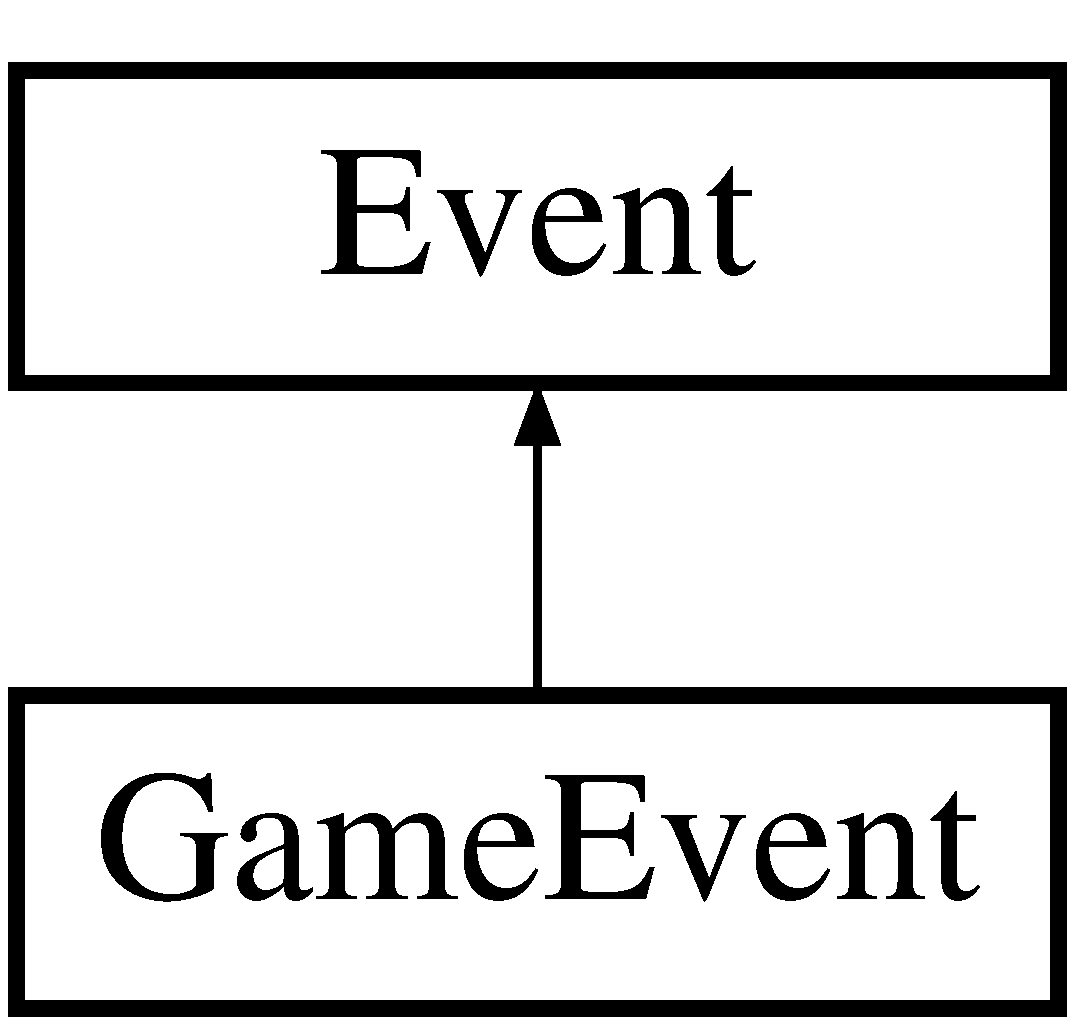
\includegraphics[height=2.000000cm]{struct_game_event}
\end{center}
\end{figure}
\subsection*{Public Attributes}
\begin{DoxyCompactItemize}
\item 
\mbox{\Hypertarget{struct_game_event_a1ee24a4ec74cbe87a4b1eb634000a324}\label{struct_game_event_a1ee24a4ec74cbe87a4b1eb634000a324}} 
std\+::vector$<$ \mbox{\hyperlink{class_game_object}{Game\+Object}} $\ast$ $>$ $\ast$ \mbox{\hyperlink{struct_game_event_a1ee24a4ec74cbe87a4b1eb634000a324}{m\+\_\+p\+Game\+Objects}}
\begin{DoxyCompactList}\small\item\em List of this event\textquotesingle{}s game objects. \end{DoxyCompactList}\end{DoxyCompactItemize}
\subsection*{Additional Inherited Members}


\subsection{Detailed Description}
Structure for \mbox{\hyperlink{class_game}{Game}} Logic Events. 

The documentation for this struct was generated from the following file\+:\begin{DoxyCompactItemize}
\item 
Source/\+Logic/\+Events/\mbox{\hyperlink{_event_system_8h}{Event\+System.\+h}}\end{DoxyCompactItemize}

\hypertarget{class_game_object}{}\section{Game\+Object Class Reference}
\label{class_game_object}\index{Game\+Object@{Game\+Object}}


Represents a game object.  




{\ttfamily \#include $<$Game\+Object.\+h$>$}

Inheritance diagram for Game\+Object\+:\begin{figure}[H]
\begin{center}
\leavevmode
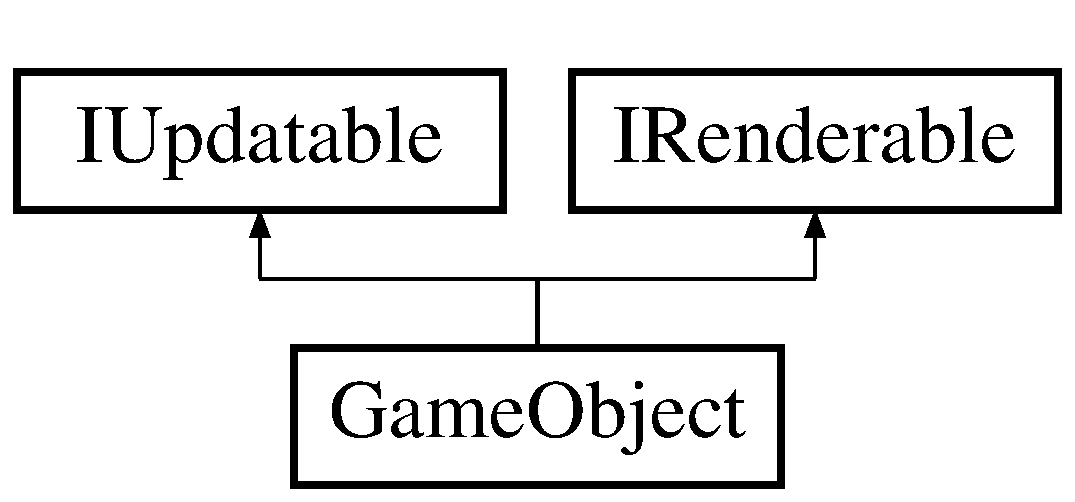
\includegraphics[height=2.000000cm]{class_game_object}
\end{center}
\end{figure}
\subsection*{Public Member Functions}
\begin{DoxyCompactItemize}
\item 
\mbox{\Hypertarget{class_game_object_a0348e3ee2e83d56eafca7a3547f432c4}\label{class_game_object_a0348e3ee2e83d56eafca7a3547f432c4}} 
\mbox{\hyperlink{class_game_object_a0348e3ee2e83d56eafca7a3547f432c4}{Game\+Object}} ()
\begin{DoxyCompactList}\small\item\em Default Constructor. \end{DoxyCompactList}\item 
\mbox{\hyperlink{class_game_object_a0cefa9305b62d18a11d7c1182fcbf5bc}{Game\+Object}} (const \mbox{\hyperlink{class_game_object}{Game\+Object}} \&original)
\begin{DoxyCompactList}\small\item\em Copy Constructor. \end{DoxyCompactList}\item 
virtual \mbox{\hyperlink{_macros_8h_a9ce0e6835f82908079752fa4ebe70dc9}{P\+H\+A\+Z\+E\+\_\+\+A\+PI}} void \mbox{\hyperlink{class_game_object_a931541422ec57567e1d46436d97b874c}{Update}} (float delta\+Time\+\_\+sec) override
\begin{DoxyCompactList}\small\item\em Updates the game object. \end{DoxyCompactList}\item 
\mbox{\Hypertarget{class_game_object_af9450b108e616d4e30c7a88534517df0}\label{class_game_object_af9450b108e616d4e30c7a88534517df0}} 
virtual \mbox{\hyperlink{_macros_8h_a9ce0e6835f82908079752fa4ebe70dc9}{P\+H\+A\+Z\+E\+\_\+\+A\+PI}} void \mbox{\hyperlink{class_game_object_af9450b108e616d4e30c7a88534517df0}{Render}} () override
\begin{DoxyCompactList}\small\item\em Renders the game object. \end{DoxyCompactList}\item 
void \mbox{\hyperlink{class_game_object_a1e8c34679f8e8decbd9628a890f47c7f}{Attach\+Component}} (const \mbox{\hyperlink{class_component_pool_a7a88ce8bc60d1936539c2b9757b7e9ff}{Component\+Pool\+::\+Type}} \&type)
\begin{DoxyCompactList}\small\item\em Attaches a component to this game object. \end{DoxyCompactList}\item 
void \mbox{\hyperlink{class_game_object_a4d100b6ecc6476f52c72f0889e6c06d4}{Dettach\+Component}} (const unsigned int component\+ID)
\begin{DoxyCompactList}\small\item\em Detaches a component from this game object. \end{DoxyCompactList}\item 
\mbox{\Hypertarget{class_game_object_a44d7b100b46dafcfe895baf15ee39eff}\label{class_game_object_a44d7b100b46dafcfe895baf15ee39eff}} 
\mbox{\hyperlink{struct_vector2_d}{Vector2D}} \mbox{\hyperlink{class_game_object_a44d7b100b46dafcfe895baf15ee39eff}{Get\+Position}} ()
\begin{DoxyCompactList}\small\item\em Returns position. \end{DoxyCompactList}\item 
void \mbox{\hyperlink{class_game_object_a0c213e4df823a0f68cf8906a6937f88e}{Set\+Position}} (\mbox{\hyperlink{struct_vector2_d}{Vector2D}} new\+Pos)
\begin{DoxyCompactList}\small\item\em Sets the position. \end{DoxyCompactList}\item 
\mbox{\Hypertarget{class_game_object_a71e9fe489b7c5ef7e8e0368ec71fac6d}\label{class_game_object_a71e9fe489b7c5ef7e8e0368ec71fac6d}} 
\mbox{\hyperlink{struct_vector2_d}{Vector2D}} \mbox{\hyperlink{class_game_object_a71e9fe489b7c5ef7e8e0368ec71fac6d}{Get\+Size}} ()
\begin{DoxyCompactList}\small\item\em Returns size. \end{DoxyCompactList}\item 
void \mbox{\hyperlink{class_game_object_a67cd10342fab71294976bf7fd5e22e01}{Set\+Size}} (\mbox{\hyperlink{struct_vector2_d}{Vector2D}} new\+Size)
\begin{DoxyCompactList}\small\item\em Sets the size. \end{DoxyCompactList}\item 
\mbox{\Hypertarget{class_game_object_aac34f983d635994932c3b7a5c4e3e49a}\label{class_game_object_aac34f983d635994932c3b7a5c4e3e49a}} 
\mbox{\hyperlink{struct_vector2_d}{Vector2D}} \mbox{\hyperlink{class_game_object_aac34f983d635994932c3b7a5c4e3e49a}{Get\+Move\+Dir}} ()
\begin{DoxyCompactList}\small\item\em Returns movement direction. \end{DoxyCompactList}\item 
void \mbox{\hyperlink{class_game_object_a11c2fa0ca47cbeb27d4887573a913438}{Set\+Move\+Dir}} (\mbox{\hyperlink{struct_vector2_d}{Vector2D}} new\+Dir)
\begin{DoxyCompactList}\small\item\em Sets the movement direction. \end{DoxyCompactList}\item 
\mbox{\Hypertarget{class_game_object_a8dfeba914fba847488d3bff6e068f7a2}\label{class_game_object_a8dfeba914fba847488d3bff6e068f7a2}} 
std\+::string \mbox{\hyperlink{class_game_object_a8dfeba914fba847488d3bff6e068f7a2}{Get\+Obj\+Name}} ()
\begin{DoxyCompactList}\small\item\em Returns object name. \end{DoxyCompactList}\item 
void \mbox{\hyperlink{class_game_object_a400594b6957192dfe9cddaa513f49d7e}{Set\+Obj\+Name}} (std\+::string new\+Name)
\begin{DoxyCompactList}\small\item\em Sets the name. \end{DoxyCompactList}\item 
\mbox{\Hypertarget{class_game_object_a60d86fa7dab47fccf8255760612f6de1}\label{class_game_object_a60d86fa7dab47fccf8255760612f6de1}} 
S\+D\+L\+\_\+\+Rect \mbox{\hyperlink{class_game_object_a60d86fa7dab47fccf8255760612f6de1}{Get\+Obj\+Rect}} ()
\begin{DoxyCompactList}\small\item\em Returns the sdl rect. \end{DoxyCompactList}\item 
void \mbox{\hyperlink{class_game_object_a898813cdba2aa0888f6e5b0e4fc6ac64}{Set\+Obj\+Rect}} (S\+D\+L\+\_\+\+Rect new\+Rect)
\begin{DoxyCompactList}\small\item\em Sets the name. \end{DoxyCompactList}\item 
\mbox{\Hypertarget{class_game_object_a7fcf07003ef5424a7ce46461a8a0be06}\label{class_game_object_a7fcf07003ef5424a7ce46461a8a0be06}} 
\mbox{\hyperlink{struct_texture_component}{Texture\+Component}} $\ast$ \mbox{\hyperlink{class_game_object_a7fcf07003ef5424a7ce46461a8a0be06}{Get\+Texture\+Component}} ()
\begin{DoxyCompactList}\small\item\em Returns the sdl texture. \end{DoxyCompactList}\item 
\mbox{\Hypertarget{class_game_object_a8b709e89ace9675b822b50bdd2ac879d}\label{class_game_object_a8b709e89ace9675b822b50bdd2ac879d}} 
\mbox{\hyperlink{struct_physics_component}{Physics\+Component}} $\ast$ \mbox{\hyperlink{class_game_object_a8b709e89ace9675b822b50bdd2ac879d}{Get\+Physics\+Component}} ()
\begin{DoxyCompactList}\small\item\em Returns the physics component. \end{DoxyCompactList}\item 
void \mbox{\hyperlink{class_game_object_ae232f791564f4bf504e0ede697be7f0d}{Set\+Component\+Pool}} (\mbox{\hyperlink{class_component_pool}{Component\+Pool}} $\ast$p\+New\+Pool)
\begin{DoxyCompactList}\small\item\em Sets the component pool to use. \end{DoxyCompactList}\item 
\mbox{\Hypertarget{class_game_object_acc49d53385a1e3b344d59f177c09d91b}\label{class_game_object_acc49d53385a1e3b344d59f177c09d91b}} 
unsigned int \mbox{\hyperlink{class_game_object_acc49d53385a1e3b344d59f177c09d91b}{Get\+ID}} ()
\begin{DoxyCompactList}\small\item\em Returns Object ID. \end{DoxyCompactList}\item 
\mbox{\Hypertarget{class_game_object_af8b86b903fa6133147beecd900d4cb68}\label{class_game_object_af8b86b903fa6133147beecd900d4cb68}} 
void \mbox{\hyperlink{class_game_object_af8b86b903fa6133147beecd900d4cb68}{Set\+ID}} (unsigned int new\+ID)
\begin{DoxyCompactList}\small\item\em Sets the Object ID. \end{DoxyCompactList}\item 
\mbox{\Hypertarget{class_game_object_aacd344875d0bee0c5a95af28305aa94a}\label{class_game_object_aacd344875d0bee0c5a95af28305aa94a}} 
void \mbox{\hyperlink{class_game_object_aacd344875d0bee0c5a95af28305aa94a}{Attach\+To\+Lua\+Table}} ()
\begin{DoxyCompactList}\small\item\em Attaches the lua state. \end{DoxyCompactList}\item 
\mbox{\Hypertarget{class_game_object_ac01455f6ad0b0b4bc3e6c51c6624fde4}\label{class_game_object_ac01455f6ad0b0b4bc3e6c51c6624fde4}} 
void \mbox{\hyperlink{class_game_object_ac01455f6ad0b0b4bc3e6c51c6624fde4}{Attach\+Lua\+State}} (lua\+\_\+\+State $\ast$p\+Lua\+State)
\begin{DoxyCompactList}\small\item\em attaches to lua state \end{DoxyCompactList}\end{DoxyCompactItemize}
\subsection*{Public Attributes}
\begin{DoxyCompactItemize}
\item 
\mbox{\Hypertarget{class_game_object_a59738539e414c09e2704a4e72e84b62c}\label{class_game_object_a59738539e414c09e2704a4e72e84b62c}} 
bool {\bfseries m\+\_\+horz\+Flip}
\item 
\mbox{\Hypertarget{class_game_object_ae228fe78c635f098771d135cae4d4864}\label{class_game_object_ae228fe78c635f098771d135cae4d4864}} 
bool {\bfseries m\+\_\+diag\+Flip}
\item 
\mbox{\Hypertarget{class_game_object_a17d31f67a3bbd6f43fb05a1902aa55e7}\label{class_game_object_a17d31f67a3bbd6f43fb05a1902aa55e7}} 
bool {\bfseries m\+\_\+vert\+Flip}
\end{DoxyCompactItemize}
\subsection*{Protected Attributes}
\begin{DoxyCompactItemize}
\item 
\mbox{\Hypertarget{class_game_object_ac08df1fa51d5a9646329f51411d23115}\label{class_game_object_ac08df1fa51d5a9646329f51411d23115}} 
std\+::string \mbox{\hyperlink{class_game_object_ac08df1fa51d5a9646329f51411d23115}{m\+\_\+obj\+Name}}
\begin{DoxyCompactList}\small\item\em Object name. \end{DoxyCompactList}\item 
\mbox{\Hypertarget{class_game_object_a537a0522171a0bcae4e0408268a065f4}\label{class_game_object_a537a0522171a0bcae4e0408268a065f4}} 
\mbox{\hyperlink{struct_vector2_d}{Vector2D}} \mbox{\hyperlink{class_game_object_a537a0522171a0bcae4e0408268a065f4}{m\+\_\+position}}
\begin{DoxyCompactList}\small\item\em Object position. \end{DoxyCompactList}\item 
\mbox{\Hypertarget{class_game_object_aceffd1fcde86aec20792ae4dfd1971f4}\label{class_game_object_aceffd1fcde86aec20792ae4dfd1971f4}} 
\mbox{\hyperlink{struct_vector2_d}{Vector2D}} \mbox{\hyperlink{class_game_object_aceffd1fcde86aec20792ae4dfd1971f4}{m\+\_\+size}}
\begin{DoxyCompactList}\small\item\em Object size. \end{DoxyCompactList}\item 
\mbox{\Hypertarget{class_game_object_a2a1a7787bb90821c4b2b798b6e1ccc95}\label{class_game_object_a2a1a7787bb90821c4b2b798b6e1ccc95}} 
\mbox{\hyperlink{struct_vector2_d}{Vector2D}} \mbox{\hyperlink{class_game_object_a2a1a7787bb90821c4b2b798b6e1ccc95}{m\+\_\+move\+Dir}}
\begin{DoxyCompactList}\small\item\em Object movement direction. \end{DoxyCompactList}\item 
\mbox{\Hypertarget{class_game_object_a195bfc7005120bf46ad2fd426f36b089}\label{class_game_object_a195bfc7005120bf46ad2fd426f36b089}} 
S\+D\+L\+\_\+\+Rect \mbox{\hyperlink{class_game_object_a195bfc7005120bf46ad2fd426f36b089}{m\+\_\+obj\+Rect}}
\begin{DoxyCompactList}\small\item\em Object sdl rect. \end{DoxyCompactList}\item 
\mbox{\Hypertarget{class_game_object_af5dd439a453e4cc024c62737ae9e0cde}\label{class_game_object_af5dd439a453e4cc024c62737ae9e0cde}} 
S\+D\+L\+\_\+\+Texture $\ast$ \mbox{\hyperlink{class_game_object_af5dd439a453e4cc024c62737ae9e0cde}{m\+\_\+p\+Texture}}
\begin{DoxyCompactList}\small\item\em Object sdl texture. \end{DoxyCompactList}\item 
\mbox{\Hypertarget{class_game_object_a8e0a971ff226fc54111b63b4d8ba570a}\label{class_game_object_a8e0a971ff226fc54111b63b4d8ba570a}} 
\mbox{\hyperlink{class_component_pool}{Component\+Pool}} $\ast$ \mbox{\hyperlink{class_game_object_a8e0a971ff226fc54111b63b4d8ba570a}{m\+\_\+p\+Component\+Pool}}
\begin{DoxyCompactList}\small\item\em Component pool. \end{DoxyCompactList}\end{DoxyCompactItemize}


\subsection{Detailed Description}
Represents a game object. 

\subsection{Constructor \& Destructor Documentation}
\mbox{\Hypertarget{class_game_object_a0cefa9305b62d18a11d7c1182fcbf5bc}\label{class_game_object_a0cefa9305b62d18a11d7c1182fcbf5bc}} 
\index{Game\+Object@{Game\+Object}!Game\+Object@{Game\+Object}}
\index{Game\+Object@{Game\+Object}!Game\+Object@{Game\+Object}}
\subsubsection{\texorpdfstring{Game\+Object()}{GameObject()}}
{\footnotesize\ttfamily Game\+Object\+::\+Game\+Object (\begin{DoxyParamCaption}\item[{const \mbox{\hyperlink{class_game_object}{Game\+Object}} \&}]{original }\end{DoxyParamCaption})}



Copy Constructor. 


\begin{DoxyParams}{Parameters}
{\em original} & The object to deep copy. \\
\hline
\end{DoxyParams}


\subsection{Member Function Documentation}
\mbox{\Hypertarget{class_game_object_a1e8c34679f8e8decbd9628a890f47c7f}\label{class_game_object_a1e8c34679f8e8decbd9628a890f47c7f}} 
\index{Game\+Object@{Game\+Object}!Attach\+Component@{Attach\+Component}}
\index{Attach\+Component@{Attach\+Component}!Game\+Object@{Game\+Object}}
\subsubsection{\texorpdfstring{Attach\+Component()}{AttachComponent()}}
{\footnotesize\ttfamily void Game\+Object\+::\+Attach\+Component (\begin{DoxyParamCaption}\item[{const \mbox{\hyperlink{class_component_pool_a7a88ce8bc60d1936539c2b9757b7e9ff}{Component\+Pool\+::\+Type}} \&}]{type }\end{DoxyParamCaption})}



Attaches a component to this game object. 


\begin{DoxyParams}{Parameters}
{\em type} & Type of component to attach \\
\hline
{\em body\+Type} & Type of rigid body to create (for physics component only!) \\
\hline
\end{DoxyParams}
\mbox{\Hypertarget{class_game_object_a4d100b6ecc6476f52c72f0889e6c06d4}\label{class_game_object_a4d100b6ecc6476f52c72f0889e6c06d4}} 
\index{Game\+Object@{Game\+Object}!Dettach\+Component@{Dettach\+Component}}
\index{Dettach\+Component@{Dettach\+Component}!Game\+Object@{Game\+Object}}
\subsubsection{\texorpdfstring{Dettach\+Component()}{DettachComponent()}}
{\footnotesize\ttfamily void Game\+Object\+::\+Dettach\+Component (\begin{DoxyParamCaption}\item[{const unsigned int}]{component\+ID }\end{DoxyParamCaption})}



Detaches a component from this game object. 


\begin{DoxyParams}{Parameters}
{\em ID} & of component to delete. \\
\hline
\end{DoxyParams}
\mbox{\Hypertarget{class_game_object_ae232f791564f4bf504e0ede697be7f0d}\label{class_game_object_ae232f791564f4bf504e0ede697be7f0d}} 
\index{Game\+Object@{Game\+Object}!Set\+Component\+Pool@{Set\+Component\+Pool}}
\index{Set\+Component\+Pool@{Set\+Component\+Pool}!Game\+Object@{Game\+Object}}
\subsubsection{\texorpdfstring{Set\+Component\+Pool()}{SetComponentPool()}}
{\footnotesize\ttfamily void Game\+Object\+::\+Set\+Component\+Pool (\begin{DoxyParamCaption}\item[{\mbox{\hyperlink{class_component_pool}{Component\+Pool}} $\ast$}]{p\+New\+Pool }\end{DoxyParamCaption})\hspace{0.3cm}{\ttfamily [inline]}}



Sets the component pool to use. 


\begin{DoxyParams}{Parameters}
{\em p\+New\+Pool} & The pool to use \\
\hline
\end{DoxyParams}
\mbox{\Hypertarget{class_game_object_a11c2fa0ca47cbeb27d4887573a913438}\label{class_game_object_a11c2fa0ca47cbeb27d4887573a913438}} 
\index{Game\+Object@{Game\+Object}!Set\+Move\+Dir@{Set\+Move\+Dir}}
\index{Set\+Move\+Dir@{Set\+Move\+Dir}!Game\+Object@{Game\+Object}}
\subsubsection{\texorpdfstring{Set\+Move\+Dir()}{SetMoveDir()}}
{\footnotesize\ttfamily void Game\+Object\+::\+Set\+Move\+Dir (\begin{DoxyParamCaption}\item[{\mbox{\hyperlink{struct_vector2_d}{Vector2D}}}]{new\+Dir }\end{DoxyParamCaption})\hspace{0.3cm}{\ttfamily [inline]}}



Sets the movement direction. 


\begin{DoxyParams}{Parameters}
{\em new\+Dir} & Movement direction to be set \\
\hline
\end{DoxyParams}
\mbox{\Hypertarget{class_game_object_a400594b6957192dfe9cddaa513f49d7e}\label{class_game_object_a400594b6957192dfe9cddaa513f49d7e}} 
\index{Game\+Object@{Game\+Object}!Set\+Obj\+Name@{Set\+Obj\+Name}}
\index{Set\+Obj\+Name@{Set\+Obj\+Name}!Game\+Object@{Game\+Object}}
\subsubsection{\texorpdfstring{Set\+Obj\+Name()}{SetObjName()}}
{\footnotesize\ttfamily void Game\+Object\+::\+Set\+Obj\+Name (\begin{DoxyParamCaption}\item[{std\+::string}]{new\+Name }\end{DoxyParamCaption})\hspace{0.3cm}{\ttfamily [inline]}}



Sets the name. 


\begin{DoxyParams}{Parameters}
{\em new\+Dir} & Name to be set \\
\hline
\end{DoxyParams}
\mbox{\Hypertarget{class_game_object_a898813cdba2aa0888f6e5b0e4fc6ac64}\label{class_game_object_a898813cdba2aa0888f6e5b0e4fc6ac64}} 
\index{Game\+Object@{Game\+Object}!Set\+Obj\+Rect@{Set\+Obj\+Rect}}
\index{Set\+Obj\+Rect@{Set\+Obj\+Rect}!Game\+Object@{Game\+Object}}
\subsubsection{\texorpdfstring{Set\+Obj\+Rect()}{SetObjRect()}}
{\footnotesize\ttfamily void Game\+Object\+::\+Set\+Obj\+Rect (\begin{DoxyParamCaption}\item[{S\+D\+L\+\_\+\+Rect}]{new\+Rect }\end{DoxyParamCaption})\hspace{0.3cm}{\ttfamily [inline]}}



Sets the name. 


\begin{DoxyParams}{Parameters}
{\em new\+Rect} & S\+DL rect to be set \\
\hline
\end{DoxyParams}
\mbox{\Hypertarget{class_game_object_a0c213e4df823a0f68cf8906a6937f88e}\label{class_game_object_a0c213e4df823a0f68cf8906a6937f88e}} 
\index{Game\+Object@{Game\+Object}!Set\+Position@{Set\+Position}}
\index{Set\+Position@{Set\+Position}!Game\+Object@{Game\+Object}}
\subsubsection{\texorpdfstring{Set\+Position()}{SetPosition()}}
{\footnotesize\ttfamily void Game\+Object\+::\+Set\+Position (\begin{DoxyParamCaption}\item[{\mbox{\hyperlink{struct_vector2_d}{Vector2D}}}]{new\+Pos }\end{DoxyParamCaption})\hspace{0.3cm}{\ttfamily [inline]}}



Sets the position. 


\begin{DoxyParams}{Parameters}
{\em new\+Pos} & Position to be set \\
\hline
\end{DoxyParams}
\mbox{\Hypertarget{class_game_object_a67cd10342fab71294976bf7fd5e22e01}\label{class_game_object_a67cd10342fab71294976bf7fd5e22e01}} 
\index{Game\+Object@{Game\+Object}!Set\+Size@{Set\+Size}}
\index{Set\+Size@{Set\+Size}!Game\+Object@{Game\+Object}}
\subsubsection{\texorpdfstring{Set\+Size()}{SetSize()}}
{\footnotesize\ttfamily void Game\+Object\+::\+Set\+Size (\begin{DoxyParamCaption}\item[{\mbox{\hyperlink{struct_vector2_d}{Vector2D}}}]{new\+Size }\end{DoxyParamCaption})\hspace{0.3cm}{\ttfamily [inline]}}



Sets the size. 


\begin{DoxyParams}{Parameters}
{\em new\+Size} & Size to be set \\
\hline
\end{DoxyParams}
\mbox{\Hypertarget{class_game_object_a931541422ec57567e1d46436d97b874c}\label{class_game_object_a931541422ec57567e1d46436d97b874c}} 
\index{Game\+Object@{Game\+Object}!Update@{Update}}
\index{Update@{Update}!Game\+Object@{Game\+Object}}
\subsubsection{\texorpdfstring{Update()}{Update()}}
{\footnotesize\ttfamily void Game\+Object\+::\+Update (\begin{DoxyParamCaption}\item[{float}]{delta\+Time\+\_\+sec }\end{DoxyParamCaption})\hspace{0.3cm}{\ttfamily [override]}, {\ttfamily [virtual]}}



Updates the game object. 


\begin{DoxyParams}{Parameters}
{\em delta\+Time\+\_\+sec} & Time since last frame in seconds \\
\hline
\end{DoxyParams}


Implements \mbox{\hyperlink{class_i_updatable_a291a40a3422a0b02ef4c10e1d1570eb0}{I\+Updatable}}.



The documentation for this class was generated from the following files\+:\begin{DoxyCompactItemize}
\item 
Source/\+Logic/\+Game\+Objects/\mbox{\hyperlink{_game_object_8h}{Game\+Object.\+h}}\item 
Source/\+Logic/\+Game\+Objects/Game\+Object.\+cpp\end{DoxyCompactItemize}

\hypertarget{class_i_component}{}\section{I\+Component Class Reference}
\label{class_i_component}\index{I\+Component@{I\+Component}}


Interface for Components.  




{\ttfamily \#include $<$I\+Component.\+h$>$}

Inheritance diagram for I\+Component\+:\begin{figure}[H]
\begin{center}
\leavevmode
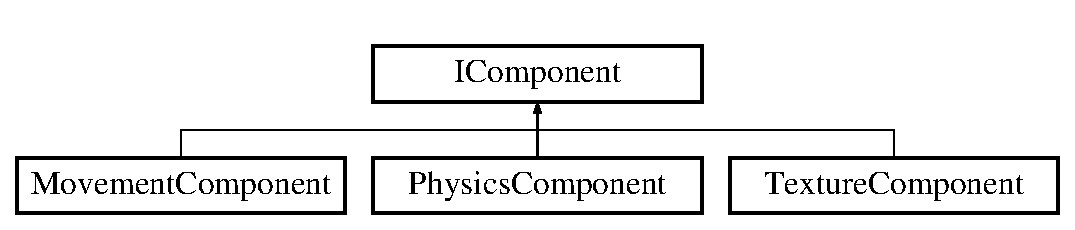
\includegraphics[height=2.000000cm]{class_i_component}
\end{center}
\end{figure}
\subsection*{Public Member Functions}
\begin{DoxyCompactItemize}
\item 
void \mbox{\hyperlink{class_i_component_a4bd5209b8e63446a7fa7d8bf52512590}{Attach\+Game\+Object}} (\mbox{\hyperlink{class_game_object}{Game\+Object}} $\ast$p\+Game\+Object)
\begin{DoxyCompactList}\small\item\em Attaches a game object to the component. \end{DoxyCompactList}\item 
\mbox{\Hypertarget{class_i_component_af1ab9b7331c157bad637ccc9b1f84738}\label{class_i_component_af1ab9b7331c157bad637ccc9b1f84738}} 
void \mbox{\hyperlink{class_i_component_af1ab9b7331c157bad637ccc9b1f84738}{Detach\+Game\+Object}} ()
\begin{DoxyCompactList}\small\item\em Detaches a game object to the component. \end{DoxyCompactList}\item 
\mbox{\Hypertarget{class_i_component_a1ad033cc00f92661575c019a3e5f9e25}\label{class_i_component_a1ad033cc00f92661575c019a3e5f9e25}} 
unsigned int \mbox{\hyperlink{class_i_component_a1ad033cc00f92661575c019a3e5f9e25}{Get\+ID}} ()
\begin{DoxyCompactList}\small\item\em Returns the component ID. \end{DoxyCompactList}\item 
\mbox{\Hypertarget{class_i_component_a7ccd24d547d0a4850071db70afdc49e9}\label{class_i_component_a7ccd24d547d0a4850071db70afdc49e9}} 
void \mbox{\hyperlink{class_i_component_a7ccd24d547d0a4850071db70afdc49e9}{Set\+ID}} (unsigned int new\+ID)
\begin{DoxyCompactList}\small\item\em Sets the component ID. \end{DoxyCompactList}\item 
\mbox{\Hypertarget{class_i_component_ab1a616cdfb3812f3aabdb97666c71116}\label{class_i_component_ab1a616cdfb3812f3aabdb97666c71116}} 
virtual \mbox{\hyperlink{class_i_component_ab1a616cdfb3812f3aabdb97666c71116}{$\sim$\+I\+Component}} ()=default
\begin{DoxyCompactList}\small\item\em Virtual destructor. \end{DoxyCompactList}\end{DoxyCompactItemize}
\subsection*{Protected Attributes}
\begin{DoxyCompactItemize}
\item 
\mbox{\Hypertarget{class_i_component_a2a03e5373f9b633031ed22597ab051ce}\label{class_i_component_a2a03e5373f9b633031ed22597ab051ce}} 
\mbox{\hyperlink{class_game_object}{Game\+Object}} $\ast$ \mbox{\hyperlink{class_i_component_a2a03e5373f9b633031ed22597ab051ce}{m\+\_\+p\+Game\+Object}}
\begin{DoxyCompactList}\small\item\em \mbox{\hyperlink{class_game_object}{Game\+Object}} attached to this component. \end{DoxyCompactList}\end{DoxyCompactItemize}


\subsection{Detailed Description}
Interface for Components. 

\subsection{Member Function Documentation}
\mbox{\Hypertarget{class_i_component_a4bd5209b8e63446a7fa7d8bf52512590}\label{class_i_component_a4bd5209b8e63446a7fa7d8bf52512590}} 
\index{I\+Component@{I\+Component}!Attach\+Game\+Object@{Attach\+Game\+Object}}
\index{Attach\+Game\+Object@{Attach\+Game\+Object}!I\+Component@{I\+Component}}
\subsubsection{\texorpdfstring{Attach\+Game\+Object()}{AttachGameObject()}}
{\footnotesize\ttfamily void I\+Component\+::\+Attach\+Game\+Object (\begin{DoxyParamCaption}\item[{\mbox{\hyperlink{class_game_object}{Game\+Object}} $\ast$}]{p\+Game\+Object }\end{DoxyParamCaption})\hspace{0.3cm}{\ttfamily [inline]}}



Attaches a game object to the component. 


\begin{DoxyParams}{Parameters}
{\em p\+Game\+Object} & Pointer to game object to attach to. \\
\hline
\end{DoxyParams}


The documentation for this class was generated from the following file\+:\begin{DoxyCompactItemize}
\item 
Source/\+Logic/\+Game\+Objects/\mbox{\hyperlink{_i_component_8h}{I\+Component.\+h}}\end{DoxyCompactItemize}

\hypertarget{class_i_event_handler}{}\section{I\+Event\+Handler Class Reference}
\label{class_i_event_handler}\index{I\+Event\+Handler@{I\+Event\+Handler}}


Interface for \mbox{\hyperlink{struct_event}{Event}} handlers.  




{\ttfamily \#include $<$Event\+System.\+h$>$}

Inheritance diagram for I\+Event\+Handler\+:\begin{figure}[H]
\begin{center}
\leavevmode
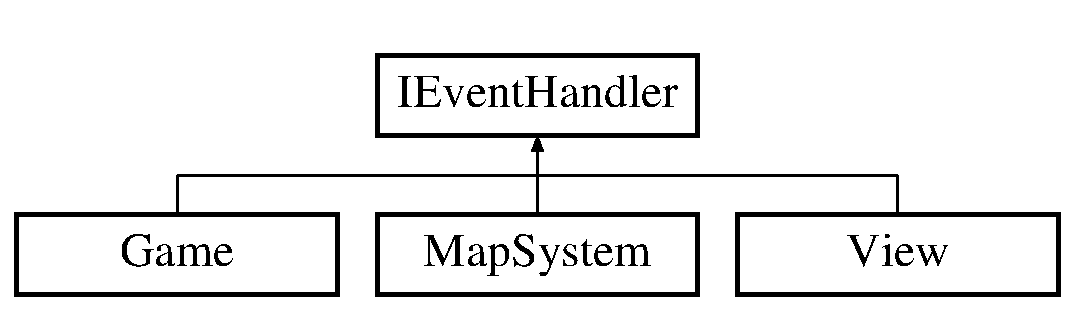
\includegraphics[height=2.000000cm]{class_i_event_handler}
\end{center}
\end{figure}
\subsection*{Public Member Functions}
\begin{DoxyCompactItemize}
\item 
virtual void \mbox{\hyperlink{class_i_event_handler_a2174b40d97b1be9b01bbdf77597dff26}{Handle\+Event}} (\mbox{\hyperlink{struct_event}{Event}} $\ast$p\+Event)=0
\begin{DoxyCompactList}\small\item\em Handles the event. \end{DoxyCompactList}\end{DoxyCompactItemize}


\subsection{Detailed Description}
Interface for \mbox{\hyperlink{struct_event}{Event}} handlers. 

\subsection{Member Function Documentation}
\mbox{\Hypertarget{class_i_event_handler_a2174b40d97b1be9b01bbdf77597dff26}\label{class_i_event_handler_a2174b40d97b1be9b01bbdf77597dff26}} 
\index{I\+Event\+Handler@{I\+Event\+Handler}!Handle\+Event@{Handle\+Event}}
\index{Handle\+Event@{Handle\+Event}!I\+Event\+Handler@{I\+Event\+Handler}}
\subsubsection{\texorpdfstring{Handle\+Event()}{HandleEvent()}}
{\footnotesize\ttfamily virtual void I\+Event\+Handler\+::\+Handle\+Event (\begin{DoxyParamCaption}\item[{\mbox{\hyperlink{struct_event}{Event}} $\ast$}]{p\+Event }\end{DoxyParamCaption})\hspace{0.3cm}{\ttfamily [pure virtual]}}



Handles the event. 


\begin{DoxyParams}{Parameters}
{\em event} & \mbox{\hyperlink{struct_event}{Event}} to handle \\
\hline
\end{DoxyParams}


Implemented in \mbox{\hyperlink{class_map_system_aa9043b7359220c63274a6d0b520bfe10}{Map\+System}}, \mbox{\hyperlink{class_game_a379673c1cde729d801e6f14f7b394810}{Game}}, and \mbox{\hyperlink{class_view_abaeae948fb2fbc2585756afc6962b66e}{View}}.



The documentation for this class was generated from the following file\+:\begin{DoxyCompactItemize}
\item 
Source/\+Logic/\+Events/\mbox{\hyperlink{_event_system_8h}{Event\+System.\+h}}\end{DoxyCompactItemize}

\hypertarget{class_input_interpreter}{}\section{Input\+Interpreter Class Reference}
\label{class_input_interpreter}\index{Input\+Interpreter@{Input\+Interpreter}}


Interpretes user input into commands.  




{\ttfamily \#include $<$Input\+Interpreter.\+h$>$}

\subsection*{Public Member Functions}
\begin{DoxyCompactItemize}
\item 
\mbox{\Hypertarget{class_input_interpreter_a0a763fbc159f1a3841d0c496a7608b74}\label{class_input_interpreter_a0a763fbc159f1a3841d0c496a7608b74}} 
bool \mbox{\hyperlink{class_input_interpreter_a0a763fbc159f1a3841d0c496a7608b74}{Init}} ()
\begin{DoxyCompactList}\small\item\em Initilaizes the interpreter. \end{DoxyCompactList}\item 
\mbox{\Hypertarget{class_input_interpreter_a8d78a3a9a91561a4dbd67f5b301b25cf}\label{class_input_interpreter_a8d78a3a9a91561a4dbd67f5b301b25cf}} 
void \mbox{\hyperlink{class_input_interpreter_a8d78a3a9a91561a4dbd67f5b301b25cf}{Clean\+Up}} ()
\begin{DoxyCompactList}\small\item\em Cleans up the interpreter from memory. \end{DoxyCompactList}\item 
\mbox{\Hypertarget{class_input_interpreter_a9a1a36c64d4bfbe69fb98abcfe731c62}\label{class_input_interpreter_a9a1a36c64d4bfbe69fb98abcfe731c62}} 
\mbox{\hyperlink{class_key_command}{Key\+Command}} \mbox{\hyperlink{class_input_interpreter_a9a1a36c64d4bfbe69fb98abcfe731c62}{Interpret\+Key\+Input}} (S\+D\+L\+\_\+\+Keyboard\+Event \&key\+Event)
\begin{DoxyCompactList}\small\item\em interprets key presses \end{DoxyCompactList}\end{DoxyCompactItemize}


\subsection{Detailed Description}
Interpretes user input into commands. 

The documentation for this class was generated from the following files\+:\begin{DoxyCompactItemize}
\item 
Source/\+Logic/\+Input/\mbox{\hyperlink{_input_interpreter_8h}{Input\+Interpreter.\+h}}\item 
Source/\+Logic/\+Input/Input\+Interpreter.\+cpp\end{DoxyCompactItemize}

\hypertarget{class_input_system}{}\section{Input\+System Class Reference}
\label{class_input_system}\index{Input\+System@{Input\+System}}


Handles sdl input events then, tells \mbox{\hyperlink{class_input_interpreter}{Input\+Interpreter}} to interpret, then sends the interpreted input to \mbox{\hyperlink{class_game}{Game}}.  




{\ttfamily \#include $<$Input\+System.\+h$>$}

\subsection*{Public Member Functions}
\begin{DoxyCompactItemize}
\item 
\mbox{\Hypertarget{class_input_system_a00623e541ff826b6feea56c06dd662ac}\label{class_input_system_a00623e541ff826b6feea56c06dd662ac}} 
void \mbox{\hyperlink{class_input_system_a00623e541ff826b6feea56c06dd662ac}{Handle\+Key\+Input}} (S\+D\+L\+\_\+\+Event \&key\+Event)
\begin{DoxyCompactList}\small\item\em Handles key input. \end{DoxyCompactList}\item 
\mbox{\Hypertarget{class_input_system_a10fd1e6d546a9a6d3d6ea46938c0c458}\label{class_input_system_a10fd1e6d546a9a6d3d6ea46938c0c458}} 
bool \mbox{\hyperlink{class_input_system_a10fd1e6d546a9a6d3d6ea46938c0c458}{Init}} (\mbox{\hyperlink{class_game}{Game}} $\ast$p\+Game)
\begin{DoxyCompactList}\small\item\em Initializes input system. \end{DoxyCompactList}\item 
\mbox{\Hypertarget{class_input_system_aff8fc30adb0eeba8ffb280ca2460b9ac}\label{class_input_system_aff8fc30adb0eeba8ffb280ca2460b9ac}} 
void \mbox{\hyperlink{class_input_system_aff8fc30adb0eeba8ffb280ca2460b9ac}{Clean\+Up}} ()
\begin{DoxyCompactList}\small\item\em Cleans input system from memory. \end{DoxyCompactList}\end{DoxyCompactItemize}


\subsection{Detailed Description}
Handles sdl input events then, tells \mbox{\hyperlink{class_input_interpreter}{Input\+Interpreter}} to interpret, then sends the interpreted input to \mbox{\hyperlink{class_game}{Game}}. 

The documentation for this class was generated from the following files\+:\begin{DoxyCompactItemize}
\item 
Source/\+Logic/\+Input/\mbox{\hyperlink{_input_system_8h}{Input\+System.\+h}}\item 
Source/\+Logic/\+Input/Input\+System.\+cpp\end{DoxyCompactItemize}

\hypertarget{class_i_renderable}{}\section{I\+Renderable Class Reference}
\label{class_i_renderable}\index{I\+Renderable@{I\+Renderable}}


Interface for anything renderable.  




{\ttfamily \#include $<$I\+Renderable.\+h$>$}

Inheritance diagram for I\+Renderable\+:\begin{figure}[H]
\begin{center}
\leavevmode
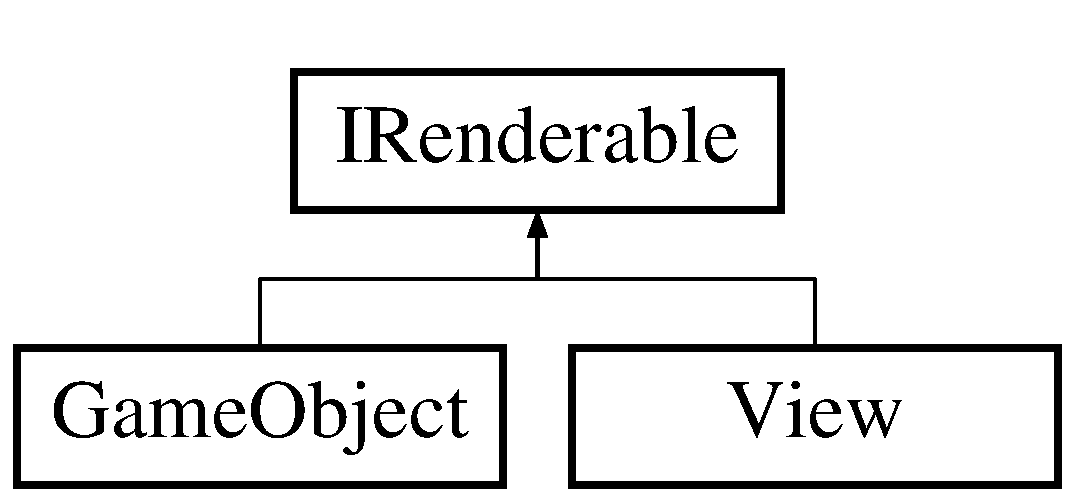
\includegraphics[height=2.000000cm]{class_i_renderable}
\end{center}
\end{figure}
\subsection*{Public Member Functions}
\begin{DoxyCompactItemize}
\item 
\mbox{\Hypertarget{class_i_renderable_af51ff75319f20a9bdefd76abe8060986}\label{class_i_renderable_af51ff75319f20a9bdefd76abe8060986}} 
virtual void \mbox{\hyperlink{class_i_renderable_af51ff75319f20a9bdefd76abe8060986}{Render}} ()=0
\begin{DoxyCompactList}\small\item\em Interface function for a renderable. \end{DoxyCompactList}\end{DoxyCompactItemize}


\subsection{Detailed Description}
Interface for anything renderable. 

The documentation for this class was generated from the following file\+:\begin{DoxyCompactItemize}
\item 
Source/\+Views/\mbox{\hyperlink{_i_renderable_8h}{I\+Renderable.\+h}}\end{DoxyCompactItemize}

\hypertarget{class_i_resource}{}\section{I\+Resource Class Reference}
\label{class_i_resource}\index{I\+Resource@{I\+Resource}}


Interface for all engine resoureces.  




{\ttfamily \#include $<$Resource\+System.\+h$>$}

Inheritance diagram for I\+Resource\+:\begin{figure}[H]
\begin{center}
\leavevmode
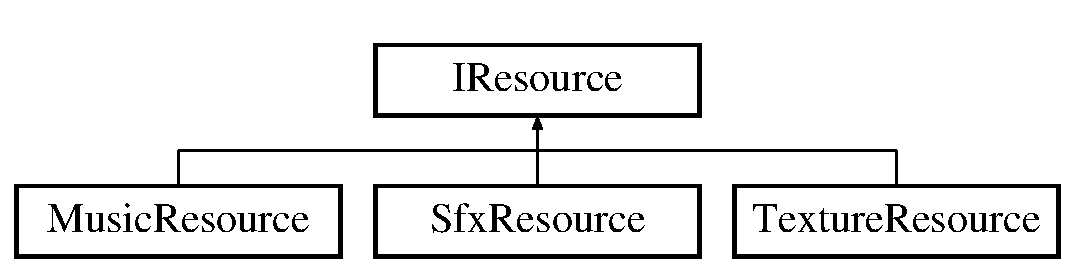
\includegraphics[height=2.000000cm]{class_i_resource}
\end{center}
\end{figure}
\subsection*{Public Types}
\begin{DoxyCompactItemize}
\item 
\mbox{\Hypertarget{class_i_resource_a693b751055bf043ebcd424a89831397f}\label{class_i_resource_a693b751055bf043ebcd424a89831397f}} 
enum \mbox{\hyperlink{class_i_resource_a693b751055bf043ebcd424a89831397f}{Type}} \{ {\bfseries k\+Texture}, 
{\bfseries k\+Sfx}, 
{\bfseries k\+Music}, 
{\bfseries k\+Num\+Of\+Types}
 \}
\begin{DoxyCompactList}\small\item\em Resource types. \end{DoxyCompactList}\end{DoxyCompactItemize}
\subsection*{Public Member Functions}
\begin{DoxyCompactItemize}
\item 
\mbox{\Hypertarget{class_i_resource_a733c11618b98cacd022566dc6fce29c6}\label{class_i_resource_a733c11618b98cacd022566dc6fce29c6}} 
\mbox{\hyperlink{class_i_resource_a693b751055bf043ebcd424a89831397f}{Type}} {\bfseries Get\+Type} ()
\item 
\mbox{\Hypertarget{class_i_resource_a445ec646f31cc4fb46fa94a666d9c891}\label{class_i_resource_a445ec646f31cc4fb46fa94a666d9c891}} 
void {\bfseries Set\+Type} (const \mbox{\hyperlink{class_i_resource_a693b751055bf043ebcd424a89831397f}{Type}} \&type)
\end{DoxyCompactItemize}
\subsection*{Protected Attributes}
\begin{DoxyCompactItemize}
\item 
\mbox{\hyperlink{class_i_resource_a693b751055bf043ebcd424a89831397f}{Type}} \mbox{\hyperlink{class_i_resource_ada72a3487016b965f957c8d89555d84b}{m\+\_\+type}}
\begin{DoxyCompactList}\small\item\em Resource ID. \end{DoxyCompactList}\end{DoxyCompactItemize}


\subsection{Detailed Description}
Interface for all engine resoureces. 

\subsection{Member Data Documentation}
\mbox{\Hypertarget{class_i_resource_ada72a3487016b965f957c8d89555d84b}\label{class_i_resource_ada72a3487016b965f957c8d89555d84b}} 
\index{I\+Resource@{I\+Resource}!m\+\_\+type@{m\+\_\+type}}
\index{m\+\_\+type@{m\+\_\+type}!I\+Resource@{I\+Resource}}
\subsubsection{\texorpdfstring{m\+\_\+type}{m\_type}}
{\footnotesize\ttfamily \mbox{\hyperlink{class_i_resource_a693b751055bf043ebcd424a89831397f}{Type}} I\+Resource\+::m\+\_\+type\hspace{0.3cm}{\ttfamily [protected]}}



Resource ID. 

Resource type 

The documentation for this class was generated from the following file\+:\begin{DoxyCompactItemize}
\item 
Source/\+Views/\mbox{\hyperlink{_resource_system_8h}{Resource\+System.\+h}}\end{DoxyCompactItemize}

\hypertarget{class_i_updatable}{}\section{I\+Updatable Class Reference}
\label{class_i_updatable}\index{I\+Updatable@{I\+Updatable}}


Interface for anything that updates.  




{\ttfamily \#include $<$I\+Updatable.\+h$>$}

Inheritance diagram for I\+Updatable\+:\begin{figure}[H]
\begin{center}
\leavevmode
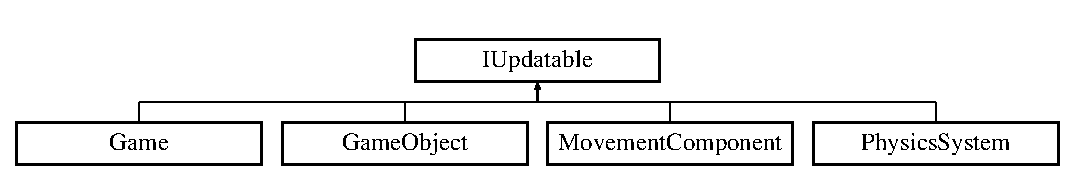
\includegraphics[height=1.985816cm]{class_i_updatable}
\end{center}
\end{figure}
\subsection*{Public Member Functions}
\begin{DoxyCompactItemize}
\item 
virtual void \mbox{\hyperlink{class_i_updatable_a291a40a3422a0b02ef4c10e1d1570eb0}{Update}} (float delta\+Time\+\_\+sec)=0
\begin{DoxyCompactList}\small\item\em Update interface function. \end{DoxyCompactList}\end{DoxyCompactItemize}


\subsection{Detailed Description}
Interface for anything that updates. 

\subsection{Member Function Documentation}
\mbox{\Hypertarget{class_i_updatable_a291a40a3422a0b02ef4c10e1d1570eb0}\label{class_i_updatable_a291a40a3422a0b02ef4c10e1d1570eb0}} 
\index{I\+Updatable@{I\+Updatable}!Update@{Update}}
\index{Update@{Update}!I\+Updatable@{I\+Updatable}}
\subsubsection{\texorpdfstring{Update()}{Update()}}
{\footnotesize\ttfamily virtual void I\+Updatable\+::\+Update (\begin{DoxyParamCaption}\item[{float}]{delta\+Time\+\_\+sec }\end{DoxyParamCaption})\hspace{0.3cm}{\ttfamily [pure virtual]}}



Update interface function. 


\begin{DoxyParams}{Parameters}
{\em delat\+Time\+\_\+sec} & Time difference between frames in seconds \\
\hline
\end{DoxyParams}


Implemented in \mbox{\hyperlink{class_physics_system_aabb107eb3795556bff83099d7f3cb710}{Physics\+System}}, \mbox{\hyperlink{class_game_object_a931541422ec57567e1d46436d97b874c}{Game\+Object}}, \mbox{\hyperlink{class_game_a49cc5bc8eee98577d72cd49dfc3c4af5}{Game}}, and \mbox{\hyperlink{class_movement_component_ae366501e0dbaf79deaab508cf5a0b86e}{Movement\+Component}}.



The documentation for this class was generated from the following file\+:\begin{DoxyCompactItemize}
\item 
Source/\+Logic/\mbox{\hyperlink{_i_updatable_8h}{I\+Updatable.\+h}}\end{DoxyCompactItemize}

\hypertarget{class_key_command}{}\section{Key\+Command Class Reference}
\label{class_key_command}\index{Key\+Command@{Key\+Command}}


Represents a keyboard command.  




{\ttfamily \#include $<$Key\+Command.\+h$>$}

Inheritance diagram for Key\+Command\+:\begin{figure}[H]
\begin{center}
\leavevmode
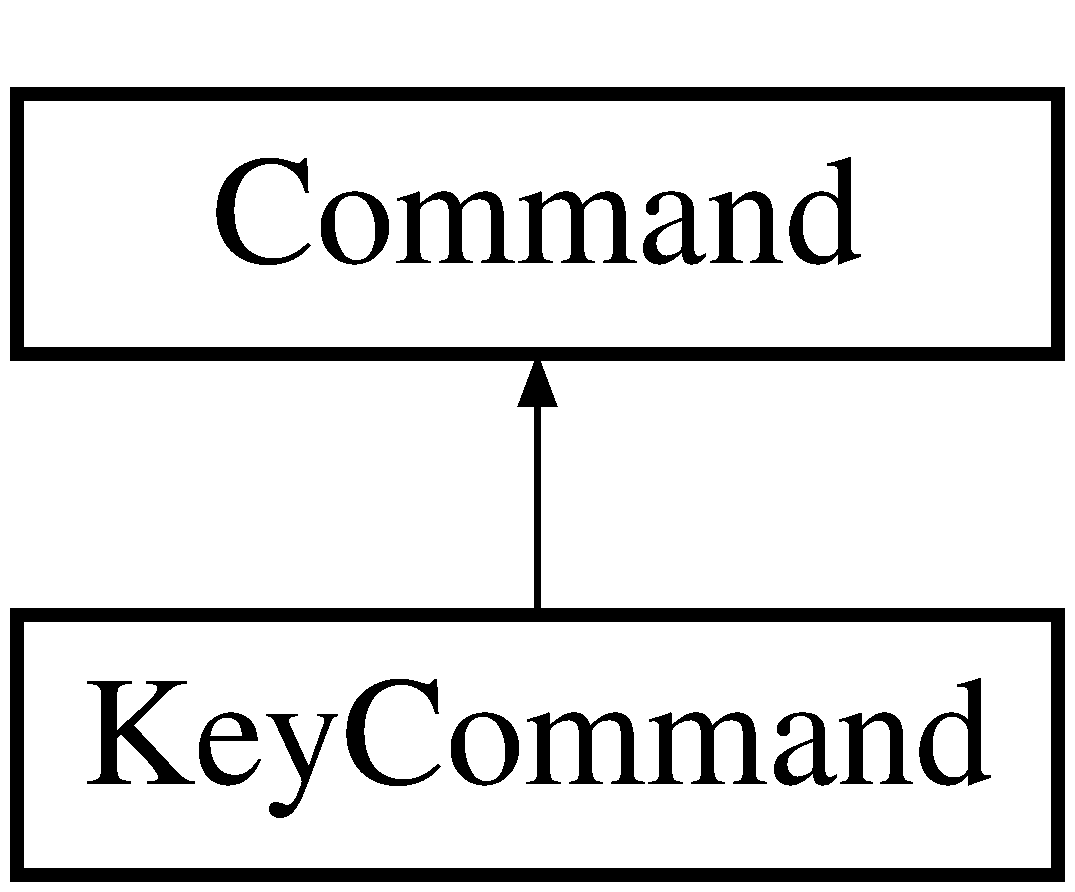
\includegraphics[height=2.000000cm]{class_key_command}
\end{center}
\end{figure}
\subsection*{Public Types}
\begin{DoxyCompactItemize}
\item 
\mbox{\Hypertarget{class_key_command_abd933bd3181a248c86fdd38801647e92}\label{class_key_command_abd933bd3181a248c86fdd38801647e92}} 
enum \mbox{\hyperlink{class_key_command_abd933bd3181a248c86fdd38801647e92}{State}} \{ {\bfseries k\+Invalid}, 
{\bfseries k\+Pressed}, 
{\bfseries k\+Released}, 
{\bfseries k\+Num\+Of\+States}
 \}
\begin{DoxyCompactList}\small\item\em Different key states. \end{DoxyCompactList}\end{DoxyCompactItemize}
\subsection*{Public Member Functions}
\begin{DoxyCompactItemize}
\item 
\mbox{\hyperlink{class_key_command_ad60da4c304d27c3d54aed183e361d9e8}{Key\+Command}} (\mbox{\hyperlink{class_command_a45bbda49e9ee96d262ac651fefffe487}{Command\+::\+Action}} action=Command\+::\+Action\+::k\+Invalid, \mbox{\hyperlink{class_key_command_abd933bd3181a248c86fdd38801647e92}{State}} state=State\+::k\+Invalid, S\+D\+L\+\_\+\+Keycode key=S\+D\+L\+K\+\_\+\+U\+N\+K\+N\+O\+WN)
\item 
\mbox{\Hypertarget{class_key_command_a3de8b2fef57cb8a275c937b9c1424f03}\label{class_key_command_a3de8b2fef57cb8a275c937b9c1424f03}} 
\mbox{\hyperlink{class_key_command_abd933bd3181a248c86fdd38801647e92}{State}} \mbox{\hyperlink{class_key_command_a3de8b2fef57cb8a275c937b9c1424f03}{Get\+State}} ()
\begin{DoxyCompactList}\small\item\em Returns the state. \end{DoxyCompactList}\item 
void \mbox{\hyperlink{class_key_command_a7c899ef655747d0386f55833b3b2b542}{Set\+State}} (\mbox{\hyperlink{class_key_command_abd933bd3181a248c86fdd38801647e92}{State}} state)
\begin{DoxyCompactList}\small\item\em Sets command state. \end{DoxyCompactList}\end{DoxyCompactItemize}
\subsection*{Additional Inherited Members}


\subsection{Detailed Description}
Represents a keyboard command. 

\subsection{Constructor \& Destructor Documentation}
\mbox{\Hypertarget{class_key_command_ad60da4c304d27c3d54aed183e361d9e8}\label{class_key_command_ad60da4c304d27c3d54aed183e361d9e8}} 
\index{Key\+Command@{Key\+Command}!Key\+Command@{Key\+Command}}
\index{Key\+Command@{Key\+Command}!Key\+Command@{Key\+Command}}
\subsubsection{\texorpdfstring{Key\+Command()}{KeyCommand()}}
{\footnotesize\ttfamily Key\+Command\+::\+Key\+Command (\begin{DoxyParamCaption}\item[{\mbox{\hyperlink{class_command_a45bbda49e9ee96d262ac651fefffe487}{Command\+::\+Action}}}]{action = {\ttfamily Command\+:\+:Action\+:\+:kInvalid},  }\item[{\mbox{\hyperlink{class_key_command_abd933bd3181a248c86fdd38801647e92}{State}}}]{state = {\ttfamily State\+:\+:kInvalid},  }\item[{S\+D\+L\+\_\+\+Keycode}]{key = {\ttfamily SDLK\+\_\+UNKNOWN} }\end{DoxyParamCaption})}

Constructor 
\begin{DoxyParams}{Parameters}
{\em action} & \mbox{\hyperlink{class_command}{Command}} action \\
\hline
{\em state} & \mbox{\hyperlink{class_command}{Command}} state \\
\hline
{\em key} & Key this command represents \\
\hline
\end{DoxyParams}


\subsection{Member Function Documentation}
\mbox{\Hypertarget{class_key_command_a7c899ef655747d0386f55833b3b2b542}\label{class_key_command_a7c899ef655747d0386f55833b3b2b542}} 
\index{Key\+Command@{Key\+Command}!Set\+State@{Set\+State}}
\index{Set\+State@{Set\+State}!Key\+Command@{Key\+Command}}
\subsubsection{\texorpdfstring{Set\+State()}{SetState()}}
{\footnotesize\ttfamily void Key\+Command\+::\+Set\+State (\begin{DoxyParamCaption}\item[{\mbox{\hyperlink{class_key_command_abd933bd3181a248c86fdd38801647e92}{State}}}]{state }\end{DoxyParamCaption})\hspace{0.3cm}{\ttfamily [inline]}}



Sets command state. 


\begin{DoxyParams}{Parameters}
{\em state} & State to be set \\
\hline
\end{DoxyParams}


The documentation for this class was generated from the following files\+:\begin{DoxyCompactItemize}
\item 
Source/\+Logic/\+Input/\mbox{\hyperlink{_key_command_8h}{Key\+Command.\+h}}\item 
Source/\+Logic/\+Input/Key\+Command.\+cpp\end{DoxyCompactItemize}

\hypertarget{structtinyxml2_1_1_long_fits_into_size_t_minus_one}{}\section{tinyxml2\+:\+:Long\+Fits\+Into\+Size\+T\+Minus\+One$<$ bool $>$ Struct Template Reference}
\label{structtinyxml2_1_1_long_fits_into_size_t_minus_one}\index{tinyxml2\+::\+Long\+Fits\+Into\+Size\+T\+Minus\+One$<$ bool $>$@{tinyxml2\+::\+Long\+Fits\+Into\+Size\+T\+Minus\+One$<$ bool $>$}}
\subsection*{Static Public Member Functions}
\begin{DoxyCompactItemize}
\item 
\mbox{\Hypertarget{structtinyxml2_1_1_long_fits_into_size_t_minus_one_a3057710104ab733963eb32fda0bc374c}\label{structtinyxml2_1_1_long_fits_into_size_t_minus_one_a3057710104ab733963eb32fda0bc374c}} 
static bool {\bfseries Fits} (unsigned long value)
\end{DoxyCompactItemize}


The documentation for this struct was generated from the following file\+:\begin{DoxyCompactItemize}
\item 
Source/\+Utils/tinyxml2.\+cpp\end{DoxyCompactItemize}

\hypertarget{structtinyxml2_1_1_long_fits_into_size_t_minus_one_3_01false_01_4}{}\section{tinyxml2\+:\+:Long\+Fits\+Into\+Size\+T\+Minus\+One$<$ false $>$ Struct Template Reference}
\label{structtinyxml2_1_1_long_fits_into_size_t_minus_one_3_01false_01_4}\index{tinyxml2\+::\+Long\+Fits\+Into\+Size\+T\+Minus\+One$<$ false $>$@{tinyxml2\+::\+Long\+Fits\+Into\+Size\+T\+Minus\+One$<$ false $>$}}
\subsection*{Static Public Member Functions}
\begin{DoxyCompactItemize}
\item 
\mbox{\Hypertarget{structtinyxml2_1_1_long_fits_into_size_t_minus_one_3_01false_01_4_a29b01087f38a951276df69d358dc0764}\label{structtinyxml2_1_1_long_fits_into_size_t_minus_one_3_01false_01_4_a29b01087f38a951276df69d358dc0764}} 
static bool {\bfseries Fits} (unsigned long)
\end{DoxyCompactItemize}


The documentation for this struct was generated from the following file\+:\begin{DoxyCompactItemize}
\item 
Source/\+Utils/tinyxml2.\+cpp\end{DoxyCompactItemize}

\hypertarget{struct_map_event}{}\section{Map\+Event Struct Reference}
\label{struct_map_event}\index{Map\+Event@{Map\+Event}}


Structure for Map System Events.  




{\ttfamily \#include $<$Event\+System.\+h$>$}

Inheritance diagram for Map\+Event\+:\begin{figure}[H]
\begin{center}
\leavevmode
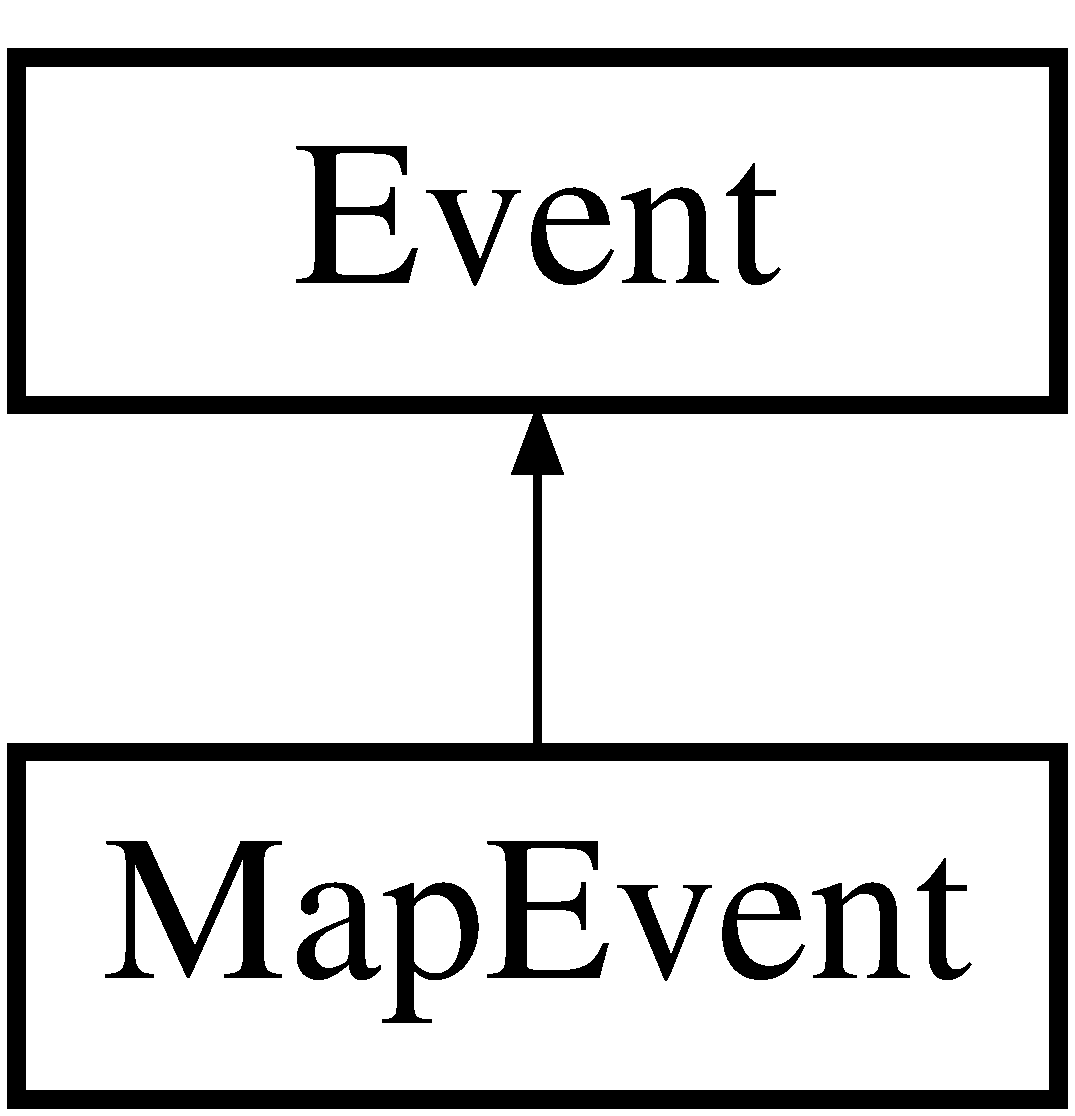
\includegraphics[height=2.000000cm]{struct_map_event}
\end{center}
\end{figure}
\subsection*{Public Attributes}
\begin{DoxyCompactItemize}
\item 
\mbox{\Hypertarget{struct_map_event_a833078363434e917fad009481fd054c0}\label{struct_map_event_a833078363434e917fad009481fd054c0}} 
std\+::vector$<$ \mbox{\hyperlink{class_game_object}{Game\+Object}} $\ast$ $>$ $\ast$ \mbox{\hyperlink{struct_map_event_a833078363434e917fad009481fd054c0}{m\+\_\+p\+Tiles}}
\begin{DoxyCompactList}\small\item\em List of this event\textquotesingle{}s tiles. \end{DoxyCompactList}\end{DoxyCompactItemize}
\subsection*{Additional Inherited Members}


\subsection{Detailed Description}
Structure for Map System Events. 

The documentation for this struct was generated from the following file\+:\begin{DoxyCompactItemize}
\item 
Source/\+Logic/\+Events/\mbox{\hyperlink{_event_system_8h}{Event\+System.\+h}}\end{DoxyCompactItemize}

\hypertarget{class_map_system}{}\section{Map\+System Class Reference}
\label{class_map_system}\index{Map\+System@{Map\+System}}


Handles all tile maps.  




{\ttfamily \#include $<$Map\+System.\+h$>$}

Inheritance diagram for Map\+System\+:\begin{figure}[H]
\begin{center}
\leavevmode
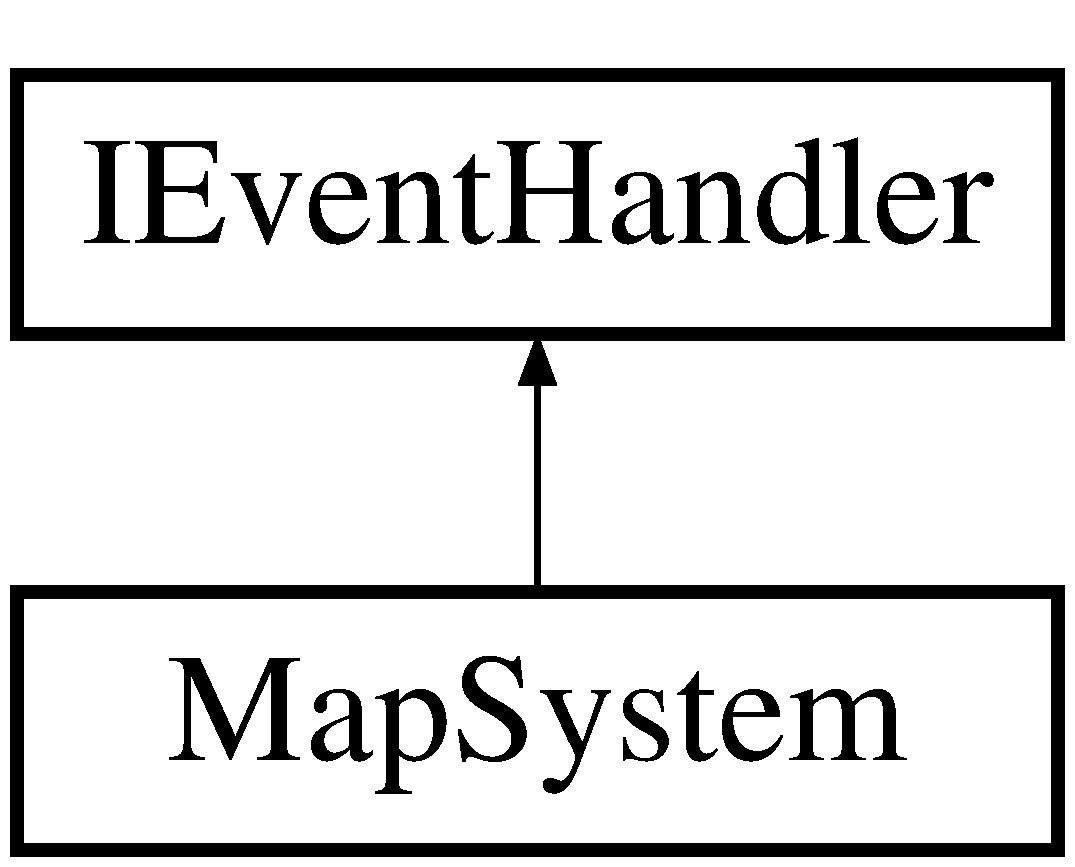
\includegraphics[height=2.000000cm]{class_map_system}
\end{center}
\end{figure}
\subsection*{Public Member Functions}
\begin{DoxyCompactItemize}
\item 
\mbox{\Hypertarget{class_map_system_a4469dda2eb9cda88149e398fba471844}\label{class_map_system_a4469dda2eb9cda88149e398fba471844}} 
bool \mbox{\hyperlink{class_map_system_a4469dda2eb9cda88149e398fba471844}{Load\+Map}} (const char $\ast$file\+Path)
\begin{DoxyCompactList}\small\item\em Loads a map from file. \end{DoxyCompactList}\item 
\mbox{\Hypertarget{class_map_system_a3dd0e0552a3366b66c6c8ddef67572b5}\label{class_map_system_a3dd0e0552a3366b66c6c8ddef67572b5}} 
void \mbox{\hyperlink{class_map_system_a3dd0e0552a3366b66c6c8ddef67572b5}{Clean\+Up}} ()
\begin{DoxyCompactList}\small\item\em Cleans map system. \end{DoxyCompactList}\item 
\mbox{\Hypertarget{class_map_system_aa9043b7359220c63274a6d0b520bfe10}\label{class_map_system_aa9043b7359220c63274a6d0b520bfe10}} 
virtual void \mbox{\hyperlink{class_map_system_aa9043b7359220c63274a6d0b520bfe10}{Handle\+Event}} (\mbox{\hyperlink{struct_event}{Event}} $\ast$p\+Event) override
\begin{DoxyCompactList}\small\item\em Inherited via \mbox{\hyperlink{class_i_event_handler}{I\+Event\+Handler}}. \end{DoxyCompactList}\item 
\mbox{\Hypertarget{class_map_system_a0f01e1a8964dcb9ddd6364e3bccc0d95}\label{class_map_system_a0f01e1a8964dcb9ddd6364e3bccc0d95}} 
void \mbox{\hyperlink{class_map_system_a0f01e1a8964dcb9ddd6364e3bccc0d95}{Set\+Obj\+Pool}} (\mbox{\hyperlink{class_object_pool}{Object\+Pool}} $\ast$p\+Obj\+Pool)
\begin{DoxyCompactList}\small\item\em Sets the game object pool to use. \end{DoxyCompactList}\item 
\mbox{\Hypertarget{class_map_system_a4e9dfbbf00c54d795785eafef680a8de}\label{class_map_system_a4e9dfbbf00c54d795785eafef680a8de}} 
void \mbox{\hyperlink{class_map_system_a4e9dfbbf00c54d795785eafef680a8de}{Set\+Component\+Pool}} (\mbox{\hyperlink{class_component_pool}{Component\+Pool}} $\ast$p\+Comp\+Pool)
\begin{DoxyCompactList}\small\item\em Sets the component pool to use. \end{DoxyCompactList}\end{DoxyCompactItemize}
\subsection*{Static Public Member Functions}
\begin{DoxyCompactItemize}
\item 
\mbox{\Hypertarget{class_map_system_a1c471d051f4d40541f21a7882da835c2}\label{class_map_system_a1c471d051f4d40541f21a7882da835c2}} 
static \mbox{\hyperlink{class_map_system}{Map\+System}} $\ast$ \mbox{\hyperlink{class_map_system_a1c471d051f4d40541f21a7882da835c2}{Get}} ()
\begin{DoxyCompactList}\small\item\em Returns the instance. \end{DoxyCompactList}\item 
\mbox{\Hypertarget{class_map_system_aba3e8e618abf21c5b62a94b8adfa33b9}\label{class_map_system_aba3e8e618abf21c5b62a94b8adfa33b9}} 
static void \mbox{\hyperlink{class_map_system_aba3e8e618abf21c5b62a94b8adfa33b9}{Delete}} ()
\begin{DoxyCompactList}\small\item\em Deletes the instance. \end{DoxyCompactList}\end{DoxyCompactItemize}


\subsection{Detailed Description}
Handles all tile maps. 

The documentation for this class was generated from the following files\+:\begin{DoxyCompactItemize}
\item 
Source/\+Views/\mbox{\hyperlink{_map_system_8h}{Map\+System.\+h}}\item 
Source/\+Views/Map\+System.\+cpp\end{DoxyCompactItemize}

\hypertarget{classtinyxml2_1_1_mem_pool}{}\section{tinyxml2\+:\+:Mem\+Pool Class Reference}
\label{classtinyxml2_1_1_mem_pool}\index{tinyxml2\+::\+Mem\+Pool@{tinyxml2\+::\+Mem\+Pool}}
Inheritance diagram for tinyxml2\+:\+:Mem\+Pool\+:\begin{figure}[H]
\begin{center}
\leavevmode
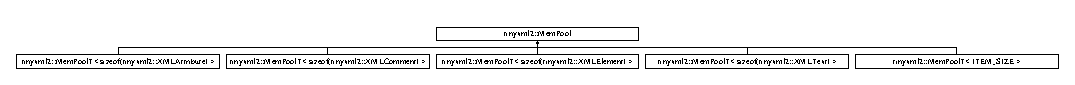
\includegraphics[height=0.691358cm]{classtinyxml2_1_1_mem_pool}
\end{center}
\end{figure}
\subsection*{Public Member Functions}
\begin{DoxyCompactItemize}
\item 
\mbox{\Hypertarget{classtinyxml2_1_1_mem_pool_a0c518d49e3a94bde566f61e13b7240bb}\label{classtinyxml2_1_1_mem_pool_a0c518d49e3a94bde566f61e13b7240bb}} 
virtual int {\bfseries Item\+Size} () const =0
\item 
\mbox{\Hypertarget{classtinyxml2_1_1_mem_pool_a4f977b5fed752c0bbfe5295f469d6449}\label{classtinyxml2_1_1_mem_pool_a4f977b5fed752c0bbfe5295f469d6449}} 
virtual void $\ast$ {\bfseries Alloc} ()=0
\item 
\mbox{\Hypertarget{classtinyxml2_1_1_mem_pool_a49e3bfac2cba2ebd6776b31e571f64f7}\label{classtinyxml2_1_1_mem_pool_a49e3bfac2cba2ebd6776b31e571f64f7}} 
virtual void {\bfseries Free} (void $\ast$)=0
\item 
\mbox{\Hypertarget{classtinyxml2_1_1_mem_pool_ac5804dd1387b2e4de5eef710076a0db1}\label{classtinyxml2_1_1_mem_pool_ac5804dd1387b2e4de5eef710076a0db1}} 
virtual void {\bfseries Set\+Tracked} ()=0
\item 
\mbox{\Hypertarget{classtinyxml2_1_1_mem_pool_a74fcdef9756917c8ae19fbbb4d658ed7}\label{classtinyxml2_1_1_mem_pool_a74fcdef9756917c8ae19fbbb4d658ed7}} 
virtual void {\bfseries Clear} ()=0
\end{DoxyCompactItemize}


The documentation for this class was generated from the following file\+:\begin{DoxyCompactItemize}
\item 
Source/\+Utils/tinyxml2.\+h\end{DoxyCompactItemize}

\hypertarget{classtinyxml2_1_1_mem_pool_t}{}\section{tinyxml2\+:\+:Mem\+PoolT$<$ I\+T\+E\+M\+\_\+\+S\+I\+ZE $>$ Class Template Reference}
\label{classtinyxml2_1_1_mem_pool_t}\index{tinyxml2\+::\+Mem\+Pool\+T$<$ I\+T\+E\+M\+\_\+\+S\+I\+Z\+E $>$@{tinyxml2\+::\+Mem\+Pool\+T$<$ I\+T\+E\+M\+\_\+\+S\+I\+Z\+E $>$}}
Inheritance diagram for tinyxml2\+:\+:Mem\+PoolT$<$ I\+T\+E\+M\+\_\+\+S\+I\+ZE $>$\+:\begin{figure}[H]
\begin{center}
\leavevmode
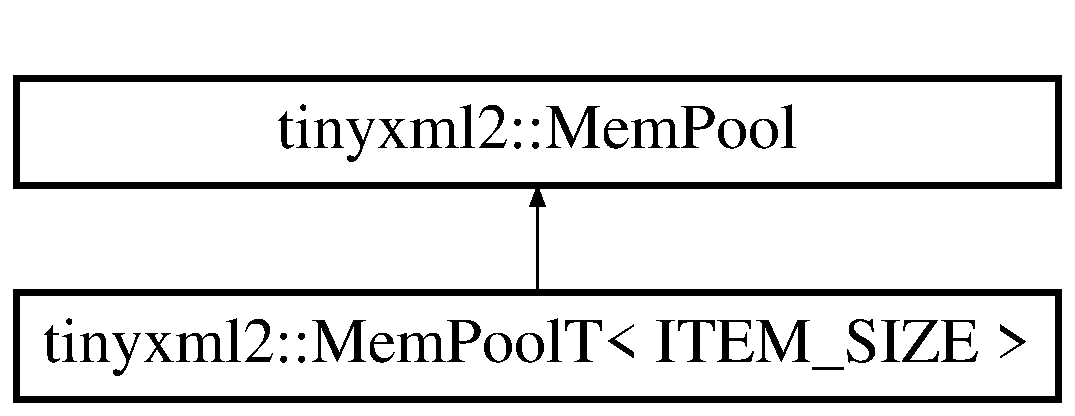
\includegraphics[height=2.000000cm]{classtinyxml2_1_1_mem_pool_t}
\end{center}
\end{figure}
\subsection*{Public Types}
\begin{DoxyCompactItemize}
\item 
\mbox{\Hypertarget{classtinyxml2_1_1_mem_pool_t_a04cf45156e6f913f93972869ff8a1d94}\label{classtinyxml2_1_1_mem_pool_t_a04cf45156e6f913f93972869ff8a1d94}} 
enum \{ {\bfseries I\+T\+E\+M\+S\+\_\+\+P\+E\+R\+\_\+\+B\+L\+O\+CK} = (4 $\ast$ 1024) / I\+T\+E\+M\+\_\+\+S\+I\+ZE
 \}
\end{DoxyCompactItemize}
\subsection*{Public Member Functions}
\begin{DoxyCompactItemize}
\item 
\mbox{\Hypertarget{classtinyxml2_1_1_mem_pool_t_a22d595caa0e9d23aa080f49ca6475fdd}\label{classtinyxml2_1_1_mem_pool_t_a22d595caa0e9d23aa080f49ca6475fdd}} 
void {\bfseries Clear} ()
\item 
\mbox{\Hypertarget{classtinyxml2_1_1_mem_pool_t_a54e4d9b343459ef1731314a99877ff35}\label{classtinyxml2_1_1_mem_pool_t_a54e4d9b343459ef1731314a99877ff35}} 
virtual int {\bfseries Item\+Size} () const
\item 
\mbox{\Hypertarget{classtinyxml2_1_1_mem_pool_t_a445a6c80151ba6268b24ec62a7c84d74}\label{classtinyxml2_1_1_mem_pool_t_a445a6c80151ba6268b24ec62a7c84d74}} 
int {\bfseries Current\+Allocs} () const
\item 
\mbox{\Hypertarget{classtinyxml2_1_1_mem_pool_t_a810fd2b0caf56b8b688e55f2768f96c7}\label{classtinyxml2_1_1_mem_pool_t_a810fd2b0caf56b8b688e55f2768f96c7}} 
virtual void $\ast$ {\bfseries Alloc} ()
\item 
\mbox{\Hypertarget{classtinyxml2_1_1_mem_pool_t_a408ce0918e9d3d5e5e1cc4896944875f}\label{classtinyxml2_1_1_mem_pool_t_a408ce0918e9d3d5e5e1cc4896944875f}} 
virtual void {\bfseries Free} (void $\ast$mem)
\item 
\mbox{\Hypertarget{classtinyxml2_1_1_mem_pool_t_a47eefbd934ef70d973ea41d41ab5f239}\label{classtinyxml2_1_1_mem_pool_t_a47eefbd934ef70d973ea41d41ab5f239}} 
void {\bfseries Trace} (const char $\ast$name)
\item 
\mbox{\Hypertarget{classtinyxml2_1_1_mem_pool_t_aee3c611215ae08cce41a940bf2763027}\label{classtinyxml2_1_1_mem_pool_t_aee3c611215ae08cce41a940bf2763027}} 
void {\bfseries Set\+Tracked} ()
\item 
\mbox{\Hypertarget{classtinyxml2_1_1_mem_pool_t_a3bcdc302ae15d2810e11192321a8f5f1}\label{classtinyxml2_1_1_mem_pool_t_a3bcdc302ae15d2810e11192321a8f5f1}} 
int {\bfseries Untracked} () const
\end{DoxyCompactItemize}


The documentation for this class was generated from the following file\+:\begin{DoxyCompactItemize}
\item 
Source/\+Utils/tinyxml2.\+h\end{DoxyCompactItemize}

\hypertarget{class_movement_component}{}\section{Movement\+Component Class Reference}
\label{class_movement_component}\index{Movement\+Component@{Movement\+Component}}


Component to hold and handle movement data.  




{\ttfamily \#include $<$Movement\+Component.\+h$>$}

Inheritance diagram for Movement\+Component\+:\begin{figure}[H]
\begin{center}
\leavevmode
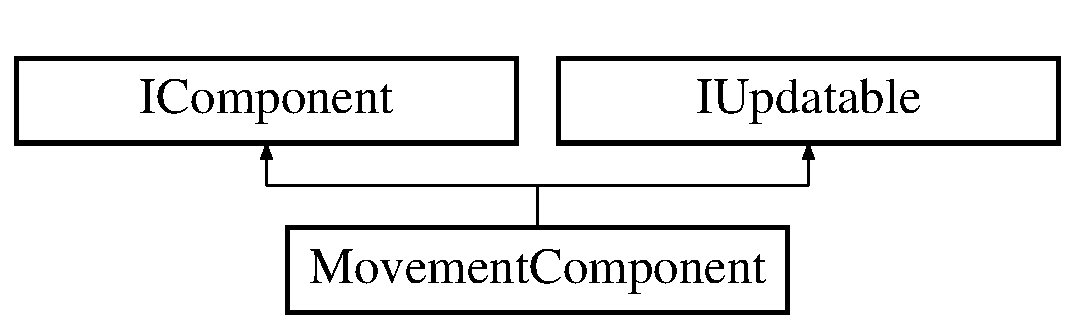
\includegraphics[height=2.000000cm]{class_movement_component}
\end{center}
\end{figure}
\subsection*{Public Member Functions}
\begin{DoxyCompactItemize}
\item 
\mbox{\Hypertarget{class_movement_component_ae366501e0dbaf79deaab508cf5a0b86e}\label{class_movement_component_ae366501e0dbaf79deaab508cf5a0b86e}} 
virtual void \mbox{\hyperlink{class_movement_component_ae366501e0dbaf79deaab508cf5a0b86e}{Update}} (float delta\+Time\+\_\+sec) override
\begin{DoxyCompactList}\small\item\em updates the movement component. \end{DoxyCompactList}\end{DoxyCompactItemize}
\subsection*{Additional Inherited Members}


\subsection{Detailed Description}
Component to hold and handle movement data. 

The documentation for this class was generated from the following files\+:\begin{DoxyCompactItemize}
\item 
Source/\+Logic/\+Game\+Objects/\mbox{\hyperlink{_movement_component_8h}{Movement\+Component.\+h}}\item 
Source/\+Logic/\+Game\+Objects/Movement\+Component.\+cpp\end{DoxyCompactItemize}

\hypertarget{struct_music_event}{}\section{Music\+Event Struct Reference}
\label{struct_music_event}\index{Music\+Event@{Music\+Event}}


Structure for Music Events.  




{\ttfamily \#include $<$Event\+System.\+h$>$}

Inheritance diagram for Music\+Event\+:\begin{figure}[H]
\begin{center}
\leavevmode
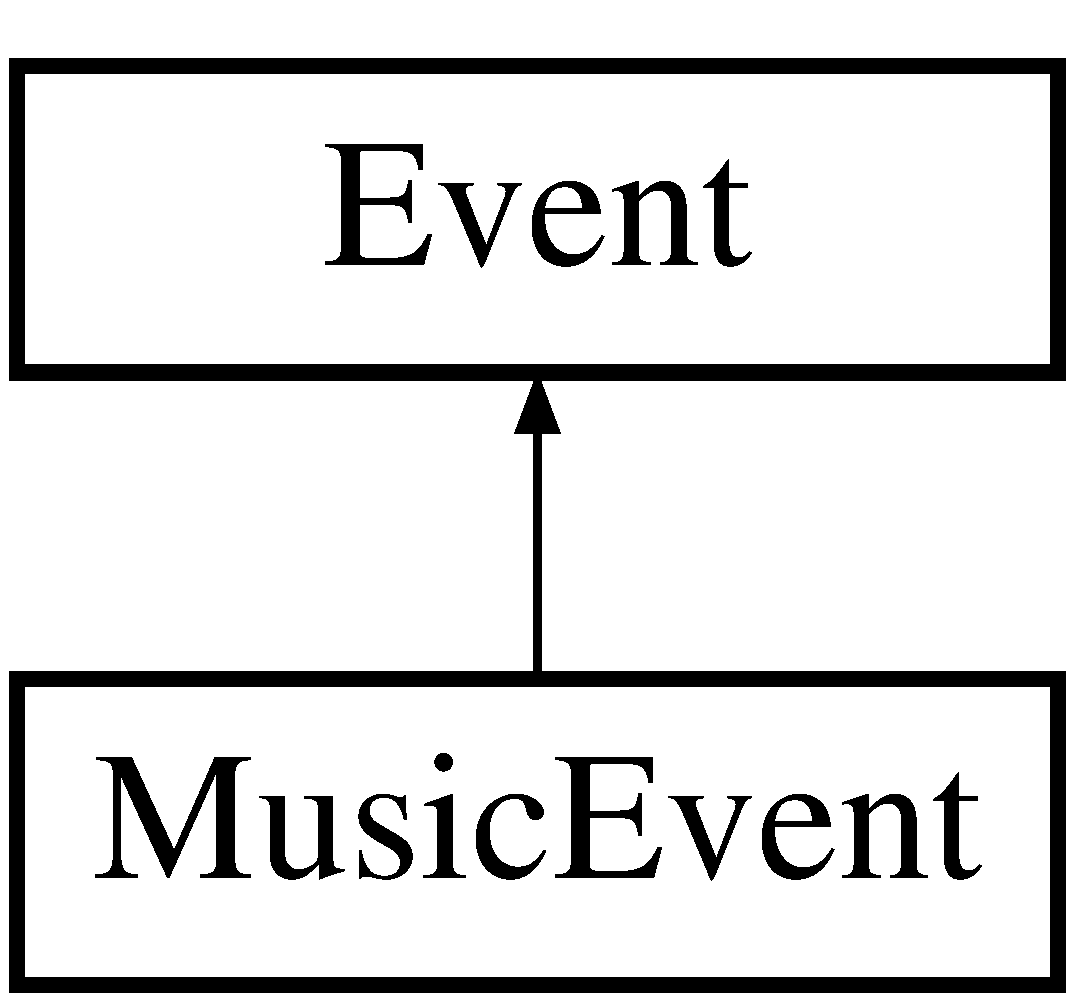
\includegraphics[height=2.000000cm]{struct_music_event}
\end{center}
\end{figure}
\subsection*{Public Attributes}
\begin{DoxyCompactItemize}
\item 
\mbox{\Hypertarget{struct_music_event_a3e703e2628fef9339308ffeee1afdb77}\label{struct_music_event_a3e703e2628fef9339308ffeee1afdb77}} 
std\+::string \mbox{\hyperlink{struct_music_event_a3e703e2628fef9339308ffeee1afdb77}{m\+\_\+music\+Name}}
\begin{DoxyCompactList}\small\item\em Name of the music. \end{DoxyCompactList}\item 
\mbox{\Hypertarget{struct_music_event_a64b7bbf0eeb292bf122ec18ba8e72916}\label{struct_music_event_a64b7bbf0eeb292bf122ec18ba8e72916}} 
std\+::string \mbox{\hyperlink{struct_music_event_a64b7bbf0eeb292bf122ec18ba8e72916}{m\+\_\+music\+File}}
\begin{DoxyCompactList}\small\item\em Filename for the music. \end{DoxyCompactList}\end{DoxyCompactItemize}
\subsection*{Additional Inherited Members}


\subsection{Detailed Description}
Structure for Music Events. 

The documentation for this struct was generated from the following file\+:\begin{DoxyCompactItemize}
\item 
Source/\+Logic/\+Events/\mbox{\hyperlink{_event_system_8h}{Event\+System.\+h}}\end{DoxyCompactItemize}

\hypertarget{struct_music_resource}{}\section{Music\+Resource Struct Reference}
\label{struct_music_resource}\index{Music\+Resource@{Music\+Resource}}


Represents a Music resource.  




{\ttfamily \#include $<$Resource\+System.\+h$>$}

Inheritance diagram for Music\+Resource\+:\begin{figure}[H]
\begin{center}
\leavevmode
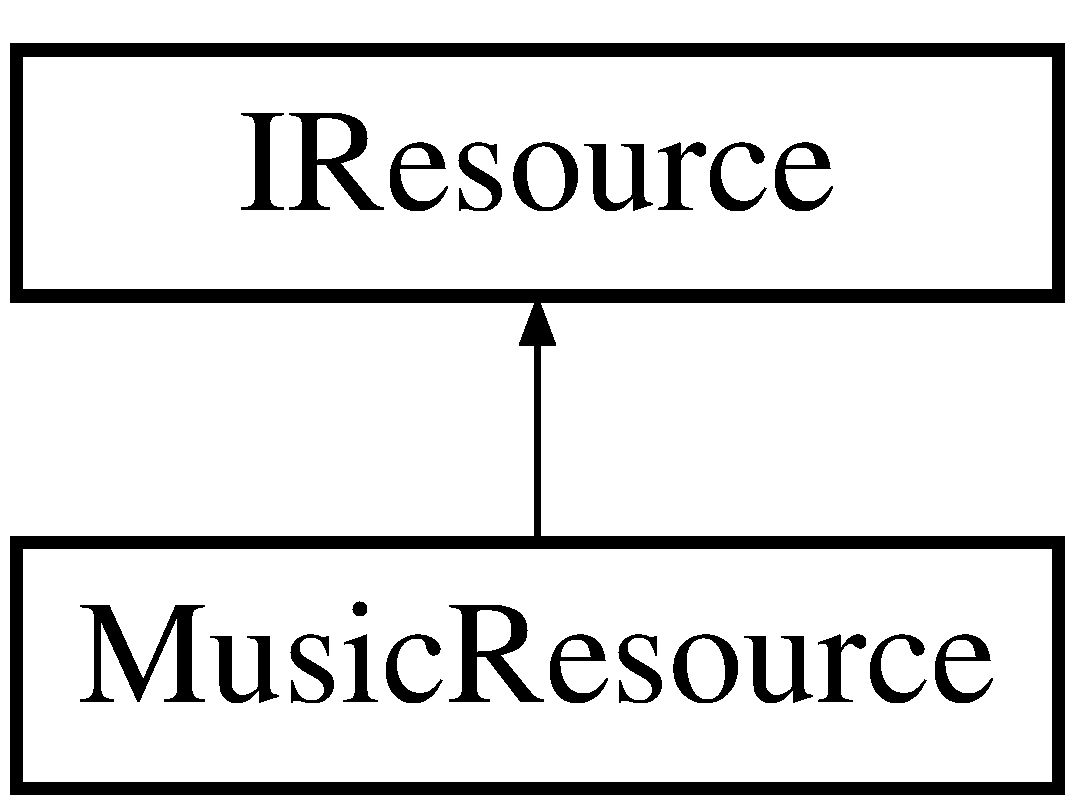
\includegraphics[height=2.000000cm]{struct_music_resource}
\end{center}
\end{figure}
\subsection*{Public Attributes}
\begin{DoxyCompactItemize}
\item 
\mbox{\Hypertarget{struct_music_resource_a8facd21a3775e85e15e4d0c7c5046e4b}\label{struct_music_resource_a8facd21a3775e85e15e4d0c7c5046e4b}} 
Mix\+\_\+\+Music $\ast$ \mbox{\hyperlink{struct_music_resource_a8facd21a3775e85e15e4d0c7c5046e4b}{m\+\_\+p\+Music}}
\begin{DoxyCompactList}\small\item\em Music this resource represents. \end{DoxyCompactList}\end{DoxyCompactItemize}
\subsection*{Additional Inherited Members}


\subsection{Detailed Description}
Represents a Music resource. 

The documentation for this struct was generated from the following file\+:\begin{DoxyCompactItemize}
\item 
Source/\+Views/\mbox{\hyperlink{_resource_system_8h}{Resource\+System.\+h}}\end{DoxyCompactItemize}

\hypertarget{class_object_pool}{}\section{Object\+Pool Class Reference}
\label{class_object_pool}\index{Object\+Pool@{Object\+Pool}}


Pool of Game\+Objects.  




{\ttfamily \#include $<$Object\+Pool.\+h$>$}

\subsection*{Public Member Functions}
\begin{DoxyCompactItemize}
\item 
Game\+Object\+Ptr \mbox{\hyperlink{class_object_pool_acbae5f0774df14a2ddccc0786c3863c3}{Create\+Game\+Object}} (const std\+::string \&obj\+Name)
\begin{DoxyCompactList}\small\item\em Creates a game object and returns a Game\+Object\+Ptr to it. \end{DoxyCompactList}\item 
Game\+Object\+Ptr \mbox{\hyperlink{class_object_pool_a49990f34429a9468b2b2344765ac75dd}{Create\+Deep\+Clone\+Game\+Object}} (\mbox{\hyperlink{class_game_object}{Game\+Object}} $\ast$p\+Object\+Prototype)
\begin{DoxyCompactList}\small\item\em Creates game object by performing a deep copy of an object and returns a Game\+Object\+Ptr to it. \end{DoxyCompactList}\item 
void \mbox{\hyperlink{class_object_pool_a074b2f5730a286179cf5e0f5bd9374ce}{Delete\+Game\+Object}} (const unsigned int obj\+ID)
\begin{DoxyCompactList}\small\item\em Frees a game object from the pool. \end{DoxyCompactList}\item 
\mbox{\Hypertarget{class_object_pool_aa8764710e7d98d249aac86b69b0f1263}\label{class_object_pool_aa8764710e7d98d249aac86b69b0f1263}} 
bool \mbox{\hyperlink{class_object_pool_aa8764710e7d98d249aac86b69b0f1263}{Init}} ()
\begin{DoxyCompactList}\small\item\em Initializes the object pool. Returns false if not successful. \end{DoxyCompactList}\item 
\mbox{\Hypertarget{class_object_pool_a1469f91b4960d14f34ab411509ce15cc}\label{class_object_pool_a1469f91b4960d14f34ab411509ce15cc}} 
int \mbox{\hyperlink{class_object_pool_a1469f91b4960d14f34ab411509ce15cc}{Get\+Obj\+Limit}} ()
\begin{DoxyCompactList}\small\item\em Returns game object limit. \end{DoxyCompactList}\end{DoxyCompactItemize}


\subsection{Detailed Description}
Pool of Game\+Objects. 

\subsection{Member Function Documentation}
\mbox{\Hypertarget{class_object_pool_a49990f34429a9468b2b2344765ac75dd}\label{class_object_pool_a49990f34429a9468b2b2344765ac75dd}} 
\index{Object\+Pool@{Object\+Pool}!Create\+Deep\+Clone\+Game\+Object@{Create\+Deep\+Clone\+Game\+Object}}
\index{Create\+Deep\+Clone\+Game\+Object@{Create\+Deep\+Clone\+Game\+Object}!Object\+Pool@{Object\+Pool}}
\subsubsection{\texorpdfstring{Create\+Deep\+Clone\+Game\+Object()}{CreateDeepCloneGameObject()}}
{\footnotesize\ttfamily Game\+Object\+Ptr Object\+Pool\+::\+Create\+Deep\+Clone\+Game\+Object (\begin{DoxyParamCaption}\item[{\mbox{\hyperlink{class_game_object}{Game\+Object}} $\ast$}]{p\+Object\+Prototype }\end{DoxyParamCaption})}



Creates game object by performing a deep copy of an object and returns a Game\+Object\+Ptr to it. 


\begin{DoxyParams}{Parameters}
{\em p\+Object\+Prototype} & The game object to copy. \\
\hline
\end{DoxyParams}
\mbox{\Hypertarget{class_object_pool_acbae5f0774df14a2ddccc0786c3863c3}\label{class_object_pool_acbae5f0774df14a2ddccc0786c3863c3}} 
\index{Object\+Pool@{Object\+Pool}!Create\+Game\+Object@{Create\+Game\+Object}}
\index{Create\+Game\+Object@{Create\+Game\+Object}!Object\+Pool@{Object\+Pool}}
\subsubsection{\texorpdfstring{Create\+Game\+Object()}{CreateGameObject()}}
{\footnotesize\ttfamily Game\+Object\+Ptr Object\+Pool\+::\+Create\+Game\+Object (\begin{DoxyParamCaption}\item[{const std\+::string \&}]{obj\+Name }\end{DoxyParamCaption})}



Creates a game object and returns a Game\+Object\+Ptr to it. 


\begin{DoxyParams}{Parameters}
{\em obj\+Name} & The name of the new \mbox{\hyperlink{class_game_object}{Game\+Object}} \\
\hline
\end{DoxyParams}
\mbox{\Hypertarget{class_object_pool_a074b2f5730a286179cf5e0f5bd9374ce}\label{class_object_pool_a074b2f5730a286179cf5e0f5bd9374ce}} 
\index{Object\+Pool@{Object\+Pool}!Delete\+Game\+Object@{Delete\+Game\+Object}}
\index{Delete\+Game\+Object@{Delete\+Game\+Object}!Object\+Pool@{Object\+Pool}}
\subsubsection{\texorpdfstring{Delete\+Game\+Object()}{DeleteGameObject()}}
{\footnotesize\ttfamily void Object\+Pool\+::\+Delete\+Game\+Object (\begin{DoxyParamCaption}\item[{const unsigned int}]{obj\+ID }\end{DoxyParamCaption})}



Frees a game object from the pool. 


\begin{DoxyParams}{Parameters}
{\em obj\+ID} & ID of the game object to free. \\
\hline
\end{DoxyParams}


The documentation for this class was generated from the following files\+:\begin{DoxyCompactItemize}
\item 
Source/\+Logic/\+Game\+Objects/Object\+Pool.\+h\item 
Source/\+Logic/\+Game\+Objects/Object\+Pool.\+cpp\end{DoxyCompactItemize}

\hypertarget{class_phaze_logger}{}\section{Phaze\+Logger Class Reference}
\label{class_phaze_logger}\index{Phaze\+Logger@{Phaze\+Logger}}


Static class used to handle logging through engine and game.  




{\ttfamily \#include $<$Phaze\+Logger.\+h$>$}

\subsection*{Public Types}
\begin{DoxyCompactItemize}
\item 
enum \mbox{\hyperlink{class_phaze_logger_aa4b09b6a0ed29d067f86782aa369f6b0}{Log\+Category}} \{ \mbox{\hyperlink{class_phaze_logger_aa4b09b6a0ed29d067f86782aa369f6b0a176a473e63c17ccdac91640c67f149bf}{Log\+Category\+::k\+Info}}, 
\mbox{\hyperlink{class_phaze_logger_aa4b09b6a0ed29d067f86782aa369f6b0aec0da41f4e48b52c362303eb27ed5dee}{Log\+Category\+::k\+Warning}}, 
\mbox{\hyperlink{class_phaze_logger_aa4b09b6a0ed29d067f86782aa369f6b0a5a20548c220f372fc701cae6de94040b}{Log\+Category\+::k\+Critical}}, 
{\bfseries k\+Num\+Of\+Categories}
 \}
\begin{DoxyCompactList}\small\item\em Log categories. \end{DoxyCompactList}\end{DoxyCompactItemize}
\subsection*{Public Member Functions}
\begin{DoxyCompactItemize}
\item 
\mbox{\hyperlink{class_phaze_logger_ab57f5e5578fdba0eb6bddc4fae30b681}{Phaze\+Logger}} ()=delete
\end{DoxyCompactItemize}
\subsection*{Static Public Member Functions}
\begin{DoxyCompactItemize}
\item 
\mbox{\Hypertarget{class_phaze_logger_aa6a0a46e3e5a56c449e2c657697d67e7}\label{class_phaze_logger_aa6a0a46e3e5a56c449e2c657697d67e7}} 
static void \mbox{\hyperlink{class_phaze_logger_aa6a0a46e3e5a56c449e2c657697d67e7}{Write\+To\+Log}} (const \mbox{\hyperlink{class_phaze_logger_aa4b09b6a0ed29d067f86782aa369f6b0}{Log\+Category}} category, const std\+::string \&source\+File\+Name, const std\+::string \&dest\+File\+Name, unsigned int line\+Number, const char $\ast$p\+Msg,...)
\begin{DoxyCompactList}\small\item\em Writes to logger. \end{DoxyCompactList}\end{DoxyCompactItemize}


\subsection{Detailed Description}
Static class used to handle logging through engine and game. 

\subsection{Member Enumeration Documentation}
\mbox{\Hypertarget{class_phaze_logger_aa4b09b6a0ed29d067f86782aa369f6b0}\label{class_phaze_logger_aa4b09b6a0ed29d067f86782aa369f6b0}} 
\index{Phaze\+Logger@{Phaze\+Logger}!Log\+Category@{Log\+Category}}
\index{Log\+Category@{Log\+Category}!Phaze\+Logger@{Phaze\+Logger}}
\subsubsection{\texorpdfstring{Log\+Category}{LogCategory}}
{\footnotesize\ttfamily enum \mbox{\hyperlink{class_phaze_logger_aa4b09b6a0ed29d067f86782aa369f6b0}{Phaze\+Logger\+::\+Log\+Category}}\hspace{0.3cm}{\ttfamily [strong]}}



Log categories. 

\begin{DoxyEnumFields}{Enumerator}
\raisebox{\heightof{T}}[0pt][0pt]{\index{k\+Info@{k\+Info}!Phaze\+Logger@{Phaze\+Logger}}\index{Phaze\+Logger@{Phaze\+Logger}!k\+Info@{k\+Info}}}\mbox{\Hypertarget{class_phaze_logger_aa4b09b6a0ed29d067f86782aa369f6b0a176a473e63c17ccdac91640c67f149bf}\label{class_phaze_logger_aa4b09b6a0ed29d067f86782aa369f6b0a176a473e63c17ccdac91640c67f149bf}} 
k\+Info&Logged to file. \\
\hline

\raisebox{\heightof{T}}[0pt][0pt]{\index{k\+Warning@{k\+Warning}!Phaze\+Logger@{Phaze\+Logger}}\index{Phaze\+Logger@{Phaze\+Logger}!k\+Warning@{k\+Warning}}}\mbox{\Hypertarget{class_phaze_logger_aa4b09b6a0ed29d067f86782aa369f6b0aec0da41f4e48b52c362303eb27ed5dee}\label{class_phaze_logger_aa4b09b6a0ed29d067f86782aa369f6b0aec0da41f4e48b52c362303eb27ed5dee}} 
k\+Warning&Logged to file, logged to console in yellow. \\
\hline

\raisebox{\heightof{T}}[0pt][0pt]{\index{k\+Critical@{k\+Critical}!Phaze\+Logger@{Phaze\+Logger}}\index{Phaze\+Logger@{Phaze\+Logger}!k\+Critical@{k\+Critical}}}\mbox{\Hypertarget{class_phaze_logger_aa4b09b6a0ed29d067f86782aa369f6b0a5a20548c220f372fc701cae6de94040b}\label{class_phaze_logger_aa4b09b6a0ed29d067f86782aa369f6b0a5a20548c220f372fc701cae6de94040b}} 
k\+Critical&Logged to file, logged to console in red, will crash if set. \\
\hline

\end{DoxyEnumFields}


\subsection{Constructor \& Destructor Documentation}
\mbox{\Hypertarget{class_phaze_logger_ab57f5e5578fdba0eb6bddc4fae30b681}\label{class_phaze_logger_ab57f5e5578fdba0eb6bddc4fae30b681}} 
\index{Phaze\+Logger@{Phaze\+Logger}!Phaze\+Logger@{Phaze\+Logger}}
\index{Phaze\+Logger@{Phaze\+Logger}!Phaze\+Logger@{Phaze\+Logger}}
\subsubsection{\texorpdfstring{Phaze\+Logger()}{PhazeLogger()}}
{\footnotesize\ttfamily Phaze\+Logger\+::\+Phaze\+Logger (\begin{DoxyParamCaption}{ }\end{DoxyParamCaption})\hspace{0.3cm}{\ttfamily [delete]}}

Constructor Not ment to be invoked 

The documentation for this class was generated from the following files\+:\begin{DoxyCompactItemize}
\item 
Source/\+Utils/\mbox{\hyperlink{_phaze_logger_8h}{Phaze\+Logger.\+h}}\item 
Source/\+Utils/Phaze\+Logger.\+cpp\end{DoxyCompactItemize}

\hypertarget{struct_physics_component}{}\section{Physics\+Component Class Reference}
\label{struct_physics_component}\index{Physics\+Component@{Physics\+Component}}


Component that enables physics.  




{\ttfamily \#include $<$Physics\+Component.\+h$>$}

Inheritance diagram for Physics\+Component\+:\begin{figure}[H]
\begin{center}
\leavevmode
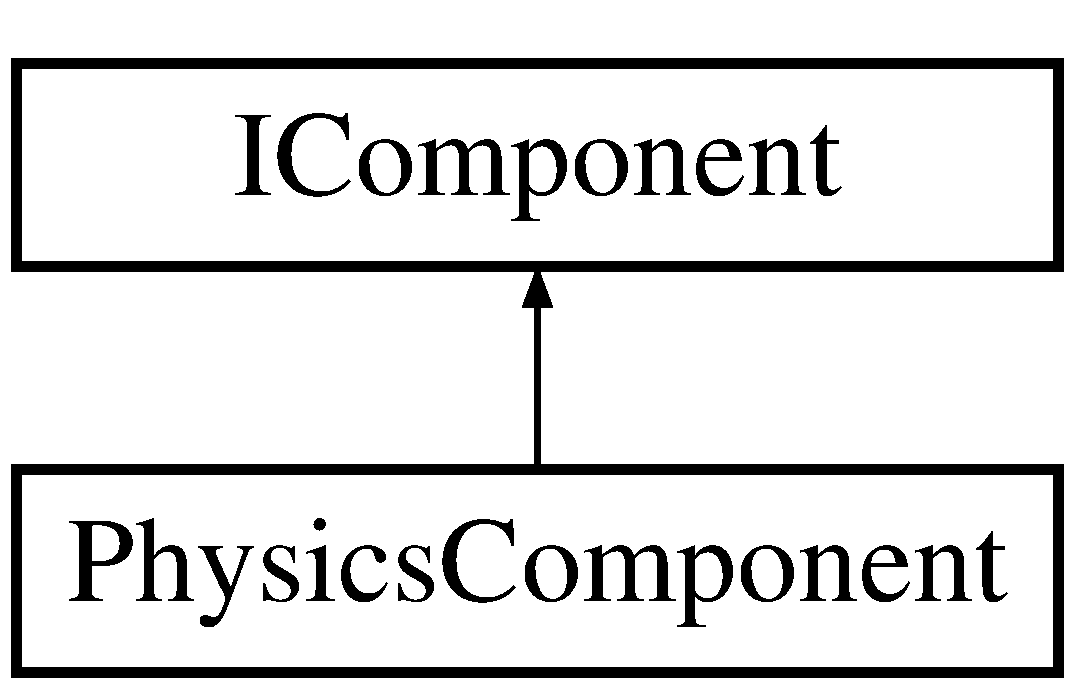
\includegraphics[height=2.000000cm]{struct_physics_component}
\end{center}
\end{figure}
\subsection*{Public Member Functions}
\begin{DoxyCompactItemize}
\item 
\mbox{\Hypertarget{struct_physics_component_a9bf7b6448791c90e0f6f9dc3f3c01536}\label{struct_physics_component_a9bf7b6448791c90e0f6f9dc3f3c01536}} 
void {\bfseries Create\+Body} (const \mbox{\hyperlink{class_physics_system_aa9b3a5f5c38063cdc3a78717250a239e}{Physics\+System\+::\+Rigid\+Body\+Type}} \&type, float x, float y)
\item 
\mbox{\Hypertarget{struct_physics_component_a201127e5510341424e8cdd1663b26d79}\label{struct_physics_component_a201127e5510341424e8cdd1663b26d79}} 
void \mbox{\hyperlink{struct_physics_component_a201127e5510341424e8cdd1663b26d79}{Create\+Fixture}} (const \mbox{\hyperlink{class_physics_system_ac3b7ef40b19864e4ecdec88af3420a89}{Physics\+System\+::\+Polygon\+Shape\+Type}} \&type, float width, float height)
\begin{DoxyCompactList}\small\item\em Creates a fixture for the attached body. \end{DoxyCompactList}\end{DoxyCompactItemize}
\subsection*{Public Attributes}
\begin{DoxyCompactItemize}
\item 
\mbox{\Hypertarget{struct_physics_component_acacb5877966eaecea40298e10e85cfbe}\label{struct_physics_component_acacb5877966eaecea40298e10e85cfbe}} 
b2\+Body $\ast$ \mbox{\hyperlink{struct_physics_component_acacb5877966eaecea40298e10e85cfbe}{m\+\_\+p\+Body}}
\begin{DoxyCompactList}\small\item\em Body of the game object. \end{DoxyCompactList}\item 
\mbox{\Hypertarget{struct_physics_component_a1f890d5f3718a03a8d6ef4a94aa14d41}\label{struct_physics_component_a1f890d5f3718a03a8d6ef4a94aa14d41}} 
b2\+Fixture\+Def \mbox{\hyperlink{struct_physics_component_a1f890d5f3718a03a8d6ef4a94aa14d41}{m\+\_\+fixture\+Def}}
\begin{DoxyCompactList}\small\item\em Fixture Definition. \end{DoxyCompactList}\item 
\mbox{\Hypertarget{struct_physics_component_ae909b17a29234ccba3d4f55e61e7a228}\label{struct_physics_component_ae909b17a29234ccba3d4f55e61e7a228}} 
b2\+Body\+Def \mbox{\hyperlink{struct_physics_component_ae909b17a29234ccba3d4f55e61e7a228}{m\+\_\+body\+Def}}
\begin{DoxyCompactList}\small\item\em Body Definition. \end{DoxyCompactList}\item 
\mbox{\Hypertarget{struct_physics_component_a921d6cf550ac6900beb12ba6475171b8}\label{struct_physics_component_a921d6cf550ac6900beb12ba6475171b8}} 
b2\+Polygon\+Shape $\ast$ \mbox{\hyperlink{struct_physics_component_a921d6cf550ac6900beb12ba6475171b8}{m\+\_\+p\+Body\+Polygon}}
\begin{DoxyCompactList}\small\item\em Polygon for body. \end{DoxyCompactList}\end{DoxyCompactItemize}
\subsection*{Additional Inherited Members}


\subsection{Detailed Description}
Component that enables physics. 

The documentation for this class was generated from the following files\+:\begin{DoxyCompactItemize}
\item 
Source/\+Logic/\+Game\+Objects/\mbox{\hyperlink{_physics_component_8h}{Physics\+Component.\+h}}\item 
Source/\+Logic/\+Game\+Objects/Physics\+Component.\+cpp\end{DoxyCompactItemize}

\hypertarget{class_physics_system}{}\section{Physics\+System Class Reference}
\label{class_physics_system}\index{Physics\+System@{Physics\+System}}


Physics system for engine.  




{\ttfamily \#include $<$Physics\+System.\+h$>$}

Inheritance diagram for Physics\+System\+:\begin{figure}[H]
\begin{center}
\leavevmode
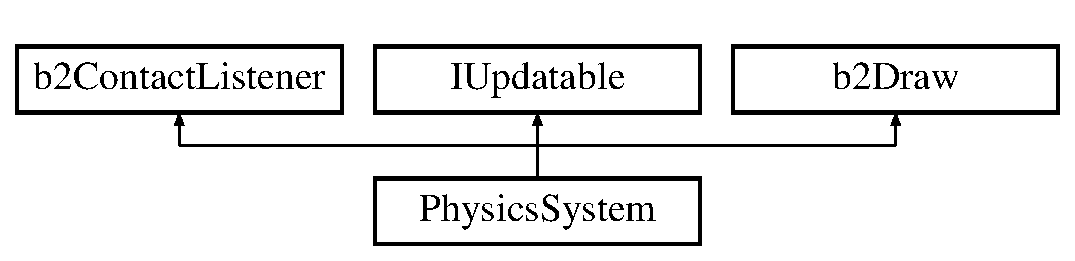
\includegraphics[height=2.000000cm]{class_physics_system}
\end{center}
\end{figure}
\subsection*{Public Types}
\begin{DoxyCompactItemize}
\item 
\mbox{\Hypertarget{class_physics_system_aa9b3a5f5c38063cdc3a78717250a239e}\label{class_physics_system_aa9b3a5f5c38063cdc3a78717250a239e}} 
enum \mbox{\hyperlink{class_physics_system_aa9b3a5f5c38063cdc3a78717250a239e}{Rigid\+Body\+Type}} \{ {\bfseries k\+Static}, 
{\bfseries k\+Dynamic}, 
{\bfseries k\+Num\+Of\+Types}
 \}
\begin{DoxyCompactList}\small\item\em Rigid Body types. \end{DoxyCompactList}\item 
\mbox{\Hypertarget{class_physics_system_ac3b7ef40b19864e4ecdec88af3420a89}\label{class_physics_system_ac3b7ef40b19864e4ecdec88af3420a89}} 
enum \mbox{\hyperlink{class_physics_system_ac3b7ef40b19864e4ecdec88af3420a89}{Polygon\+Shape\+Type}} \{ {\bfseries k\+Box}, 
{\bfseries k\+Num\+Of\+Types}
 \}
\begin{DoxyCompactList}\small\item\em Polygon Shape types. \end{DoxyCompactList}\end{DoxyCompactItemize}
\subsection*{Public Member Functions}
\begin{DoxyCompactItemize}
\item 
void \mbox{\hyperlink{class_physics_system_afa1b487619b6e9e1c16ec03fb9fd4270}{Create\+Physics\+World}} (b2\+Vec2 gravity)
\begin{DoxyCompactList}\small\item\em Creates a physics world. There can only be one physics world! \end{DoxyCompactList}\item 
b2\+Body $\ast$ \mbox{\hyperlink{class_physics_system_a6f1d9c9e9662f641332912172443376e}{Create\+Rigid\+Body}} (b2\+Body\+Def $\ast$p\+Body\+Def)
\begin{DoxyCompactList}\small\item\em Creates a rigid body. This is needed for a world. \end{DoxyCompactList}\item 
\mbox{\Hypertarget{class_physics_system_aabb107eb3795556bff83099d7f3cb710}\label{class_physics_system_aabb107eb3795556bff83099d7f3cb710}} 
virtual void \mbox{\hyperlink{class_physics_system_aabb107eb3795556bff83099d7f3cb710}{Update}} (float delta\+Time\+\_\+sec) override
\begin{DoxyCompactList}\small\item\em Updates the physics world. \end{DoxyCompactList}\item 
b2\+Polygon\+Shape $\ast$ \mbox{\hyperlink{class_physics_system_a651f848a76752bfb3f69e99a3a908865}{Create\+Polygon}} (const \mbox{\hyperlink{class_physics_system_ac3b7ef40b19864e4ecdec88af3420a89}{Polygon\+Shape\+Type}} type, float width, float height)
\begin{DoxyCompactList}\small\item\em Creates and returns a polygon shape. \end{DoxyCompactList}\item 
\mbox{\Hypertarget{class_physics_system_a19f4322c3ffe4c8ba2077dcc638e8039}\label{class_physics_system_a19f4322c3ffe4c8ba2077dcc638e8039}} 
void \mbox{\hyperlink{class_physics_system_a19f4322c3ffe4c8ba2077dcc638e8039}{Cleanup}} ()
\begin{DoxyCompactList}\small\item\em Cleans up the physics system from memory. \end{DoxyCompactList}\item 
\mbox{\Hypertarget{class_physics_system_a294106832fdfe2bc30878a7ed6380fb0}\label{class_physics_system_a294106832fdfe2bc30878a7ed6380fb0}} 
void \mbox{\hyperlink{class_physics_system_a294106832fdfe2bc30878a7ed6380fb0}{Set\+Renderer}} (S\+D\+L\+\_\+\+Renderer $\ast$p\+Renderer)
\begin{DoxyCompactList}\small\item\em Draws physics debug info. \end{DoxyCompactList}\item 
\mbox{\Hypertarget{class_physics_system_a9d09acb7309a9bd0c1527ab8b5e39469}\label{class_physics_system_a9d09acb7309a9bd0c1527ab8b5e39469}} 
void \mbox{\hyperlink{class_physics_system_a9d09acb7309a9bd0c1527ab8b5e39469}{Draw\+Debug\+Info}} ()
\begin{DoxyCompactList}\small\item\em Draws debug info. \end{DoxyCompactList}\item 
\mbox{\Hypertarget{class_physics_system_a3ee533540e81eac532453c4c02c8749a}\label{class_physics_system_a3ee533540e81eac532453c4c02c8749a}} 
virtual void {\bfseries Draw\+Polygon} (const b2\+Vec2 $\ast$vertices, int32 vertex\+Count, const b2\+Color \&color) override
\item 
\mbox{\Hypertarget{class_physics_system_a61db3554729697a2023e297d28c7b958}\label{class_physics_system_a61db3554729697a2023e297d28c7b958}} 
virtual void {\bfseries Draw\+Solid\+Polygon} (const b2\+Vec2 $\ast$vertices, int32 vertex\+Count, const b2\+Color \&color) override
\item 
\mbox{\Hypertarget{class_physics_system_a1c653117bcff772a3d9dc1462c081fc7}\label{class_physics_system_a1c653117bcff772a3d9dc1462c081fc7}} 
virtual void {\bfseries Draw\+Circle} (const b2\+Vec2 \&center, float32 radius, const b2\+Color \&color) override
\item 
\mbox{\Hypertarget{class_physics_system_a6e17da4cb6c33eabee1a4f9276a71598}\label{class_physics_system_a6e17da4cb6c33eabee1a4f9276a71598}} 
virtual void {\bfseries Draw\+Solid\+Circle} (const b2\+Vec2 \&center, float32 radius, const b2\+Vec2 \&axis, const b2\+Color \&color) override
\item 
\mbox{\Hypertarget{class_physics_system_a65d8bb17d93f22cbf0bc54d62dc94ed0}\label{class_physics_system_a65d8bb17d93f22cbf0bc54d62dc94ed0}} 
virtual void {\bfseries Draw\+Segment} (const b2\+Vec2 \&p1, const b2\+Vec2 \&p2, const b2\+Color \&color) override
\item 
\mbox{\Hypertarget{class_physics_system_a5b3cecb4fb81082cb4cf14fc21d91d06}\label{class_physics_system_a5b3cecb4fb81082cb4cf14fc21d91d06}} 
virtual void {\bfseries Draw\+Transform} (const b2\+Transform \&xf) override
\item 
\mbox{\Hypertarget{class_physics_system_a44da913dfdad57c721c2b6330b485081}\label{class_physics_system_a44da913dfdad57c721c2b6330b485081}} 
virtual void {\bfseries Draw\+Point} (const b2\+Vec2 \&p, float32 size, const b2\+Color \&color) override
\end{DoxyCompactItemize}
\subsection*{Static Public Member Functions}
\begin{DoxyCompactItemize}
\item 
\mbox{\Hypertarget{class_physics_system_ad40ddb4eaaa38a223440d98080c1ddfc}\label{class_physics_system_ad40ddb4eaaa38a223440d98080c1ddfc}} 
static \mbox{\hyperlink{class_physics_system}{Physics\+System}} $\ast$ \mbox{\hyperlink{class_physics_system_ad40ddb4eaaa38a223440d98080c1ddfc}{Get}} ()
\begin{DoxyCompactList}\small\item\em Returns an instance of the system. \end{DoxyCompactList}\item 
\mbox{\Hypertarget{class_physics_system_a40db15dde9716172d2ba1d7622a196fd}\label{class_physics_system_a40db15dde9716172d2ba1d7622a196fd}} 
static void \mbox{\hyperlink{class_physics_system_a40db15dde9716172d2ba1d7622a196fd}{Delete}} ()
\begin{DoxyCompactList}\small\item\em Deletes the instance. \end{DoxyCompactList}\end{DoxyCompactItemize}


\subsection{Detailed Description}
Physics system for engine. 

\subsection{Member Function Documentation}
\mbox{\Hypertarget{class_physics_system_afa1b487619b6e9e1c16ec03fb9fd4270}\label{class_physics_system_afa1b487619b6e9e1c16ec03fb9fd4270}} 
\index{Physics\+System@{Physics\+System}!Create\+Physics\+World@{Create\+Physics\+World}}
\index{Create\+Physics\+World@{Create\+Physics\+World}!Physics\+System@{Physics\+System}}
\subsubsection{\texorpdfstring{Create\+Physics\+World()}{CreatePhysicsWorld()}}
{\footnotesize\ttfamily void Physics\+System\+::\+Create\+Physics\+World (\begin{DoxyParamCaption}\item[{b2\+Vec2}]{gravity }\end{DoxyParamCaption})}



Creates a physics world. There can only be one physics world! 


\begin{DoxyParams}{Parameters}
{\em gravity} & Gravity for the world \\
\hline
\end{DoxyParams}
\mbox{\Hypertarget{class_physics_system_a651f848a76752bfb3f69e99a3a908865}\label{class_physics_system_a651f848a76752bfb3f69e99a3a908865}} 
\index{Physics\+System@{Physics\+System}!Create\+Polygon@{Create\+Polygon}}
\index{Create\+Polygon@{Create\+Polygon}!Physics\+System@{Physics\+System}}
\subsubsection{\texorpdfstring{Create\+Polygon()}{CreatePolygon()}}
{\footnotesize\ttfamily b2\+Polygon\+Shape $\ast$ Physics\+System\+::\+Create\+Polygon (\begin{DoxyParamCaption}\item[{const \mbox{\hyperlink{class_physics_system_ac3b7ef40b19864e4ecdec88af3420a89}{Polygon\+Shape\+Type}}}]{type,  }\item[{float}]{width,  }\item[{float}]{height }\end{DoxyParamCaption})}



Creates and returns a polygon shape. 


\begin{DoxyParams}{Parameters}
{\em type} & The type of polygon shape to make \\
\hline
{\em width} & Width of the shape to make \\
\hline
{\em height} & Height of the shape to make \\
\hline
\end{DoxyParams}
\mbox{\Hypertarget{class_physics_system_a6f1d9c9e9662f641332912172443376e}\label{class_physics_system_a6f1d9c9e9662f641332912172443376e}} 
\index{Physics\+System@{Physics\+System}!Create\+Rigid\+Body@{Create\+Rigid\+Body}}
\index{Create\+Rigid\+Body@{Create\+Rigid\+Body}!Physics\+System@{Physics\+System}}
\subsubsection{\texorpdfstring{Create\+Rigid\+Body()}{CreateRigidBody()}}
{\footnotesize\ttfamily b2\+Body $\ast$ Physics\+System\+::\+Create\+Rigid\+Body (\begin{DoxyParamCaption}\item[{b2\+Body\+Def $\ast$}]{p\+Body\+Def }\end{DoxyParamCaption})}



Creates a rigid body. This is needed for a world. 


\begin{DoxyParams}{Parameters}
{\em type} & Type of rigid body to create. \\
\hline
{\em x\+Pos} & X position of rigid body \\
\hline
{\em y\+Pos} & Y position of rigid body \\
\hline
\end{DoxyParams}


The documentation for this class was generated from the following files\+:\begin{DoxyCompactItemize}
\item 
Source/\+Logic/\+Physics/\mbox{\hyperlink{_physics_system_8h}{Physics\+System.\+h}}\item 
Source/\+Logic/\+Physics/Physics\+System.\+cpp\end{DoxyCompactItemize}

\hypertarget{class_resource_system}{}\section{Resource\+System Class Reference}
\label{class_resource_system}\index{Resource\+System@{Resource\+System}}


Overseer of all engine resources.  




{\ttfamily \#include $<$Resource\+System.\+h$>$}

\subsection*{Public Member Functions}
\begin{DoxyCompactItemize}
\item 
\mbox{\hyperlink{class_resource_system_a635cbc11ec235e902cfd689371a3abec}{Resource\+System}} ()=delete
\end{DoxyCompactItemize}
\subsection*{Static Public Member Functions}
\begin{DoxyCompactItemize}
\item 
static void \mbox{\hyperlink{class_resource_system_ac4a4f93f639f85ed01f6482343cf22bf}{Load\+Resource}} (const std\+::string \&name, const std\+::string \&file\+Path, const \mbox{\hyperlink{class_i_resource_a693b751055bf043ebcd424a89831397f}{I\+Resource\+::\+Type}} \&type)
\begin{DoxyCompactList}\small\item\em Loads a resource to resource map. \end{DoxyCompactList}\item 
\mbox{\Hypertarget{class_resource_system_a0c623d474660a64ba10e2ae16697430c}\label{class_resource_system_a0c623d474660a64ba10e2ae16697430c}} 
static void \mbox{\hyperlink{class_resource_system_a0c623d474660a64ba10e2ae16697430c}{Clean\+Up}} ()
\begin{DoxyCompactList}\small\item\em Cleans up the system. \end{DoxyCompactList}\item 
static \mbox{\hyperlink{class_i_resource}{I\+Resource}} $\ast$ \mbox{\hyperlink{class_resource_system_a6cdcecb56a3f7131836b16d2afd10aa7}{Get\+Resource}} (const std\+::string \&name)
\begin{DoxyCompactList}\small\item\em Returns a resource from resource map. \end{DoxyCompactList}\item 
\mbox{\Hypertarget{class_resource_system_ae6b48360c28a728a2e619343ac410505}\label{class_resource_system_ae6b48360c28a728a2e619343ac410505}} 
static void \mbox{\hyperlink{class_resource_system_ae6b48360c28a728a2e619343ac410505}{Set\+Renderer}} (S\+D\+L\+\_\+\+Renderer $\ast$p\+Renderer)
\begin{DoxyCompactList}\small\item\em Sets the renderer to use. \end{DoxyCompactList}\end{DoxyCompactItemize}


\subsection{Detailed Description}
Overseer of all engine resources. 

\subsection{Constructor \& Destructor Documentation}
\mbox{\Hypertarget{class_resource_system_a635cbc11ec235e902cfd689371a3abec}\label{class_resource_system_a635cbc11ec235e902cfd689371a3abec}} 
\index{Resource\+System@{Resource\+System}!Resource\+System@{Resource\+System}}
\index{Resource\+System@{Resource\+System}!Resource\+System@{Resource\+System}}
\subsubsection{\texorpdfstring{Resource\+System()}{ResourceSystem()}}
{\footnotesize\ttfamily Resource\+System\+::\+Resource\+System (\begin{DoxyParamCaption}{ }\end{DoxyParamCaption})\hspace{0.3cm}{\ttfamily [delete]}}

Constructor Not ment to be invoked 

\subsection{Member Function Documentation}
\mbox{\Hypertarget{class_resource_system_a6cdcecb56a3f7131836b16d2afd10aa7}\label{class_resource_system_a6cdcecb56a3f7131836b16d2afd10aa7}} 
\index{Resource\+System@{Resource\+System}!Get\+Resource@{Get\+Resource}}
\index{Get\+Resource@{Get\+Resource}!Resource\+System@{Resource\+System}}
\subsubsection{\texorpdfstring{Get\+Resource()}{GetResource()}}
{\footnotesize\ttfamily static \mbox{\hyperlink{class_i_resource}{I\+Resource}}$\ast$ Resource\+System\+::\+Get\+Resource (\begin{DoxyParamCaption}\item[{const std\+::string \&}]{name }\end{DoxyParamCaption})\hspace{0.3cm}{\ttfamily [inline]}, {\ttfamily [static]}}



Returns a resource from resource map. 


\begin{DoxyParams}{Parameters}
{\em name} & Name of resource to load \\
\hline
\end{DoxyParams}
\mbox{\Hypertarget{class_resource_system_ac4a4f93f639f85ed01f6482343cf22bf}\label{class_resource_system_ac4a4f93f639f85ed01f6482343cf22bf}} 
\index{Resource\+System@{Resource\+System}!Load\+Resource@{Load\+Resource}}
\index{Load\+Resource@{Load\+Resource}!Resource\+System@{Resource\+System}}
\subsubsection{\texorpdfstring{Load\+Resource()}{LoadResource()}}
{\footnotesize\ttfamily void Resource\+System\+::\+Load\+Resource (\begin{DoxyParamCaption}\item[{const std\+::string \&}]{name,  }\item[{const std\+::string \&}]{file\+Path,  }\item[{const \mbox{\hyperlink{class_i_resource_a693b751055bf043ebcd424a89831397f}{I\+Resource\+::\+Type}} \&}]{type }\end{DoxyParamCaption})\hspace{0.3cm}{\ttfamily [static]}}



Loads a resource to resource map. 


\begin{DoxyParams}{Parameters}
{\em name} & Name for to be loaded resource \\
\hline
{\em file\+Path} & resource file to load \\
\hline
{\em type} & Type of resource to load \\
\hline
\end{DoxyParams}


The documentation for this class was generated from the following files\+:\begin{DoxyCompactItemize}
\item 
Source/\+Views/\mbox{\hyperlink{_resource_system_8h}{Resource\+System.\+h}}\item 
Source/\+Views/Resource\+System.\+cpp\end{DoxyCompactItemize}

\hypertarget{class_script_system}{}\section{Script\+System Class Reference}
\label{class_script_system}\index{Script\+System@{Script\+System}}


The documentation for this class was generated from the following files\+:\begin{DoxyCompactItemize}
\item 
Source/\+Logic/\+Scripting/Script\+System.\+h\item 
Source/\+Logic/\+Scripting/Script\+System.\+cpp\end{DoxyCompactItemize}

\hypertarget{struct_sfx_event}{}\section{Sfx\+Event Struct Reference}
\label{struct_sfx_event}\index{Sfx\+Event@{Sfx\+Event}}


Structure for Sfx Events.  




{\ttfamily \#include $<$Event\+System.\+h$>$}

Inheritance diagram for Sfx\+Event\+:\begin{figure}[H]
\begin{center}
\leavevmode
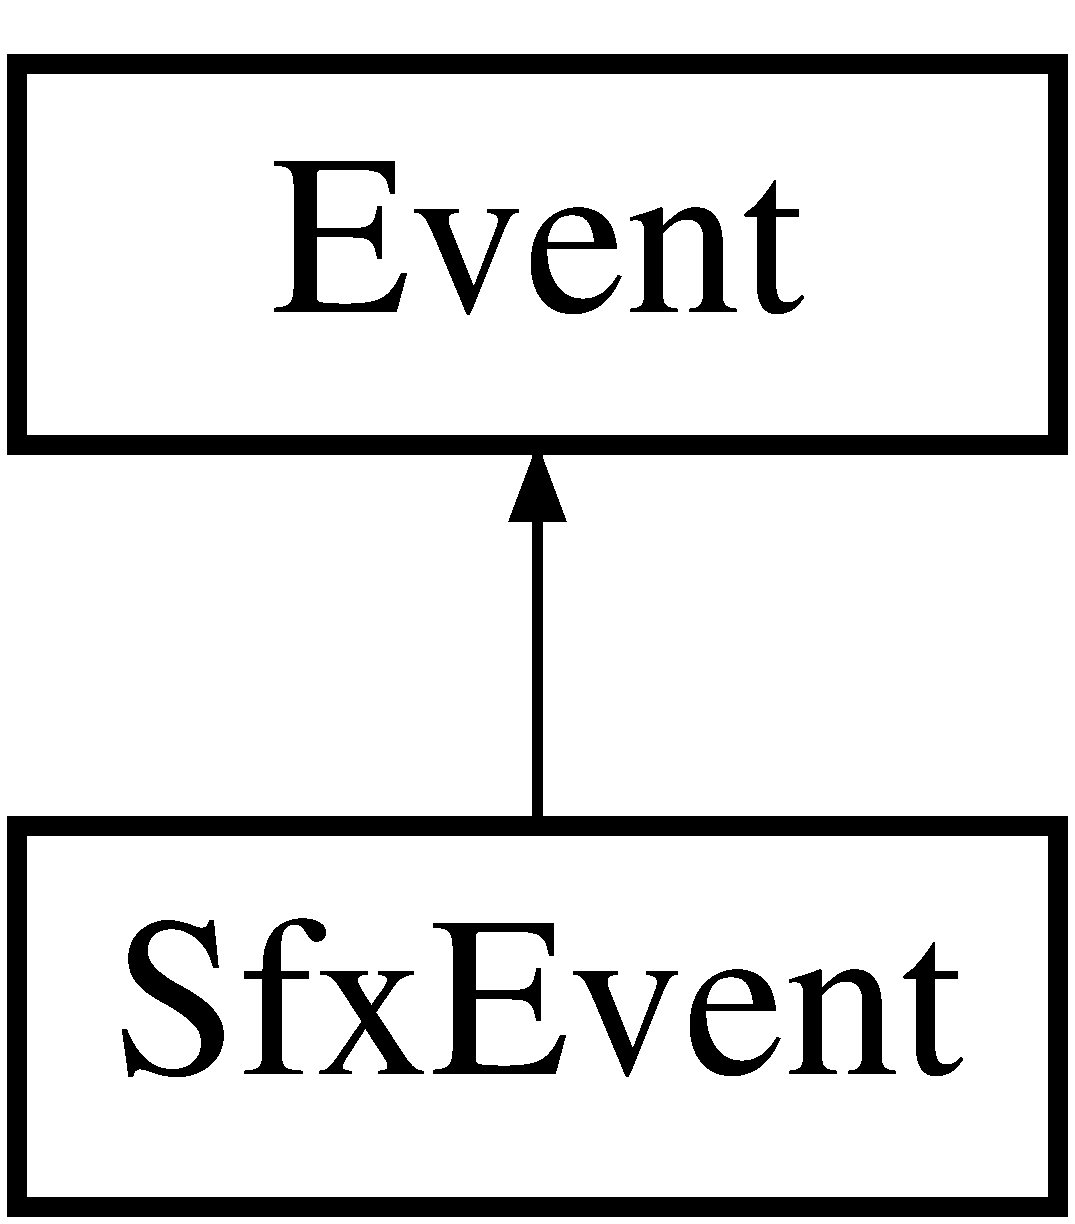
\includegraphics[height=2.000000cm]{struct_sfx_event}
\end{center}
\end{figure}
\subsection*{Public Attributes}
\begin{DoxyCompactItemize}
\item 
\mbox{\Hypertarget{struct_sfx_event_a1c70334abf08d52d4916b345b80df8e5}\label{struct_sfx_event_a1c70334abf08d52d4916b345b80df8e5}} 
std\+::string \mbox{\hyperlink{struct_sfx_event_a1c70334abf08d52d4916b345b80df8e5}{m\+\_\+sfx\+Name}}
\begin{DoxyCompactList}\small\item\em Name of the sfx. \end{DoxyCompactList}\item 
\mbox{\Hypertarget{struct_sfx_event_a8fa9bf1c45b7deeb673b0d161f92bd7a}\label{struct_sfx_event_a8fa9bf1c45b7deeb673b0d161f92bd7a}} 
std\+::string \mbox{\hyperlink{struct_sfx_event_a8fa9bf1c45b7deeb673b0d161f92bd7a}{m\+\_\+sfx\+File}}
\begin{DoxyCompactList}\small\item\em Filename for the sfx. \end{DoxyCompactList}\end{DoxyCompactItemize}
\subsection*{Additional Inherited Members}


\subsection{Detailed Description}
Structure for Sfx Events. 

The documentation for this struct was generated from the following file\+:\begin{DoxyCompactItemize}
\item 
Source/\+Logic/\+Events/\mbox{\hyperlink{_event_system_8h}{Event\+System.\+h}}\end{DoxyCompactItemize}

\hypertarget{struct_sfx_resource}{}\section{Sfx\+Resource Struct Reference}
\label{struct_sfx_resource}\index{Sfx\+Resource@{Sfx\+Resource}}


Represents a Sfx resource.  




{\ttfamily \#include $<$Resource\+System.\+h$>$}

Inheritance diagram for Sfx\+Resource\+:\begin{figure}[H]
\begin{center}
\leavevmode
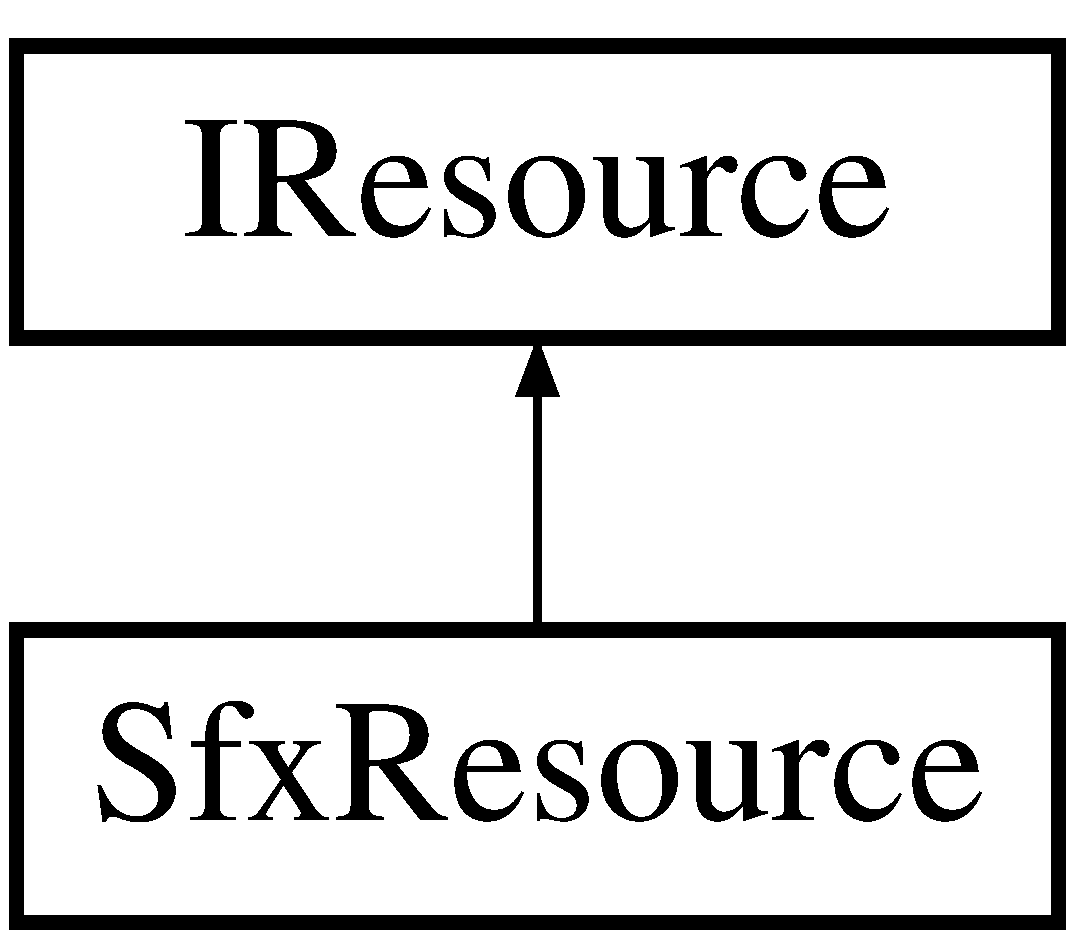
\includegraphics[height=2.000000cm]{struct_sfx_resource}
\end{center}
\end{figure}
\subsection*{Public Attributes}
\begin{DoxyCompactItemize}
\item 
\mbox{\Hypertarget{struct_sfx_resource_a5f29af4667386c5619c994a824a5efb2}\label{struct_sfx_resource_a5f29af4667386c5619c994a824a5efb2}} 
Mix\+\_\+\+Chunk $\ast$ \mbox{\hyperlink{struct_sfx_resource_a5f29af4667386c5619c994a824a5efb2}{m\+\_\+p\+Sfx}}
\begin{DoxyCompactList}\small\item\em Sfx this resource represents. \end{DoxyCompactList}\end{DoxyCompactItemize}
\subsection*{Additional Inherited Members}


\subsection{Detailed Description}
Represents a Sfx resource. 

The documentation for this struct was generated from the following file\+:\begin{DoxyCompactItemize}
\item 
Source/\+Views/\mbox{\hyperlink{_resource_system_8h}{Resource\+System.\+h}}\end{DoxyCompactItemize}

\hypertarget{classtinyxml2_1_1_str_pair}{}\section{tinyxml2\+:\+:Str\+Pair Class Reference}
\label{classtinyxml2_1_1_str_pair}\index{tinyxml2\+::\+Str\+Pair@{tinyxml2\+::\+Str\+Pair}}
\subsection*{Public Types}
\begin{DoxyCompactItemize}
\item 
\mbox{\Hypertarget{classtinyxml2_1_1_str_pair_a0301ef962e15dd94574431f1c61266c5}\label{classtinyxml2_1_1_str_pair_a0301ef962e15dd94574431f1c61266c5}} 
enum \{ \newline
{\bfseries N\+E\+E\+D\+S\+\_\+\+E\+N\+T\+I\+T\+Y\+\_\+\+P\+R\+O\+C\+E\+S\+S\+I\+NG} = 0x01, 
{\bfseries N\+E\+E\+D\+S\+\_\+\+N\+E\+W\+L\+I\+N\+E\+\_\+\+N\+O\+R\+M\+A\+L\+I\+Z\+A\+T\+I\+ON} = 0x02, 
{\bfseries N\+E\+E\+D\+S\+\_\+\+W\+H\+I\+T\+E\+S\+P\+A\+C\+E\+\_\+\+C\+O\+L\+L\+A\+P\+S\+I\+NG} = 0x04, 
{\bfseries T\+E\+X\+T\+\_\+\+E\+L\+E\+M\+E\+NT} = N\+E\+E\+D\+S\+\_\+\+E\+N\+T\+I\+T\+Y\+\_\+\+P\+R\+O\+C\+E\+S\+S\+I\+NG $\vert$ N\+E\+E\+D\+S\+\_\+\+N\+E\+W\+L\+I\+N\+E\+\_\+\+N\+O\+R\+M\+A\+L\+I\+Z\+A\+T\+I\+ON, 
\newline
{\bfseries T\+E\+X\+T\+\_\+\+E\+L\+E\+M\+E\+N\+T\+\_\+\+L\+E\+A\+V\+E\+\_\+\+E\+N\+T\+I\+T\+I\+ES} = N\+E\+E\+D\+S\+\_\+\+N\+E\+W\+L\+I\+N\+E\+\_\+\+N\+O\+R\+M\+A\+L\+I\+Z\+A\+T\+I\+ON, 
{\bfseries A\+T\+T\+R\+I\+B\+U\+T\+E\+\_\+\+N\+A\+ME} = 0, 
{\bfseries A\+T\+T\+R\+I\+B\+U\+T\+E\+\_\+\+V\+A\+L\+UE} = N\+E\+E\+D\+S\+\_\+\+E\+N\+T\+I\+T\+Y\+\_\+\+P\+R\+O\+C\+E\+S\+S\+I\+NG $\vert$ N\+E\+E\+D\+S\+\_\+\+N\+E\+W\+L\+I\+N\+E\+\_\+\+N\+O\+R\+M\+A\+L\+I\+Z\+A\+T\+I\+ON, 
{\bfseries A\+T\+T\+R\+I\+B\+U\+T\+E\+\_\+\+V\+A\+L\+U\+E\+\_\+\+L\+E\+A\+V\+E\+\_\+\+E\+N\+T\+I\+T\+I\+ES} = N\+E\+E\+D\+S\+\_\+\+N\+E\+W\+L\+I\+N\+E\+\_\+\+N\+O\+R\+M\+A\+L\+I\+Z\+A\+T\+I\+ON, 
\newline
{\bfseries C\+O\+M\+M\+E\+NT} = N\+E\+E\+D\+S\+\_\+\+N\+E\+W\+L\+I\+N\+E\+\_\+\+N\+O\+R\+M\+A\+L\+I\+Z\+A\+T\+I\+ON
 \}
\end{DoxyCompactItemize}
\subsection*{Public Member Functions}
\begin{DoxyCompactItemize}
\item 
\mbox{\Hypertarget{classtinyxml2_1_1_str_pair_a4f05549373394266a1eecba26813c166}\label{classtinyxml2_1_1_str_pair_a4f05549373394266a1eecba26813c166}} 
void {\bfseries Set} (char $\ast$start, char $\ast$end, int flags)
\item 
\mbox{\Hypertarget{classtinyxml2_1_1_str_pair_ad87e3d11330f5e689ba1e7e54c023b57}\label{classtinyxml2_1_1_str_pair_ad87e3d11330f5e689ba1e7e54c023b57}} 
const char $\ast$ {\bfseries Get\+Str} ()
\item 
\mbox{\Hypertarget{classtinyxml2_1_1_str_pair_aca963a7eaa900bfddbea7312f040b39c}\label{classtinyxml2_1_1_str_pair_aca963a7eaa900bfddbea7312f040b39c}} 
bool {\bfseries Empty} () const
\item 
\mbox{\Hypertarget{classtinyxml2_1_1_str_pair_a2baf6230e18333e02ab65d0897ee3941}\label{classtinyxml2_1_1_str_pair_a2baf6230e18333e02ab65d0897ee3941}} 
void {\bfseries Set\+Interned\+Str} (const char $\ast$str)
\item 
\mbox{\Hypertarget{classtinyxml2_1_1_str_pair_a1f82ec6b5bee35ee7466d8565e43b1de}\label{classtinyxml2_1_1_str_pair_a1f82ec6b5bee35ee7466d8565e43b1de}} 
void {\bfseries Set\+Str} (const char $\ast$str, int flags=0)
\item 
\mbox{\Hypertarget{classtinyxml2_1_1_str_pair_a68e6999b7677fa711287ececb9ba317e}\label{classtinyxml2_1_1_str_pair_a68e6999b7677fa711287ececb9ba317e}} 
char $\ast$ {\bfseries Parse\+Text} (char $\ast$in, const char $\ast$end\+Tag, int str\+Flags, int $\ast$cur\+Line\+Num\+Ptr)
\item 
\mbox{\Hypertarget{classtinyxml2_1_1_str_pair_aa6d8998efceba41d87ec2300c70a6085}\label{classtinyxml2_1_1_str_pair_aa6d8998efceba41d87ec2300c70a6085}} 
char $\ast$ {\bfseries Parse\+Name} (char $\ast$in)
\item 
\mbox{\Hypertarget{classtinyxml2_1_1_str_pair_a35f795b1557fe5fdcbd93d3cc5d6b939}\label{classtinyxml2_1_1_str_pair_a35f795b1557fe5fdcbd93d3cc5d6b939}} 
void {\bfseries Transfer\+To} (\mbox{\hyperlink{classtinyxml2_1_1_str_pair}{Str\+Pair}} $\ast$other)
\item 
\mbox{\Hypertarget{classtinyxml2_1_1_str_pair_a80c1b3bd99bf62ae85c94a29ce537125}\label{classtinyxml2_1_1_str_pair_a80c1b3bd99bf62ae85c94a29ce537125}} 
void {\bfseries Reset} ()
\end{DoxyCompactItemize}


The documentation for this class was generated from the following files\+:\begin{DoxyCompactItemize}
\item 
Source/\+Utils/tinyxml2.\+h\item 
Source/\+Utils/tinyxml2.\+cpp\end{DoxyCompactItemize}

\hypertarget{struct_texture_component}{}\section{Texture\+Component Struct Reference}
\label{struct_texture_component}\index{Texture\+Component@{Texture\+Component}}


Structure to store texture data.  




{\ttfamily \#include $<$Texture\+Component.\+h$>$}

Inheritance diagram for Texture\+Component\+:\begin{figure}[H]
\begin{center}
\leavevmode
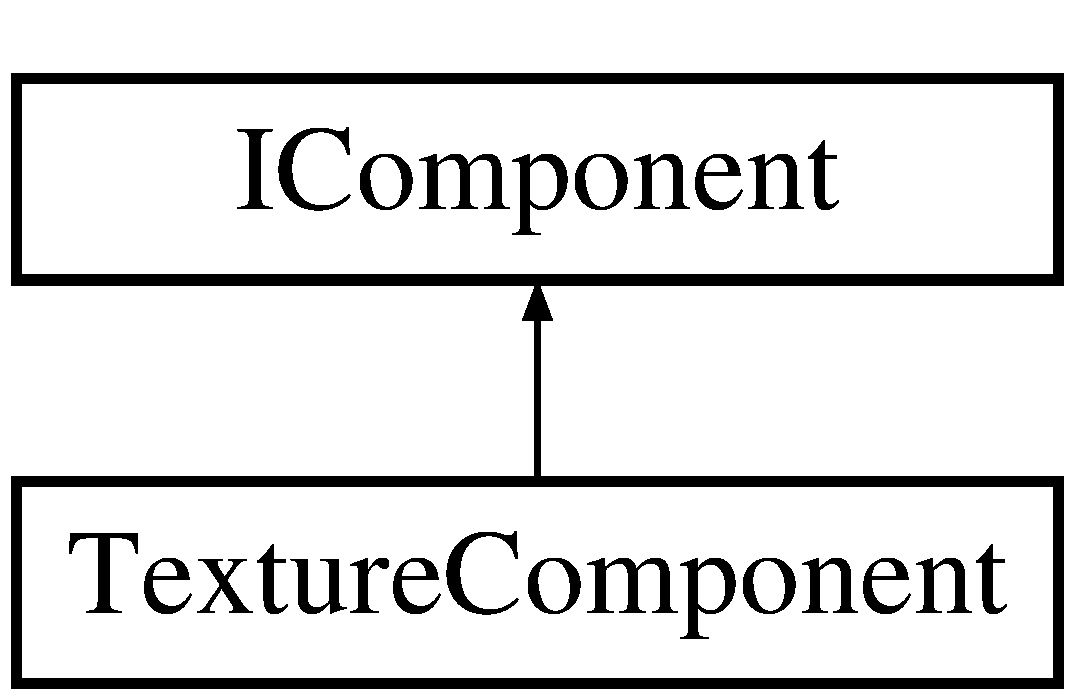
\includegraphics[height=2.000000cm]{struct_texture_component}
\end{center}
\end{figure}
\subsection*{Public Attributes}
\begin{DoxyCompactItemize}
\item 
\mbox{\Hypertarget{struct_texture_component_acb41794a83d0a9b43015e8c979bc988c}\label{struct_texture_component_acb41794a83d0a9b43015e8c979bc988c}} 
std\+::string \mbox{\hyperlink{struct_texture_component_acb41794a83d0a9b43015e8c979bc988c}{m\+\_\+name}}
\begin{DoxyCompactList}\small\item\em Texture name. \end{DoxyCompactList}\item 
\mbox{\Hypertarget{struct_texture_component_a7ed9b861446b42f3fa02532e2af227a0}\label{struct_texture_component_a7ed9b861446b42f3fa02532e2af227a0}} 
S\+D\+L\+\_\+\+Texture $\ast$ \mbox{\hyperlink{struct_texture_component_a7ed9b861446b42f3fa02532e2af227a0}{m\+\_\+p\+Texture}}
\begin{DoxyCompactList}\small\item\em Texture data. \end{DoxyCompactList}\item 
\mbox{\Hypertarget{struct_texture_component_ab490306423d90975c8dae0ef565bd60a}\label{struct_texture_component_ab490306423d90975c8dae0ef565bd60a}} 
S\+D\+L\+\_\+\+Rect \mbox{\hyperlink{struct_texture_component_ab490306423d90975c8dae0ef565bd60a}{m\+\_\+src\+Rect}}
\begin{DoxyCompactList}\small\item\em Source rect for textures. \end{DoxyCompactList}\end{DoxyCompactItemize}
\subsection*{Additional Inherited Members}


\subsection{Detailed Description}
Structure to store texture data. 

The documentation for this struct was generated from the following file\+:\begin{DoxyCompactItemize}
\item 
Source/\+Logic/\+Game\+Objects/\mbox{\hyperlink{_texture_component_8h}{Texture\+Component.\+h}}\end{DoxyCompactItemize}

\hypertarget{struct_texture_event}{}\section{Texture\+Event Struct Reference}
\label{struct_texture_event}\index{Texture\+Event@{Texture\+Event}}


Structure for Texture events.  




{\ttfamily \#include $<$Event\+System.\+h$>$}

Inheritance diagram for Texture\+Event\+:\begin{figure}[H]
\begin{center}
\leavevmode
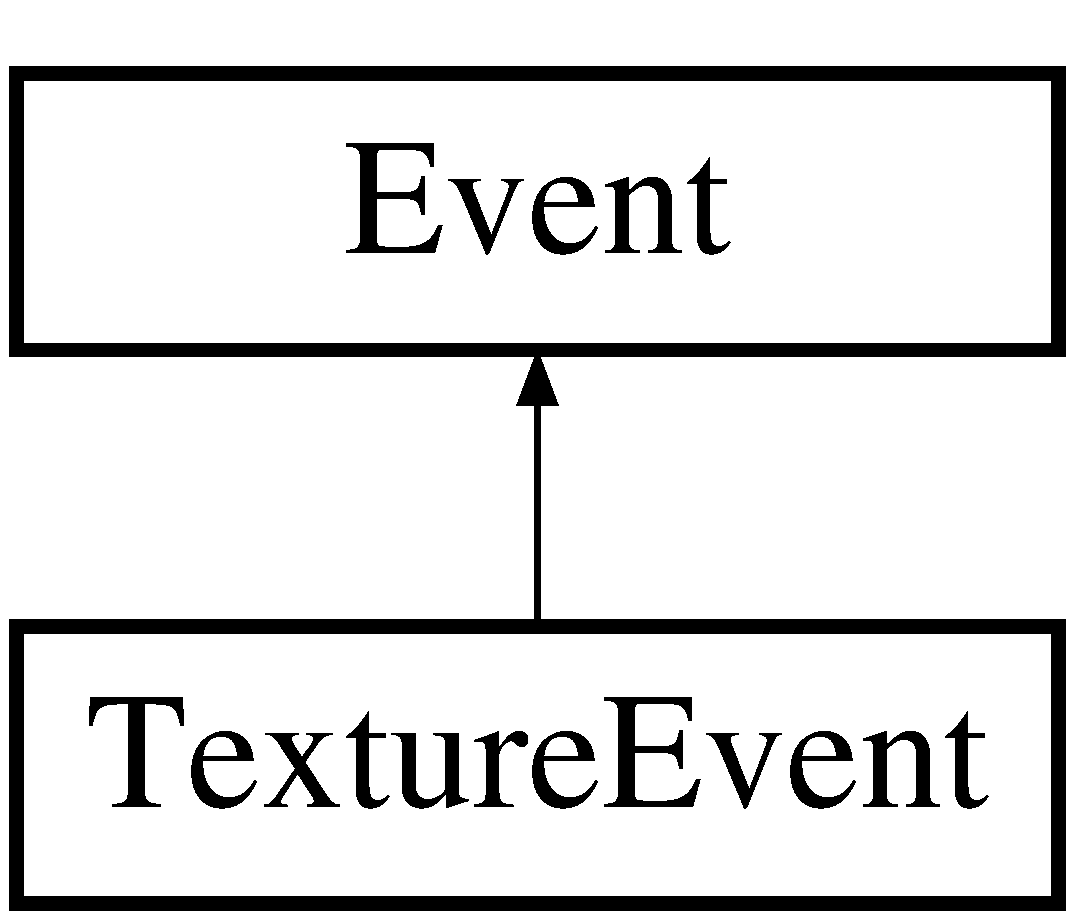
\includegraphics[height=2.000000cm]{struct_texture_event}
\end{center}
\end{figure}
\subsection*{Public Attributes}
\begin{DoxyCompactItemize}
\item 
\mbox{\Hypertarget{struct_texture_event_afa021414f511cb7cdc7d6a2b0ac11a11}\label{struct_texture_event_afa021414f511cb7cdc7d6a2b0ac11a11}} 
std\+::string \mbox{\hyperlink{struct_texture_event_afa021414f511cb7cdc7d6a2b0ac11a11}{m\+\_\+texture\+Name}}
\begin{DoxyCompactList}\small\item\em Name of the texture. \end{DoxyCompactList}\item 
\mbox{\Hypertarget{struct_texture_event_a7233f36930918ea417d2a7eeb2c42be2}\label{struct_texture_event_a7233f36930918ea417d2a7eeb2c42be2}} 
std\+::string \mbox{\hyperlink{struct_texture_event_a7233f36930918ea417d2a7eeb2c42be2}{m\+\_\+texture\+File}}
\begin{DoxyCompactList}\small\item\em Filename for the texture. \end{DoxyCompactList}\item 
\mbox{\Hypertarget{struct_texture_event_ae5935726537c85a83447eb527e8a59a1}\label{struct_texture_event_ae5935726537c85a83447eb527e8a59a1}} 
S\+D\+L\+\_\+\+Texture $\ast$ \mbox{\hyperlink{struct_texture_event_ae5935726537c85a83447eb527e8a59a1}{m\+\_\+p\+Texture}}
\begin{DoxyCompactList}\small\item\em The texture data. \end{DoxyCompactList}\end{DoxyCompactItemize}
\subsection*{Additional Inherited Members}


\subsection{Detailed Description}
Structure for Texture events. 

The documentation for this struct was generated from the following file\+:\begin{DoxyCompactItemize}
\item 
Source/\+Logic/\+Events/\mbox{\hyperlink{_event_system_8h}{Event\+System.\+h}}\end{DoxyCompactItemize}

\hypertarget{struct_texture_resource}{}\section{Texture\+Resource Struct Reference}
\label{struct_texture_resource}\index{Texture\+Resource@{Texture\+Resource}}


Represents a texture resource.  




{\ttfamily \#include $<$Resource\+System.\+h$>$}

Inheritance diagram for Texture\+Resource\+:\begin{figure}[H]
\begin{center}
\leavevmode
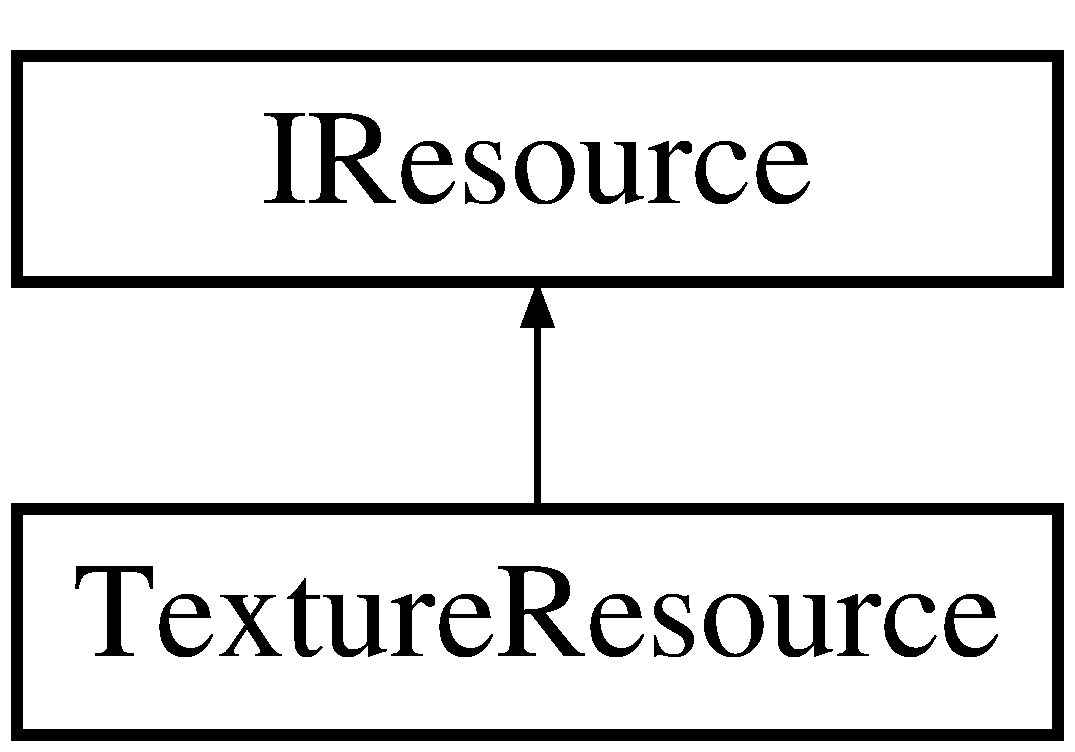
\includegraphics[height=2.000000cm]{struct_texture_resource}
\end{center}
\end{figure}
\subsection*{Public Attributes}
\begin{DoxyCompactItemize}
\item 
\mbox{\Hypertarget{struct_texture_resource_a50412396bd47d075ee020737fa4a9cf2}\label{struct_texture_resource_a50412396bd47d075ee020737fa4a9cf2}} 
S\+D\+L\+\_\+\+Texture $\ast$ \mbox{\hyperlink{struct_texture_resource_a50412396bd47d075ee020737fa4a9cf2}{m\+\_\+p\+Texture}}
\begin{DoxyCompactList}\small\item\em Texture this resource represents. \end{DoxyCompactList}\end{DoxyCompactItemize}
\subsection*{Additional Inherited Members}


\subsection{Detailed Description}
Represents a texture resource. 

The documentation for this struct was generated from the following file\+:\begin{DoxyCompactItemize}
\item 
Source/\+Views/\mbox{\hyperlink{_resource_system_8h}{Resource\+System.\+h}}\end{DoxyCompactItemize}

\hypertarget{struct_vector2_d}{}\section{Vector2D Struct Reference}
\label{struct_vector2_d}\index{Vector2D@{Vector2D}}


Represents 2D vectors in game space.  




{\ttfamily \#include $<$Vector2\+D.\+h$>$}

\subsection*{Public Member Functions}
\begin{DoxyCompactItemize}
\item 
\mbox{\Hypertarget{struct_vector2_d_a8efc0645c81ad58c9bd4bc6143343164}\label{struct_vector2_d_a8efc0645c81ad58c9bd4bc6143343164}} 
\mbox{\hyperlink{struct_vector2_d}{Vector2D}} {\bfseries operator+} (const \mbox{\hyperlink{struct_vector2_d}{Vector2D}} \&v1)
\item 
\mbox{\Hypertarget{struct_vector2_d_a135c4267d27d7b463de8d402ba5818a5}\label{struct_vector2_d_a135c4267d27d7b463de8d402ba5818a5}} 
\mbox{\hyperlink{struct_vector2_d}{Vector2D}} {\bfseries operator-\/} (const \mbox{\hyperlink{struct_vector2_d}{Vector2D}} \&v1)
\item 
\mbox{\Hypertarget{struct_vector2_d_a8ab57bed4f60dad5d083e8b8e833b61f}\label{struct_vector2_d_a8ab57bed4f60dad5d083e8b8e833b61f}} 
\mbox{\hyperlink{struct_vector2_d}{Vector2D}} {\bfseries operator$\ast$} (const \mbox{\hyperlink{struct_vector2_d}{Vector2D}} \&v1)
\item 
\mbox{\Hypertarget{struct_vector2_d_af7e138a171dfd8dff3cb74a63a8acd56}\label{struct_vector2_d_af7e138a171dfd8dff3cb74a63a8acd56}} 
\mbox{\hyperlink{struct_vector2_d}{Vector2D}} {\bfseries operator$\ast$} (float n)
\item 
\mbox{\Hypertarget{struct_vector2_d_ad52aa5d47895dc94d423d469bd0a7a87}\label{struct_vector2_d_ad52aa5d47895dc94d423d469bd0a7a87}} 
\mbox{\hyperlink{struct_vector2_d}{Vector2D}} {\bfseries operator/} (float n)
\item 
\mbox{\Hypertarget{struct_vector2_d_ab726c203370e88dd55a07dc8d1bc55a9}\label{struct_vector2_d_ab726c203370e88dd55a07dc8d1bc55a9}} 
\mbox{\hyperlink{struct_vector2_d}{Vector2D}} {\bfseries operator/} (const \mbox{\hyperlink{struct_vector2_d}{Vector2D}} \&v1)
\item 
\mbox{\Hypertarget{struct_vector2_d_a4382e9f5d04464d8509e0eba8ac23815}\label{struct_vector2_d_a4382e9f5d04464d8509e0eba8ac23815}} 
void {\bfseries operator=} (const \mbox{\hyperlink{struct_vector2_d}{Vector2D}} \&v1)
\item 
\mbox{\Hypertarget{struct_vector2_d_aa01d3728137517fa673770002216f06d}\label{struct_vector2_d_aa01d3728137517fa673770002216f06d}} 
void {\bfseries operator+=} (const \mbox{\hyperlink{struct_vector2_d}{Vector2D}} \&v1)
\item 
\mbox{\Hypertarget{struct_vector2_d_ae49b62b11f190acb45b5e1952c7b9983}\label{struct_vector2_d_ae49b62b11f190acb45b5e1952c7b9983}} 
void {\bfseries operator-\/=} (const \mbox{\hyperlink{struct_vector2_d}{Vector2D}} \&v1)
\item 
\mbox{\Hypertarget{struct_vector2_d_a7050f383416e3be2615e53deecb0abbe}\label{struct_vector2_d_a7050f383416e3be2615e53deecb0abbe}} 
void {\bfseries operator$\ast$=} (const \mbox{\hyperlink{struct_vector2_d}{Vector2D}} \&v1)
\item 
\mbox{\Hypertarget{struct_vector2_d_a2ca66bd619d9c3dc9efefcbefec3e237}\label{struct_vector2_d_a2ca66bd619d9c3dc9efefcbefec3e237}} 
void {\bfseries operator/=} (const \mbox{\hyperlink{struct_vector2_d}{Vector2D}} \&v1)
\item 
\mbox{\Hypertarget{struct_vector2_d_a78830ad34fd3ffa10c4b80c709bd8e40}\label{struct_vector2_d_a78830ad34fd3ffa10c4b80c709bd8e40}} 
bool {\bfseries operator!=} (const \mbox{\hyperlink{struct_vector2_d}{Vector2D}} \&v1)
\item 
\mbox{\Hypertarget{struct_vector2_d_ae26660591b00d7a379869ba0794d00a9}\label{struct_vector2_d_ae26660591b00d7a379869ba0794d00a9}} 
bool {\bfseries operator==} (const \mbox{\hyperlink{struct_vector2_d}{Vector2D}} \&v1)
\end{DoxyCompactItemize}
\subsection*{Public Attributes}
\begin{DoxyCompactItemize}
\item 
\mbox{\Hypertarget{struct_vector2_d_aeba78e197a8ba61f5728cd12710a260b}\label{struct_vector2_d_aeba78e197a8ba61f5728cd12710a260b}} 
float \mbox{\hyperlink{struct_vector2_d_aeba78e197a8ba61f5728cd12710a260b}{m\+\_\+x}}
\begin{DoxyCompactList}\small\item\em X value of vector. \end{DoxyCompactList}\item 
\mbox{\Hypertarget{struct_vector2_d_a2dae7f715b79bbec5470161f6061d13b}\label{struct_vector2_d_a2dae7f715b79bbec5470161f6061d13b}} 
float \mbox{\hyperlink{struct_vector2_d_a2dae7f715b79bbec5470161f6061d13b}{m\+\_\+y}}
\begin{DoxyCompactList}\small\item\em Y value of vector. \end{DoxyCompactList}\item 
\mbox{\Hypertarget{struct_vector2_d_acaa3e890f9b83f6899dad86b3848e719}\label{struct_vector2_d_acaa3e890f9b83f6899dad86b3848e719}} 
float \mbox{\hyperlink{struct_vector2_d_acaa3e890f9b83f6899dad86b3848e719}{m\+\_\+size}}
\begin{DoxyCompactList}\small\item\em Size of vector for normalization purposes. \end{DoxyCompactList}\end{DoxyCompactItemize}


\subsection{Detailed Description}
Represents 2D vectors in game space. 

The documentation for this struct was generated from the following files\+:\begin{DoxyCompactItemize}
\item 
Source/\+Logic/\+Math/\mbox{\hyperlink{_vector2_d_8h}{Vector2\+D.\+h}}\item 
Source/\+Logic/\+Math/Vector2\+D.\+cpp\end{DoxyCompactItemize}

\hypertarget{class_view}{}\section{View Class Reference}
\label{class_view}\index{View@{View}}


Handles display\textquotesingle{}s and sounds of game.  




{\ttfamily \#include $<$View.\+h$>$}

Inheritance diagram for View\+:\begin{figure}[H]
\begin{center}
\leavevmode
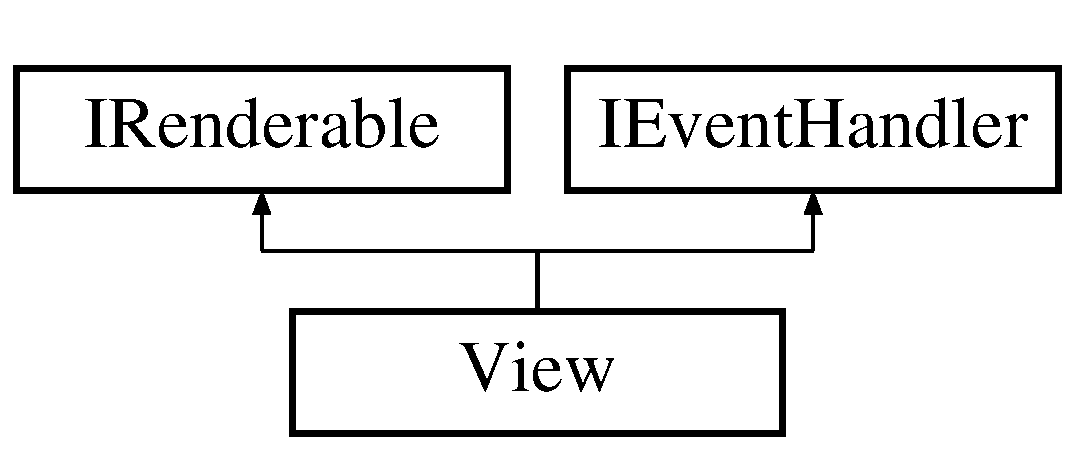
\includegraphics[height=2.000000cm]{class_view}
\end{center}
\end{figure}
\subsection*{Public Member Functions}
\begin{DoxyCompactItemize}
\item 
bool \mbox{\hyperlink{class_view_a721fe641411d670c3679ee6e188c0084}{Init}} (S\+D\+L\+\_\+\+Renderer $\ast$p\+Renderer)
\begin{DoxyCompactList}\small\item\em Initializes the view. \end{DoxyCompactList}\item 
\mbox{\Hypertarget{class_view_a50f75e10ba08bf35196cd71c0b883331}\label{class_view_a50f75e10ba08bf35196cd71c0b883331}} 
void \mbox{\hyperlink{class_view_a50f75e10ba08bf35196cd71c0b883331}{Clean\+Up}} ()
\begin{DoxyCompactList}\small\item\em Cleans up view. \end{DoxyCompactList}\item 
\mbox{\Hypertarget{class_view_acc8397285a5d338f862e6864602e2d87}\label{class_view_acc8397285a5d338f862e6864602e2d87}} 
virtual \mbox{\hyperlink{_macros_8h_a9ce0e6835f82908079752fa4ebe70dc9}{P\+H\+A\+Z\+E\+\_\+\+A\+PI}} void \mbox{\hyperlink{class_view_acc8397285a5d338f862e6864602e2d87}{Render}} () override
\begin{DoxyCompactList}\small\item\em Renders the game. \end{DoxyCompactList}\item 
\mbox{\Hypertarget{class_view_abaeae948fb2fbc2585756afc6962b66e}\label{class_view_abaeae948fb2fbc2585756afc6962b66e}} 
virtual \mbox{\hyperlink{_macros_8h_a9ce0e6835f82908079752fa4ebe70dc9}{P\+H\+A\+Z\+E\+\_\+\+A\+PI}} void \mbox{\hyperlink{class_view_abaeae948fb2fbc2585756afc6962b66e}{Handle\+Event}} (\mbox{\hyperlink{struct_event}{Event}} $\ast$p\+Event) override
\begin{DoxyCompactList}\small\item\em Hanldes an event. \end{DoxyCompactList}\item 
const bool \mbox{\hyperlink{class_view_a899a25e7a81c52ab1ce48ce7675f06df}{Get\+Init\+Flag}} ()
\begin{DoxyCompactList}\small\item\em Returns the initialization flag. \end{DoxyCompactList}\end{DoxyCompactItemize}


\subsection{Detailed Description}
Handles display\textquotesingle{}s and sounds of game. 

\subsection{Member Function Documentation}
\mbox{\Hypertarget{class_view_a899a25e7a81c52ab1ce48ce7675f06df}\label{class_view_a899a25e7a81c52ab1ce48ce7675f06df}} 
\index{View@{View}!Get\+Init\+Flag@{Get\+Init\+Flag}}
\index{Get\+Init\+Flag@{Get\+Init\+Flag}!View@{View}}
\subsubsection{\texorpdfstring{Get\+Init\+Flag()}{GetInitFlag()}}
{\footnotesize\ttfamily const bool View\+::\+Get\+Init\+Flag (\begin{DoxyParamCaption}{ }\end{DoxyParamCaption})\hspace{0.3cm}{\ttfamily [inline]}}



Returns the initialization flag. 

\begin{DoxyReturn}{Returns}
True or False if initialized 
\end{DoxyReturn}
\mbox{\Hypertarget{class_view_a721fe641411d670c3679ee6e188c0084}\label{class_view_a721fe641411d670c3679ee6e188c0084}} 
\index{View@{View}!Init@{Init}}
\index{Init@{Init}!View@{View}}
\subsubsection{\texorpdfstring{Init()}{Init()}}
{\footnotesize\ttfamily bool View\+::\+Init (\begin{DoxyParamCaption}\item[{S\+D\+L\+\_\+\+Renderer $\ast$}]{p\+Renderer }\end{DoxyParamCaption})}



Initializes the view. 


\begin{DoxyParams}{Parameters}
{\em p\+Game} & \mbox{\hyperlink{class_game}{Game}} delegate to render \\
\hline
{\em p\+Renderer} & S\+DL renderer to use \\
\hline
\end{DoxyParams}


The documentation for this class was generated from the following files\+:\begin{DoxyCompactItemize}
\item 
Source/\+Views/\mbox{\hyperlink{_view_8h}{View.\+h}}\item 
Source/\+Views/View.\+cpp\end{DoxyCompactItemize}

\hypertarget{classtinyxml2_1_1_x_m_l_attribute}{}\section{tinyxml2\+:\+:X\+M\+L\+Attribute Class Reference}
\label{classtinyxml2_1_1_x_m_l_attribute}\index{tinyxml2\+::\+X\+M\+L\+Attribute@{tinyxml2\+::\+X\+M\+L\+Attribute}}


{\ttfamily \#include $<$tinyxml2.\+h$>$}

\subsection*{Public Member Functions}
\begin{DoxyCompactItemize}
\item 
\mbox{\Hypertarget{classtinyxml2_1_1_x_m_l_attribute_a5a5c135d24cce7abda6f17301c6274d8}\label{classtinyxml2_1_1_x_m_l_attribute_a5a5c135d24cce7abda6f17301c6274d8}} 
const char $\ast$ \mbox{\hyperlink{classtinyxml2_1_1_x_m_l_attribute_a5a5c135d24cce7abda6f17301c6274d8}{Name}} () const
\begin{DoxyCompactList}\small\item\em The name of the attribute. \end{DoxyCompactList}\item 
\mbox{\Hypertarget{classtinyxml2_1_1_x_m_l_attribute_ab1c5cd993f836a771818ca408994b14e}\label{classtinyxml2_1_1_x_m_l_attribute_ab1c5cd993f836a771818ca408994b14e}} 
const char $\ast$ \mbox{\hyperlink{classtinyxml2_1_1_x_m_l_attribute_ab1c5cd993f836a771818ca408994b14e}{Value}} () const
\begin{DoxyCompactList}\small\item\em The value of the attribute. \end{DoxyCompactList}\item 
\mbox{\Hypertarget{classtinyxml2_1_1_x_m_l_attribute_a02d5ea924586e35f9c13857d1671b765}\label{classtinyxml2_1_1_x_m_l_attribute_a02d5ea924586e35f9c13857d1671b765}} 
int \mbox{\hyperlink{classtinyxml2_1_1_x_m_l_attribute_a02d5ea924586e35f9c13857d1671b765}{Get\+Line\+Num}} () const
\begin{DoxyCompactList}\small\item\em Gets the line number the attribute is in, if the document was parsed from a file. \end{DoxyCompactList}\item 
\mbox{\Hypertarget{classtinyxml2_1_1_x_m_l_attribute_aee53571b21e7ce5421eb929523a8bbe6}\label{classtinyxml2_1_1_x_m_l_attribute_aee53571b21e7ce5421eb929523a8bbe6}} 
const \mbox{\hyperlink{classtinyxml2_1_1_x_m_l_attribute}{X\+M\+L\+Attribute}} $\ast$ \mbox{\hyperlink{classtinyxml2_1_1_x_m_l_attribute_aee53571b21e7ce5421eb929523a8bbe6}{Next}} () const
\begin{DoxyCompactList}\small\item\em The next attribute in the list. \end{DoxyCompactList}\item 
int \mbox{\hyperlink{classtinyxml2_1_1_x_m_l_attribute_adfa2433f0fdafd5c3880936de9affa80}{Int\+Value}} () const
\item 
\mbox{\Hypertarget{classtinyxml2_1_1_x_m_l_attribute_a8762ed54f147c5744ada55c3d04d27f2}\label{classtinyxml2_1_1_x_m_l_attribute_a8762ed54f147c5744ada55c3d04d27f2}} 
int64\+\_\+t {\bfseries Int64\+Value} () const
\item 
\mbox{\Hypertarget{classtinyxml2_1_1_x_m_l_attribute_a0be5343b08a957c42c02c5d32c35d338}\label{classtinyxml2_1_1_x_m_l_attribute_a0be5343b08a957c42c02c5d32c35d338}} 
unsigned \mbox{\hyperlink{classtinyxml2_1_1_x_m_l_attribute_a0be5343b08a957c42c02c5d32c35d338}{Unsigned\+Value}} () const
\begin{DoxyCompactList}\small\item\em Query as an unsigned integer. See \mbox{\hyperlink{classtinyxml2_1_1_x_m_l_attribute_adfa2433f0fdafd5c3880936de9affa80}{Int\+Value()}} \end{DoxyCompactList}\item 
\mbox{\Hypertarget{classtinyxml2_1_1_x_m_l_attribute_a98ce5207344ad33a265b0422addae1ff}\label{classtinyxml2_1_1_x_m_l_attribute_a98ce5207344ad33a265b0422addae1ff}} 
bool \mbox{\hyperlink{classtinyxml2_1_1_x_m_l_attribute_a98ce5207344ad33a265b0422addae1ff}{Bool\+Value}} () const
\begin{DoxyCompactList}\small\item\em Query as a boolean. See \mbox{\hyperlink{classtinyxml2_1_1_x_m_l_attribute_adfa2433f0fdafd5c3880936de9affa80}{Int\+Value()}} \end{DoxyCompactList}\item 
\mbox{\Hypertarget{classtinyxml2_1_1_x_m_l_attribute_a4aa73513f54ff0087d3e804f0f54e30f}\label{classtinyxml2_1_1_x_m_l_attribute_a4aa73513f54ff0087d3e804f0f54e30f}} 
double \mbox{\hyperlink{classtinyxml2_1_1_x_m_l_attribute_a4aa73513f54ff0087d3e804f0f54e30f}{Double\+Value}} () const
\begin{DoxyCompactList}\small\item\em Query as a double. See \mbox{\hyperlink{classtinyxml2_1_1_x_m_l_attribute_adfa2433f0fdafd5c3880936de9affa80}{Int\+Value()}} \end{DoxyCompactList}\item 
\mbox{\Hypertarget{classtinyxml2_1_1_x_m_l_attribute_a27797b45d21c981257720db94f5f8801}\label{classtinyxml2_1_1_x_m_l_attribute_a27797b45d21c981257720db94f5f8801}} 
float \mbox{\hyperlink{classtinyxml2_1_1_x_m_l_attribute_a27797b45d21c981257720db94f5f8801}{Float\+Value}} () const
\begin{DoxyCompactList}\small\item\em Query as a float. See \mbox{\hyperlink{classtinyxml2_1_1_x_m_l_attribute_adfa2433f0fdafd5c3880936de9affa80}{Int\+Value()}} \end{DoxyCompactList}\item 
X\+M\+L\+Error \mbox{\hyperlink{classtinyxml2_1_1_x_m_l_attribute_a6d5176260db00ea301c01af8457cd993}{Query\+Int\+Value}} (int $\ast$value) const
\item 
\mbox{\Hypertarget{classtinyxml2_1_1_x_m_l_attribute_a48a7f3496f1415832e451bd8d09c9cb9}\label{classtinyxml2_1_1_x_m_l_attribute_a48a7f3496f1415832e451bd8d09c9cb9}} 
X\+M\+L\+Error \mbox{\hyperlink{classtinyxml2_1_1_x_m_l_attribute_a48a7f3496f1415832e451bd8d09c9cb9}{Query\+Unsigned\+Value}} (unsigned int $\ast$value) const
\begin{DoxyCompactList}\small\item\em See Query\+Int\+Value. \end{DoxyCompactList}\item 
\mbox{\Hypertarget{classtinyxml2_1_1_x_m_l_attribute_a4e25344d6e4159026be34dbddf1dcac2}\label{classtinyxml2_1_1_x_m_l_attribute_a4e25344d6e4159026be34dbddf1dcac2}} 
X\+M\+L\+Error \mbox{\hyperlink{classtinyxml2_1_1_x_m_l_attribute_a4e25344d6e4159026be34dbddf1dcac2}{Query\+Int64\+Value}} (int64\+\_\+t $\ast$value) const
\begin{DoxyCompactList}\small\item\em See Query\+Int\+Value. \end{DoxyCompactList}\item 
\mbox{\Hypertarget{classtinyxml2_1_1_x_m_l_attribute_a5f32e038954256f61c21ff20fd13a09c}\label{classtinyxml2_1_1_x_m_l_attribute_a5f32e038954256f61c21ff20fd13a09c}} 
X\+M\+L\+Error \mbox{\hyperlink{classtinyxml2_1_1_x_m_l_attribute_a5f32e038954256f61c21ff20fd13a09c}{Query\+Bool\+Value}} (bool $\ast$value) const
\begin{DoxyCompactList}\small\item\em See Query\+Int\+Value. \end{DoxyCompactList}\item 
\mbox{\Hypertarget{classtinyxml2_1_1_x_m_l_attribute_a2aa6e55e8ea03af0609cf6690bff79b9}\label{classtinyxml2_1_1_x_m_l_attribute_a2aa6e55e8ea03af0609cf6690bff79b9}} 
X\+M\+L\+Error \mbox{\hyperlink{classtinyxml2_1_1_x_m_l_attribute_a2aa6e55e8ea03af0609cf6690bff79b9}{Query\+Double\+Value}} (double $\ast$value) const
\begin{DoxyCompactList}\small\item\em See Query\+Int\+Value. \end{DoxyCompactList}\item 
\mbox{\Hypertarget{classtinyxml2_1_1_x_m_l_attribute_a049dea6449a6259b6cfed44a9427b607}\label{classtinyxml2_1_1_x_m_l_attribute_a049dea6449a6259b6cfed44a9427b607}} 
X\+M\+L\+Error \mbox{\hyperlink{classtinyxml2_1_1_x_m_l_attribute_a049dea6449a6259b6cfed44a9427b607}{Query\+Float\+Value}} (float $\ast$value) const
\begin{DoxyCompactList}\small\item\em See Query\+Int\+Value. \end{DoxyCompactList}\item 
\mbox{\Hypertarget{classtinyxml2_1_1_x_m_l_attribute_a406d2c4a13c7af99a65edb59dd9f7581}\label{classtinyxml2_1_1_x_m_l_attribute_a406d2c4a13c7af99a65edb59dd9f7581}} 
void \mbox{\hyperlink{classtinyxml2_1_1_x_m_l_attribute_a406d2c4a13c7af99a65edb59dd9f7581}{Set\+Attribute}} (const char $\ast$value)
\begin{DoxyCompactList}\small\item\em Set the attribute to a string value. \end{DoxyCompactList}\item 
\mbox{\Hypertarget{classtinyxml2_1_1_x_m_l_attribute_ad86d7d7058d76761c3a80662566a57e5}\label{classtinyxml2_1_1_x_m_l_attribute_ad86d7d7058d76761c3a80662566a57e5}} 
void \mbox{\hyperlink{classtinyxml2_1_1_x_m_l_attribute_ad86d7d7058d76761c3a80662566a57e5}{Set\+Attribute}} (int value)
\begin{DoxyCompactList}\small\item\em Set the attribute to value. \end{DoxyCompactList}\item 
\mbox{\Hypertarget{classtinyxml2_1_1_x_m_l_attribute_ae70468c0f6df2748ba3529c716999fae}\label{classtinyxml2_1_1_x_m_l_attribute_ae70468c0f6df2748ba3529c716999fae}} 
void \mbox{\hyperlink{classtinyxml2_1_1_x_m_l_attribute_ae70468c0f6df2748ba3529c716999fae}{Set\+Attribute}} (unsigned value)
\begin{DoxyCompactList}\small\item\em Set the attribute to value. \end{DoxyCompactList}\item 
\mbox{\Hypertarget{classtinyxml2_1_1_x_m_l_attribute_a7c1240f479722b9aa29b6c030aa116c2}\label{classtinyxml2_1_1_x_m_l_attribute_a7c1240f479722b9aa29b6c030aa116c2}} 
void \mbox{\hyperlink{classtinyxml2_1_1_x_m_l_attribute_a7c1240f479722b9aa29b6c030aa116c2}{Set\+Attribute}} (int64\+\_\+t value)
\begin{DoxyCompactList}\small\item\em Set the attribute to value. \end{DoxyCompactList}\item 
\mbox{\Hypertarget{classtinyxml2_1_1_x_m_l_attribute_ab3516def4fe058fe328f2b89fc2d77da}\label{classtinyxml2_1_1_x_m_l_attribute_ab3516def4fe058fe328f2b89fc2d77da}} 
void \mbox{\hyperlink{classtinyxml2_1_1_x_m_l_attribute_ab3516def4fe058fe328f2b89fc2d77da}{Set\+Attribute}} (bool value)
\begin{DoxyCompactList}\small\item\em Set the attribute to value. \end{DoxyCompactList}\item 
\mbox{\Hypertarget{classtinyxml2_1_1_x_m_l_attribute_a9a65ab3147abe8ccbbd373ce8791e818}\label{classtinyxml2_1_1_x_m_l_attribute_a9a65ab3147abe8ccbbd373ce8791e818}} 
void \mbox{\hyperlink{classtinyxml2_1_1_x_m_l_attribute_a9a65ab3147abe8ccbbd373ce8791e818}{Set\+Attribute}} (double value)
\begin{DoxyCompactList}\small\item\em Set the attribute to value. \end{DoxyCompactList}\item 
\mbox{\Hypertarget{classtinyxml2_1_1_x_m_l_attribute_ae95e843313aaf5d56c32530b6456df02}\label{classtinyxml2_1_1_x_m_l_attribute_ae95e843313aaf5d56c32530b6456df02}} 
void \mbox{\hyperlink{classtinyxml2_1_1_x_m_l_attribute_ae95e843313aaf5d56c32530b6456df02}{Set\+Attribute}} (float value)
\begin{DoxyCompactList}\small\item\em Set the attribute to value. \end{DoxyCompactList}\end{DoxyCompactItemize}
\subsection*{Friends}
\begin{DoxyCompactItemize}
\item 
\mbox{\Hypertarget{classtinyxml2_1_1_x_m_l_attribute_ac2fba9b6e452829dd892f7392c24e0eb}\label{classtinyxml2_1_1_x_m_l_attribute_ac2fba9b6e452829dd892f7392c24e0eb}} 
class {\bfseries X\+M\+L\+Element}
\end{DoxyCompactItemize}


\subsection{Detailed Description}
An attribute is a name-\/value pair. Elements have an arbitrary number of attributes, each with a unique name.

\begin{DoxyNote}{Note}
The attributes are not X\+M\+L\+Nodes. You may only query the \mbox{\hyperlink{classtinyxml2_1_1_x_m_l_attribute_aee53571b21e7ce5421eb929523a8bbe6}{Next()}} attribute in a list. 
\end{DoxyNote}


\subsection{Member Function Documentation}
\mbox{\Hypertarget{classtinyxml2_1_1_x_m_l_attribute_adfa2433f0fdafd5c3880936de9affa80}\label{classtinyxml2_1_1_x_m_l_attribute_adfa2433f0fdafd5c3880936de9affa80}} 
\index{tinyxml2\+::\+X\+M\+L\+Attribute@{tinyxml2\+::\+X\+M\+L\+Attribute}!Int\+Value@{Int\+Value}}
\index{Int\+Value@{Int\+Value}!tinyxml2\+::\+X\+M\+L\+Attribute@{tinyxml2\+::\+X\+M\+L\+Attribute}}
\subsubsection{\texorpdfstring{Int\+Value()}{IntValue()}}
{\footnotesize\ttfamily int tinyxml2\+::\+X\+M\+L\+Attribute\+::\+Int\+Value (\begin{DoxyParamCaption}{ }\end{DoxyParamCaption}) const\hspace{0.3cm}{\ttfamily [inline]}}

Int\+Value interprets the attribute as an integer, and returns the value. If the value isn\textquotesingle{}t an integer, 0 will be returned. There is no error checking; use \mbox{\hyperlink{classtinyxml2_1_1_x_m_l_attribute_a6d5176260db00ea301c01af8457cd993}{Query\+Int\+Value()}} if you need error checking. \mbox{\Hypertarget{classtinyxml2_1_1_x_m_l_attribute_a6d5176260db00ea301c01af8457cd993}\label{classtinyxml2_1_1_x_m_l_attribute_a6d5176260db00ea301c01af8457cd993}} 
\index{tinyxml2\+::\+X\+M\+L\+Attribute@{tinyxml2\+::\+X\+M\+L\+Attribute}!Query\+Int\+Value@{Query\+Int\+Value}}
\index{Query\+Int\+Value@{Query\+Int\+Value}!tinyxml2\+::\+X\+M\+L\+Attribute@{tinyxml2\+::\+X\+M\+L\+Attribute}}
\subsubsection{\texorpdfstring{Query\+Int\+Value()}{QueryIntValue()}}
{\footnotesize\ttfamily X\+M\+L\+Error tinyxml2\+::\+X\+M\+L\+Attribute\+::\+Query\+Int\+Value (\begin{DoxyParamCaption}\item[{int $\ast$}]{value }\end{DoxyParamCaption}) const}

Query\+Int\+Value interprets the attribute as an integer, and returns the value in the provided parameter. The function will return X\+M\+L\+\_\+\+S\+U\+C\+C\+E\+SS on success, and X\+M\+L\+\_\+\+W\+R\+O\+N\+G\+\_\+\+A\+T\+T\+R\+I\+B\+U\+T\+E\+\_\+\+T\+Y\+PE if the conversion is not successful. 

The documentation for this class was generated from the following files\+:\begin{DoxyCompactItemize}
\item 
Source/\+Utils/tinyxml2.\+h\item 
Source/\+Utils/tinyxml2.\+cpp\end{DoxyCompactItemize}

\hypertarget{classtinyxml2_1_1_x_m_l_comment}{}\section{tinyxml2\+:\+:X\+M\+L\+Comment Class Reference}
\label{classtinyxml2_1_1_x_m_l_comment}\index{tinyxml2\+::\+X\+M\+L\+Comment@{tinyxml2\+::\+X\+M\+L\+Comment}}


{\ttfamily \#include $<$tinyxml2.\+h$>$}

Inheritance diagram for tinyxml2\+:\+:X\+M\+L\+Comment\+:\begin{figure}[H]
\begin{center}
\leavevmode
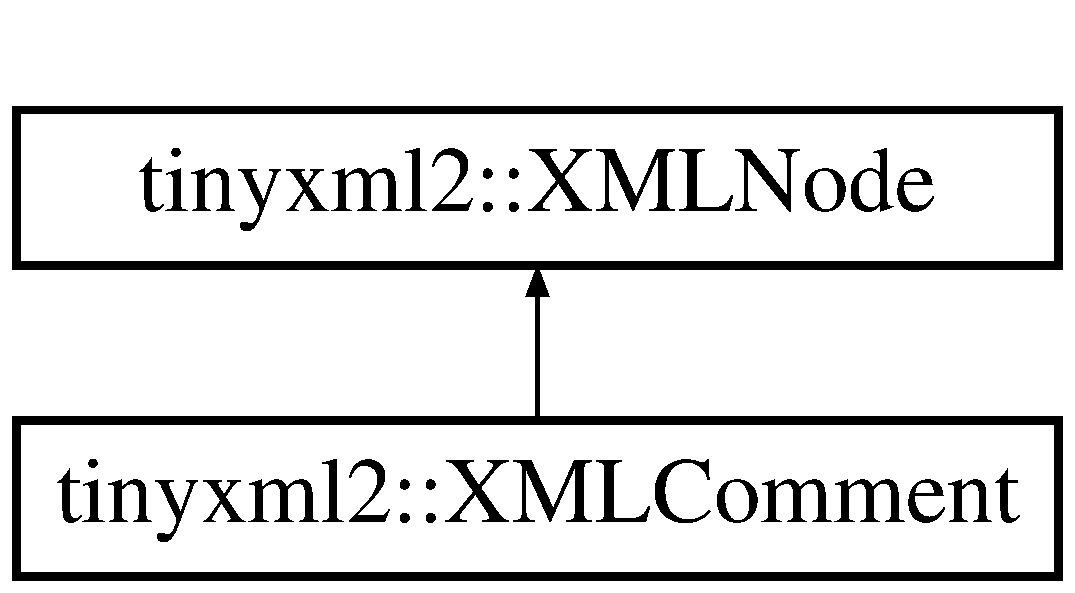
\includegraphics[height=2.000000cm]{classtinyxml2_1_1_x_m_l_comment}
\end{center}
\end{figure}
\subsection*{Public Member Functions}
\begin{DoxyCompactItemize}
\item 
\mbox{\Hypertarget{classtinyxml2_1_1_x_m_l_comment_a8093e1dc8a34fa446d9dc3fde0e6c0ee}\label{classtinyxml2_1_1_x_m_l_comment_a8093e1dc8a34fa446d9dc3fde0e6c0ee}} 
virtual \mbox{\hyperlink{classtinyxml2_1_1_x_m_l_comment}{X\+M\+L\+Comment}} $\ast$ \mbox{\hyperlink{classtinyxml2_1_1_x_m_l_comment_a8093e1dc8a34fa446d9dc3fde0e6c0ee}{To\+Comment}} ()
\begin{DoxyCompactList}\small\item\em Safely cast to a Comment, or null. \end{DoxyCompactList}\item 
\mbox{\Hypertarget{classtinyxml2_1_1_x_m_l_comment_a8e60caf06d8e88876a94b81db026b85c}\label{classtinyxml2_1_1_x_m_l_comment_a8e60caf06d8e88876a94b81db026b85c}} 
virtual const \mbox{\hyperlink{classtinyxml2_1_1_x_m_l_comment}{X\+M\+L\+Comment}} $\ast$ {\bfseries To\+Comment} () const
\item 
virtual bool \mbox{\hyperlink{classtinyxml2_1_1_x_m_l_comment_a27b37d16cea01b5329dfbbb4f9508e39}{Accept}} (\mbox{\hyperlink{classtinyxml2_1_1_x_m_l_visitor}{X\+M\+L\+Visitor}} $\ast$visitor) const
\item 
virtual \mbox{\hyperlink{classtinyxml2_1_1_x_m_l_node}{X\+M\+L\+Node}} $\ast$ \mbox{\hyperlink{classtinyxml2_1_1_x_m_l_comment_adf5b5c0319351dcc339df098d11e8fb2}{Shallow\+Clone}} (\mbox{\hyperlink{classtinyxml2_1_1_x_m_l_document}{X\+M\+L\+Document}} $\ast$document) const
\item 
virtual bool \mbox{\hyperlink{classtinyxml2_1_1_x_m_l_comment_a965d880a99d58dd915caa88dc37a9b51}{Shallow\+Equal}} (const \mbox{\hyperlink{classtinyxml2_1_1_x_m_l_node}{X\+M\+L\+Node}} $\ast$compare) const
\end{DoxyCompactItemize}
\subsection*{Protected Member Functions}
\begin{DoxyCompactItemize}
\item 
\mbox{\Hypertarget{classtinyxml2_1_1_x_m_l_comment_ae6463adc3edd93a8e5a9b2b7e99cdf91}\label{classtinyxml2_1_1_x_m_l_comment_ae6463adc3edd93a8e5a9b2b7e99cdf91}} 
{\bfseries X\+M\+L\+Comment} (\mbox{\hyperlink{classtinyxml2_1_1_x_m_l_document}{X\+M\+L\+Document}} $\ast$doc)
\item 
\mbox{\Hypertarget{classtinyxml2_1_1_x_m_l_comment_a3430281eed8d1023bafa9e633f44f509}\label{classtinyxml2_1_1_x_m_l_comment_a3430281eed8d1023bafa9e633f44f509}} 
char $\ast$ {\bfseries Parse\+Deep} (char $\ast$p, \mbox{\hyperlink{classtinyxml2_1_1_str_pair}{Str\+Pair}} $\ast$parent\+End\+Tag, int $\ast$cur\+Line\+Num\+Ptr)
\end{DoxyCompactItemize}
\subsection*{Friends}
\begin{DoxyCompactItemize}
\item 
\mbox{\Hypertarget{classtinyxml2_1_1_x_m_l_comment_a4eee3bda60c60a30e4e8cd4ea91c4c6e}\label{classtinyxml2_1_1_x_m_l_comment_a4eee3bda60c60a30e4e8cd4ea91c4c6e}} 
class {\bfseries X\+M\+L\+Document}
\end{DoxyCompactItemize}
\subsection*{Additional Inherited Members}


\subsection{Detailed Description}
An X\+ML Comment. 

\subsection{Member Function Documentation}
\mbox{\Hypertarget{classtinyxml2_1_1_x_m_l_comment_a27b37d16cea01b5329dfbbb4f9508e39}\label{classtinyxml2_1_1_x_m_l_comment_a27b37d16cea01b5329dfbbb4f9508e39}} 
\index{tinyxml2\+::\+X\+M\+L\+Comment@{tinyxml2\+::\+X\+M\+L\+Comment}!Accept@{Accept}}
\index{Accept@{Accept}!tinyxml2\+::\+X\+M\+L\+Comment@{tinyxml2\+::\+X\+M\+L\+Comment}}
\subsubsection{\texorpdfstring{Accept()}{Accept()}}
{\footnotesize\ttfamily bool tinyxml2\+::\+X\+M\+L\+Comment\+::\+Accept (\begin{DoxyParamCaption}\item[{\mbox{\hyperlink{classtinyxml2_1_1_x_m_l_visitor}{X\+M\+L\+Visitor}} $\ast$}]{visitor }\end{DoxyParamCaption}) const\hspace{0.3cm}{\ttfamily [virtual]}}

Accept a hierarchical visit of the nodes in the Tiny\+X\+M\+L-\/2 D\+OM. Every node in the X\+ML tree will be conditionally visited and the host will be called back via the \mbox{\hyperlink{classtinyxml2_1_1_x_m_l_visitor}{X\+M\+L\+Visitor}} interface.

This is essentially a S\+AX interface for Tiny\+X\+M\+L-\/2. (Note however it doesn\textquotesingle{}t re-\/parse the X\+ML for the callbacks, so the performance of Tiny\+X\+M\+L-\/2 is unchanged by using this interface versus any other.)

The interface has been based on ideas from\+:


\begin{DoxyItemize}
\item \href{http://www.saxproject.org/}{\tt http\+://www.\+saxproject.\+org/}
\item \href{http://c2.com/cgi/wiki?HierarchicalVisitorPattern}{\tt http\+://c2.\+com/cgi/wiki?\+Hierarchical\+Visitor\+Pattern}
\end{DoxyItemize}

Which are both good references for \char`\"{}visiting\char`\"{}.

An example of using \mbox{\hyperlink{classtinyxml2_1_1_x_m_l_comment_a27b37d16cea01b5329dfbbb4f9508e39}{Accept()}}\+: \begin{DoxyVerb}XMLPrinter printer;
tinyxmlDoc.Accept( &printer );
const char* xmlcstr = printer.CStr();
\end{DoxyVerb}
 

Implements \mbox{\hyperlink{classtinyxml2_1_1_x_m_l_node_a81e66df0a44c67a7af17f3b77a152785}{tinyxml2\+::\+X\+M\+L\+Node}}.

\mbox{\Hypertarget{classtinyxml2_1_1_x_m_l_comment_adf5b5c0319351dcc339df098d11e8fb2}\label{classtinyxml2_1_1_x_m_l_comment_adf5b5c0319351dcc339df098d11e8fb2}} 
\index{tinyxml2\+::\+X\+M\+L\+Comment@{tinyxml2\+::\+X\+M\+L\+Comment}!Shallow\+Clone@{Shallow\+Clone}}
\index{Shallow\+Clone@{Shallow\+Clone}!tinyxml2\+::\+X\+M\+L\+Comment@{tinyxml2\+::\+X\+M\+L\+Comment}}
\subsubsection{\texorpdfstring{Shallow\+Clone()}{ShallowClone()}}
{\footnotesize\ttfamily \mbox{\hyperlink{classtinyxml2_1_1_x_m_l_node}{X\+M\+L\+Node}} $\ast$ tinyxml2\+::\+X\+M\+L\+Comment\+::\+Shallow\+Clone (\begin{DoxyParamCaption}\item[{\mbox{\hyperlink{classtinyxml2_1_1_x_m_l_document}{X\+M\+L\+Document}} $\ast$}]{document }\end{DoxyParamCaption}) const\hspace{0.3cm}{\ttfamily [virtual]}}

Make a copy of this node, but not its children. You may pass in a Document pointer that will be the owner of the new Node. If the \textquotesingle{}document\textquotesingle{} is null, then the node returned will be allocated from the current Document. (this-\/$>$\mbox{\hyperlink{classtinyxml2_1_1_x_m_l_node_af343d1ef0b45c0020e62d784d7e67a68}{Get\+Document()}})

Note\+: if called on a \mbox{\hyperlink{classtinyxml2_1_1_x_m_l_document}{X\+M\+L\+Document}}, this will return null. 

Implements \mbox{\hyperlink{classtinyxml2_1_1_x_m_l_node_a8402cbd3129d20e9e6024bbcc0531283}{tinyxml2\+::\+X\+M\+L\+Node}}.

\mbox{\Hypertarget{classtinyxml2_1_1_x_m_l_comment_a965d880a99d58dd915caa88dc37a9b51}\label{classtinyxml2_1_1_x_m_l_comment_a965d880a99d58dd915caa88dc37a9b51}} 
\index{tinyxml2\+::\+X\+M\+L\+Comment@{tinyxml2\+::\+X\+M\+L\+Comment}!Shallow\+Equal@{Shallow\+Equal}}
\index{Shallow\+Equal@{Shallow\+Equal}!tinyxml2\+::\+X\+M\+L\+Comment@{tinyxml2\+::\+X\+M\+L\+Comment}}
\subsubsection{\texorpdfstring{Shallow\+Equal()}{ShallowEqual()}}
{\footnotesize\ttfamily bool tinyxml2\+::\+X\+M\+L\+Comment\+::\+Shallow\+Equal (\begin{DoxyParamCaption}\item[{const \mbox{\hyperlink{classtinyxml2_1_1_x_m_l_node}{X\+M\+L\+Node}} $\ast$}]{compare }\end{DoxyParamCaption}) const\hspace{0.3cm}{\ttfamily [virtual]}}

Test if 2 nodes are the same, but don\textquotesingle{}t test children. The 2 nodes do not need to be in the same Document.

Note\+: if called on a \mbox{\hyperlink{classtinyxml2_1_1_x_m_l_document}{X\+M\+L\+Document}}, this will return false. 

Implements \mbox{\hyperlink{classtinyxml2_1_1_x_m_l_node_a7ce18b751c3ea09eac292dca264f9226}{tinyxml2\+::\+X\+M\+L\+Node}}.



The documentation for this class was generated from the following files\+:\begin{DoxyCompactItemize}
\item 
Source/\+Utils/tinyxml2.\+h\item 
Source/\+Utils/tinyxml2.\+cpp\end{DoxyCompactItemize}

\hypertarget{classtinyxml2_1_1_x_m_l_const_handle}{}\section{tinyxml2\+:\+:X\+M\+L\+Const\+Handle Class Reference}
\label{classtinyxml2_1_1_x_m_l_const_handle}\index{tinyxml2\+::\+X\+M\+L\+Const\+Handle@{tinyxml2\+::\+X\+M\+L\+Const\+Handle}}


{\ttfamily \#include $<$tinyxml2.\+h$>$}

\subsection*{Public Member Functions}
\begin{DoxyCompactItemize}
\item 
\mbox{\Hypertarget{classtinyxml2_1_1_x_m_l_const_handle_a098bda71fa11d7c74ccddab59d5dd534}\label{classtinyxml2_1_1_x_m_l_const_handle_a098bda71fa11d7c74ccddab59d5dd534}} 
{\bfseries X\+M\+L\+Const\+Handle} (const \mbox{\hyperlink{classtinyxml2_1_1_x_m_l_node}{X\+M\+L\+Node}} $\ast$node)
\item 
\mbox{\Hypertarget{classtinyxml2_1_1_x_m_l_const_handle_a8420a0c4720637e0529e78c2e22f2b0b}\label{classtinyxml2_1_1_x_m_l_const_handle_a8420a0c4720637e0529e78c2e22f2b0b}} 
{\bfseries X\+M\+L\+Const\+Handle} (const \mbox{\hyperlink{classtinyxml2_1_1_x_m_l_node}{X\+M\+L\+Node}} \&node)
\item 
\mbox{\Hypertarget{classtinyxml2_1_1_x_m_l_const_handle_a639317ad315ff24f4ef0dc69312d7303}\label{classtinyxml2_1_1_x_m_l_const_handle_a639317ad315ff24f4ef0dc69312d7303}} 
{\bfseries X\+M\+L\+Const\+Handle} (const \mbox{\hyperlink{classtinyxml2_1_1_x_m_l_const_handle}{X\+M\+L\+Const\+Handle}} \&ref)
\item 
\mbox{\Hypertarget{classtinyxml2_1_1_x_m_l_const_handle_a2d74c91df1ff9aa5f9b57e3dceddbf94}\label{classtinyxml2_1_1_x_m_l_const_handle_a2d74c91df1ff9aa5f9b57e3dceddbf94}} 
\mbox{\hyperlink{classtinyxml2_1_1_x_m_l_const_handle}{X\+M\+L\+Const\+Handle}} \& {\bfseries operator=} (const \mbox{\hyperlink{classtinyxml2_1_1_x_m_l_const_handle}{X\+M\+L\+Const\+Handle}} \&ref)
\item 
\mbox{\Hypertarget{classtinyxml2_1_1_x_m_l_const_handle_aef06bd16cb308652a32b864b0a743136}\label{classtinyxml2_1_1_x_m_l_const_handle_aef06bd16cb308652a32b864b0a743136}} 
const \mbox{\hyperlink{classtinyxml2_1_1_x_m_l_const_handle}{X\+M\+L\+Const\+Handle}} {\bfseries First\+Child} () const
\item 
\mbox{\Hypertarget{classtinyxml2_1_1_x_m_l_const_handle_ac747db472ffc55c5af2e82ffec813640}\label{classtinyxml2_1_1_x_m_l_const_handle_ac747db472ffc55c5af2e82ffec813640}} 
const \mbox{\hyperlink{classtinyxml2_1_1_x_m_l_const_handle}{X\+M\+L\+Const\+Handle}} {\bfseries First\+Child\+Element} (const char $\ast$name=0) const
\item 
\mbox{\Hypertarget{classtinyxml2_1_1_x_m_l_const_handle_a908436124990f3d7b35cb7df20d31d9e}\label{classtinyxml2_1_1_x_m_l_const_handle_a908436124990f3d7b35cb7df20d31d9e}} 
const \mbox{\hyperlink{classtinyxml2_1_1_x_m_l_const_handle}{X\+M\+L\+Const\+Handle}} {\bfseries Last\+Child} () const
\item 
\mbox{\Hypertarget{classtinyxml2_1_1_x_m_l_const_handle_a9de0475ec42bd50c0e64624a250ba5b2}\label{classtinyxml2_1_1_x_m_l_const_handle_a9de0475ec42bd50c0e64624a250ba5b2}} 
const \mbox{\hyperlink{classtinyxml2_1_1_x_m_l_const_handle}{X\+M\+L\+Const\+Handle}} {\bfseries Last\+Child\+Element} (const char $\ast$name=0) const
\item 
\mbox{\Hypertarget{classtinyxml2_1_1_x_m_l_const_handle_acf68cc7930e4ac883e0c7e16ef2fbb66}\label{classtinyxml2_1_1_x_m_l_const_handle_acf68cc7930e4ac883e0c7e16ef2fbb66}} 
const \mbox{\hyperlink{classtinyxml2_1_1_x_m_l_const_handle}{X\+M\+L\+Const\+Handle}} {\bfseries Previous\+Sibling} () const
\item 
\mbox{\Hypertarget{classtinyxml2_1_1_x_m_l_const_handle_aef99308659f2617299ac29980769a91e}\label{classtinyxml2_1_1_x_m_l_const_handle_aef99308659f2617299ac29980769a91e}} 
const \mbox{\hyperlink{classtinyxml2_1_1_x_m_l_const_handle}{X\+M\+L\+Const\+Handle}} {\bfseries Previous\+Sibling\+Element} (const char $\ast$name=0) const
\item 
\mbox{\Hypertarget{classtinyxml2_1_1_x_m_l_const_handle_aec3710e455f41014026ef17fbbb0efb3}\label{classtinyxml2_1_1_x_m_l_const_handle_aec3710e455f41014026ef17fbbb0efb3}} 
const \mbox{\hyperlink{classtinyxml2_1_1_x_m_l_const_handle}{X\+M\+L\+Const\+Handle}} {\bfseries Next\+Sibling} () const
\item 
\mbox{\Hypertarget{classtinyxml2_1_1_x_m_l_const_handle_a3c9e6b48b02d3d5232e1e8780753d8a5}\label{classtinyxml2_1_1_x_m_l_const_handle_a3c9e6b48b02d3d5232e1e8780753d8a5}} 
const \mbox{\hyperlink{classtinyxml2_1_1_x_m_l_const_handle}{X\+M\+L\+Const\+Handle}} {\bfseries Next\+Sibling\+Element} (const char $\ast$name=0) const
\item 
\mbox{\Hypertarget{classtinyxml2_1_1_x_m_l_const_handle_a61812760cb08bc1b050e65b73a08457b}\label{classtinyxml2_1_1_x_m_l_const_handle_a61812760cb08bc1b050e65b73a08457b}} 
const \mbox{\hyperlink{classtinyxml2_1_1_x_m_l_node}{X\+M\+L\+Node}} $\ast$ {\bfseries To\+Node} () const
\item 
\mbox{\Hypertarget{classtinyxml2_1_1_x_m_l_const_handle_a4dba53c6e201d412e915620feaaa56f3}\label{classtinyxml2_1_1_x_m_l_const_handle_a4dba53c6e201d412e915620feaaa56f3}} 
const \mbox{\hyperlink{classtinyxml2_1_1_x_m_l_element}{X\+M\+L\+Element}} $\ast$ {\bfseries To\+Element} () const
\item 
\mbox{\Hypertarget{classtinyxml2_1_1_x_m_l_const_handle_a80e24d90d476005aa35602a665358e2d}\label{classtinyxml2_1_1_x_m_l_const_handle_a80e24d90d476005aa35602a665358e2d}} 
const \mbox{\hyperlink{classtinyxml2_1_1_x_m_l_text}{X\+M\+L\+Text}} $\ast$ {\bfseries To\+Text} () const
\item 
\mbox{\Hypertarget{classtinyxml2_1_1_x_m_l_const_handle_a4395e5feaba7b456a81ca274880ea3d3}\label{classtinyxml2_1_1_x_m_l_const_handle_a4395e5feaba7b456a81ca274880ea3d3}} 
const \mbox{\hyperlink{classtinyxml2_1_1_x_m_l_unknown}{X\+M\+L\+Unknown}} $\ast$ {\bfseries To\+Unknown} () const
\item 
\mbox{\Hypertarget{classtinyxml2_1_1_x_m_l_const_handle_a55e306d105fa80d626041e4d3b77b716}\label{classtinyxml2_1_1_x_m_l_const_handle_a55e306d105fa80d626041e4d3b77b716}} 
const \mbox{\hyperlink{classtinyxml2_1_1_x_m_l_declaration}{X\+M\+L\+Declaration}} $\ast$ {\bfseries To\+Declaration} () const
\end{DoxyCompactItemize}


\subsection{Detailed Description}
A variant of the \mbox{\hyperlink{classtinyxml2_1_1_x_m_l_handle}{X\+M\+L\+Handle}} class for working with const X\+M\+L\+Nodes and Documents. It is the same in all regards, except for the \textquotesingle{}const\textquotesingle{} qualifiers. See \mbox{\hyperlink{classtinyxml2_1_1_x_m_l_handle}{X\+M\+L\+Handle}} for A\+PI. 

The documentation for this class was generated from the following file\+:\begin{DoxyCompactItemize}
\item 
Source/\+Utils/tinyxml2.\+h\end{DoxyCompactItemize}

\hypertarget{classtinyxml2_1_1_x_m_l_declaration}{}\section{tinyxml2\+:\+:X\+M\+L\+Declaration Class Reference}
\label{classtinyxml2_1_1_x_m_l_declaration}\index{tinyxml2\+::\+X\+M\+L\+Declaration@{tinyxml2\+::\+X\+M\+L\+Declaration}}


{\ttfamily \#include $<$tinyxml2.\+h$>$}

Inheritance diagram for tinyxml2\+:\+:X\+M\+L\+Declaration\+:\begin{figure}[H]
\begin{center}
\leavevmode
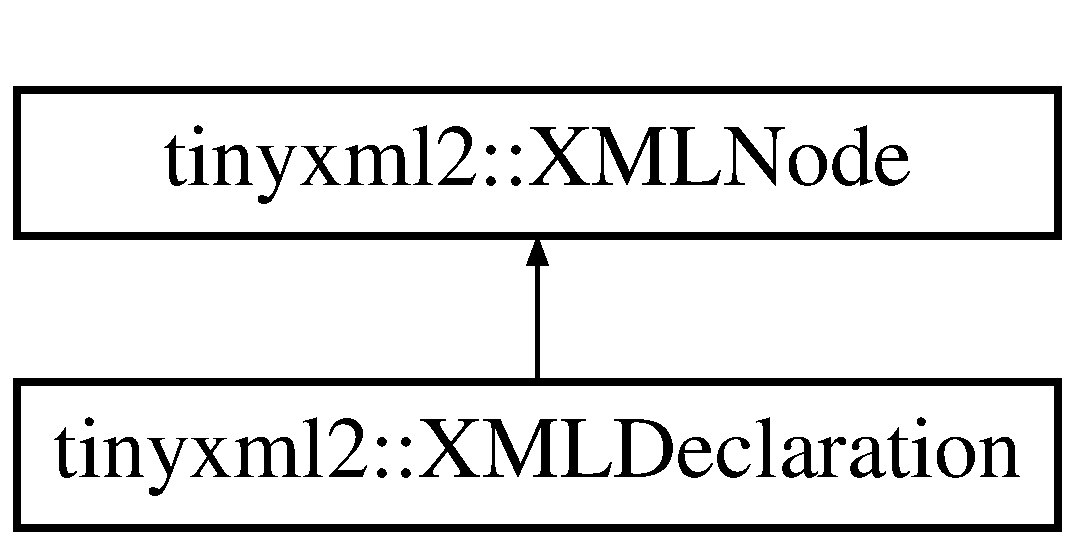
\includegraphics[height=2.000000cm]{classtinyxml2_1_1_x_m_l_declaration}
\end{center}
\end{figure}
\subsection*{Public Member Functions}
\begin{DoxyCompactItemize}
\item 
\mbox{\Hypertarget{classtinyxml2_1_1_x_m_l_declaration_a159d8ac45865215e88059ea1e5b52fc5}\label{classtinyxml2_1_1_x_m_l_declaration_a159d8ac45865215e88059ea1e5b52fc5}} 
virtual \mbox{\hyperlink{classtinyxml2_1_1_x_m_l_declaration}{X\+M\+L\+Declaration}} $\ast$ \mbox{\hyperlink{classtinyxml2_1_1_x_m_l_declaration_a159d8ac45865215e88059ea1e5b52fc5}{To\+Declaration}} ()
\begin{DoxyCompactList}\small\item\em Safely cast to a Declaration, or null. \end{DoxyCompactList}\item 
\mbox{\Hypertarget{classtinyxml2_1_1_x_m_l_declaration_aa20c3315b18c3b88830dccf5c493259b}\label{classtinyxml2_1_1_x_m_l_declaration_aa20c3315b18c3b88830dccf5c493259b}} 
virtual const \mbox{\hyperlink{classtinyxml2_1_1_x_m_l_declaration}{X\+M\+L\+Declaration}} $\ast$ {\bfseries To\+Declaration} () const
\item 
virtual bool \mbox{\hyperlink{classtinyxml2_1_1_x_m_l_declaration_acf47629d9fc08ed6f1c164a97bcf794b}{Accept}} (\mbox{\hyperlink{classtinyxml2_1_1_x_m_l_visitor}{X\+M\+L\+Visitor}} $\ast$visitor) const
\item 
virtual \mbox{\hyperlink{classtinyxml2_1_1_x_m_l_node}{X\+M\+L\+Node}} $\ast$ \mbox{\hyperlink{classtinyxml2_1_1_x_m_l_declaration_ad9d60e6d2df75c13eb6bf7319985b747}{Shallow\+Clone}} (\mbox{\hyperlink{classtinyxml2_1_1_x_m_l_document}{X\+M\+L\+Document}} $\ast$document) const
\item 
virtual bool \mbox{\hyperlink{classtinyxml2_1_1_x_m_l_declaration_ae8b4d3a399857029f36c322b0801b69c}{Shallow\+Equal}} (const \mbox{\hyperlink{classtinyxml2_1_1_x_m_l_node}{X\+M\+L\+Node}} $\ast$compare) const
\end{DoxyCompactItemize}
\subsection*{Protected Member Functions}
\begin{DoxyCompactItemize}
\item 
\mbox{\Hypertarget{classtinyxml2_1_1_x_m_l_declaration_aef9586f2ce5df5feba74dde49a242b06}\label{classtinyxml2_1_1_x_m_l_declaration_aef9586f2ce5df5feba74dde49a242b06}} 
{\bfseries X\+M\+L\+Declaration} (\mbox{\hyperlink{classtinyxml2_1_1_x_m_l_document}{X\+M\+L\+Document}} $\ast$doc)
\item 
\mbox{\Hypertarget{classtinyxml2_1_1_x_m_l_declaration_a42a2a36f4d78dc745063b79c16538b9b}\label{classtinyxml2_1_1_x_m_l_declaration_a42a2a36f4d78dc745063b79c16538b9b}} 
char $\ast$ {\bfseries Parse\+Deep} (char $\ast$p, \mbox{\hyperlink{classtinyxml2_1_1_str_pair}{Str\+Pair}} $\ast$parent\+End\+Tag, int $\ast$cur\+Line\+Num\+Ptr)
\end{DoxyCompactItemize}
\subsection*{Friends}
\begin{DoxyCompactItemize}
\item 
\mbox{\Hypertarget{classtinyxml2_1_1_x_m_l_declaration_a4eee3bda60c60a30e4e8cd4ea91c4c6e}\label{classtinyxml2_1_1_x_m_l_declaration_a4eee3bda60c60a30e4e8cd4ea91c4c6e}} 
class {\bfseries X\+M\+L\+Document}
\end{DoxyCompactItemize}
\subsection*{Additional Inherited Members}


\subsection{Detailed Description}
In correct X\+ML the declaration is the first entry in the file. \begin{DoxyVerb}    <?xml version="1.0" standalone="yes"?>
\end{DoxyVerb}


Tiny\+X\+M\+L-\/2 will happily read or write files without a declaration, however.

The text of the declaration isn\textquotesingle{}t interpreted. It is parsed and written as a string. 

\subsection{Member Function Documentation}
\mbox{\Hypertarget{classtinyxml2_1_1_x_m_l_declaration_acf47629d9fc08ed6f1c164a97bcf794b}\label{classtinyxml2_1_1_x_m_l_declaration_acf47629d9fc08ed6f1c164a97bcf794b}} 
\index{tinyxml2\+::\+X\+M\+L\+Declaration@{tinyxml2\+::\+X\+M\+L\+Declaration}!Accept@{Accept}}
\index{Accept@{Accept}!tinyxml2\+::\+X\+M\+L\+Declaration@{tinyxml2\+::\+X\+M\+L\+Declaration}}
\subsubsection{\texorpdfstring{Accept()}{Accept()}}
{\footnotesize\ttfamily bool tinyxml2\+::\+X\+M\+L\+Declaration\+::\+Accept (\begin{DoxyParamCaption}\item[{\mbox{\hyperlink{classtinyxml2_1_1_x_m_l_visitor}{X\+M\+L\+Visitor}} $\ast$}]{visitor }\end{DoxyParamCaption}) const\hspace{0.3cm}{\ttfamily [virtual]}}

Accept a hierarchical visit of the nodes in the Tiny\+X\+M\+L-\/2 D\+OM. Every node in the X\+ML tree will be conditionally visited and the host will be called back via the \mbox{\hyperlink{classtinyxml2_1_1_x_m_l_visitor}{X\+M\+L\+Visitor}} interface.

This is essentially a S\+AX interface for Tiny\+X\+M\+L-\/2. (Note however it doesn\textquotesingle{}t re-\/parse the X\+ML for the callbacks, so the performance of Tiny\+X\+M\+L-\/2 is unchanged by using this interface versus any other.)

The interface has been based on ideas from\+:


\begin{DoxyItemize}
\item \href{http://www.saxproject.org/}{\tt http\+://www.\+saxproject.\+org/}
\item \href{http://c2.com/cgi/wiki?HierarchicalVisitorPattern}{\tt http\+://c2.\+com/cgi/wiki?\+Hierarchical\+Visitor\+Pattern}
\end{DoxyItemize}

Which are both good references for \char`\"{}visiting\char`\"{}.

An example of using \mbox{\hyperlink{classtinyxml2_1_1_x_m_l_declaration_acf47629d9fc08ed6f1c164a97bcf794b}{Accept()}}\+: \begin{DoxyVerb}XMLPrinter printer;
tinyxmlDoc.Accept( &printer );
const char* xmlcstr = printer.CStr();
\end{DoxyVerb}
 

Implements \mbox{\hyperlink{classtinyxml2_1_1_x_m_l_node_a81e66df0a44c67a7af17f3b77a152785}{tinyxml2\+::\+X\+M\+L\+Node}}.

\mbox{\Hypertarget{classtinyxml2_1_1_x_m_l_declaration_ad9d60e6d2df75c13eb6bf7319985b747}\label{classtinyxml2_1_1_x_m_l_declaration_ad9d60e6d2df75c13eb6bf7319985b747}} 
\index{tinyxml2\+::\+X\+M\+L\+Declaration@{tinyxml2\+::\+X\+M\+L\+Declaration}!Shallow\+Clone@{Shallow\+Clone}}
\index{Shallow\+Clone@{Shallow\+Clone}!tinyxml2\+::\+X\+M\+L\+Declaration@{tinyxml2\+::\+X\+M\+L\+Declaration}}
\subsubsection{\texorpdfstring{Shallow\+Clone()}{ShallowClone()}}
{\footnotesize\ttfamily \mbox{\hyperlink{classtinyxml2_1_1_x_m_l_node}{X\+M\+L\+Node}} $\ast$ tinyxml2\+::\+X\+M\+L\+Declaration\+::\+Shallow\+Clone (\begin{DoxyParamCaption}\item[{\mbox{\hyperlink{classtinyxml2_1_1_x_m_l_document}{X\+M\+L\+Document}} $\ast$}]{document }\end{DoxyParamCaption}) const\hspace{0.3cm}{\ttfamily [virtual]}}

Make a copy of this node, but not its children. You may pass in a Document pointer that will be the owner of the new Node. If the \textquotesingle{}document\textquotesingle{} is null, then the node returned will be allocated from the current Document. (this-\/$>$\mbox{\hyperlink{classtinyxml2_1_1_x_m_l_node_af343d1ef0b45c0020e62d784d7e67a68}{Get\+Document()}})

Note\+: if called on a \mbox{\hyperlink{classtinyxml2_1_1_x_m_l_document}{X\+M\+L\+Document}}, this will return null. 

Implements \mbox{\hyperlink{classtinyxml2_1_1_x_m_l_node_a8402cbd3129d20e9e6024bbcc0531283}{tinyxml2\+::\+X\+M\+L\+Node}}.

\mbox{\Hypertarget{classtinyxml2_1_1_x_m_l_declaration_ae8b4d3a399857029f36c322b0801b69c}\label{classtinyxml2_1_1_x_m_l_declaration_ae8b4d3a399857029f36c322b0801b69c}} 
\index{tinyxml2\+::\+X\+M\+L\+Declaration@{tinyxml2\+::\+X\+M\+L\+Declaration}!Shallow\+Equal@{Shallow\+Equal}}
\index{Shallow\+Equal@{Shallow\+Equal}!tinyxml2\+::\+X\+M\+L\+Declaration@{tinyxml2\+::\+X\+M\+L\+Declaration}}
\subsubsection{\texorpdfstring{Shallow\+Equal()}{ShallowEqual()}}
{\footnotesize\ttfamily bool tinyxml2\+::\+X\+M\+L\+Declaration\+::\+Shallow\+Equal (\begin{DoxyParamCaption}\item[{const \mbox{\hyperlink{classtinyxml2_1_1_x_m_l_node}{X\+M\+L\+Node}} $\ast$}]{compare }\end{DoxyParamCaption}) const\hspace{0.3cm}{\ttfamily [virtual]}}

Test if 2 nodes are the same, but don\textquotesingle{}t test children. The 2 nodes do not need to be in the same Document.

Note\+: if called on a \mbox{\hyperlink{classtinyxml2_1_1_x_m_l_document}{X\+M\+L\+Document}}, this will return false. 

Implements \mbox{\hyperlink{classtinyxml2_1_1_x_m_l_node_a7ce18b751c3ea09eac292dca264f9226}{tinyxml2\+::\+X\+M\+L\+Node}}.



The documentation for this class was generated from the following files\+:\begin{DoxyCompactItemize}
\item 
Source/\+Utils/tinyxml2.\+h\item 
Source/\+Utils/tinyxml2.\+cpp\end{DoxyCompactItemize}

\hypertarget{classtinyxml2_1_1_x_m_l_document}{}\section{tinyxml2\+:\+:X\+M\+L\+Document Class Reference}
\label{classtinyxml2_1_1_x_m_l_document}\index{tinyxml2\+::\+X\+M\+L\+Document@{tinyxml2\+::\+X\+M\+L\+Document}}


{\ttfamily \#include $<$tinyxml2.\+h$>$}

Inheritance diagram for tinyxml2\+:\+:X\+M\+L\+Document\+:\begin{figure}[H]
\begin{center}
\leavevmode
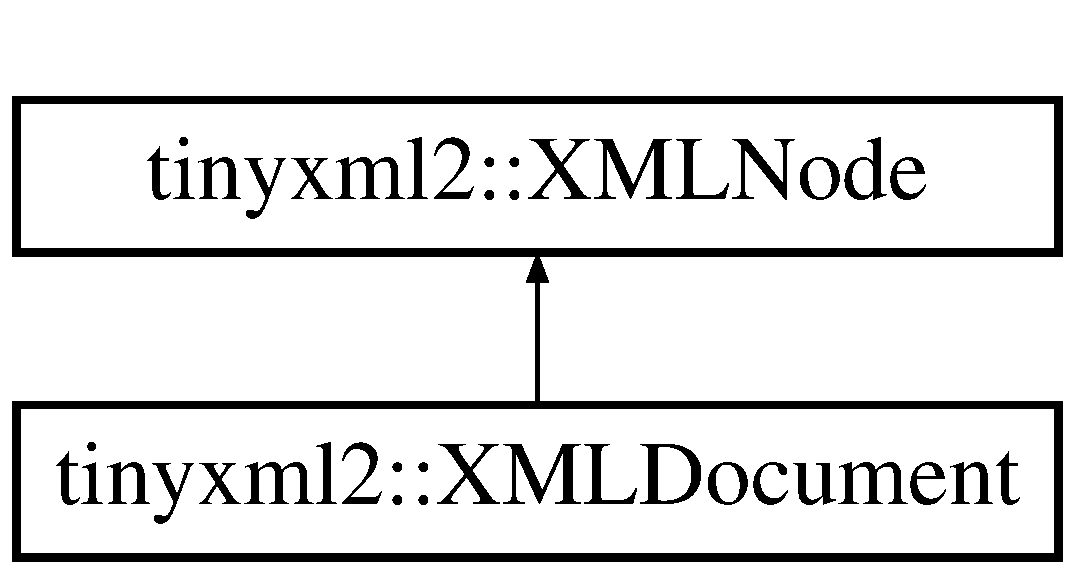
\includegraphics[height=2.000000cm]{classtinyxml2_1_1_x_m_l_document}
\end{center}
\end{figure}
\subsection*{Public Member Functions}
\begin{DoxyCompactItemize}
\item 
\mbox{\Hypertarget{classtinyxml2_1_1_x_m_l_document_a57ddf17b6e054dda10af98991b1b8f70}\label{classtinyxml2_1_1_x_m_l_document_a57ddf17b6e054dda10af98991b1b8f70}} 
\mbox{\hyperlink{classtinyxml2_1_1_x_m_l_document_a57ddf17b6e054dda10af98991b1b8f70}{X\+M\+L\+Document}} (bool process\+Entities=true, Whitespace whitespace\+Mode=P\+R\+E\+S\+E\+R\+V\+E\+\_\+\+W\+H\+I\+T\+E\+S\+P\+A\+CE)
\begin{DoxyCompactList}\small\item\em constructor \end{DoxyCompactList}\item 
\mbox{\Hypertarget{classtinyxml2_1_1_x_m_l_document_a3e185f880882bd978367bb55937735ec}\label{classtinyxml2_1_1_x_m_l_document_a3e185f880882bd978367bb55937735ec}} 
virtual \mbox{\hyperlink{classtinyxml2_1_1_x_m_l_document}{X\+M\+L\+Document}} $\ast$ \mbox{\hyperlink{classtinyxml2_1_1_x_m_l_document_a3e185f880882bd978367bb55937735ec}{To\+Document}} ()
\begin{DoxyCompactList}\small\item\em Safely cast to a Document, or null. \end{DoxyCompactList}\item 
\mbox{\Hypertarget{classtinyxml2_1_1_x_m_l_document_a747ab173887d969fe313b4617f968e99}\label{classtinyxml2_1_1_x_m_l_document_a747ab173887d969fe313b4617f968e99}} 
virtual const \mbox{\hyperlink{classtinyxml2_1_1_x_m_l_document}{X\+M\+L\+Document}} $\ast$ {\bfseries To\+Document} () const
\item 
X\+M\+L\+Error \mbox{\hyperlink{classtinyxml2_1_1_x_m_l_document_a1819bd34f540a7304c105a6232d25a1f}{Parse}} (const char $\ast$xml, size\+\_\+t n\+Bytes=(size\+\_\+t)(-\/1))
\item 
X\+M\+L\+Error \mbox{\hyperlink{classtinyxml2_1_1_x_m_l_document_a2ebd4647a8af5fc6831b294ac26a150a}{Load\+File}} (const char $\ast$filename)
\item 
X\+M\+L\+Error \mbox{\hyperlink{classtinyxml2_1_1_x_m_l_document_a5f1d330fad44c52f3d265338dd2a6dc2}{Load\+File}} (F\+I\+LE $\ast$)
\item 
X\+M\+L\+Error \mbox{\hyperlink{classtinyxml2_1_1_x_m_l_document_a73ac416b4a2aa0952e841220eb3da18f}{Save\+File}} (const char $\ast$filename, bool compact=false)
\item 
X\+M\+L\+Error \mbox{\hyperlink{classtinyxml2_1_1_x_m_l_document_a8b95779479a0035acc67b3a61dfe1b74}{Save\+File}} (F\+I\+LE $\ast$fp, bool compact=false)
\item 
\mbox{\Hypertarget{classtinyxml2_1_1_x_m_l_document_a53e6c035b1b539563fef8c817fb30469}\label{classtinyxml2_1_1_x_m_l_document_a53e6c035b1b539563fef8c817fb30469}} 
bool {\bfseries Process\+Entities} () const
\item 
\mbox{\Hypertarget{classtinyxml2_1_1_x_m_l_document_a810ce508e6e0365497c2a9deb83c9ca7}\label{classtinyxml2_1_1_x_m_l_document_a810ce508e6e0365497c2a9deb83c9ca7}} 
Whitespace {\bfseries Whitespace\+Mode} () const
\item 
bool \mbox{\hyperlink{classtinyxml2_1_1_x_m_l_document_a33fc5d159db873a179fa26338adb05bd}{Has\+B\+OM}} () const
\item 
void \mbox{\hyperlink{classtinyxml2_1_1_x_m_l_document_a14419b698f7c4b140df4e80f3f0c93b0}{Set\+B\+OM}} (bool use\+B\+OM)
\item 
\mbox{\hyperlink{classtinyxml2_1_1_x_m_l_element}{X\+M\+L\+Element}} $\ast$ \mbox{\hyperlink{classtinyxml2_1_1_x_m_l_document_ad2b70320d3c2a071c2f36928edff3e1c}{Root\+Element}} ()
\item 
\mbox{\Hypertarget{classtinyxml2_1_1_x_m_l_document_a2be8ef9d6346bdef34311f91529afae4}\label{classtinyxml2_1_1_x_m_l_document_a2be8ef9d6346bdef34311f91529afae4}} 
const \mbox{\hyperlink{classtinyxml2_1_1_x_m_l_element}{X\+M\+L\+Element}} $\ast$ {\bfseries Root\+Element} () const
\item 
void \mbox{\hyperlink{classtinyxml2_1_1_x_m_l_document_a867cf5fa3e3ff6ae4847a8b7ee8ec083}{Print}} (\mbox{\hyperlink{classtinyxml2_1_1_x_m_l_printer}{X\+M\+L\+Printer}} $\ast$streamer=0) const
\item 
virtual bool \mbox{\hyperlink{classtinyxml2_1_1_x_m_l_document_ab7be651917a35ab1ff0e4e6d4e565cdf}{Accept}} (\mbox{\hyperlink{classtinyxml2_1_1_x_m_l_visitor}{X\+M\+L\+Visitor}} $\ast$visitor) const
\item 
\mbox{\hyperlink{classtinyxml2_1_1_x_m_l_element}{X\+M\+L\+Element}} $\ast$ \mbox{\hyperlink{classtinyxml2_1_1_x_m_l_document_a3c335a700a43d7c363a393142a23f234}{New\+Element}} (const char $\ast$name)
\item 
\mbox{\hyperlink{classtinyxml2_1_1_x_m_l_comment}{X\+M\+L\+Comment}} $\ast$ \mbox{\hyperlink{classtinyxml2_1_1_x_m_l_document_a386df0befd06aadb5e0cd21381aa955a}{New\+Comment}} (const char $\ast$comment)
\item 
\mbox{\hyperlink{classtinyxml2_1_1_x_m_l_text}{X\+M\+L\+Text}} $\ast$ \mbox{\hyperlink{classtinyxml2_1_1_x_m_l_document_acece5de77a0819f2341b08c1e1ed9987}{New\+Text}} (const char $\ast$text)
\item 
\mbox{\hyperlink{classtinyxml2_1_1_x_m_l_declaration}{X\+M\+L\+Declaration}} $\ast$ \mbox{\hyperlink{classtinyxml2_1_1_x_m_l_document_ae519030c0262fa2daff8993681990e16}{New\+Declaration}} (const char $\ast$text=0)
\item 
\mbox{\hyperlink{classtinyxml2_1_1_x_m_l_unknown}{X\+M\+L\+Unknown}} $\ast$ \mbox{\hyperlink{classtinyxml2_1_1_x_m_l_document_a4954f502c5fd7f49de54c3c0c99bb73d}{New\+Unknown}} (const char $\ast$text)
\item 
void \mbox{\hyperlink{classtinyxml2_1_1_x_m_l_document_ac1d6e2c7fcc1a660624ac4f68e96380d}{Delete\+Node}} (\mbox{\hyperlink{classtinyxml2_1_1_x_m_l_node}{X\+M\+L\+Node}} $\ast$node)
\item 
\mbox{\Hypertarget{classtinyxml2_1_1_x_m_l_document_a4085d9c52f1d93214311459d6d1fcf17}\label{classtinyxml2_1_1_x_m_l_document_a4085d9c52f1d93214311459d6d1fcf17}} 
void {\bfseries Clear\+Error} ()
\item 
\mbox{\Hypertarget{classtinyxml2_1_1_x_m_l_document_a34e6318e182e40e3cc4f4ba5d59ed9ed}\label{classtinyxml2_1_1_x_m_l_document_a34e6318e182e40e3cc4f4ba5d59ed9ed}} 
bool \mbox{\hyperlink{classtinyxml2_1_1_x_m_l_document_a34e6318e182e40e3cc4f4ba5d59ed9ed}{Error}} () const
\begin{DoxyCompactList}\small\item\em Return true if there was an error parsing the document. \end{DoxyCompactList}\item 
\mbox{\Hypertarget{classtinyxml2_1_1_x_m_l_document_afa3ed33b3107f920ec2b301f805ac17d}\label{classtinyxml2_1_1_x_m_l_document_afa3ed33b3107f920ec2b301f805ac17d}} 
X\+M\+L\+Error \mbox{\hyperlink{classtinyxml2_1_1_x_m_l_document_afa3ed33b3107f920ec2b301f805ac17d}{Error\+ID}} () const
\begin{DoxyCompactList}\small\item\em Return the error\+ID. \end{DoxyCompactList}\item 
\mbox{\Hypertarget{classtinyxml2_1_1_x_m_l_document_a1a5f2b63427caffd4cde15781d9d11f9}\label{classtinyxml2_1_1_x_m_l_document_a1a5f2b63427caffd4cde15781d9d11f9}} 
const char $\ast$ {\bfseries Error\+Name} () const
\item 
const char $\ast$ \mbox{\hyperlink{classtinyxml2_1_1_x_m_l_document_ae97fff2402a0d01e0509c430b37996b3}{Error\+Str}} () const
\item 
\mbox{\Hypertarget{classtinyxml2_1_1_x_m_l_document_a1d033945b42e125d933d6231e4571552}\label{classtinyxml2_1_1_x_m_l_document_a1d033945b42e125d933d6231e4571552}} 
void \mbox{\hyperlink{classtinyxml2_1_1_x_m_l_document_a1d033945b42e125d933d6231e4571552}{Print\+Error}} () const
\begin{DoxyCompactList}\small\item\em A (trivial) utility function that prints the \mbox{\hyperlink{classtinyxml2_1_1_x_m_l_document_ae97fff2402a0d01e0509c430b37996b3}{Error\+Str()}} to stdout. \end{DoxyCompactList}\item 
\mbox{\Hypertarget{classtinyxml2_1_1_x_m_l_document_a57400f816dbe7799ece33615ead9ab76}\label{classtinyxml2_1_1_x_m_l_document_a57400f816dbe7799ece33615ead9ab76}} 
int \mbox{\hyperlink{classtinyxml2_1_1_x_m_l_document_a57400f816dbe7799ece33615ead9ab76}{Error\+Line\+Num}} () const
\begin{DoxyCompactList}\small\item\em Return the line where the error occured, or zero if unknown. \end{DoxyCompactList}\item 
\mbox{\Hypertarget{classtinyxml2_1_1_x_m_l_document_a65656b0b2cbc822708eb351504178aaf}\label{classtinyxml2_1_1_x_m_l_document_a65656b0b2cbc822708eb351504178aaf}} 
void \mbox{\hyperlink{classtinyxml2_1_1_x_m_l_document_a65656b0b2cbc822708eb351504178aaf}{Clear}} ()
\begin{DoxyCompactList}\small\item\em Clear the document, resetting it to the initial state. \end{DoxyCompactList}\item 
void \mbox{\hyperlink{classtinyxml2_1_1_x_m_l_document_af592ffc91514e25a39664521ac83db45}{Deep\+Copy}} (\mbox{\hyperlink{classtinyxml2_1_1_x_m_l_document}{X\+M\+L\+Document}} $\ast$target) const
\item 
\mbox{\Hypertarget{classtinyxml2_1_1_x_m_l_document_a25827d1bec509ad566a107e5853ed040}\label{classtinyxml2_1_1_x_m_l_document_a25827d1bec509ad566a107e5853ed040}} 
char $\ast$ {\bfseries Identify} (char $\ast$p, \mbox{\hyperlink{classtinyxml2_1_1_x_m_l_node}{X\+M\+L\+Node}} $\ast$$\ast$node)
\item 
\mbox{\Hypertarget{classtinyxml2_1_1_x_m_l_document_a95d28ecb4760a994556b0a51690b21be}\label{classtinyxml2_1_1_x_m_l_document_a95d28ecb4760a994556b0a51690b21be}} 
void {\bfseries Mark\+In\+Use} (\mbox{\hyperlink{classtinyxml2_1_1_x_m_l_node}{X\+M\+L\+Node}} $\ast$)
\item 
virtual \mbox{\hyperlink{classtinyxml2_1_1_x_m_l_node}{X\+M\+L\+Node}} $\ast$ \mbox{\hyperlink{classtinyxml2_1_1_x_m_l_document_aa37cc1709d7e1e988bc17dcfb24a69b8}{Shallow\+Clone}} (\mbox{\hyperlink{classtinyxml2_1_1_x_m_l_document}{X\+M\+L\+Document}} $\ast$) const
\item 
virtual bool \mbox{\hyperlink{classtinyxml2_1_1_x_m_l_document_a6fe5ef18699091844fcf64b56ffa5bf9}{Shallow\+Equal}} (const \mbox{\hyperlink{classtinyxml2_1_1_x_m_l_node}{X\+M\+L\+Node}} $\ast$) const
\end{DoxyCompactItemize}
\subsection*{Static Public Member Functions}
\begin{DoxyCompactItemize}
\item 
\mbox{\Hypertarget{classtinyxml2_1_1_x_m_l_document_a639f7c295c38dc5a4aafeb2fff93da03}\label{classtinyxml2_1_1_x_m_l_document_a639f7c295c38dc5a4aafeb2fff93da03}} 
static const char $\ast$ {\bfseries Error\+I\+D\+To\+Name} (X\+M\+L\+Error error\+ID)
\end{DoxyCompactItemize}
\subsection*{Friends}
\begin{DoxyCompactItemize}
\item 
\mbox{\Hypertarget{classtinyxml2_1_1_x_m_l_document_ac2fba9b6e452829dd892f7392c24e0eb}\label{classtinyxml2_1_1_x_m_l_document_ac2fba9b6e452829dd892f7392c24e0eb}} 
class {\bfseries X\+M\+L\+Element}
\item 
\mbox{\Hypertarget{classtinyxml2_1_1_x_m_l_document_a8233f9dc4d61d90e93be2a3647c6d957}\label{classtinyxml2_1_1_x_m_l_document_a8233f9dc4d61d90e93be2a3647c6d957}} 
class {\bfseries X\+M\+L\+Node}
\item 
\mbox{\Hypertarget{classtinyxml2_1_1_x_m_l_document_ae50b59416e98bbe7e4bc87df40092109}\label{classtinyxml2_1_1_x_m_l_document_ae50b59416e98bbe7e4bc87df40092109}} 
class {\bfseries X\+M\+L\+Text}
\item 
\mbox{\Hypertarget{classtinyxml2_1_1_x_m_l_document_acee9e261162d4236fb2c30312c54cd4c}\label{classtinyxml2_1_1_x_m_l_document_acee9e261162d4236fb2c30312c54cd4c}} 
class {\bfseries X\+M\+L\+Comment}
\item 
\mbox{\Hypertarget{classtinyxml2_1_1_x_m_l_document_a93d2c2c2db3973083b7d6e7f6f358160}\label{classtinyxml2_1_1_x_m_l_document_a93d2c2c2db3973083b7d6e7f6f358160}} 
class {\bfseries X\+M\+L\+Declaration}
\item 
\mbox{\Hypertarget{classtinyxml2_1_1_x_m_l_document_a6946948274f7a02f5e69b5dbeaea9b35}\label{classtinyxml2_1_1_x_m_l_document_a6946948274f7a02f5e69b5dbeaea9b35}} 
class {\bfseries X\+M\+L\+Unknown}
\end{DoxyCompactItemize}
\subsection*{Additional Inherited Members}


\subsection{Detailed Description}
A Document binds together all the functionality. It can be saved, loaded, and printed to the screen. All Nodes are connected and allocated to a Document. If the Document is deleted, all its Nodes are also deleted. 

\subsection{Member Function Documentation}
\mbox{\Hypertarget{classtinyxml2_1_1_x_m_l_document_ab7be651917a35ab1ff0e4e6d4e565cdf}\label{classtinyxml2_1_1_x_m_l_document_ab7be651917a35ab1ff0e4e6d4e565cdf}} 
\index{tinyxml2\+::\+X\+M\+L\+Document@{tinyxml2\+::\+X\+M\+L\+Document}!Accept@{Accept}}
\index{Accept@{Accept}!tinyxml2\+::\+X\+M\+L\+Document@{tinyxml2\+::\+X\+M\+L\+Document}}
\subsubsection{\texorpdfstring{Accept()}{Accept()}}
{\footnotesize\ttfamily bool tinyxml2\+::\+X\+M\+L\+Document\+::\+Accept (\begin{DoxyParamCaption}\item[{\mbox{\hyperlink{classtinyxml2_1_1_x_m_l_visitor}{X\+M\+L\+Visitor}} $\ast$}]{visitor }\end{DoxyParamCaption}) const\hspace{0.3cm}{\ttfamily [virtual]}}

Accept a hierarchical visit of the nodes in the Tiny\+X\+M\+L-\/2 D\+OM. Every node in the X\+ML tree will be conditionally visited and the host will be called back via the \mbox{\hyperlink{classtinyxml2_1_1_x_m_l_visitor}{X\+M\+L\+Visitor}} interface.

This is essentially a S\+AX interface for Tiny\+X\+M\+L-\/2. (Note however it doesn\textquotesingle{}t re-\/parse the X\+ML for the callbacks, so the performance of Tiny\+X\+M\+L-\/2 is unchanged by using this interface versus any other.)

The interface has been based on ideas from\+:


\begin{DoxyItemize}
\item \href{http://www.saxproject.org/}{\tt http\+://www.\+saxproject.\+org/}
\item \href{http://c2.com/cgi/wiki?HierarchicalVisitorPattern}{\tt http\+://c2.\+com/cgi/wiki?\+Hierarchical\+Visitor\+Pattern}
\end{DoxyItemize}

Which are both good references for \char`\"{}visiting\char`\"{}.

An example of using \mbox{\hyperlink{classtinyxml2_1_1_x_m_l_document_ab7be651917a35ab1ff0e4e6d4e565cdf}{Accept()}}\+: \begin{DoxyVerb}XMLPrinter printer;
tinyxmlDoc.Accept( &printer );
const char* xmlcstr = printer.CStr();
\end{DoxyVerb}
 

Implements \mbox{\hyperlink{classtinyxml2_1_1_x_m_l_node_a81e66df0a44c67a7af17f3b77a152785}{tinyxml2\+::\+X\+M\+L\+Node}}.

\mbox{\Hypertarget{classtinyxml2_1_1_x_m_l_document_af592ffc91514e25a39664521ac83db45}\label{classtinyxml2_1_1_x_m_l_document_af592ffc91514e25a39664521ac83db45}} 
\index{tinyxml2\+::\+X\+M\+L\+Document@{tinyxml2\+::\+X\+M\+L\+Document}!Deep\+Copy@{Deep\+Copy}}
\index{Deep\+Copy@{Deep\+Copy}!tinyxml2\+::\+X\+M\+L\+Document@{tinyxml2\+::\+X\+M\+L\+Document}}
\subsubsection{\texorpdfstring{Deep\+Copy()}{DeepCopy()}}
{\footnotesize\ttfamily void tinyxml2\+::\+X\+M\+L\+Document\+::\+Deep\+Copy (\begin{DoxyParamCaption}\item[{\mbox{\hyperlink{classtinyxml2_1_1_x_m_l_document}{X\+M\+L\+Document}} $\ast$}]{target }\end{DoxyParamCaption}) const}

Copies this document to a target document. The target will be completely cleared before the copy. If you want to copy a sub-\/tree, see \mbox{\hyperlink{classtinyxml2_1_1_x_m_l_node_a3bb369fd733f1989b751d99a9417adab}{X\+M\+L\+Node\+::\+Deep\+Clone()}}.

N\+O\+TE\+: that the \textquotesingle{}target\textquotesingle{} must be non-\/null. \mbox{\Hypertarget{classtinyxml2_1_1_x_m_l_document_ac1d6e2c7fcc1a660624ac4f68e96380d}\label{classtinyxml2_1_1_x_m_l_document_ac1d6e2c7fcc1a660624ac4f68e96380d}} 
\index{tinyxml2\+::\+X\+M\+L\+Document@{tinyxml2\+::\+X\+M\+L\+Document}!Delete\+Node@{Delete\+Node}}
\index{Delete\+Node@{Delete\+Node}!tinyxml2\+::\+X\+M\+L\+Document@{tinyxml2\+::\+X\+M\+L\+Document}}
\subsubsection{\texorpdfstring{Delete\+Node()}{DeleteNode()}}
{\footnotesize\ttfamily void tinyxml2\+::\+X\+M\+L\+Document\+::\+Delete\+Node (\begin{DoxyParamCaption}\item[{\mbox{\hyperlink{classtinyxml2_1_1_x_m_l_node}{X\+M\+L\+Node}} $\ast$}]{node }\end{DoxyParamCaption})}

Delete a node associated with this document. It will be unlinked from the D\+OM. \mbox{\Hypertarget{classtinyxml2_1_1_x_m_l_document_ae97fff2402a0d01e0509c430b37996b3}\label{classtinyxml2_1_1_x_m_l_document_ae97fff2402a0d01e0509c430b37996b3}} 
\index{tinyxml2\+::\+X\+M\+L\+Document@{tinyxml2\+::\+X\+M\+L\+Document}!Error\+Str@{Error\+Str}}
\index{Error\+Str@{Error\+Str}!tinyxml2\+::\+X\+M\+L\+Document@{tinyxml2\+::\+X\+M\+L\+Document}}
\subsubsection{\texorpdfstring{Error\+Str()}{ErrorStr()}}
{\footnotesize\ttfamily const char $\ast$ tinyxml2\+::\+X\+M\+L\+Document\+::\+Error\+Str (\begin{DoxyParamCaption}{ }\end{DoxyParamCaption}) const}

Returns a \char`\"{}long form\char`\"{} error description. A hopefully helpful diagnostic with location, line number, and/or additional info. \mbox{\Hypertarget{classtinyxml2_1_1_x_m_l_document_a33fc5d159db873a179fa26338adb05bd}\label{classtinyxml2_1_1_x_m_l_document_a33fc5d159db873a179fa26338adb05bd}} 
\index{tinyxml2\+::\+X\+M\+L\+Document@{tinyxml2\+::\+X\+M\+L\+Document}!Has\+B\+OM@{Has\+B\+OM}}
\index{Has\+B\+OM@{Has\+B\+OM}!tinyxml2\+::\+X\+M\+L\+Document@{tinyxml2\+::\+X\+M\+L\+Document}}
\subsubsection{\texorpdfstring{Has\+B\+O\+M()}{HasBOM()}}
{\footnotesize\ttfamily bool tinyxml2\+::\+X\+M\+L\+Document\+::\+Has\+B\+OM (\begin{DoxyParamCaption}{ }\end{DoxyParamCaption}) const\hspace{0.3cm}{\ttfamily [inline]}}

Returns true if this document has a leading Byte Order Mark of U\+T\+F8. \mbox{\Hypertarget{classtinyxml2_1_1_x_m_l_document_a2ebd4647a8af5fc6831b294ac26a150a}\label{classtinyxml2_1_1_x_m_l_document_a2ebd4647a8af5fc6831b294ac26a150a}} 
\index{tinyxml2\+::\+X\+M\+L\+Document@{tinyxml2\+::\+X\+M\+L\+Document}!Load\+File@{Load\+File}}
\index{Load\+File@{Load\+File}!tinyxml2\+::\+X\+M\+L\+Document@{tinyxml2\+::\+X\+M\+L\+Document}}
\subsubsection{\texorpdfstring{Load\+File()}{LoadFile()}\hspace{0.1cm}{\footnotesize\ttfamily [1/2]}}
{\footnotesize\ttfamily X\+M\+L\+Error tinyxml2\+::\+X\+M\+L\+Document\+::\+Load\+File (\begin{DoxyParamCaption}\item[{const char $\ast$}]{filename }\end{DoxyParamCaption})}

Load an X\+ML file from disk. Returns X\+M\+L\+\_\+\+S\+U\+C\+C\+E\+SS (0) on success, or an error\+ID. \mbox{\Hypertarget{classtinyxml2_1_1_x_m_l_document_a5f1d330fad44c52f3d265338dd2a6dc2}\label{classtinyxml2_1_1_x_m_l_document_a5f1d330fad44c52f3d265338dd2a6dc2}} 
\index{tinyxml2\+::\+X\+M\+L\+Document@{tinyxml2\+::\+X\+M\+L\+Document}!Load\+File@{Load\+File}}
\index{Load\+File@{Load\+File}!tinyxml2\+::\+X\+M\+L\+Document@{tinyxml2\+::\+X\+M\+L\+Document}}
\subsubsection{\texorpdfstring{Load\+File()}{LoadFile()}\hspace{0.1cm}{\footnotesize\ttfamily [2/2]}}
{\footnotesize\ttfamily X\+M\+L\+Error tinyxml2\+::\+X\+M\+L\+Document\+::\+Load\+File (\begin{DoxyParamCaption}\item[{F\+I\+LE $\ast$}]{fp }\end{DoxyParamCaption})}

Load an X\+ML file from disk. You are responsible for providing and closing the F\+I\+L\+E$\ast$.

N\+O\+TE\+: The file should be opened as binary (\char`\"{}rb\char`\"{}) not text in order for Tiny\+X\+M\+L-\/2 to correctly do newline normalization.

Returns X\+M\+L\+\_\+\+S\+U\+C\+C\+E\+SS (0) on success, or an error\+ID. \mbox{\Hypertarget{classtinyxml2_1_1_x_m_l_document_a386df0befd06aadb5e0cd21381aa955a}\label{classtinyxml2_1_1_x_m_l_document_a386df0befd06aadb5e0cd21381aa955a}} 
\index{tinyxml2\+::\+X\+M\+L\+Document@{tinyxml2\+::\+X\+M\+L\+Document}!New\+Comment@{New\+Comment}}
\index{New\+Comment@{New\+Comment}!tinyxml2\+::\+X\+M\+L\+Document@{tinyxml2\+::\+X\+M\+L\+Document}}
\subsubsection{\texorpdfstring{New\+Comment()}{NewComment()}}
{\footnotesize\ttfamily \mbox{\hyperlink{classtinyxml2_1_1_x_m_l_comment}{X\+M\+L\+Comment}} $\ast$ tinyxml2\+::\+X\+M\+L\+Document\+::\+New\+Comment (\begin{DoxyParamCaption}\item[{const char $\ast$}]{comment }\end{DoxyParamCaption})}

Create a new Comment associated with this Document. The memory for the Comment is managed by the Document. \mbox{\Hypertarget{classtinyxml2_1_1_x_m_l_document_ae519030c0262fa2daff8993681990e16}\label{classtinyxml2_1_1_x_m_l_document_ae519030c0262fa2daff8993681990e16}} 
\index{tinyxml2\+::\+X\+M\+L\+Document@{tinyxml2\+::\+X\+M\+L\+Document}!New\+Declaration@{New\+Declaration}}
\index{New\+Declaration@{New\+Declaration}!tinyxml2\+::\+X\+M\+L\+Document@{tinyxml2\+::\+X\+M\+L\+Document}}
\subsubsection{\texorpdfstring{New\+Declaration()}{NewDeclaration()}}
{\footnotesize\ttfamily \mbox{\hyperlink{classtinyxml2_1_1_x_m_l_declaration}{X\+M\+L\+Declaration}} $\ast$ tinyxml2\+::\+X\+M\+L\+Document\+::\+New\+Declaration (\begin{DoxyParamCaption}\item[{const char $\ast$}]{text = {\ttfamily 0} }\end{DoxyParamCaption})}

Create a new Declaration associated with this Document. The memory for the object is managed by the Document.

If the \textquotesingle{}text\textquotesingle{} param is null, the standard declaration is used.\+: \begin{DoxyVerb}    <?xml version="1.0" encoding="UTF-8"?>
\end{DoxyVerb}
 \mbox{\Hypertarget{classtinyxml2_1_1_x_m_l_document_a3c335a700a43d7c363a393142a23f234}\label{classtinyxml2_1_1_x_m_l_document_a3c335a700a43d7c363a393142a23f234}} 
\index{tinyxml2\+::\+X\+M\+L\+Document@{tinyxml2\+::\+X\+M\+L\+Document}!New\+Element@{New\+Element}}
\index{New\+Element@{New\+Element}!tinyxml2\+::\+X\+M\+L\+Document@{tinyxml2\+::\+X\+M\+L\+Document}}
\subsubsection{\texorpdfstring{New\+Element()}{NewElement()}}
{\footnotesize\ttfamily \mbox{\hyperlink{classtinyxml2_1_1_x_m_l_element}{X\+M\+L\+Element}} $\ast$ tinyxml2\+::\+X\+M\+L\+Document\+::\+New\+Element (\begin{DoxyParamCaption}\item[{const char $\ast$}]{name }\end{DoxyParamCaption})}

Create a new Element associated with this Document. The memory for the Element is managed by the Document. \mbox{\Hypertarget{classtinyxml2_1_1_x_m_l_document_acece5de77a0819f2341b08c1e1ed9987}\label{classtinyxml2_1_1_x_m_l_document_acece5de77a0819f2341b08c1e1ed9987}} 
\index{tinyxml2\+::\+X\+M\+L\+Document@{tinyxml2\+::\+X\+M\+L\+Document}!New\+Text@{New\+Text}}
\index{New\+Text@{New\+Text}!tinyxml2\+::\+X\+M\+L\+Document@{tinyxml2\+::\+X\+M\+L\+Document}}
\subsubsection{\texorpdfstring{New\+Text()}{NewText()}}
{\footnotesize\ttfamily \mbox{\hyperlink{classtinyxml2_1_1_x_m_l_text}{X\+M\+L\+Text}} $\ast$ tinyxml2\+::\+X\+M\+L\+Document\+::\+New\+Text (\begin{DoxyParamCaption}\item[{const char $\ast$}]{text }\end{DoxyParamCaption})}

Create a new Text associated with this Document. The memory for the Text is managed by the Document. \mbox{\Hypertarget{classtinyxml2_1_1_x_m_l_document_a4954f502c5fd7f49de54c3c0c99bb73d}\label{classtinyxml2_1_1_x_m_l_document_a4954f502c5fd7f49de54c3c0c99bb73d}} 
\index{tinyxml2\+::\+X\+M\+L\+Document@{tinyxml2\+::\+X\+M\+L\+Document}!New\+Unknown@{New\+Unknown}}
\index{New\+Unknown@{New\+Unknown}!tinyxml2\+::\+X\+M\+L\+Document@{tinyxml2\+::\+X\+M\+L\+Document}}
\subsubsection{\texorpdfstring{New\+Unknown()}{NewUnknown()}}
{\footnotesize\ttfamily \mbox{\hyperlink{classtinyxml2_1_1_x_m_l_unknown}{X\+M\+L\+Unknown}} $\ast$ tinyxml2\+::\+X\+M\+L\+Document\+::\+New\+Unknown (\begin{DoxyParamCaption}\item[{const char $\ast$}]{text }\end{DoxyParamCaption})}

Create a new Unknown associated with this Document. The memory for the object is managed by the Document. \mbox{\Hypertarget{classtinyxml2_1_1_x_m_l_document_a1819bd34f540a7304c105a6232d25a1f}\label{classtinyxml2_1_1_x_m_l_document_a1819bd34f540a7304c105a6232d25a1f}} 
\index{tinyxml2\+::\+X\+M\+L\+Document@{tinyxml2\+::\+X\+M\+L\+Document}!Parse@{Parse}}
\index{Parse@{Parse}!tinyxml2\+::\+X\+M\+L\+Document@{tinyxml2\+::\+X\+M\+L\+Document}}
\subsubsection{\texorpdfstring{Parse()}{Parse()}}
{\footnotesize\ttfamily X\+M\+L\+Error tinyxml2\+::\+X\+M\+L\+Document\+::\+Parse (\begin{DoxyParamCaption}\item[{const char $\ast$}]{xml,  }\item[{size\+\_\+t}]{n\+Bytes = {\ttfamily (size\+\_\+t)(-\/1)} }\end{DoxyParamCaption})}

Parse an X\+ML file from a character string. Returns X\+M\+L\+\_\+\+S\+U\+C\+C\+E\+SS (0) on success, or an error\+ID.

You may optionally pass in the \textquotesingle{}n\+Bytes\textquotesingle{}, which is the number of bytes which will be parsed. If not specified, Tiny\+X\+M\+L-\/2 will assume \textquotesingle{}xml\textquotesingle{} points to a null terminated string. \mbox{\Hypertarget{classtinyxml2_1_1_x_m_l_document_a867cf5fa3e3ff6ae4847a8b7ee8ec083}\label{classtinyxml2_1_1_x_m_l_document_a867cf5fa3e3ff6ae4847a8b7ee8ec083}} 
\index{tinyxml2\+::\+X\+M\+L\+Document@{tinyxml2\+::\+X\+M\+L\+Document}!Print@{Print}}
\index{Print@{Print}!tinyxml2\+::\+X\+M\+L\+Document@{tinyxml2\+::\+X\+M\+L\+Document}}
\subsubsection{\texorpdfstring{Print()}{Print()}}
{\footnotesize\ttfamily void tinyxml2\+::\+X\+M\+L\+Document\+::\+Print (\begin{DoxyParamCaption}\item[{\mbox{\hyperlink{classtinyxml2_1_1_x_m_l_printer}{X\+M\+L\+Printer}} $\ast$}]{streamer = {\ttfamily 0} }\end{DoxyParamCaption}) const}

Print the Document. If the Printer is not provided, it will print to stdout. If you provide Printer, this can print to a file\+: \begin{DoxyVerb}XMLPrinter printer( fp );
doc.Print( &printer );
\end{DoxyVerb}


Or you can use a printer to print to memory\+: \begin{DoxyVerb}XMLPrinter printer;
doc.Print( &printer );
// printer.CStr() has a const char* to the XML
\end{DoxyVerb}
 \mbox{\Hypertarget{classtinyxml2_1_1_x_m_l_document_ad2b70320d3c2a071c2f36928edff3e1c}\label{classtinyxml2_1_1_x_m_l_document_ad2b70320d3c2a071c2f36928edff3e1c}} 
\index{tinyxml2\+::\+X\+M\+L\+Document@{tinyxml2\+::\+X\+M\+L\+Document}!Root\+Element@{Root\+Element}}
\index{Root\+Element@{Root\+Element}!tinyxml2\+::\+X\+M\+L\+Document@{tinyxml2\+::\+X\+M\+L\+Document}}
\subsubsection{\texorpdfstring{Root\+Element()}{RootElement()}}
{\footnotesize\ttfamily \mbox{\hyperlink{classtinyxml2_1_1_x_m_l_element}{X\+M\+L\+Element}}$\ast$ tinyxml2\+::\+X\+M\+L\+Document\+::\+Root\+Element (\begin{DoxyParamCaption}{ }\end{DoxyParamCaption})\hspace{0.3cm}{\ttfamily [inline]}}

Return the root element of D\+OM. Equivalent to \mbox{\hyperlink{classtinyxml2_1_1_x_m_l_node_a1bec132dcf085284e0a10755f2cf0d57}{First\+Child\+Element()}}. To get the first node, use First\+Child(). \mbox{\Hypertarget{classtinyxml2_1_1_x_m_l_document_a73ac416b4a2aa0952e841220eb3da18f}\label{classtinyxml2_1_1_x_m_l_document_a73ac416b4a2aa0952e841220eb3da18f}} 
\index{tinyxml2\+::\+X\+M\+L\+Document@{tinyxml2\+::\+X\+M\+L\+Document}!Save\+File@{Save\+File}}
\index{Save\+File@{Save\+File}!tinyxml2\+::\+X\+M\+L\+Document@{tinyxml2\+::\+X\+M\+L\+Document}}
\subsubsection{\texorpdfstring{Save\+File()}{SaveFile()}\hspace{0.1cm}{\footnotesize\ttfamily [1/2]}}
{\footnotesize\ttfamily X\+M\+L\+Error tinyxml2\+::\+X\+M\+L\+Document\+::\+Save\+File (\begin{DoxyParamCaption}\item[{const char $\ast$}]{filename,  }\item[{bool}]{compact = {\ttfamily false} }\end{DoxyParamCaption})}

Save the X\+ML file to disk. Returns X\+M\+L\+\_\+\+S\+U\+C\+C\+E\+SS (0) on success, or an error\+ID. \mbox{\Hypertarget{classtinyxml2_1_1_x_m_l_document_a8b95779479a0035acc67b3a61dfe1b74}\label{classtinyxml2_1_1_x_m_l_document_a8b95779479a0035acc67b3a61dfe1b74}} 
\index{tinyxml2\+::\+X\+M\+L\+Document@{tinyxml2\+::\+X\+M\+L\+Document}!Save\+File@{Save\+File}}
\index{Save\+File@{Save\+File}!tinyxml2\+::\+X\+M\+L\+Document@{tinyxml2\+::\+X\+M\+L\+Document}}
\subsubsection{\texorpdfstring{Save\+File()}{SaveFile()}\hspace{0.1cm}{\footnotesize\ttfamily [2/2]}}
{\footnotesize\ttfamily X\+M\+L\+Error tinyxml2\+::\+X\+M\+L\+Document\+::\+Save\+File (\begin{DoxyParamCaption}\item[{F\+I\+LE $\ast$}]{fp,  }\item[{bool}]{compact = {\ttfamily false} }\end{DoxyParamCaption})}

Save the X\+ML file to disk. You are responsible for providing and closing the F\+I\+L\+E$\ast$.

Returns X\+M\+L\+\_\+\+S\+U\+C\+C\+E\+SS (0) on success, or an error\+ID. \mbox{\Hypertarget{classtinyxml2_1_1_x_m_l_document_a14419b698f7c4b140df4e80f3f0c93b0}\label{classtinyxml2_1_1_x_m_l_document_a14419b698f7c4b140df4e80f3f0c93b0}} 
\index{tinyxml2\+::\+X\+M\+L\+Document@{tinyxml2\+::\+X\+M\+L\+Document}!Set\+B\+OM@{Set\+B\+OM}}
\index{Set\+B\+OM@{Set\+B\+OM}!tinyxml2\+::\+X\+M\+L\+Document@{tinyxml2\+::\+X\+M\+L\+Document}}
\subsubsection{\texorpdfstring{Set\+B\+O\+M()}{SetBOM()}}
{\footnotesize\ttfamily void tinyxml2\+::\+X\+M\+L\+Document\+::\+Set\+B\+OM (\begin{DoxyParamCaption}\item[{bool}]{use\+B\+OM }\end{DoxyParamCaption})\hspace{0.3cm}{\ttfamily [inline]}}

Sets whether to write the B\+OM when writing the file. \mbox{\Hypertarget{classtinyxml2_1_1_x_m_l_document_aa37cc1709d7e1e988bc17dcfb24a69b8}\label{classtinyxml2_1_1_x_m_l_document_aa37cc1709d7e1e988bc17dcfb24a69b8}} 
\index{tinyxml2\+::\+X\+M\+L\+Document@{tinyxml2\+::\+X\+M\+L\+Document}!Shallow\+Clone@{Shallow\+Clone}}
\index{Shallow\+Clone@{Shallow\+Clone}!tinyxml2\+::\+X\+M\+L\+Document@{tinyxml2\+::\+X\+M\+L\+Document}}
\subsubsection{\texorpdfstring{Shallow\+Clone()}{ShallowClone()}}
{\footnotesize\ttfamily virtual \mbox{\hyperlink{classtinyxml2_1_1_x_m_l_node}{X\+M\+L\+Node}}$\ast$ tinyxml2\+::\+X\+M\+L\+Document\+::\+Shallow\+Clone (\begin{DoxyParamCaption}\item[{\mbox{\hyperlink{classtinyxml2_1_1_x_m_l_document}{X\+M\+L\+Document}} $\ast$}]{document }\end{DoxyParamCaption}) const\hspace{0.3cm}{\ttfamily [inline]}, {\ttfamily [virtual]}}

Make a copy of this node, but not its children. You may pass in a Document pointer that will be the owner of the new Node. If the \textquotesingle{}document\textquotesingle{} is null, then the node returned will be allocated from the current Document. (this-\/$>$\mbox{\hyperlink{classtinyxml2_1_1_x_m_l_node_af343d1ef0b45c0020e62d784d7e67a68}{Get\+Document()}})

Note\+: if called on a \mbox{\hyperlink{classtinyxml2_1_1_x_m_l_document}{X\+M\+L\+Document}}, this will return null. 

Implements \mbox{\hyperlink{classtinyxml2_1_1_x_m_l_node_a8402cbd3129d20e9e6024bbcc0531283}{tinyxml2\+::\+X\+M\+L\+Node}}.

\mbox{\Hypertarget{classtinyxml2_1_1_x_m_l_document_a6fe5ef18699091844fcf64b56ffa5bf9}\label{classtinyxml2_1_1_x_m_l_document_a6fe5ef18699091844fcf64b56ffa5bf9}} 
\index{tinyxml2\+::\+X\+M\+L\+Document@{tinyxml2\+::\+X\+M\+L\+Document}!Shallow\+Equal@{Shallow\+Equal}}
\index{Shallow\+Equal@{Shallow\+Equal}!tinyxml2\+::\+X\+M\+L\+Document@{tinyxml2\+::\+X\+M\+L\+Document}}
\subsubsection{\texorpdfstring{Shallow\+Equal()}{ShallowEqual()}}
{\footnotesize\ttfamily virtual bool tinyxml2\+::\+X\+M\+L\+Document\+::\+Shallow\+Equal (\begin{DoxyParamCaption}\item[{const \mbox{\hyperlink{classtinyxml2_1_1_x_m_l_node}{X\+M\+L\+Node}} $\ast$}]{compare }\end{DoxyParamCaption}) const\hspace{0.3cm}{\ttfamily [inline]}, {\ttfamily [virtual]}}

Test if 2 nodes are the same, but don\textquotesingle{}t test children. The 2 nodes do not need to be in the same Document.

Note\+: if called on a \mbox{\hyperlink{classtinyxml2_1_1_x_m_l_document}{X\+M\+L\+Document}}, this will return false. 

Implements \mbox{\hyperlink{classtinyxml2_1_1_x_m_l_node_a7ce18b751c3ea09eac292dca264f9226}{tinyxml2\+::\+X\+M\+L\+Node}}.



The documentation for this class was generated from the following files\+:\begin{DoxyCompactItemize}
\item 
Source/\+Utils/tinyxml2.\+h\item 
Source/\+Utils/tinyxml2.\+cpp\end{DoxyCompactItemize}

\hypertarget{classtinyxml2_1_1_x_m_l_element}{}\section{tinyxml2\+:\+:X\+M\+L\+Element Class Reference}
\label{classtinyxml2_1_1_x_m_l_element}\index{tinyxml2\+::\+X\+M\+L\+Element@{tinyxml2\+::\+X\+M\+L\+Element}}


{\ttfamily \#include $<$tinyxml2.\+h$>$}

Inheritance diagram for tinyxml2\+:\+:X\+M\+L\+Element\+:\begin{figure}[H]
\begin{center}
\leavevmode
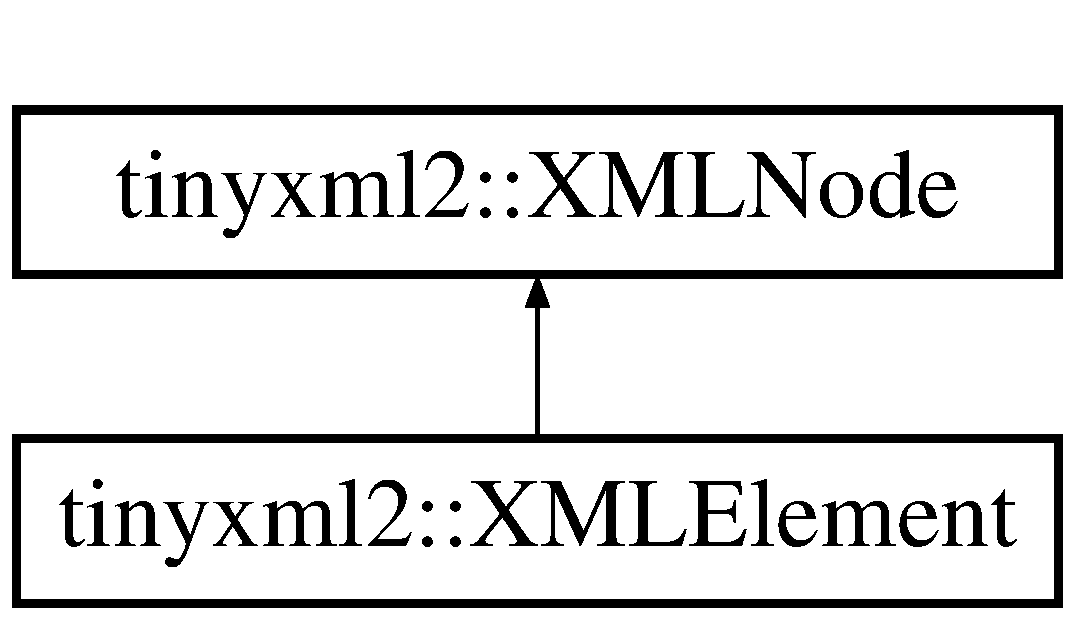
\includegraphics[height=2.000000cm]{classtinyxml2_1_1_x_m_l_element}
\end{center}
\end{figure}
\subsection*{Public Types}
\begin{DoxyCompactItemize}
\item 
\mbox{\Hypertarget{classtinyxml2_1_1_x_m_l_element_ab5f90e2493c35702175235127e2935b4}\label{classtinyxml2_1_1_x_m_l_element_ab5f90e2493c35702175235127e2935b4}} 
enum {\bfseries Element\+Closing\+Type} \{ {\bfseries O\+P\+EN}, 
{\bfseries C\+L\+O\+S\+ED}, 
{\bfseries C\+L\+O\+S\+I\+NG}
 \}
\end{DoxyCompactItemize}
\subsection*{Public Member Functions}
\begin{DoxyCompactItemize}
\item 
\mbox{\Hypertarget{classtinyxml2_1_1_x_m_l_element_a63e057fb5baee1dd29f323cb85907b35}\label{classtinyxml2_1_1_x_m_l_element_a63e057fb5baee1dd29f323cb85907b35}} 
const char $\ast$ \mbox{\hyperlink{classtinyxml2_1_1_x_m_l_element_a63e057fb5baee1dd29f323cb85907b35}{Name}} () const
\begin{DoxyCompactList}\small\item\em Get the name of an element (which is the \mbox{\hyperlink{classtinyxml2_1_1_x_m_l_node_a0485e51c670e741884cfd8362274d680}{Value()}} of the node.) \end{DoxyCompactList}\item 
\mbox{\Hypertarget{classtinyxml2_1_1_x_m_l_element_a97712009a530d8cb8a63bf705f02b4f1}\label{classtinyxml2_1_1_x_m_l_element_a97712009a530d8cb8a63bf705f02b4f1}} 
void \mbox{\hyperlink{classtinyxml2_1_1_x_m_l_element_a97712009a530d8cb8a63bf705f02b4f1}{Set\+Name}} (const char $\ast$str, bool static\+Mem=false)
\begin{DoxyCompactList}\small\item\em Set the name of the element. \end{DoxyCompactList}\item 
\mbox{\Hypertarget{classtinyxml2_1_1_x_m_l_element_ad9ff5c2dbc15df36cf664ce1b0ea0a5d}\label{classtinyxml2_1_1_x_m_l_element_ad9ff5c2dbc15df36cf664ce1b0ea0a5d}} 
virtual \mbox{\hyperlink{classtinyxml2_1_1_x_m_l_element}{X\+M\+L\+Element}} $\ast$ \mbox{\hyperlink{classtinyxml2_1_1_x_m_l_element_ad9ff5c2dbc15df36cf664ce1b0ea0a5d}{To\+Element}} ()
\begin{DoxyCompactList}\small\item\em Safely cast to an Element, or null. \end{DoxyCompactList}\item 
\mbox{\Hypertarget{classtinyxml2_1_1_x_m_l_element_afeb353047ab8532191709dcaef07337e}\label{classtinyxml2_1_1_x_m_l_element_afeb353047ab8532191709dcaef07337e}} 
virtual const \mbox{\hyperlink{classtinyxml2_1_1_x_m_l_element}{X\+M\+L\+Element}} $\ast$ {\bfseries To\+Element} () const
\item 
virtual bool \mbox{\hyperlink{classtinyxml2_1_1_x_m_l_element_a9b2119831e8b85827d5d3e5076788e4a}{Accept}} (\mbox{\hyperlink{classtinyxml2_1_1_x_m_l_visitor}{X\+M\+L\+Visitor}} $\ast$visitor) const
\item 
const char $\ast$ \mbox{\hyperlink{classtinyxml2_1_1_x_m_l_element_a48cf4a315cfbac7d74cd0d5ff2c5df51}{Attribute}} (const char $\ast$name, const char $\ast$value=0) const
\item 
int \mbox{\hyperlink{classtinyxml2_1_1_x_m_l_element_a95a89b13bb14a2d4655e2b5b406c00d4}{Int\+Attribute}} (const char $\ast$name, int default\+Value=0) const
\item 
\mbox{\Hypertarget{classtinyxml2_1_1_x_m_l_element_afea43a1d4aa33e3703ddee5fc9adc26c}\label{classtinyxml2_1_1_x_m_l_element_afea43a1d4aa33e3703ddee5fc9adc26c}} 
unsigned \mbox{\hyperlink{classtinyxml2_1_1_x_m_l_element_afea43a1d4aa33e3703ddee5fc9adc26c}{Unsigned\+Attribute}} (const char $\ast$name, unsigned default\+Value=0) const
\begin{DoxyCompactList}\small\item\em See \mbox{\hyperlink{classtinyxml2_1_1_x_m_l_element_a95a89b13bb14a2d4655e2b5b406c00d4}{Int\+Attribute()}} \end{DoxyCompactList}\item 
\mbox{\Hypertarget{classtinyxml2_1_1_x_m_l_element_a66d96972adecd816194191f13cc4a0a0}\label{classtinyxml2_1_1_x_m_l_element_a66d96972adecd816194191f13cc4a0a0}} 
int64\+\_\+t \mbox{\hyperlink{classtinyxml2_1_1_x_m_l_element_a66d96972adecd816194191f13cc4a0a0}{Int64\+Attribute}} (const char $\ast$name, int64\+\_\+t default\+Value=0) const
\begin{DoxyCompactList}\small\item\em See \mbox{\hyperlink{classtinyxml2_1_1_x_m_l_element_a95a89b13bb14a2d4655e2b5b406c00d4}{Int\+Attribute()}} \end{DoxyCompactList}\item 
\mbox{\Hypertarget{classtinyxml2_1_1_x_m_l_element_a53eda26131e1ad1031ef8ec8adb51bd8}\label{classtinyxml2_1_1_x_m_l_element_a53eda26131e1ad1031ef8ec8adb51bd8}} 
bool \mbox{\hyperlink{classtinyxml2_1_1_x_m_l_element_a53eda26131e1ad1031ef8ec8adb51bd8}{Bool\+Attribute}} (const char $\ast$name, bool default\+Value=false) const
\begin{DoxyCompactList}\small\item\em See \mbox{\hyperlink{classtinyxml2_1_1_x_m_l_element_a95a89b13bb14a2d4655e2b5b406c00d4}{Int\+Attribute()}} \end{DoxyCompactList}\item 
\mbox{\Hypertarget{classtinyxml2_1_1_x_m_l_element_a10a90c505aea716bf073eea1c97f33b5}\label{classtinyxml2_1_1_x_m_l_element_a10a90c505aea716bf073eea1c97f33b5}} 
double \mbox{\hyperlink{classtinyxml2_1_1_x_m_l_element_a10a90c505aea716bf073eea1c97f33b5}{Double\+Attribute}} (const char $\ast$name, double default\+Value=0) const
\begin{DoxyCompactList}\small\item\em See \mbox{\hyperlink{classtinyxml2_1_1_x_m_l_element_a95a89b13bb14a2d4655e2b5b406c00d4}{Int\+Attribute()}} \end{DoxyCompactList}\item 
\mbox{\Hypertarget{classtinyxml2_1_1_x_m_l_element_ab1f4be2332e27dc640e9b6abd01d64dd}\label{classtinyxml2_1_1_x_m_l_element_ab1f4be2332e27dc640e9b6abd01d64dd}} 
float \mbox{\hyperlink{classtinyxml2_1_1_x_m_l_element_ab1f4be2332e27dc640e9b6abd01d64dd}{Float\+Attribute}} (const char $\ast$name, float default\+Value=0) const
\begin{DoxyCompactList}\small\item\em See \mbox{\hyperlink{classtinyxml2_1_1_x_m_l_element_a95a89b13bb14a2d4655e2b5b406c00d4}{Int\+Attribute()}} \end{DoxyCompactList}\item 
X\+M\+L\+Error \mbox{\hyperlink{classtinyxml2_1_1_x_m_l_element_a8a78bc1187c1c45ad89f2690eab567b1}{Query\+Int\+Attribute}} (const char $\ast$name, int $\ast$value) const
\item 
\mbox{\Hypertarget{classtinyxml2_1_1_x_m_l_element_a26fc84cbfba6769dafcfbf256c05e22f}\label{classtinyxml2_1_1_x_m_l_element_a26fc84cbfba6769dafcfbf256c05e22f}} 
X\+M\+L\+Error \mbox{\hyperlink{classtinyxml2_1_1_x_m_l_element_a26fc84cbfba6769dafcfbf256c05e22f}{Query\+Unsigned\+Attribute}} (const char $\ast$name, unsigned int $\ast$value) const
\begin{DoxyCompactList}\small\item\em See \mbox{\hyperlink{classtinyxml2_1_1_x_m_l_element_a8a78bc1187c1c45ad89f2690eab567b1}{Query\+Int\+Attribute()}} \end{DoxyCompactList}\item 
\mbox{\Hypertarget{classtinyxml2_1_1_x_m_l_element_a7c0955d80b6f8d196744eacb0f6e90a8}\label{classtinyxml2_1_1_x_m_l_element_a7c0955d80b6f8d196744eacb0f6e90a8}} 
X\+M\+L\+Error \mbox{\hyperlink{classtinyxml2_1_1_x_m_l_element_a7c0955d80b6f8d196744eacb0f6e90a8}{Query\+Int64\+Attribute}} (const char $\ast$name, int64\+\_\+t $\ast$value) const
\begin{DoxyCompactList}\small\item\em See \mbox{\hyperlink{classtinyxml2_1_1_x_m_l_element_a8a78bc1187c1c45ad89f2690eab567b1}{Query\+Int\+Attribute()}} \end{DoxyCompactList}\item 
\mbox{\Hypertarget{classtinyxml2_1_1_x_m_l_element_a14c1bb77c39689838be01838d86ca872}\label{classtinyxml2_1_1_x_m_l_element_a14c1bb77c39689838be01838d86ca872}} 
X\+M\+L\+Error \mbox{\hyperlink{classtinyxml2_1_1_x_m_l_element_a14c1bb77c39689838be01838d86ca872}{Query\+Bool\+Attribute}} (const char $\ast$name, bool $\ast$value) const
\begin{DoxyCompactList}\small\item\em See \mbox{\hyperlink{classtinyxml2_1_1_x_m_l_element_a8a78bc1187c1c45ad89f2690eab567b1}{Query\+Int\+Attribute()}} \end{DoxyCompactList}\item 
\mbox{\Hypertarget{classtinyxml2_1_1_x_m_l_element_a5f0964e2dbd8e2ee7fce9beab689443c}\label{classtinyxml2_1_1_x_m_l_element_a5f0964e2dbd8e2ee7fce9beab689443c}} 
X\+M\+L\+Error \mbox{\hyperlink{classtinyxml2_1_1_x_m_l_element_a5f0964e2dbd8e2ee7fce9beab689443c}{Query\+Double\+Attribute}} (const char $\ast$name, double $\ast$value) const
\begin{DoxyCompactList}\small\item\em See \mbox{\hyperlink{classtinyxml2_1_1_x_m_l_element_a8a78bc1187c1c45ad89f2690eab567b1}{Query\+Int\+Attribute()}} \end{DoxyCompactList}\item 
\mbox{\Hypertarget{classtinyxml2_1_1_x_m_l_element_acd5eeddf6002ef90806af794b9d9a5a5}\label{classtinyxml2_1_1_x_m_l_element_acd5eeddf6002ef90806af794b9d9a5a5}} 
X\+M\+L\+Error \mbox{\hyperlink{classtinyxml2_1_1_x_m_l_element_acd5eeddf6002ef90806af794b9d9a5a5}{Query\+Float\+Attribute}} (const char $\ast$name, float $\ast$value) const
\begin{DoxyCompactList}\small\item\em See \mbox{\hyperlink{classtinyxml2_1_1_x_m_l_element_a8a78bc1187c1c45ad89f2690eab567b1}{Query\+Int\+Attribute()}} \end{DoxyCompactList}\item 
\mbox{\Hypertarget{classtinyxml2_1_1_x_m_l_element_adb8ae765f98d0c5037faec48deea78bc}\label{classtinyxml2_1_1_x_m_l_element_adb8ae765f98d0c5037faec48deea78bc}} 
X\+M\+L\+Error \mbox{\hyperlink{classtinyxml2_1_1_x_m_l_element_adb8ae765f98d0c5037faec48deea78bc}{Query\+String\+Attribute}} (const char $\ast$name, const char $\ast$$\ast$value) const
\begin{DoxyCompactList}\small\item\em See \mbox{\hyperlink{classtinyxml2_1_1_x_m_l_element_a8a78bc1187c1c45ad89f2690eab567b1}{Query\+Int\+Attribute()}} \end{DoxyCompactList}\item 
int \mbox{\hyperlink{classtinyxml2_1_1_x_m_l_element_a042fc30504347b84a56cf863ad528a4f}{Query\+Attribute}} (const char $\ast$name, int $\ast$value) const
\item 
\mbox{\Hypertarget{classtinyxml2_1_1_x_m_l_element_a187e8b686fbe071732aea2e2ee766f86}\label{classtinyxml2_1_1_x_m_l_element_a187e8b686fbe071732aea2e2ee766f86}} 
int {\bfseries Query\+Attribute} (const char $\ast$name, unsigned int $\ast$value) const
\item 
\mbox{\Hypertarget{classtinyxml2_1_1_x_m_l_element_aedcac9a0842cc9fcb49ba6eee4dd47bc}\label{classtinyxml2_1_1_x_m_l_element_aedcac9a0842cc9fcb49ba6eee4dd47bc}} 
int {\bfseries Query\+Attribute} (const char $\ast$name, int64\+\_\+t $\ast$value) const
\item 
\mbox{\Hypertarget{classtinyxml2_1_1_x_m_l_element_a9aa67feb0392ead13a66f5ea55e71f64}\label{classtinyxml2_1_1_x_m_l_element_a9aa67feb0392ead13a66f5ea55e71f64}} 
int {\bfseries Query\+Attribute} (const char $\ast$name, bool $\ast$value) const
\item 
\mbox{\Hypertarget{classtinyxml2_1_1_x_m_l_element_a7f37582f3ad9f9a765e6fa349dfbdfa0}\label{classtinyxml2_1_1_x_m_l_element_a7f37582f3ad9f9a765e6fa349dfbdfa0}} 
int {\bfseries Query\+Attribute} (const char $\ast$name, double $\ast$value) const
\item 
\mbox{\Hypertarget{classtinyxml2_1_1_x_m_l_element_a493b6dace830e4dba7110b1e9f6bebd5}\label{classtinyxml2_1_1_x_m_l_element_a493b6dace830e4dba7110b1e9f6bebd5}} 
int {\bfseries Query\+Attribute} (const char $\ast$name, float $\ast$value) const
\item 
\mbox{\Hypertarget{classtinyxml2_1_1_x_m_l_element_a11943abf2d0831548c3790dd5d9f119c}\label{classtinyxml2_1_1_x_m_l_element_a11943abf2d0831548c3790dd5d9f119c}} 
void \mbox{\hyperlink{classtinyxml2_1_1_x_m_l_element_a11943abf2d0831548c3790dd5d9f119c}{Set\+Attribute}} (const char $\ast$name, const char $\ast$value)
\begin{DoxyCompactList}\small\item\em Sets the named attribute to value. \end{DoxyCompactList}\item 
\mbox{\Hypertarget{classtinyxml2_1_1_x_m_l_element_aae6568c64c7f1cc88be8461ba41a79cf}\label{classtinyxml2_1_1_x_m_l_element_aae6568c64c7f1cc88be8461ba41a79cf}} 
void \mbox{\hyperlink{classtinyxml2_1_1_x_m_l_element_aae6568c64c7f1cc88be8461ba41a79cf}{Set\+Attribute}} (const char $\ast$name, int value)
\begin{DoxyCompactList}\small\item\em Sets the named attribute to value. \end{DoxyCompactList}\item 
\mbox{\Hypertarget{classtinyxml2_1_1_x_m_l_element_ae143997e90064ba82326b29a9930ea8f}\label{classtinyxml2_1_1_x_m_l_element_ae143997e90064ba82326b29a9930ea8f}} 
void \mbox{\hyperlink{classtinyxml2_1_1_x_m_l_element_ae143997e90064ba82326b29a9930ea8f}{Set\+Attribute}} (const char $\ast$name, unsigned value)
\begin{DoxyCompactList}\small\item\em Sets the named attribute to value. \end{DoxyCompactList}\item 
\mbox{\Hypertarget{classtinyxml2_1_1_x_m_l_element_aaeefdf9171fec91b13a776b42299b0dd}\label{classtinyxml2_1_1_x_m_l_element_aaeefdf9171fec91b13a776b42299b0dd}} 
void \mbox{\hyperlink{classtinyxml2_1_1_x_m_l_element_aaeefdf9171fec91b13a776b42299b0dd}{Set\+Attribute}} (const char $\ast$name, int64\+\_\+t value)
\begin{DoxyCompactList}\small\item\em Sets the named attribute to value. \end{DoxyCompactList}\item 
\mbox{\Hypertarget{classtinyxml2_1_1_x_m_l_element_aa848b696e6a75e4e545c6da9893b11e1}\label{classtinyxml2_1_1_x_m_l_element_aa848b696e6a75e4e545c6da9893b11e1}} 
void \mbox{\hyperlink{classtinyxml2_1_1_x_m_l_element_aa848b696e6a75e4e545c6da9893b11e1}{Set\+Attribute}} (const char $\ast$name, bool value)
\begin{DoxyCompactList}\small\item\em Sets the named attribute to value. \end{DoxyCompactList}\item 
\mbox{\Hypertarget{classtinyxml2_1_1_x_m_l_element_a233397ee81e70eb5d4b814c5f8698533}\label{classtinyxml2_1_1_x_m_l_element_a233397ee81e70eb5d4b814c5f8698533}} 
void \mbox{\hyperlink{classtinyxml2_1_1_x_m_l_element_a233397ee81e70eb5d4b814c5f8698533}{Set\+Attribute}} (const char $\ast$name, double value)
\begin{DoxyCompactList}\small\item\em Sets the named attribute to value. \end{DoxyCompactList}\item 
\mbox{\Hypertarget{classtinyxml2_1_1_x_m_l_element_a554b70d882e65b28fc084b23df9b9759}\label{classtinyxml2_1_1_x_m_l_element_a554b70d882e65b28fc084b23df9b9759}} 
void \mbox{\hyperlink{classtinyxml2_1_1_x_m_l_element_a554b70d882e65b28fc084b23df9b9759}{Set\+Attribute}} (const char $\ast$name, float value)
\begin{DoxyCompactList}\small\item\em Sets the named attribute to value. \end{DoxyCompactList}\item 
void \mbox{\hyperlink{classtinyxml2_1_1_x_m_l_element_aebd45aa7118964c30b32fe12e944628a}{Delete\+Attribute}} (const char $\ast$name)
\item 
\mbox{\Hypertarget{classtinyxml2_1_1_x_m_l_element_a3e191704c8d499906ec11fe2f60c6686}\label{classtinyxml2_1_1_x_m_l_element_a3e191704c8d499906ec11fe2f60c6686}} 
const \mbox{\hyperlink{classtinyxml2_1_1_x_m_l_attribute}{X\+M\+L\+Attribute}} $\ast$ \mbox{\hyperlink{classtinyxml2_1_1_x_m_l_element_a3e191704c8d499906ec11fe2f60c6686}{First\+Attribute}} () const
\begin{DoxyCompactList}\small\item\em Return the first attribute in the list. \end{DoxyCompactList}\item 
\mbox{\Hypertarget{classtinyxml2_1_1_x_m_l_element_a157750dac8037a316fd1af1a973dfa2c}\label{classtinyxml2_1_1_x_m_l_element_a157750dac8037a316fd1af1a973dfa2c}} 
const \mbox{\hyperlink{classtinyxml2_1_1_x_m_l_attribute}{X\+M\+L\+Attribute}} $\ast$ \mbox{\hyperlink{classtinyxml2_1_1_x_m_l_element_a157750dac8037a316fd1af1a973dfa2c}{Find\+Attribute}} (const char $\ast$name) const
\begin{DoxyCompactList}\small\item\em Query a specific attribute in the list. \end{DoxyCompactList}\item 
const char $\ast$ \mbox{\hyperlink{classtinyxml2_1_1_x_m_l_element_a0fa5bea0a4daf3ddd503dcabb823eba6}{Get\+Text}} () const
\item 
void \mbox{\hyperlink{classtinyxml2_1_1_x_m_l_element_a1f9c2cd61b72af5ae708d37b7ad283ce}{Set\+Text}} (const char $\ast$in\+Text)
\item 
\mbox{\Hypertarget{classtinyxml2_1_1_x_m_l_element_aeae8917b5ea6060b3c08d4e3d8d632d7}\label{classtinyxml2_1_1_x_m_l_element_aeae8917b5ea6060b3c08d4e3d8d632d7}} 
void \mbox{\hyperlink{classtinyxml2_1_1_x_m_l_element_aeae8917b5ea6060b3c08d4e3d8d632d7}{Set\+Text}} (int value)
\begin{DoxyCompactList}\small\item\em Convenience method for setting text inside an element. See \mbox{\hyperlink{classtinyxml2_1_1_x_m_l_element_a1f9c2cd61b72af5ae708d37b7ad283ce}{Set\+Text()}} for important limitations. \end{DoxyCompactList}\item 
\mbox{\Hypertarget{classtinyxml2_1_1_x_m_l_element_a7bbfcc11d516598bc924a8fba4d08597}\label{classtinyxml2_1_1_x_m_l_element_a7bbfcc11d516598bc924a8fba4d08597}} 
void \mbox{\hyperlink{classtinyxml2_1_1_x_m_l_element_a7bbfcc11d516598bc924a8fba4d08597}{Set\+Text}} (unsigned value)
\begin{DoxyCompactList}\small\item\em Convenience method for setting text inside an element. See \mbox{\hyperlink{classtinyxml2_1_1_x_m_l_element_a1f9c2cd61b72af5ae708d37b7ad283ce}{Set\+Text()}} for important limitations. \end{DoxyCompactList}\item 
\mbox{\Hypertarget{classtinyxml2_1_1_x_m_l_element_a7b62cd33acdfeff7ea2b1b330d4368e4}\label{classtinyxml2_1_1_x_m_l_element_a7b62cd33acdfeff7ea2b1b330d4368e4}} 
void \mbox{\hyperlink{classtinyxml2_1_1_x_m_l_element_a7b62cd33acdfeff7ea2b1b330d4368e4}{Set\+Text}} (int64\+\_\+t value)
\begin{DoxyCompactList}\small\item\em Convenience method for setting text inside an element. See \mbox{\hyperlink{classtinyxml2_1_1_x_m_l_element_a1f9c2cd61b72af5ae708d37b7ad283ce}{Set\+Text()}} for important limitations. \end{DoxyCompactList}\item 
\mbox{\Hypertarget{classtinyxml2_1_1_x_m_l_element_ae4b543d6770de76fb6ab68e541c192a4}\label{classtinyxml2_1_1_x_m_l_element_ae4b543d6770de76fb6ab68e541c192a4}} 
void \mbox{\hyperlink{classtinyxml2_1_1_x_m_l_element_ae4b543d6770de76fb6ab68e541c192a4}{Set\+Text}} (bool value)
\begin{DoxyCompactList}\small\item\em Convenience method for setting text inside an element. See \mbox{\hyperlink{classtinyxml2_1_1_x_m_l_element_a1f9c2cd61b72af5ae708d37b7ad283ce}{Set\+Text()}} for important limitations. \end{DoxyCompactList}\item 
\mbox{\Hypertarget{classtinyxml2_1_1_x_m_l_element_a67bd77ac9aaeff58ff20b4275a65ba4e}\label{classtinyxml2_1_1_x_m_l_element_a67bd77ac9aaeff58ff20b4275a65ba4e}} 
void \mbox{\hyperlink{classtinyxml2_1_1_x_m_l_element_a67bd77ac9aaeff58ff20b4275a65ba4e}{Set\+Text}} (double value)
\begin{DoxyCompactList}\small\item\em Convenience method for setting text inside an element. See \mbox{\hyperlink{classtinyxml2_1_1_x_m_l_element_a1f9c2cd61b72af5ae708d37b7ad283ce}{Set\+Text()}} for important limitations. \end{DoxyCompactList}\item 
\mbox{\Hypertarget{classtinyxml2_1_1_x_m_l_element_a51d560da5ae3ad6b75e0ab9ffb2ae42a}\label{classtinyxml2_1_1_x_m_l_element_a51d560da5ae3ad6b75e0ab9ffb2ae42a}} 
void \mbox{\hyperlink{classtinyxml2_1_1_x_m_l_element_a51d560da5ae3ad6b75e0ab9ffb2ae42a}{Set\+Text}} (float value)
\begin{DoxyCompactList}\small\item\em Convenience method for setting text inside an element. See \mbox{\hyperlink{classtinyxml2_1_1_x_m_l_element_a1f9c2cd61b72af5ae708d37b7ad283ce}{Set\+Text()}} for important limitations. \end{DoxyCompactList}\item 
X\+M\+L\+Error \mbox{\hyperlink{classtinyxml2_1_1_x_m_l_element_a926357996bef633cb736e1a558419632}{Query\+Int\+Text}} (int $\ast$ival) const
\item 
\mbox{\Hypertarget{classtinyxml2_1_1_x_m_l_element_a14d38aa4b5e18a46274a27425188a6a1}\label{classtinyxml2_1_1_x_m_l_element_a14d38aa4b5e18a46274a27425188a6a1}} 
X\+M\+L\+Error \mbox{\hyperlink{classtinyxml2_1_1_x_m_l_element_a14d38aa4b5e18a46274a27425188a6a1}{Query\+Unsigned\+Text}} (unsigned $\ast$uval) const
\begin{DoxyCompactList}\small\item\em See \mbox{\hyperlink{classtinyxml2_1_1_x_m_l_element_a926357996bef633cb736e1a558419632}{Query\+Int\+Text()}} \end{DoxyCompactList}\item 
\mbox{\Hypertarget{classtinyxml2_1_1_x_m_l_element_a120c538c8eead169e635dbc70fb226d8}\label{classtinyxml2_1_1_x_m_l_element_a120c538c8eead169e635dbc70fb226d8}} 
X\+M\+L\+Error \mbox{\hyperlink{classtinyxml2_1_1_x_m_l_element_a120c538c8eead169e635dbc70fb226d8}{Query\+Int64\+Text}} (int64\+\_\+t $\ast$uval) const
\begin{DoxyCompactList}\small\item\em See \mbox{\hyperlink{classtinyxml2_1_1_x_m_l_element_a926357996bef633cb736e1a558419632}{Query\+Int\+Text()}} \end{DoxyCompactList}\item 
\mbox{\Hypertarget{classtinyxml2_1_1_x_m_l_element_a3fe5417d59eb8f5c4afe924b7d332736}\label{classtinyxml2_1_1_x_m_l_element_a3fe5417d59eb8f5c4afe924b7d332736}} 
X\+M\+L\+Error \mbox{\hyperlink{classtinyxml2_1_1_x_m_l_element_a3fe5417d59eb8f5c4afe924b7d332736}{Query\+Bool\+Text}} (bool $\ast$bval) const
\begin{DoxyCompactList}\small\item\em See \mbox{\hyperlink{classtinyxml2_1_1_x_m_l_element_a926357996bef633cb736e1a558419632}{Query\+Int\+Text()}} \end{DoxyCompactList}\item 
\mbox{\Hypertarget{classtinyxml2_1_1_x_m_l_element_a684679c99bb036a25652744cec6c4d96}\label{classtinyxml2_1_1_x_m_l_element_a684679c99bb036a25652744cec6c4d96}} 
X\+M\+L\+Error \mbox{\hyperlink{classtinyxml2_1_1_x_m_l_element_a684679c99bb036a25652744cec6c4d96}{Query\+Double\+Text}} (double $\ast$dval) const
\begin{DoxyCompactList}\small\item\em See \mbox{\hyperlink{classtinyxml2_1_1_x_m_l_element_a926357996bef633cb736e1a558419632}{Query\+Int\+Text()}} \end{DoxyCompactList}\item 
\mbox{\Hypertarget{classtinyxml2_1_1_x_m_l_element_afa332afedd93210daa6d44b88eb11e29}\label{classtinyxml2_1_1_x_m_l_element_afa332afedd93210daa6d44b88eb11e29}} 
X\+M\+L\+Error \mbox{\hyperlink{classtinyxml2_1_1_x_m_l_element_afa332afedd93210daa6d44b88eb11e29}{Query\+Float\+Text}} (float $\ast$fval) const
\begin{DoxyCompactList}\small\item\em See \mbox{\hyperlink{classtinyxml2_1_1_x_m_l_element_a926357996bef633cb736e1a558419632}{Query\+Int\+Text()}} \end{DoxyCompactList}\item 
\mbox{\Hypertarget{classtinyxml2_1_1_x_m_l_element_a37b0636adebb8a1a1bc965f60824cb3e}\label{classtinyxml2_1_1_x_m_l_element_a37b0636adebb8a1a1bc965f60824cb3e}} 
int {\bfseries Int\+Text} (int default\+Value=0) const
\item 
\mbox{\Hypertarget{classtinyxml2_1_1_x_m_l_element_a49bad014ffcc17b0b6119d5b2c97dfb5}\label{classtinyxml2_1_1_x_m_l_element_a49bad014ffcc17b0b6119d5b2c97dfb5}} 
unsigned \mbox{\hyperlink{classtinyxml2_1_1_x_m_l_element_a49bad014ffcc17b0b6119d5b2c97dfb5}{Unsigned\+Text}} (unsigned default\+Value=0) const
\begin{DoxyCompactList}\small\item\em See \mbox{\hyperlink{classtinyxml2_1_1_x_m_l_element_a926357996bef633cb736e1a558419632}{Query\+Int\+Text()}} \end{DoxyCompactList}\item 
\mbox{\Hypertarget{classtinyxml2_1_1_x_m_l_element_aab6151f7e3b4c2c0a8234e262d7b6b8a}\label{classtinyxml2_1_1_x_m_l_element_aab6151f7e3b4c2c0a8234e262d7b6b8a}} 
int64\+\_\+t \mbox{\hyperlink{classtinyxml2_1_1_x_m_l_element_aab6151f7e3b4c2c0a8234e262d7b6b8a}{Int64\+Text}} (int64\+\_\+t default\+Value=0) const
\begin{DoxyCompactList}\small\item\em See \mbox{\hyperlink{classtinyxml2_1_1_x_m_l_element_a926357996bef633cb736e1a558419632}{Query\+Int\+Text()}} \end{DoxyCompactList}\item 
\mbox{\Hypertarget{classtinyxml2_1_1_x_m_l_element_a68569f59f6382bcea7f5013ec59736d2}\label{classtinyxml2_1_1_x_m_l_element_a68569f59f6382bcea7f5013ec59736d2}} 
bool \mbox{\hyperlink{classtinyxml2_1_1_x_m_l_element_a68569f59f6382bcea7f5013ec59736d2}{Bool\+Text}} (bool default\+Value=false) const
\begin{DoxyCompactList}\small\item\em See \mbox{\hyperlink{classtinyxml2_1_1_x_m_l_element_a926357996bef633cb736e1a558419632}{Query\+Int\+Text()}} \end{DoxyCompactList}\item 
\mbox{\Hypertarget{classtinyxml2_1_1_x_m_l_element_a81b1ff0cf2f2cd09be8badc08b39a2b7}\label{classtinyxml2_1_1_x_m_l_element_a81b1ff0cf2f2cd09be8badc08b39a2b7}} 
double \mbox{\hyperlink{classtinyxml2_1_1_x_m_l_element_a81b1ff0cf2f2cd09be8badc08b39a2b7}{Double\+Text}} (double default\+Value=0) const
\begin{DoxyCompactList}\small\item\em See \mbox{\hyperlink{classtinyxml2_1_1_x_m_l_element_a926357996bef633cb736e1a558419632}{Query\+Int\+Text()}} \end{DoxyCompactList}\item 
\mbox{\Hypertarget{classtinyxml2_1_1_x_m_l_element_a45444eb21f99ca46101545992dc2e927}\label{classtinyxml2_1_1_x_m_l_element_a45444eb21f99ca46101545992dc2e927}} 
float \mbox{\hyperlink{classtinyxml2_1_1_x_m_l_element_a45444eb21f99ca46101545992dc2e927}{Float\+Text}} (float default\+Value=0) const
\begin{DoxyCompactList}\small\item\em See \mbox{\hyperlink{classtinyxml2_1_1_x_m_l_element_a926357996bef633cb736e1a558419632}{Query\+Int\+Text()}} \end{DoxyCompactList}\item 
\mbox{\Hypertarget{classtinyxml2_1_1_x_m_l_element_a6965ff89557f27d4082d7043d5145555}\label{classtinyxml2_1_1_x_m_l_element_a6965ff89557f27d4082d7043d5145555}} 
Element\+Closing\+Type {\bfseries Closing\+Type} () const
\item 
virtual \mbox{\hyperlink{classtinyxml2_1_1_x_m_l_node}{X\+M\+L\+Node}} $\ast$ \mbox{\hyperlink{classtinyxml2_1_1_x_m_l_element_aafa2807a45b28fe096b29d76e6a13b7c}{Shallow\+Clone}} (\mbox{\hyperlink{classtinyxml2_1_1_x_m_l_document}{X\+M\+L\+Document}} $\ast$document) const
\item 
virtual bool \mbox{\hyperlink{classtinyxml2_1_1_x_m_l_element_a61ffd7bf918a9db4aa6203d855ac5ec2}{Shallow\+Equal}} (const \mbox{\hyperlink{classtinyxml2_1_1_x_m_l_node}{X\+M\+L\+Node}} $\ast$compare) const
\end{DoxyCompactItemize}
\subsection*{Protected Member Functions}
\begin{DoxyCompactItemize}
\item 
\mbox{\Hypertarget{classtinyxml2_1_1_x_m_l_element_a072998100b7d0ba5e8aeac6dd6dfb31b}\label{classtinyxml2_1_1_x_m_l_element_a072998100b7d0ba5e8aeac6dd6dfb31b}} 
char $\ast$ {\bfseries Parse\+Deep} (char $\ast$p, \mbox{\hyperlink{classtinyxml2_1_1_str_pair}{Str\+Pair}} $\ast$parent\+End\+Tag, int $\ast$cur\+Line\+Num\+Ptr)
\end{DoxyCompactItemize}
\subsection*{Friends}
\begin{DoxyCompactItemize}
\item 
\mbox{\Hypertarget{classtinyxml2_1_1_x_m_l_element_a4eee3bda60c60a30e4e8cd4ea91c4c6e}\label{classtinyxml2_1_1_x_m_l_element_a4eee3bda60c60a30e4e8cd4ea91c4c6e}} 
class {\bfseries X\+M\+L\+Document}
\end{DoxyCompactItemize}
\subsection*{Additional Inherited Members}


\subsection{Detailed Description}
The element is a container class. It has a value, the element name, and can contain other elements, text, comments, and unknowns. Elements also contain an arbitrary number of attributes. 

\subsection{Member Function Documentation}
\mbox{\Hypertarget{classtinyxml2_1_1_x_m_l_element_a9b2119831e8b85827d5d3e5076788e4a}\label{classtinyxml2_1_1_x_m_l_element_a9b2119831e8b85827d5d3e5076788e4a}} 
\index{tinyxml2\+::\+X\+M\+L\+Element@{tinyxml2\+::\+X\+M\+L\+Element}!Accept@{Accept}}
\index{Accept@{Accept}!tinyxml2\+::\+X\+M\+L\+Element@{tinyxml2\+::\+X\+M\+L\+Element}}
\subsubsection{\texorpdfstring{Accept()}{Accept()}}
{\footnotesize\ttfamily bool tinyxml2\+::\+X\+M\+L\+Element\+::\+Accept (\begin{DoxyParamCaption}\item[{\mbox{\hyperlink{classtinyxml2_1_1_x_m_l_visitor}{X\+M\+L\+Visitor}} $\ast$}]{visitor }\end{DoxyParamCaption}) const\hspace{0.3cm}{\ttfamily [virtual]}}

Accept a hierarchical visit of the nodes in the Tiny\+X\+M\+L-\/2 D\+OM. Every node in the X\+ML tree will be conditionally visited and the host will be called back via the \mbox{\hyperlink{classtinyxml2_1_1_x_m_l_visitor}{X\+M\+L\+Visitor}} interface.

This is essentially a S\+AX interface for Tiny\+X\+M\+L-\/2. (Note however it doesn\textquotesingle{}t re-\/parse the X\+ML for the callbacks, so the performance of Tiny\+X\+M\+L-\/2 is unchanged by using this interface versus any other.)

The interface has been based on ideas from\+:


\begin{DoxyItemize}
\item \href{http://www.saxproject.org/}{\tt http\+://www.\+saxproject.\+org/}
\item \href{http://c2.com/cgi/wiki?HierarchicalVisitorPattern}{\tt http\+://c2.\+com/cgi/wiki?\+Hierarchical\+Visitor\+Pattern}
\end{DoxyItemize}

Which are both good references for \char`\"{}visiting\char`\"{}.

An example of using \mbox{\hyperlink{classtinyxml2_1_1_x_m_l_element_a9b2119831e8b85827d5d3e5076788e4a}{Accept()}}\+: \begin{DoxyVerb}XMLPrinter printer;
tinyxmlDoc.Accept( &printer );
const char* xmlcstr = printer.CStr();
\end{DoxyVerb}
 

Implements \mbox{\hyperlink{classtinyxml2_1_1_x_m_l_node_a81e66df0a44c67a7af17f3b77a152785}{tinyxml2\+::\+X\+M\+L\+Node}}.

\mbox{\Hypertarget{classtinyxml2_1_1_x_m_l_element_a48cf4a315cfbac7d74cd0d5ff2c5df51}\label{classtinyxml2_1_1_x_m_l_element_a48cf4a315cfbac7d74cd0d5ff2c5df51}} 
\index{tinyxml2\+::\+X\+M\+L\+Element@{tinyxml2\+::\+X\+M\+L\+Element}!Attribute@{Attribute}}
\index{Attribute@{Attribute}!tinyxml2\+::\+X\+M\+L\+Element@{tinyxml2\+::\+X\+M\+L\+Element}}
\subsubsection{\texorpdfstring{Attribute()}{Attribute()}}
{\footnotesize\ttfamily const char $\ast$ tinyxml2\+::\+X\+M\+L\+Element\+::\+Attribute (\begin{DoxyParamCaption}\item[{const char $\ast$}]{name,  }\item[{const char $\ast$}]{value = {\ttfamily 0} }\end{DoxyParamCaption}) const}

Given an attribute name, \mbox{\hyperlink{classtinyxml2_1_1_x_m_l_element_a48cf4a315cfbac7d74cd0d5ff2c5df51}{Attribute()}} returns the value for the attribute of that name, or null if none exists. For example\+:

\begin{DoxyVerb}const char* value = ele->Attribute( "foo" );
\end{DoxyVerb}


The \textquotesingle{}value\textquotesingle{} parameter is normally null. However, if specified, the attribute will only be returned if the \textquotesingle{}name\textquotesingle{} and \textquotesingle{}value\textquotesingle{} match. This allow you to write code\+:

\begin{DoxyVerb}if ( ele->Attribute( "foo", "bar" ) ) callFooIsBar();
\end{DoxyVerb}


rather than\+: \begin{DoxyVerb}if ( ele->Attribute( "foo" ) ) {
    if ( strcmp( ele->Attribute( "foo" ), "bar" ) == 0 ) callFooIsBar();
}
\end{DoxyVerb}
 \mbox{\Hypertarget{classtinyxml2_1_1_x_m_l_element_aebd45aa7118964c30b32fe12e944628a}\label{classtinyxml2_1_1_x_m_l_element_aebd45aa7118964c30b32fe12e944628a}} 
\index{tinyxml2\+::\+X\+M\+L\+Element@{tinyxml2\+::\+X\+M\+L\+Element}!Delete\+Attribute@{Delete\+Attribute}}
\index{Delete\+Attribute@{Delete\+Attribute}!tinyxml2\+::\+X\+M\+L\+Element@{tinyxml2\+::\+X\+M\+L\+Element}}
\subsubsection{\texorpdfstring{Delete\+Attribute()}{DeleteAttribute()}}
{\footnotesize\ttfamily void tinyxml2\+::\+X\+M\+L\+Element\+::\+Delete\+Attribute (\begin{DoxyParamCaption}\item[{const char $\ast$}]{name }\end{DoxyParamCaption})}

Delete an attribute. \mbox{\Hypertarget{classtinyxml2_1_1_x_m_l_element_a0fa5bea0a4daf3ddd503dcabb823eba6}\label{classtinyxml2_1_1_x_m_l_element_a0fa5bea0a4daf3ddd503dcabb823eba6}} 
\index{tinyxml2\+::\+X\+M\+L\+Element@{tinyxml2\+::\+X\+M\+L\+Element}!Get\+Text@{Get\+Text}}
\index{Get\+Text@{Get\+Text}!tinyxml2\+::\+X\+M\+L\+Element@{tinyxml2\+::\+X\+M\+L\+Element}}
\subsubsection{\texorpdfstring{Get\+Text()}{GetText()}}
{\footnotesize\ttfamily const char $\ast$ tinyxml2\+::\+X\+M\+L\+Element\+::\+Get\+Text (\begin{DoxyParamCaption}{ }\end{DoxyParamCaption}) const}

Convenience function for easy access to the text inside an element. Although easy and concise, \mbox{\hyperlink{classtinyxml2_1_1_x_m_l_element_a0fa5bea0a4daf3ddd503dcabb823eba6}{Get\+Text()}} is limited compared to getting the \mbox{\hyperlink{classtinyxml2_1_1_x_m_l_text}{X\+M\+L\+Text}} child and accessing it directly.

If the first child of \textquotesingle{}this\textquotesingle{} is a \mbox{\hyperlink{classtinyxml2_1_1_x_m_l_text}{X\+M\+L\+Text}}, the \mbox{\hyperlink{classtinyxml2_1_1_x_m_l_element_a0fa5bea0a4daf3ddd503dcabb823eba6}{Get\+Text()}} returns the character string of the Text node, else null is returned.

This is a convenient method for getting the text of simple contained text\+: \begin{DoxyVerb}<foo>This is text</foo>
    const char* str = fooElement->GetText();
\end{DoxyVerb}


\textquotesingle{}str\textquotesingle{} will be a pointer to \char`\"{}\+This is text\char`\"{}.

Note that this function can be misleading. If the element foo was created from this X\+ML\+: \begin{DoxyVerb}    <foo><b>This is text</b></foo>
\end{DoxyVerb}


then the value of str would be null. The first child node isn\textquotesingle{}t a text node, it is another element. From this X\+ML\+: \begin{DoxyVerb}    <foo>This is <b>text</b></foo>
\end{DoxyVerb}
 \mbox{\hyperlink{classtinyxml2_1_1_x_m_l_element_a0fa5bea0a4daf3ddd503dcabb823eba6}{Get\+Text()}} will return \char`\"{}\+This is \char`\"{}. \mbox{\Hypertarget{classtinyxml2_1_1_x_m_l_element_a95a89b13bb14a2d4655e2b5b406c00d4}\label{classtinyxml2_1_1_x_m_l_element_a95a89b13bb14a2d4655e2b5b406c00d4}} 
\index{tinyxml2\+::\+X\+M\+L\+Element@{tinyxml2\+::\+X\+M\+L\+Element}!Int\+Attribute@{Int\+Attribute}}
\index{Int\+Attribute@{Int\+Attribute}!tinyxml2\+::\+X\+M\+L\+Element@{tinyxml2\+::\+X\+M\+L\+Element}}
\subsubsection{\texorpdfstring{Int\+Attribute()}{IntAttribute()}}
{\footnotesize\ttfamily int tinyxml2\+::\+X\+M\+L\+Element\+::\+Int\+Attribute (\begin{DoxyParamCaption}\item[{const char $\ast$}]{name,  }\item[{int}]{default\+Value = {\ttfamily 0} }\end{DoxyParamCaption}) const}

Given an attribute name, \mbox{\hyperlink{classtinyxml2_1_1_x_m_l_element_a95a89b13bb14a2d4655e2b5b406c00d4}{Int\+Attribute()}} returns the value of the attribute interpreted as an integer. The default value will be returned if the attribute isn\textquotesingle{}t present, or if there is an error. (For a method with error checking, see \mbox{\hyperlink{classtinyxml2_1_1_x_m_l_element_a8a78bc1187c1c45ad89f2690eab567b1}{Query\+Int\+Attribute()}}). \mbox{\Hypertarget{classtinyxml2_1_1_x_m_l_element_a042fc30504347b84a56cf863ad528a4f}\label{classtinyxml2_1_1_x_m_l_element_a042fc30504347b84a56cf863ad528a4f}} 
\index{tinyxml2\+::\+X\+M\+L\+Element@{tinyxml2\+::\+X\+M\+L\+Element}!Query\+Attribute@{Query\+Attribute}}
\index{Query\+Attribute@{Query\+Attribute}!tinyxml2\+::\+X\+M\+L\+Element@{tinyxml2\+::\+X\+M\+L\+Element}}
\subsubsection{\texorpdfstring{Query\+Attribute()}{QueryAttribute()}}
{\footnotesize\ttfamily int tinyxml2\+::\+X\+M\+L\+Element\+::\+Query\+Attribute (\begin{DoxyParamCaption}\item[{const char $\ast$}]{name,  }\item[{int $\ast$}]{value }\end{DoxyParamCaption}) const\hspace{0.3cm}{\ttfamily [inline]}}

Given an attribute name, \mbox{\hyperlink{classtinyxml2_1_1_x_m_l_element_a042fc30504347b84a56cf863ad528a4f}{Query\+Attribute()}} returns X\+M\+L\+\_\+\+S\+U\+C\+C\+E\+SS, X\+M\+L\+\_\+\+W\+R\+O\+N\+G\+\_\+\+A\+T\+T\+R\+I\+B\+U\+T\+E\+\_\+\+T\+Y\+PE if the conversion can\textquotesingle{}t be performed, or X\+M\+L\+\_\+\+N\+O\+\_\+\+A\+T\+T\+R\+I\+B\+U\+TE if the attribute doesn\textquotesingle{}t exist. It is overloaded for the primitive types, and is a generally more convenient replacement of \mbox{\hyperlink{classtinyxml2_1_1_x_m_l_element_a8a78bc1187c1c45ad89f2690eab567b1}{Query\+Int\+Attribute()}} and related functions.

If successful, the result of the conversion will be written to \textquotesingle{}value\textquotesingle{}. If not successful, nothing will be written to \textquotesingle{}value\textquotesingle{}. This allows you to provide default value\+:

\begin{DoxyVerb}int value = 10;
QueryAttribute( "foo", &value );        // if "foo" isn't found, value will still be 10
\end{DoxyVerb}
 \mbox{\Hypertarget{classtinyxml2_1_1_x_m_l_element_a8a78bc1187c1c45ad89f2690eab567b1}\label{classtinyxml2_1_1_x_m_l_element_a8a78bc1187c1c45ad89f2690eab567b1}} 
\index{tinyxml2\+::\+X\+M\+L\+Element@{tinyxml2\+::\+X\+M\+L\+Element}!Query\+Int\+Attribute@{Query\+Int\+Attribute}}
\index{Query\+Int\+Attribute@{Query\+Int\+Attribute}!tinyxml2\+::\+X\+M\+L\+Element@{tinyxml2\+::\+X\+M\+L\+Element}}
\subsubsection{\texorpdfstring{Query\+Int\+Attribute()}{QueryIntAttribute()}}
{\footnotesize\ttfamily X\+M\+L\+Error tinyxml2\+::\+X\+M\+L\+Element\+::\+Query\+Int\+Attribute (\begin{DoxyParamCaption}\item[{const char $\ast$}]{name,  }\item[{int $\ast$}]{value }\end{DoxyParamCaption}) const\hspace{0.3cm}{\ttfamily [inline]}}

Given an attribute name, \mbox{\hyperlink{classtinyxml2_1_1_x_m_l_element_a8a78bc1187c1c45ad89f2690eab567b1}{Query\+Int\+Attribute()}} returns X\+M\+L\+\_\+\+S\+U\+C\+C\+E\+SS, X\+M\+L\+\_\+\+W\+R\+O\+N\+G\+\_\+\+A\+T\+T\+R\+I\+B\+U\+T\+E\+\_\+\+T\+Y\+PE if the conversion can\textquotesingle{}t be performed, or X\+M\+L\+\_\+\+N\+O\+\_\+\+A\+T\+T\+R\+I\+B\+U\+TE if the attribute doesn\textquotesingle{}t exist. If successful, the result of the conversion will be written to \textquotesingle{}value\textquotesingle{}. If not successful, nothing will be written to \textquotesingle{}value\textquotesingle{}. This allows you to provide default value\+:

\begin{DoxyVerb}int value = 10;
QueryIntAttribute( "foo", &value );     // if "foo" isn't found, value will still be 10
\end{DoxyVerb}
 \mbox{\Hypertarget{classtinyxml2_1_1_x_m_l_element_a926357996bef633cb736e1a558419632}\label{classtinyxml2_1_1_x_m_l_element_a926357996bef633cb736e1a558419632}} 
\index{tinyxml2\+::\+X\+M\+L\+Element@{tinyxml2\+::\+X\+M\+L\+Element}!Query\+Int\+Text@{Query\+Int\+Text}}
\index{Query\+Int\+Text@{Query\+Int\+Text}!tinyxml2\+::\+X\+M\+L\+Element@{tinyxml2\+::\+X\+M\+L\+Element}}
\subsubsection{\texorpdfstring{Query\+Int\+Text()}{QueryIntText()}}
{\footnotesize\ttfamily X\+M\+L\+Error tinyxml2\+::\+X\+M\+L\+Element\+::\+Query\+Int\+Text (\begin{DoxyParamCaption}\item[{int $\ast$}]{ival }\end{DoxyParamCaption}) const}

Convenience method to query the value of a child text node. This is probably best shown by example. Given you have a document is this form\+: \begin{DoxyVerb}    <point>
        <x>1</x>
        <y>1.4</y>
    </point>
\end{DoxyVerb}


The \mbox{\hyperlink{classtinyxml2_1_1_x_m_l_element_a926357996bef633cb736e1a558419632}{Query\+Int\+Text()}} and similar functions provide a safe and easier way to get to the \char`\"{}value\char`\"{} of x and y.

\begin{DoxyVerb}    int x = 0;
    float y = 0;    // types of x and y are contrived for example
    const XMLElement* xElement = pointElement->FirstChildElement( "x" );
    const XMLElement* yElement = pointElement->FirstChildElement( "y" );
    xElement->QueryIntText( &x );
    yElement->QueryFloatText( &y );
\end{DoxyVerb}


\begin{DoxyReturn}{Returns}
X\+M\+L\+\_\+\+S\+U\+C\+C\+E\+SS (0) on success, X\+M\+L\+\_\+\+C\+A\+N\+\_\+\+N\+O\+T\+\_\+\+C\+O\+N\+V\+E\+R\+T\+\_\+\+T\+E\+XT if the text cannot be converted to the requested type, and X\+M\+L\+\_\+\+N\+O\+\_\+\+T\+E\+X\+T\+\_\+\+N\+O\+DE if there is no child text to query. 
\end{DoxyReturn}
\mbox{\Hypertarget{classtinyxml2_1_1_x_m_l_element_a1f9c2cd61b72af5ae708d37b7ad283ce}\label{classtinyxml2_1_1_x_m_l_element_a1f9c2cd61b72af5ae708d37b7ad283ce}} 
\index{tinyxml2\+::\+X\+M\+L\+Element@{tinyxml2\+::\+X\+M\+L\+Element}!Set\+Text@{Set\+Text}}
\index{Set\+Text@{Set\+Text}!tinyxml2\+::\+X\+M\+L\+Element@{tinyxml2\+::\+X\+M\+L\+Element}}
\subsubsection{\texorpdfstring{Set\+Text()}{SetText()}}
{\footnotesize\ttfamily void tinyxml2\+::\+X\+M\+L\+Element\+::\+Set\+Text (\begin{DoxyParamCaption}\item[{const char $\ast$}]{in\+Text }\end{DoxyParamCaption})}

Convenience function for easy access to the text inside an element. Although easy and concise, \mbox{\hyperlink{classtinyxml2_1_1_x_m_l_element_a1f9c2cd61b72af5ae708d37b7ad283ce}{Set\+Text()}} is limited compared to creating an \mbox{\hyperlink{classtinyxml2_1_1_x_m_l_text}{X\+M\+L\+Text}} child and mutating it directly.

If the first child of \textquotesingle{}this\textquotesingle{} is a \mbox{\hyperlink{classtinyxml2_1_1_x_m_l_text}{X\+M\+L\+Text}}, \mbox{\hyperlink{classtinyxml2_1_1_x_m_l_element_a1f9c2cd61b72af5ae708d37b7ad283ce}{Set\+Text()}} sets its value to the given string, otherwise it will create a first child that is an \mbox{\hyperlink{classtinyxml2_1_1_x_m_l_text}{X\+M\+L\+Text}}.

This is a convenient method for setting the text of simple contained text\+: \begin{DoxyVerb}<foo>This is text</foo>
    fooElement->SetText( "Hullaballoo!" );
<foo>Hullaballoo!</foo>
\end{DoxyVerb}


Note that this function can be misleading. If the element foo was created from this X\+ML\+: \begin{DoxyVerb}    <foo><b>This is text</b></foo>
\end{DoxyVerb}


then it will not change \char`\"{}\+This is text\char`\"{}, but rather prefix it with a text element\+: \begin{DoxyVerb}    <foo>Hullaballoo!<b>This is text</b></foo>
\end{DoxyVerb}


For this X\+ML\+: \begin{DoxyVerb}    <foo />
\end{DoxyVerb}
 \mbox{\hyperlink{classtinyxml2_1_1_x_m_l_element_a1f9c2cd61b72af5ae708d37b7ad283ce}{Set\+Text()}} will generate \begin{DoxyVerb}    <foo>Hullaballoo!</foo>
\end{DoxyVerb}
 \mbox{\Hypertarget{classtinyxml2_1_1_x_m_l_element_aafa2807a45b28fe096b29d76e6a13b7c}\label{classtinyxml2_1_1_x_m_l_element_aafa2807a45b28fe096b29d76e6a13b7c}} 
\index{tinyxml2\+::\+X\+M\+L\+Element@{tinyxml2\+::\+X\+M\+L\+Element}!Shallow\+Clone@{Shallow\+Clone}}
\index{Shallow\+Clone@{Shallow\+Clone}!tinyxml2\+::\+X\+M\+L\+Element@{tinyxml2\+::\+X\+M\+L\+Element}}
\subsubsection{\texorpdfstring{Shallow\+Clone()}{ShallowClone()}}
{\footnotesize\ttfamily \mbox{\hyperlink{classtinyxml2_1_1_x_m_l_node}{X\+M\+L\+Node}} $\ast$ tinyxml2\+::\+X\+M\+L\+Element\+::\+Shallow\+Clone (\begin{DoxyParamCaption}\item[{\mbox{\hyperlink{classtinyxml2_1_1_x_m_l_document}{X\+M\+L\+Document}} $\ast$}]{document }\end{DoxyParamCaption}) const\hspace{0.3cm}{\ttfamily [virtual]}}

Make a copy of this node, but not its children. You may pass in a Document pointer that will be the owner of the new Node. If the \textquotesingle{}document\textquotesingle{} is null, then the node returned will be allocated from the current Document. (this-\/$>$\mbox{\hyperlink{classtinyxml2_1_1_x_m_l_node_af343d1ef0b45c0020e62d784d7e67a68}{Get\+Document()}})

Note\+: if called on a \mbox{\hyperlink{classtinyxml2_1_1_x_m_l_document}{X\+M\+L\+Document}}, this will return null. 

Implements \mbox{\hyperlink{classtinyxml2_1_1_x_m_l_node_a8402cbd3129d20e9e6024bbcc0531283}{tinyxml2\+::\+X\+M\+L\+Node}}.

\mbox{\Hypertarget{classtinyxml2_1_1_x_m_l_element_a61ffd7bf918a9db4aa6203d855ac5ec2}\label{classtinyxml2_1_1_x_m_l_element_a61ffd7bf918a9db4aa6203d855ac5ec2}} 
\index{tinyxml2\+::\+X\+M\+L\+Element@{tinyxml2\+::\+X\+M\+L\+Element}!Shallow\+Equal@{Shallow\+Equal}}
\index{Shallow\+Equal@{Shallow\+Equal}!tinyxml2\+::\+X\+M\+L\+Element@{tinyxml2\+::\+X\+M\+L\+Element}}
\subsubsection{\texorpdfstring{Shallow\+Equal()}{ShallowEqual()}}
{\footnotesize\ttfamily bool tinyxml2\+::\+X\+M\+L\+Element\+::\+Shallow\+Equal (\begin{DoxyParamCaption}\item[{const \mbox{\hyperlink{classtinyxml2_1_1_x_m_l_node}{X\+M\+L\+Node}} $\ast$}]{compare }\end{DoxyParamCaption}) const\hspace{0.3cm}{\ttfamily [virtual]}}

Test if 2 nodes are the same, but don\textquotesingle{}t test children. The 2 nodes do not need to be in the same Document.

Note\+: if called on a \mbox{\hyperlink{classtinyxml2_1_1_x_m_l_document}{X\+M\+L\+Document}}, this will return false. 

Implements \mbox{\hyperlink{classtinyxml2_1_1_x_m_l_node_a7ce18b751c3ea09eac292dca264f9226}{tinyxml2\+::\+X\+M\+L\+Node}}.



The documentation for this class was generated from the following files\+:\begin{DoxyCompactItemize}
\item 
Source/\+Utils/tinyxml2.\+h\item 
Source/\+Utils/tinyxml2.\+cpp\end{DoxyCompactItemize}

\hypertarget{classtinyxml2_1_1_x_m_l_handle}{}\section{tinyxml2\+:\+:X\+M\+L\+Handle Class Reference}
\label{classtinyxml2_1_1_x_m_l_handle}\index{tinyxml2\+::\+X\+M\+L\+Handle@{tinyxml2\+::\+X\+M\+L\+Handle}}


{\ttfamily \#include $<$tinyxml2.\+h$>$}

\subsection*{Public Member Functions}
\begin{DoxyCompactItemize}
\item 
\mbox{\Hypertarget{classtinyxml2_1_1_x_m_l_handle_a9c240a35c18f053509b4b97ddccd9793}\label{classtinyxml2_1_1_x_m_l_handle_a9c240a35c18f053509b4b97ddccd9793}} 
\mbox{\hyperlink{classtinyxml2_1_1_x_m_l_handle_a9c240a35c18f053509b4b97ddccd9793}{X\+M\+L\+Handle}} (\mbox{\hyperlink{classtinyxml2_1_1_x_m_l_node}{X\+M\+L\+Node}} $\ast$node)
\begin{DoxyCompactList}\small\item\em Create a handle from any node (at any depth of the tree.) This can be a null pointer. \end{DoxyCompactList}\item 
\mbox{\Hypertarget{classtinyxml2_1_1_x_m_l_handle_aa2edbc1c0d3e3e8259bd98de7f1cf500}\label{classtinyxml2_1_1_x_m_l_handle_aa2edbc1c0d3e3e8259bd98de7f1cf500}} 
\mbox{\hyperlink{classtinyxml2_1_1_x_m_l_handle_aa2edbc1c0d3e3e8259bd98de7f1cf500}{X\+M\+L\+Handle}} (\mbox{\hyperlink{classtinyxml2_1_1_x_m_l_node}{X\+M\+L\+Node}} \&node)
\begin{DoxyCompactList}\small\item\em Create a handle from a node. \end{DoxyCompactList}\item 
\mbox{\Hypertarget{classtinyxml2_1_1_x_m_l_handle_afd8e01e6018c07347b8e6d80272466aa}\label{classtinyxml2_1_1_x_m_l_handle_afd8e01e6018c07347b8e6d80272466aa}} 
\mbox{\hyperlink{classtinyxml2_1_1_x_m_l_handle_afd8e01e6018c07347b8e6d80272466aa}{X\+M\+L\+Handle}} (const \mbox{\hyperlink{classtinyxml2_1_1_x_m_l_handle}{X\+M\+L\+Handle}} \&ref)
\begin{DoxyCompactList}\small\item\em Copy constructor. \end{DoxyCompactList}\item 
\mbox{\Hypertarget{classtinyxml2_1_1_x_m_l_handle_a75b908322bb4b83be3281b6845252b20}\label{classtinyxml2_1_1_x_m_l_handle_a75b908322bb4b83be3281b6845252b20}} 
\mbox{\hyperlink{classtinyxml2_1_1_x_m_l_handle}{X\+M\+L\+Handle}} \& \mbox{\hyperlink{classtinyxml2_1_1_x_m_l_handle_a75b908322bb4b83be3281b6845252b20}{operator=}} (const \mbox{\hyperlink{classtinyxml2_1_1_x_m_l_handle}{X\+M\+L\+Handle}} \&ref)
\begin{DoxyCompactList}\small\item\em Assignment. \end{DoxyCompactList}\item 
\mbox{\Hypertarget{classtinyxml2_1_1_x_m_l_handle_a536447dc7f54c0cd11e031dad94795ae}\label{classtinyxml2_1_1_x_m_l_handle_a536447dc7f54c0cd11e031dad94795ae}} 
\mbox{\hyperlink{classtinyxml2_1_1_x_m_l_handle}{X\+M\+L\+Handle}} \mbox{\hyperlink{classtinyxml2_1_1_x_m_l_handle_a536447dc7f54c0cd11e031dad94795ae}{First\+Child}} ()
\begin{DoxyCompactList}\small\item\em Get the first child of this handle. \end{DoxyCompactList}\item 
\mbox{\Hypertarget{classtinyxml2_1_1_x_m_l_handle_a74b04dd0f15e0bf01860e282b840b6a3}\label{classtinyxml2_1_1_x_m_l_handle_a74b04dd0f15e0bf01860e282b840b6a3}} 
\mbox{\hyperlink{classtinyxml2_1_1_x_m_l_handle}{X\+M\+L\+Handle}} \mbox{\hyperlink{classtinyxml2_1_1_x_m_l_handle_a74b04dd0f15e0bf01860e282b840b6a3}{First\+Child\+Element}} (const char $\ast$name=0)
\begin{DoxyCompactList}\small\item\em Get the first child element of this handle. \end{DoxyCompactList}\item 
\mbox{\Hypertarget{classtinyxml2_1_1_x_m_l_handle_a9d09f04435f0f2f7d0816b0198d0517b}\label{classtinyxml2_1_1_x_m_l_handle_a9d09f04435f0f2f7d0816b0198d0517b}} 
\mbox{\hyperlink{classtinyxml2_1_1_x_m_l_handle}{X\+M\+L\+Handle}} \mbox{\hyperlink{classtinyxml2_1_1_x_m_l_handle_a9d09f04435f0f2f7d0816b0198d0517b}{Last\+Child}} ()
\begin{DoxyCompactList}\small\item\em Get the last child of this handle. \end{DoxyCompactList}\item 
\mbox{\Hypertarget{classtinyxml2_1_1_x_m_l_handle_a42cccd0ce8b1ce704f431025e9f19e0c}\label{classtinyxml2_1_1_x_m_l_handle_a42cccd0ce8b1ce704f431025e9f19e0c}} 
\mbox{\hyperlink{classtinyxml2_1_1_x_m_l_handle}{X\+M\+L\+Handle}} \mbox{\hyperlink{classtinyxml2_1_1_x_m_l_handle_a42cccd0ce8b1ce704f431025e9f19e0c}{Last\+Child\+Element}} (const char $\ast$name=0)
\begin{DoxyCompactList}\small\item\em Get the last child element of this handle. \end{DoxyCompactList}\item 
\mbox{\Hypertarget{classtinyxml2_1_1_x_m_l_handle_a428374e756f4db4cbc287fec64eae02c}\label{classtinyxml2_1_1_x_m_l_handle_a428374e756f4db4cbc287fec64eae02c}} 
\mbox{\hyperlink{classtinyxml2_1_1_x_m_l_handle}{X\+M\+L\+Handle}} \mbox{\hyperlink{classtinyxml2_1_1_x_m_l_handle_a428374e756f4db4cbc287fec64eae02c}{Previous\+Sibling}} ()
\begin{DoxyCompactList}\small\item\em Get the previous sibling of this handle. \end{DoxyCompactList}\item 
\mbox{\Hypertarget{classtinyxml2_1_1_x_m_l_handle_a786957e498039554ed334cdc36612a7e}\label{classtinyxml2_1_1_x_m_l_handle_a786957e498039554ed334cdc36612a7e}} 
\mbox{\hyperlink{classtinyxml2_1_1_x_m_l_handle}{X\+M\+L\+Handle}} \mbox{\hyperlink{classtinyxml2_1_1_x_m_l_handle_a786957e498039554ed334cdc36612a7e}{Previous\+Sibling\+Element}} (const char $\ast$name=0)
\begin{DoxyCompactList}\small\item\em Get the previous sibling element of this handle. \end{DoxyCompactList}\item 
\mbox{\Hypertarget{classtinyxml2_1_1_x_m_l_handle_aad2eccc7c7c7b18145877c978c3850b5}\label{classtinyxml2_1_1_x_m_l_handle_aad2eccc7c7c7b18145877c978c3850b5}} 
\mbox{\hyperlink{classtinyxml2_1_1_x_m_l_handle}{X\+M\+L\+Handle}} \mbox{\hyperlink{classtinyxml2_1_1_x_m_l_handle_aad2eccc7c7c7b18145877c978c3850b5}{Next\+Sibling}} ()
\begin{DoxyCompactList}\small\item\em Get the next sibling of this handle. \end{DoxyCompactList}\item 
\mbox{\Hypertarget{classtinyxml2_1_1_x_m_l_handle_ae41d88ee061f3c49a081630ff753b2c5}\label{classtinyxml2_1_1_x_m_l_handle_ae41d88ee061f3c49a081630ff753b2c5}} 
\mbox{\hyperlink{classtinyxml2_1_1_x_m_l_handle}{X\+M\+L\+Handle}} \mbox{\hyperlink{classtinyxml2_1_1_x_m_l_handle_ae41d88ee061f3c49a081630ff753b2c5}{Next\+Sibling\+Element}} (const char $\ast$name=0)
\begin{DoxyCompactList}\small\item\em Get the next sibling element of this handle. \end{DoxyCompactList}\item 
\mbox{\Hypertarget{classtinyxml2_1_1_x_m_l_handle_a03ea6ec970a021b71bf1219a0f6717df}\label{classtinyxml2_1_1_x_m_l_handle_a03ea6ec970a021b71bf1219a0f6717df}} 
\mbox{\hyperlink{classtinyxml2_1_1_x_m_l_node}{X\+M\+L\+Node}} $\ast$ \mbox{\hyperlink{classtinyxml2_1_1_x_m_l_handle_a03ea6ec970a021b71bf1219a0f6717df}{To\+Node}} ()
\begin{DoxyCompactList}\small\item\em Safe cast to \mbox{\hyperlink{classtinyxml2_1_1_x_m_l_node}{X\+M\+L\+Node}}. This can return null. \end{DoxyCompactList}\item 
\mbox{\Hypertarget{classtinyxml2_1_1_x_m_l_handle_a5e73ed8f3f6f9619d5a8bb1862c47d99}\label{classtinyxml2_1_1_x_m_l_handle_a5e73ed8f3f6f9619d5a8bb1862c47d99}} 
\mbox{\hyperlink{classtinyxml2_1_1_x_m_l_element}{X\+M\+L\+Element}} $\ast$ \mbox{\hyperlink{classtinyxml2_1_1_x_m_l_handle_a5e73ed8f3f6f9619d5a8bb1862c47d99}{To\+Element}} ()
\begin{DoxyCompactList}\small\item\em Safe cast to \mbox{\hyperlink{classtinyxml2_1_1_x_m_l_element}{X\+M\+L\+Element}}. This can return null. \end{DoxyCompactList}\item 
\mbox{\Hypertarget{classtinyxml2_1_1_x_m_l_handle_a6ab9e8cbfb41417246e5657e3842c62a}\label{classtinyxml2_1_1_x_m_l_handle_a6ab9e8cbfb41417246e5657e3842c62a}} 
\mbox{\hyperlink{classtinyxml2_1_1_x_m_l_text}{X\+M\+L\+Text}} $\ast$ \mbox{\hyperlink{classtinyxml2_1_1_x_m_l_handle_a6ab9e8cbfb41417246e5657e3842c62a}{To\+Text}} ()
\begin{DoxyCompactList}\small\item\em Safe cast to \mbox{\hyperlink{classtinyxml2_1_1_x_m_l_text}{X\+M\+L\+Text}}. This can return null. \end{DoxyCompactList}\item 
\mbox{\Hypertarget{classtinyxml2_1_1_x_m_l_handle_aa387368a1ad8d843a9f12df863d298de}\label{classtinyxml2_1_1_x_m_l_handle_aa387368a1ad8d843a9f12df863d298de}} 
\mbox{\hyperlink{classtinyxml2_1_1_x_m_l_unknown}{X\+M\+L\+Unknown}} $\ast$ \mbox{\hyperlink{classtinyxml2_1_1_x_m_l_handle_aa387368a1ad8d843a9f12df863d298de}{To\+Unknown}} ()
\begin{DoxyCompactList}\small\item\em Safe cast to \mbox{\hyperlink{classtinyxml2_1_1_x_m_l_unknown}{X\+M\+L\+Unknown}}. This can return null. \end{DoxyCompactList}\item 
\mbox{\Hypertarget{classtinyxml2_1_1_x_m_l_handle_a108858be7ee3eb53f73b5194c1aa8ff0}\label{classtinyxml2_1_1_x_m_l_handle_a108858be7ee3eb53f73b5194c1aa8ff0}} 
\mbox{\hyperlink{classtinyxml2_1_1_x_m_l_declaration}{X\+M\+L\+Declaration}} $\ast$ \mbox{\hyperlink{classtinyxml2_1_1_x_m_l_handle_a108858be7ee3eb53f73b5194c1aa8ff0}{To\+Declaration}} ()
\begin{DoxyCompactList}\small\item\em Safe cast to \mbox{\hyperlink{classtinyxml2_1_1_x_m_l_declaration}{X\+M\+L\+Declaration}}. This can return null. \end{DoxyCompactList}\end{DoxyCompactItemize}


\subsection{Detailed Description}
A \mbox{\hyperlink{classtinyxml2_1_1_x_m_l_handle}{X\+M\+L\+Handle}} is a class that wraps a node pointer with null checks; this is an incredibly useful thing. Note that \mbox{\hyperlink{classtinyxml2_1_1_x_m_l_handle}{X\+M\+L\+Handle}} is not part of the Tiny\+X\+M\+L-\/2 D\+OM structure. It is a separate utility class.

Take an example\+: \begin{DoxyVerb}<Document>
    <Element attributeA = "valueA">
        <Child attributeB = "value1" />
        <Child attributeB = "value2" />
    </Element>
</Document>
\end{DoxyVerb}


Assuming you want the value of \char`\"{}attribute\+B\char`\"{} in the 2nd \char`\"{}\+Child\char`\"{} element, it\textquotesingle{}s very easy to write a {\itshape lot} of code that looks like\+:

\begin{DoxyVerb}XMLElement* root = document.FirstChildElement( "Document" );
if ( root )
{
    XMLElement* element = root->FirstChildElement( "Element" );
    if ( element )
    {
        XMLElement* child = element->FirstChildElement( "Child" );
        if ( child )
        {
            XMLElement* child2 = child->NextSiblingElement( "Child" );
            if ( child2 )
            {
                // Finally do something useful.
\end{DoxyVerb}


And that doesn\textquotesingle{}t even cover \char`\"{}else\char`\"{} cases. \mbox{\hyperlink{classtinyxml2_1_1_x_m_l_handle}{X\+M\+L\+Handle}} addresses the verbosity of such code. A \mbox{\hyperlink{classtinyxml2_1_1_x_m_l_handle}{X\+M\+L\+Handle}} checks for null pointers so it is perfectly safe and correct to use\+:

\begin{DoxyVerb}XMLHandle docHandle( &document );
XMLElement* child2 = docHandle.FirstChildElement( "Document" ).FirstChildElement( "Element" ).FirstChildElement().NextSiblingElement();
if ( child2 )
{
    // do something useful
\end{DoxyVerb}


Which is M\+U\+CH more concise and useful.

It is also safe to copy handles -\/ internally they are nothing more than node pointers. \begin{DoxyVerb}XMLHandle handleCopy = handle;
\end{DoxyVerb}


See also \mbox{\hyperlink{classtinyxml2_1_1_x_m_l_const_handle}{X\+M\+L\+Const\+Handle}}, which is the same as \mbox{\hyperlink{classtinyxml2_1_1_x_m_l_handle}{X\+M\+L\+Handle}}, but operates on const objects. 

The documentation for this class was generated from the following file\+:\begin{DoxyCompactItemize}
\item 
Source/\+Utils/tinyxml2.\+h\end{DoxyCompactItemize}

\hypertarget{classtinyxml2_1_1_x_m_l_node}{}\section{tinyxml2\+:\+:X\+M\+L\+Node Class Reference}
\label{classtinyxml2_1_1_x_m_l_node}\index{tinyxml2\+::\+X\+M\+L\+Node@{tinyxml2\+::\+X\+M\+L\+Node}}


{\ttfamily \#include $<$tinyxml2.\+h$>$}

Inheritance diagram for tinyxml2\+:\+:X\+M\+L\+Node\+:\begin{figure}[H]
\begin{center}
\leavevmode
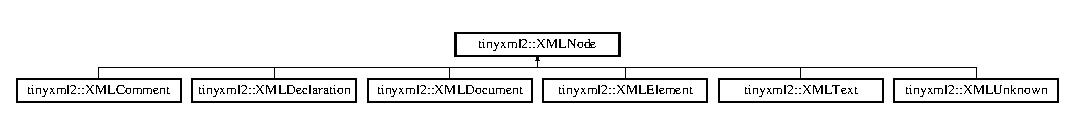
\includegraphics[height=1.145194cm]{classtinyxml2_1_1_x_m_l_node}
\end{center}
\end{figure}
\subsection*{Public Member Functions}
\begin{DoxyCompactItemize}
\item 
\mbox{\Hypertarget{classtinyxml2_1_1_x_m_l_node_a2de84cfa4ec3fe249bad745069d145f1}\label{classtinyxml2_1_1_x_m_l_node_a2de84cfa4ec3fe249bad745069d145f1}} 
const \mbox{\hyperlink{classtinyxml2_1_1_x_m_l_document}{X\+M\+L\+Document}} $\ast$ \mbox{\hyperlink{classtinyxml2_1_1_x_m_l_node_a2de84cfa4ec3fe249bad745069d145f1}{Get\+Document}} () const
\begin{DoxyCompactList}\small\item\em Get the \mbox{\hyperlink{classtinyxml2_1_1_x_m_l_document}{X\+M\+L\+Document}} that owns this \mbox{\hyperlink{classtinyxml2_1_1_x_m_l_node}{X\+M\+L\+Node}}. \end{DoxyCompactList}\item 
\mbox{\Hypertarget{classtinyxml2_1_1_x_m_l_node_af343d1ef0b45c0020e62d784d7e67a68}\label{classtinyxml2_1_1_x_m_l_node_af343d1ef0b45c0020e62d784d7e67a68}} 
\mbox{\hyperlink{classtinyxml2_1_1_x_m_l_document}{X\+M\+L\+Document}} $\ast$ \mbox{\hyperlink{classtinyxml2_1_1_x_m_l_node_af343d1ef0b45c0020e62d784d7e67a68}{Get\+Document}} ()
\begin{DoxyCompactList}\small\item\em Get the \mbox{\hyperlink{classtinyxml2_1_1_x_m_l_document}{X\+M\+L\+Document}} that owns this \mbox{\hyperlink{classtinyxml2_1_1_x_m_l_node}{X\+M\+L\+Node}}. \end{DoxyCompactList}\item 
\mbox{\Hypertarget{classtinyxml2_1_1_x_m_l_node_aab516e699567f75cc9ab2ef2eee501e8}\label{classtinyxml2_1_1_x_m_l_node_aab516e699567f75cc9ab2ef2eee501e8}} 
virtual \mbox{\hyperlink{classtinyxml2_1_1_x_m_l_element}{X\+M\+L\+Element}} $\ast$ \mbox{\hyperlink{classtinyxml2_1_1_x_m_l_node_aab516e699567f75cc9ab2ef2eee501e8}{To\+Element}} ()
\begin{DoxyCompactList}\small\item\em Safely cast to an Element, or null. \end{DoxyCompactList}\item 
\mbox{\Hypertarget{classtinyxml2_1_1_x_m_l_node_a41c55dab9162d1eb62db2008430e376b}\label{classtinyxml2_1_1_x_m_l_node_a41c55dab9162d1eb62db2008430e376b}} 
virtual \mbox{\hyperlink{classtinyxml2_1_1_x_m_l_text}{X\+M\+L\+Text}} $\ast$ \mbox{\hyperlink{classtinyxml2_1_1_x_m_l_node_a41c55dab9162d1eb62db2008430e376b}{To\+Text}} ()
\begin{DoxyCompactList}\small\item\em Safely cast to Text, or null. \end{DoxyCompactList}\item 
\mbox{\Hypertarget{classtinyxml2_1_1_x_m_l_node_aff47671055aa99840a1c1ebd661e63e3}\label{classtinyxml2_1_1_x_m_l_node_aff47671055aa99840a1c1ebd661e63e3}} 
virtual \mbox{\hyperlink{classtinyxml2_1_1_x_m_l_comment}{X\+M\+L\+Comment}} $\ast$ \mbox{\hyperlink{classtinyxml2_1_1_x_m_l_node_aff47671055aa99840a1c1ebd661e63e3}{To\+Comment}} ()
\begin{DoxyCompactList}\small\item\em Safely cast to a Comment, or null. \end{DoxyCompactList}\item 
\mbox{\Hypertarget{classtinyxml2_1_1_x_m_l_node_a836e2966ed736fc3c94f70e12a2a3357}\label{classtinyxml2_1_1_x_m_l_node_a836e2966ed736fc3c94f70e12a2a3357}} 
virtual \mbox{\hyperlink{classtinyxml2_1_1_x_m_l_document}{X\+M\+L\+Document}} $\ast$ \mbox{\hyperlink{classtinyxml2_1_1_x_m_l_node_a836e2966ed736fc3c94f70e12a2a3357}{To\+Document}} ()
\begin{DoxyCompactList}\small\item\em Safely cast to a Document, or null. \end{DoxyCompactList}\item 
\mbox{\Hypertarget{classtinyxml2_1_1_x_m_l_node_a174fd4c22c010b58138c1b84a0dfbd51}\label{classtinyxml2_1_1_x_m_l_node_a174fd4c22c010b58138c1b84a0dfbd51}} 
virtual \mbox{\hyperlink{classtinyxml2_1_1_x_m_l_declaration}{X\+M\+L\+Declaration}} $\ast$ \mbox{\hyperlink{classtinyxml2_1_1_x_m_l_node_a174fd4c22c010b58138c1b84a0dfbd51}{To\+Declaration}} ()
\begin{DoxyCompactList}\small\item\em Safely cast to a Declaration, or null. \end{DoxyCompactList}\item 
\mbox{\Hypertarget{classtinyxml2_1_1_x_m_l_node_a8675a74aa0ada6eccab0c77ef3e5b9bd}\label{classtinyxml2_1_1_x_m_l_node_a8675a74aa0ada6eccab0c77ef3e5b9bd}} 
virtual \mbox{\hyperlink{classtinyxml2_1_1_x_m_l_unknown}{X\+M\+L\+Unknown}} $\ast$ \mbox{\hyperlink{classtinyxml2_1_1_x_m_l_node_a8675a74aa0ada6eccab0c77ef3e5b9bd}{To\+Unknown}} ()
\begin{DoxyCompactList}\small\item\em Safely cast to an Unknown, or null. \end{DoxyCompactList}\item 
\mbox{\Hypertarget{classtinyxml2_1_1_x_m_l_node_a2c5c843b8f37306f15994ebe882b9346}\label{classtinyxml2_1_1_x_m_l_node_a2c5c843b8f37306f15994ebe882b9346}} 
virtual const \mbox{\hyperlink{classtinyxml2_1_1_x_m_l_element}{X\+M\+L\+Element}} $\ast$ {\bfseries To\+Element} () const
\item 
\mbox{\Hypertarget{classtinyxml2_1_1_x_m_l_node_acb9ccc1beda27c0efcb0545683c3e7f4}\label{classtinyxml2_1_1_x_m_l_node_acb9ccc1beda27c0efcb0545683c3e7f4}} 
virtual const \mbox{\hyperlink{classtinyxml2_1_1_x_m_l_text}{X\+M\+L\+Text}} $\ast$ {\bfseries To\+Text} () const
\item 
\mbox{\Hypertarget{classtinyxml2_1_1_x_m_l_node_a6a53bb83faf5c0ccc95b6cf74dba0025}\label{classtinyxml2_1_1_x_m_l_node_a6a53bb83faf5c0ccc95b6cf74dba0025}} 
virtual const \mbox{\hyperlink{classtinyxml2_1_1_x_m_l_comment}{X\+M\+L\+Comment}} $\ast$ {\bfseries To\+Comment} () const
\item 
\mbox{\Hypertarget{classtinyxml2_1_1_x_m_l_node_ae8a5250331a5f12e10843fcb5ef3ef0b}\label{classtinyxml2_1_1_x_m_l_node_ae8a5250331a5f12e10843fcb5ef3ef0b}} 
virtual const \mbox{\hyperlink{classtinyxml2_1_1_x_m_l_document}{X\+M\+L\+Document}} $\ast$ {\bfseries To\+Document} () const
\item 
\mbox{\Hypertarget{classtinyxml2_1_1_x_m_l_node_ac48bb4bf9eb7bb3654ad4b94945db9a1}\label{classtinyxml2_1_1_x_m_l_node_ac48bb4bf9eb7bb3654ad4b94945db9a1}} 
virtual const \mbox{\hyperlink{classtinyxml2_1_1_x_m_l_declaration}{X\+M\+L\+Declaration}} $\ast$ {\bfseries To\+Declaration} () const
\item 
\mbox{\Hypertarget{classtinyxml2_1_1_x_m_l_node_af29ffd6cbe609b6fa04a705256150408}\label{classtinyxml2_1_1_x_m_l_node_af29ffd6cbe609b6fa04a705256150408}} 
virtual const \mbox{\hyperlink{classtinyxml2_1_1_x_m_l_unknown}{X\+M\+L\+Unknown}} $\ast$ {\bfseries To\+Unknown} () const
\item 
const char $\ast$ \mbox{\hyperlink{classtinyxml2_1_1_x_m_l_node_a0485e51c670e741884cfd8362274d680}{Value}} () const
\item 
void \mbox{\hyperlink{classtinyxml2_1_1_x_m_l_node_a09dd68cf9eae137579f6e50f36487513}{Set\+Value}} (const char $\ast$val, bool static\+Mem=false)
\item 
\mbox{\Hypertarget{classtinyxml2_1_1_x_m_l_node_a9b5fc636646fda761d342c72e91cb286}\label{classtinyxml2_1_1_x_m_l_node_a9b5fc636646fda761d342c72e91cb286}} 
int \mbox{\hyperlink{classtinyxml2_1_1_x_m_l_node_a9b5fc636646fda761d342c72e91cb286}{Get\+Line\+Num}} () const
\begin{DoxyCompactList}\small\item\em Gets the line number the node is in, if the document was parsed from a file. \end{DoxyCompactList}\item 
\mbox{\Hypertarget{classtinyxml2_1_1_x_m_l_node_ae0f62bc186c56c2e0483ebd52dbfbe34}\label{classtinyxml2_1_1_x_m_l_node_ae0f62bc186c56c2e0483ebd52dbfbe34}} 
const \mbox{\hyperlink{classtinyxml2_1_1_x_m_l_node}{X\+M\+L\+Node}} $\ast$ \mbox{\hyperlink{classtinyxml2_1_1_x_m_l_node_ae0f62bc186c56c2e0483ebd52dbfbe34}{Parent}} () const
\begin{DoxyCompactList}\small\item\em Get the parent of this node on the D\+OM. \end{DoxyCompactList}\item 
\mbox{\Hypertarget{classtinyxml2_1_1_x_m_l_node_a76029693a5a54fbb721a41d7a0ca8a97}\label{classtinyxml2_1_1_x_m_l_node_a76029693a5a54fbb721a41d7a0ca8a97}} 
\mbox{\hyperlink{classtinyxml2_1_1_x_m_l_node}{X\+M\+L\+Node}} $\ast$ {\bfseries Parent} ()
\item 
\mbox{\Hypertarget{classtinyxml2_1_1_x_m_l_node_ac3ab489e6e202a3cd1762d3b332e89d4}\label{classtinyxml2_1_1_x_m_l_node_ac3ab489e6e202a3cd1762d3b332e89d4}} 
bool \mbox{\hyperlink{classtinyxml2_1_1_x_m_l_node_ac3ab489e6e202a3cd1762d3b332e89d4}{No\+Children}} () const
\begin{DoxyCompactList}\small\item\em Returns true if this node has no children. \end{DoxyCompactList}\item 
\mbox{\Hypertarget{classtinyxml2_1_1_x_m_l_node_ae7dc225e1018cdd685f7563593a1fe08}\label{classtinyxml2_1_1_x_m_l_node_ae7dc225e1018cdd685f7563593a1fe08}} 
const \mbox{\hyperlink{classtinyxml2_1_1_x_m_l_node}{X\+M\+L\+Node}} $\ast$ \mbox{\hyperlink{classtinyxml2_1_1_x_m_l_node_ae7dc225e1018cdd685f7563593a1fe08}{First\+Child}} () const
\begin{DoxyCompactList}\small\item\em Get the first child node, or null if none exists. \end{DoxyCompactList}\item 
\mbox{\Hypertarget{classtinyxml2_1_1_x_m_l_node_a2d6c70c475146b48bc93a7fafdeff5e0}\label{classtinyxml2_1_1_x_m_l_node_a2d6c70c475146b48bc93a7fafdeff5e0}} 
\mbox{\hyperlink{classtinyxml2_1_1_x_m_l_node}{X\+M\+L\+Node}} $\ast$ {\bfseries First\+Child} ()
\item 
const \mbox{\hyperlink{classtinyxml2_1_1_x_m_l_element}{X\+M\+L\+Element}} $\ast$ \mbox{\hyperlink{classtinyxml2_1_1_x_m_l_node_a1bec132dcf085284e0a10755f2cf0d57}{First\+Child\+Element}} (const char $\ast$name=0) const
\item 
\mbox{\Hypertarget{classtinyxml2_1_1_x_m_l_node_af1e0e475cc27d5e7eeaf4d732691b741}\label{classtinyxml2_1_1_x_m_l_node_af1e0e475cc27d5e7eeaf4d732691b741}} 
\mbox{\hyperlink{classtinyxml2_1_1_x_m_l_element}{X\+M\+L\+Element}} $\ast$ {\bfseries First\+Child\+Element} (const char $\ast$name=0)
\item 
\mbox{\Hypertarget{classtinyxml2_1_1_x_m_l_node_a9b8583a277e8e26f4cbbb5492786778e}\label{classtinyxml2_1_1_x_m_l_node_a9b8583a277e8e26f4cbbb5492786778e}} 
const \mbox{\hyperlink{classtinyxml2_1_1_x_m_l_node}{X\+M\+L\+Node}} $\ast$ \mbox{\hyperlink{classtinyxml2_1_1_x_m_l_node_a9b8583a277e8e26f4cbbb5492786778e}{Last\+Child}} () const
\begin{DoxyCompactList}\small\item\em Get the last child node, or null if none exists. \end{DoxyCompactList}\item 
\mbox{\Hypertarget{classtinyxml2_1_1_x_m_l_node_ad7552c8cb1dc0cb6f3bdc14a9d115dbf}\label{classtinyxml2_1_1_x_m_l_node_ad7552c8cb1dc0cb6f3bdc14a9d115dbf}} 
\mbox{\hyperlink{classtinyxml2_1_1_x_m_l_node}{X\+M\+L\+Node}} $\ast$ {\bfseries Last\+Child} ()
\item 
const \mbox{\hyperlink{classtinyxml2_1_1_x_m_l_element}{X\+M\+L\+Element}} $\ast$ \mbox{\hyperlink{classtinyxml2_1_1_x_m_l_node_a609e02f02044f39b928d1a3e0de9f532}{Last\+Child\+Element}} (const char $\ast$name=0) const
\item 
\mbox{\Hypertarget{classtinyxml2_1_1_x_m_l_node_a1b77a8194d059665a4412ebfea276878}\label{classtinyxml2_1_1_x_m_l_node_a1b77a8194d059665a4412ebfea276878}} 
\mbox{\hyperlink{classtinyxml2_1_1_x_m_l_element}{X\+M\+L\+Element}} $\ast$ {\bfseries Last\+Child\+Element} (const char $\ast$name=0)
\item 
\mbox{\Hypertarget{classtinyxml2_1_1_x_m_l_node_aac667c513d445f8b783e1e15ef9d3551}\label{classtinyxml2_1_1_x_m_l_node_aac667c513d445f8b783e1e15ef9d3551}} 
const \mbox{\hyperlink{classtinyxml2_1_1_x_m_l_node}{X\+M\+L\+Node}} $\ast$ \mbox{\hyperlink{classtinyxml2_1_1_x_m_l_node_aac667c513d445f8b783e1e15ef9d3551}{Previous\+Sibling}} () const
\begin{DoxyCompactList}\small\item\em Get the previous (left) sibling node of this node. \end{DoxyCompactList}\item 
\mbox{\Hypertarget{classtinyxml2_1_1_x_m_l_node_ae760e5e7e766df1d2cf3bb4a847876d6}\label{classtinyxml2_1_1_x_m_l_node_ae760e5e7e766df1d2cf3bb4a847876d6}} 
\mbox{\hyperlink{classtinyxml2_1_1_x_m_l_node}{X\+M\+L\+Node}} $\ast$ {\bfseries Previous\+Sibling} ()
\item 
\mbox{\Hypertarget{classtinyxml2_1_1_x_m_l_node_a9453cda5e970375a7b1b2099f8a7c40a}\label{classtinyxml2_1_1_x_m_l_node_a9453cda5e970375a7b1b2099f8a7c40a}} 
const \mbox{\hyperlink{classtinyxml2_1_1_x_m_l_element}{X\+M\+L\+Element}} $\ast$ \mbox{\hyperlink{classtinyxml2_1_1_x_m_l_node_a9453cda5e970375a7b1b2099f8a7c40a}{Previous\+Sibling\+Element}} (const char $\ast$name=0) const
\begin{DoxyCompactList}\small\item\em Get the previous (left) sibling element of this node, with an optionally supplied name. \end{DoxyCompactList}\item 
\mbox{\Hypertarget{classtinyxml2_1_1_x_m_l_node_ae4f37eb6cd405bdf1d57caa066e36d87}\label{classtinyxml2_1_1_x_m_l_node_ae4f37eb6cd405bdf1d57caa066e36d87}} 
\mbox{\hyperlink{classtinyxml2_1_1_x_m_l_element}{X\+M\+L\+Element}} $\ast$ {\bfseries Previous\+Sibling\+Element} (const char $\ast$name=0)
\item 
\mbox{\Hypertarget{classtinyxml2_1_1_x_m_l_node_a79db9ef0fe014d27790f2218b87bcbb5}\label{classtinyxml2_1_1_x_m_l_node_a79db9ef0fe014d27790f2218b87bcbb5}} 
const \mbox{\hyperlink{classtinyxml2_1_1_x_m_l_node}{X\+M\+L\+Node}} $\ast$ \mbox{\hyperlink{classtinyxml2_1_1_x_m_l_node_a79db9ef0fe014d27790f2218b87bcbb5}{Next\+Sibling}} () const
\begin{DoxyCompactList}\small\item\em Get the next (right) sibling node of this node. \end{DoxyCompactList}\item 
\mbox{\Hypertarget{classtinyxml2_1_1_x_m_l_node_aeb7d4dfd8fb924ef86e7cb72183acbac}\label{classtinyxml2_1_1_x_m_l_node_aeb7d4dfd8fb924ef86e7cb72183acbac}} 
\mbox{\hyperlink{classtinyxml2_1_1_x_m_l_node}{X\+M\+L\+Node}} $\ast$ {\bfseries Next\+Sibling} ()
\item 
\mbox{\Hypertarget{classtinyxml2_1_1_x_m_l_node_a14ea560df31110ff07a9f566171bf797}\label{classtinyxml2_1_1_x_m_l_node_a14ea560df31110ff07a9f566171bf797}} 
const \mbox{\hyperlink{classtinyxml2_1_1_x_m_l_element}{X\+M\+L\+Element}} $\ast$ \mbox{\hyperlink{classtinyxml2_1_1_x_m_l_node_a14ea560df31110ff07a9f566171bf797}{Next\+Sibling\+Element}} (const char $\ast$name=0) const
\begin{DoxyCompactList}\small\item\em Get the next (right) sibling element of this node, with an optionally supplied name. \end{DoxyCompactList}\item 
\mbox{\Hypertarget{classtinyxml2_1_1_x_m_l_node_af1225412584d4a2126f55e96a12e0ec0}\label{classtinyxml2_1_1_x_m_l_node_af1225412584d4a2126f55e96a12e0ec0}} 
\mbox{\hyperlink{classtinyxml2_1_1_x_m_l_element}{X\+M\+L\+Element}} $\ast$ {\bfseries Next\+Sibling\+Element} (const char $\ast$name=0)
\item 
\mbox{\hyperlink{classtinyxml2_1_1_x_m_l_node}{X\+M\+L\+Node}} $\ast$ \mbox{\hyperlink{classtinyxml2_1_1_x_m_l_node_ae3b422e98914d6002ca99bb1d2837103}{Insert\+End\+Child}} (\mbox{\hyperlink{classtinyxml2_1_1_x_m_l_node}{X\+M\+L\+Node}} $\ast$add\+This)
\item 
\mbox{\Hypertarget{classtinyxml2_1_1_x_m_l_node_a663e3a5a378169fd477378f4d17a7649}\label{classtinyxml2_1_1_x_m_l_node_a663e3a5a378169fd477378f4d17a7649}} 
\mbox{\hyperlink{classtinyxml2_1_1_x_m_l_node}{X\+M\+L\+Node}} $\ast$ {\bfseries Link\+End\+Child} (\mbox{\hyperlink{classtinyxml2_1_1_x_m_l_node}{X\+M\+L\+Node}} $\ast$add\+This)
\item 
\mbox{\hyperlink{classtinyxml2_1_1_x_m_l_node}{X\+M\+L\+Node}} $\ast$ \mbox{\hyperlink{classtinyxml2_1_1_x_m_l_node_ac609a8f3ea949027f439280c640bbaf2}{Insert\+First\+Child}} (\mbox{\hyperlink{classtinyxml2_1_1_x_m_l_node}{X\+M\+L\+Node}} $\ast$add\+This)
\item 
\mbox{\hyperlink{classtinyxml2_1_1_x_m_l_node}{X\+M\+L\+Node}} $\ast$ \mbox{\hyperlink{classtinyxml2_1_1_x_m_l_node_a9275138a1b8dd5d8e2c26789bdc23ac8}{Insert\+After\+Child}} (\mbox{\hyperlink{classtinyxml2_1_1_x_m_l_node}{X\+M\+L\+Node}} $\ast$after\+This, \mbox{\hyperlink{classtinyxml2_1_1_x_m_l_node}{X\+M\+L\+Node}} $\ast$add\+This)
\item 
void \mbox{\hyperlink{classtinyxml2_1_1_x_m_l_node_a0360085cc54df5bff85d5c5da13afdce}{Delete\+Children}} ()
\item 
void \mbox{\hyperlink{classtinyxml2_1_1_x_m_l_node_a363b6edbd6ebd55f8387d2b89f2b0921}{Delete\+Child}} (\mbox{\hyperlink{classtinyxml2_1_1_x_m_l_node}{X\+M\+L\+Node}} $\ast$node)
\item 
virtual \mbox{\hyperlink{classtinyxml2_1_1_x_m_l_node}{X\+M\+L\+Node}} $\ast$ \mbox{\hyperlink{classtinyxml2_1_1_x_m_l_node_a8402cbd3129d20e9e6024bbcc0531283}{Shallow\+Clone}} (\mbox{\hyperlink{classtinyxml2_1_1_x_m_l_document}{X\+M\+L\+Document}} $\ast$document) const =0
\item 
\mbox{\hyperlink{classtinyxml2_1_1_x_m_l_node}{X\+M\+L\+Node}} $\ast$ \mbox{\hyperlink{classtinyxml2_1_1_x_m_l_node_a3bb369fd733f1989b751d99a9417adab}{Deep\+Clone}} (\mbox{\hyperlink{classtinyxml2_1_1_x_m_l_document}{X\+M\+L\+Document}} $\ast$target) const
\item 
virtual bool \mbox{\hyperlink{classtinyxml2_1_1_x_m_l_node_a7ce18b751c3ea09eac292dca264f9226}{Shallow\+Equal}} (const \mbox{\hyperlink{classtinyxml2_1_1_x_m_l_node}{X\+M\+L\+Node}} $\ast$compare) const =0
\item 
virtual bool \mbox{\hyperlink{classtinyxml2_1_1_x_m_l_node_a81e66df0a44c67a7af17f3b77a152785}{Accept}} (\mbox{\hyperlink{classtinyxml2_1_1_x_m_l_visitor}{X\+M\+L\+Visitor}} $\ast$visitor) const =0
\item 
void \mbox{\hyperlink{classtinyxml2_1_1_x_m_l_node_a002978fc889cc011d143185f2377eca2}{Set\+User\+Data}} (void $\ast$user\+Data)
\item 
void $\ast$ \mbox{\hyperlink{classtinyxml2_1_1_x_m_l_node_a7f0687574afa03bc479dc44f29db0afe}{Get\+User\+Data}} () const
\end{DoxyCompactItemize}
\subsection*{Protected Member Functions}
\begin{DoxyCompactItemize}
\item 
\mbox{\Hypertarget{classtinyxml2_1_1_x_m_l_node_a29868df6ca383d574f584dfdd15105b6}\label{classtinyxml2_1_1_x_m_l_node_a29868df6ca383d574f584dfdd15105b6}} 
{\bfseries X\+M\+L\+Node} (\mbox{\hyperlink{classtinyxml2_1_1_x_m_l_document}{X\+M\+L\+Document}} $\ast$)
\item 
\mbox{\Hypertarget{classtinyxml2_1_1_x_m_l_node_a916e498914baecbc9a1f012352ef7c69}\label{classtinyxml2_1_1_x_m_l_node_a916e498914baecbc9a1f012352ef7c69}} 
virtual char $\ast$ {\bfseries Parse\+Deep} (char $\ast$p, \mbox{\hyperlink{classtinyxml2_1_1_str_pair}{Str\+Pair}} $\ast$parent\+End\+Tag, int $\ast$cur\+Line\+Num\+Ptr)
\end{DoxyCompactItemize}
\subsection*{Protected Attributes}
\begin{DoxyCompactItemize}
\item 
\mbox{\Hypertarget{classtinyxml2_1_1_x_m_l_node_a8d2d2be0bb6797625551eb0e91f0ff62}\label{classtinyxml2_1_1_x_m_l_node_a8d2d2be0bb6797625551eb0e91f0ff62}} 
\mbox{\hyperlink{classtinyxml2_1_1_x_m_l_document}{X\+M\+L\+Document}} $\ast$ {\bfseries \+\_\+document}
\item 
\mbox{\Hypertarget{classtinyxml2_1_1_x_m_l_node_a176dd1c4965c21c366de192164aa2c13}\label{classtinyxml2_1_1_x_m_l_node_a176dd1c4965c21c366de192164aa2c13}} 
\mbox{\hyperlink{classtinyxml2_1_1_x_m_l_node}{X\+M\+L\+Node}} $\ast$ {\bfseries \+\_\+parent}
\item 
\mbox{\Hypertarget{classtinyxml2_1_1_x_m_l_node_a3ea9884098b8379de2bb5ab3fc85c0fc}\label{classtinyxml2_1_1_x_m_l_node_a3ea9884098b8379de2bb5ab3fc85c0fc}} 
\mbox{\hyperlink{classtinyxml2_1_1_str_pair}{Str\+Pair}} {\bfseries \+\_\+value}
\item 
\mbox{\Hypertarget{classtinyxml2_1_1_x_m_l_node_ab336ed023e15be202ff3b410be01b804}\label{classtinyxml2_1_1_x_m_l_node_ab336ed023e15be202ff3b410be01b804}} 
int {\bfseries \+\_\+parse\+Line\+Num}
\item 
\mbox{\Hypertarget{classtinyxml2_1_1_x_m_l_node_aa20c91e4213dc930c5bdf420322ca342}\label{classtinyxml2_1_1_x_m_l_node_aa20c91e4213dc930c5bdf420322ca342}} 
\mbox{\hyperlink{classtinyxml2_1_1_x_m_l_node}{X\+M\+L\+Node}} $\ast$ {\bfseries \+\_\+first\+Child}
\item 
\mbox{\Hypertarget{classtinyxml2_1_1_x_m_l_node_a099b6560ae44ab9edb8453aaf1a3747b}\label{classtinyxml2_1_1_x_m_l_node_a099b6560ae44ab9edb8453aaf1a3747b}} 
\mbox{\hyperlink{classtinyxml2_1_1_x_m_l_node}{X\+M\+L\+Node}} $\ast$ {\bfseries \+\_\+last\+Child}
\item 
\mbox{\Hypertarget{classtinyxml2_1_1_x_m_l_node_a9739eb0fb9a1188266052055e7a6bf6b}\label{classtinyxml2_1_1_x_m_l_node_a9739eb0fb9a1188266052055e7a6bf6b}} 
\mbox{\hyperlink{classtinyxml2_1_1_x_m_l_node}{X\+M\+L\+Node}} $\ast$ {\bfseries \+\_\+prev}
\item 
\mbox{\Hypertarget{classtinyxml2_1_1_x_m_l_node_a27e985496b37dd00eb5b9cf59b9e3fb1}\label{classtinyxml2_1_1_x_m_l_node_a27e985496b37dd00eb5b9cf59b9e3fb1}} 
\mbox{\hyperlink{classtinyxml2_1_1_x_m_l_node}{X\+M\+L\+Node}} $\ast$ {\bfseries \+\_\+next}
\item 
\mbox{\Hypertarget{classtinyxml2_1_1_x_m_l_node_ac2d5cc463a6c95ec5907d57a119c56da}\label{classtinyxml2_1_1_x_m_l_node_ac2d5cc463a6c95ec5907d57a119c56da}} 
void $\ast$ {\bfseries \+\_\+user\+Data}
\end{DoxyCompactItemize}
\subsection*{Friends}
\begin{DoxyCompactItemize}
\item 
\mbox{\Hypertarget{classtinyxml2_1_1_x_m_l_node_a4eee3bda60c60a30e4e8cd4ea91c4c6e}\label{classtinyxml2_1_1_x_m_l_node_a4eee3bda60c60a30e4e8cd4ea91c4c6e}} 
class {\bfseries X\+M\+L\+Document}
\item 
\mbox{\Hypertarget{classtinyxml2_1_1_x_m_l_node_ac2fba9b6e452829dd892f7392c24e0eb}\label{classtinyxml2_1_1_x_m_l_node_ac2fba9b6e452829dd892f7392c24e0eb}} 
class {\bfseries X\+M\+L\+Element}
\end{DoxyCompactItemize}


\subsection{Detailed Description}
\mbox{\hyperlink{classtinyxml2_1_1_x_m_l_node}{X\+M\+L\+Node}} is a base class for every object that is in the X\+ML Document Object Model (D\+OM), except X\+M\+L\+Attributes. Nodes have siblings, a parent, and children which can be navigated. A node is always in a \mbox{\hyperlink{classtinyxml2_1_1_x_m_l_document}{X\+M\+L\+Document}}. The type of a \mbox{\hyperlink{classtinyxml2_1_1_x_m_l_node}{X\+M\+L\+Node}} can be queried, and it can be cast to its more defined type.

A \mbox{\hyperlink{classtinyxml2_1_1_x_m_l_document}{X\+M\+L\+Document}} allocates memory for all its Nodes. When the \mbox{\hyperlink{classtinyxml2_1_1_x_m_l_document}{X\+M\+L\+Document}} gets deleted, all its Nodes will also be deleted.

\begin{DoxyVerb}A Document can contain: Element (container or leaf)
                        Comment (leaf)
                        Unknown (leaf)
                        Declaration( leaf )

An Element can contain: Element (container or leaf)
                        Text    (leaf)
                        Attributes (not on tree)
                        Comment (leaf)
                        Unknown (leaf)\end{DoxyVerb}
 

\subsection{Member Function Documentation}
\mbox{\Hypertarget{classtinyxml2_1_1_x_m_l_node_a81e66df0a44c67a7af17f3b77a152785}\label{classtinyxml2_1_1_x_m_l_node_a81e66df0a44c67a7af17f3b77a152785}} 
\index{tinyxml2\+::\+X\+M\+L\+Node@{tinyxml2\+::\+X\+M\+L\+Node}!Accept@{Accept}}
\index{Accept@{Accept}!tinyxml2\+::\+X\+M\+L\+Node@{tinyxml2\+::\+X\+M\+L\+Node}}
\subsubsection{\texorpdfstring{Accept()}{Accept()}}
{\footnotesize\ttfamily virtual bool tinyxml2\+::\+X\+M\+L\+Node\+::\+Accept (\begin{DoxyParamCaption}\item[{\mbox{\hyperlink{classtinyxml2_1_1_x_m_l_visitor}{X\+M\+L\+Visitor}} $\ast$}]{visitor }\end{DoxyParamCaption}) const\hspace{0.3cm}{\ttfamily [pure virtual]}}

Accept a hierarchical visit of the nodes in the Tiny\+X\+M\+L-\/2 D\+OM. Every node in the X\+ML tree will be conditionally visited and the host will be called back via the \mbox{\hyperlink{classtinyxml2_1_1_x_m_l_visitor}{X\+M\+L\+Visitor}} interface.

This is essentially a S\+AX interface for Tiny\+X\+M\+L-\/2. (Note however it doesn\textquotesingle{}t re-\/parse the X\+ML for the callbacks, so the performance of Tiny\+X\+M\+L-\/2 is unchanged by using this interface versus any other.)

The interface has been based on ideas from\+:


\begin{DoxyItemize}
\item \href{http://www.saxproject.org/}{\tt http\+://www.\+saxproject.\+org/}
\item \href{http://c2.com/cgi/wiki?HierarchicalVisitorPattern}{\tt http\+://c2.\+com/cgi/wiki?\+Hierarchical\+Visitor\+Pattern}
\end{DoxyItemize}

Which are both good references for \char`\"{}visiting\char`\"{}.

An example of using \mbox{\hyperlink{classtinyxml2_1_1_x_m_l_node_a81e66df0a44c67a7af17f3b77a152785}{Accept()}}\+: \begin{DoxyVerb}XMLPrinter printer;
tinyxmlDoc.Accept( &printer );
const char* xmlcstr = printer.CStr();
\end{DoxyVerb}
 

Implemented in \mbox{\hyperlink{classtinyxml2_1_1_x_m_l_document_ab7be651917a35ab1ff0e4e6d4e565cdf}{tinyxml2\+::\+X\+M\+L\+Document}}, \mbox{\hyperlink{classtinyxml2_1_1_x_m_l_element_a9b2119831e8b85827d5d3e5076788e4a}{tinyxml2\+::\+X\+M\+L\+Element}}, \mbox{\hyperlink{classtinyxml2_1_1_x_m_l_unknown_a8a06b8c82117ca969a432e17a46830fc}{tinyxml2\+::\+X\+M\+L\+Unknown}}, \mbox{\hyperlink{classtinyxml2_1_1_x_m_l_declaration_acf47629d9fc08ed6f1c164a97bcf794b}{tinyxml2\+::\+X\+M\+L\+Declaration}}, \mbox{\hyperlink{classtinyxml2_1_1_x_m_l_comment_a27b37d16cea01b5329dfbbb4f9508e39}{tinyxml2\+::\+X\+M\+L\+Comment}}, and \mbox{\hyperlink{classtinyxml2_1_1_x_m_l_text_a537c60d7e18fb59c45ac2737a29ac47a}{tinyxml2\+::\+X\+M\+L\+Text}}.

\mbox{\Hypertarget{classtinyxml2_1_1_x_m_l_node_a3bb369fd733f1989b751d99a9417adab}\label{classtinyxml2_1_1_x_m_l_node_a3bb369fd733f1989b751d99a9417adab}} 
\index{tinyxml2\+::\+X\+M\+L\+Node@{tinyxml2\+::\+X\+M\+L\+Node}!Deep\+Clone@{Deep\+Clone}}
\index{Deep\+Clone@{Deep\+Clone}!tinyxml2\+::\+X\+M\+L\+Node@{tinyxml2\+::\+X\+M\+L\+Node}}
\subsubsection{\texorpdfstring{Deep\+Clone()}{DeepClone()}}
{\footnotesize\ttfamily \mbox{\hyperlink{classtinyxml2_1_1_x_m_l_node}{X\+M\+L\+Node}} $\ast$ tinyxml2\+::\+X\+M\+L\+Node\+::\+Deep\+Clone (\begin{DoxyParamCaption}\item[{\mbox{\hyperlink{classtinyxml2_1_1_x_m_l_document}{X\+M\+L\+Document}} $\ast$}]{target }\end{DoxyParamCaption}) const}

Make a copy of this node and all its children.

If the \textquotesingle{}target\textquotesingle{} is null, then the nodes will be allocated in the current document. If \textquotesingle{}target\textquotesingle{} is specified, the memory will be allocated is the specified \mbox{\hyperlink{classtinyxml2_1_1_x_m_l_document}{X\+M\+L\+Document}}.

N\+O\+TE\+: This is probably not the correct tool to copy a document, since X\+M\+L\+Documents can have multiple top level X\+M\+L\+Nodes. You probably want to use \mbox{\hyperlink{classtinyxml2_1_1_x_m_l_document_af592ffc91514e25a39664521ac83db45}{X\+M\+L\+Document\+::\+Deep\+Copy()}} \mbox{\Hypertarget{classtinyxml2_1_1_x_m_l_node_a363b6edbd6ebd55f8387d2b89f2b0921}\label{classtinyxml2_1_1_x_m_l_node_a363b6edbd6ebd55f8387d2b89f2b0921}} 
\index{tinyxml2\+::\+X\+M\+L\+Node@{tinyxml2\+::\+X\+M\+L\+Node}!Delete\+Child@{Delete\+Child}}
\index{Delete\+Child@{Delete\+Child}!tinyxml2\+::\+X\+M\+L\+Node@{tinyxml2\+::\+X\+M\+L\+Node}}
\subsubsection{\texorpdfstring{Delete\+Child()}{DeleteChild()}}
{\footnotesize\ttfamily void tinyxml2\+::\+X\+M\+L\+Node\+::\+Delete\+Child (\begin{DoxyParamCaption}\item[{\mbox{\hyperlink{classtinyxml2_1_1_x_m_l_node}{X\+M\+L\+Node}} $\ast$}]{node }\end{DoxyParamCaption})}

Delete a child of this node. \mbox{\Hypertarget{classtinyxml2_1_1_x_m_l_node_a0360085cc54df5bff85d5c5da13afdce}\label{classtinyxml2_1_1_x_m_l_node_a0360085cc54df5bff85d5c5da13afdce}} 
\index{tinyxml2\+::\+X\+M\+L\+Node@{tinyxml2\+::\+X\+M\+L\+Node}!Delete\+Children@{Delete\+Children}}
\index{Delete\+Children@{Delete\+Children}!tinyxml2\+::\+X\+M\+L\+Node@{tinyxml2\+::\+X\+M\+L\+Node}}
\subsubsection{\texorpdfstring{Delete\+Children()}{DeleteChildren()}}
{\footnotesize\ttfamily void tinyxml2\+::\+X\+M\+L\+Node\+::\+Delete\+Children (\begin{DoxyParamCaption}{ }\end{DoxyParamCaption})}

Delete all the children of this node. \mbox{\Hypertarget{classtinyxml2_1_1_x_m_l_node_a1bec132dcf085284e0a10755f2cf0d57}\label{classtinyxml2_1_1_x_m_l_node_a1bec132dcf085284e0a10755f2cf0d57}} 
\index{tinyxml2\+::\+X\+M\+L\+Node@{tinyxml2\+::\+X\+M\+L\+Node}!First\+Child\+Element@{First\+Child\+Element}}
\index{First\+Child\+Element@{First\+Child\+Element}!tinyxml2\+::\+X\+M\+L\+Node@{tinyxml2\+::\+X\+M\+L\+Node}}
\subsubsection{\texorpdfstring{First\+Child\+Element()}{FirstChildElement()}}
{\footnotesize\ttfamily const \mbox{\hyperlink{classtinyxml2_1_1_x_m_l_element}{X\+M\+L\+Element}} $\ast$ tinyxml2\+::\+X\+M\+L\+Node\+::\+First\+Child\+Element (\begin{DoxyParamCaption}\item[{const char $\ast$}]{name = {\ttfamily 0} }\end{DoxyParamCaption}) const}

Get the first child element, or optionally the first child element with the specified name. \mbox{\Hypertarget{classtinyxml2_1_1_x_m_l_node_a7f0687574afa03bc479dc44f29db0afe}\label{classtinyxml2_1_1_x_m_l_node_a7f0687574afa03bc479dc44f29db0afe}} 
\index{tinyxml2\+::\+X\+M\+L\+Node@{tinyxml2\+::\+X\+M\+L\+Node}!Get\+User\+Data@{Get\+User\+Data}}
\index{Get\+User\+Data@{Get\+User\+Data}!tinyxml2\+::\+X\+M\+L\+Node@{tinyxml2\+::\+X\+M\+L\+Node}}
\subsubsection{\texorpdfstring{Get\+User\+Data()}{GetUserData()}}
{\footnotesize\ttfamily void$\ast$ tinyxml2\+::\+X\+M\+L\+Node\+::\+Get\+User\+Data (\begin{DoxyParamCaption}{ }\end{DoxyParamCaption}) const\hspace{0.3cm}{\ttfamily [inline]}}

Get user data set into the \mbox{\hyperlink{classtinyxml2_1_1_x_m_l_node}{X\+M\+L\+Node}}. Tiny\+X\+M\+L-\/2 in no way processes or interprets user data. It is initially 0. \mbox{\Hypertarget{classtinyxml2_1_1_x_m_l_node_a9275138a1b8dd5d8e2c26789bdc23ac8}\label{classtinyxml2_1_1_x_m_l_node_a9275138a1b8dd5d8e2c26789bdc23ac8}} 
\index{tinyxml2\+::\+X\+M\+L\+Node@{tinyxml2\+::\+X\+M\+L\+Node}!Insert\+After\+Child@{Insert\+After\+Child}}
\index{Insert\+After\+Child@{Insert\+After\+Child}!tinyxml2\+::\+X\+M\+L\+Node@{tinyxml2\+::\+X\+M\+L\+Node}}
\subsubsection{\texorpdfstring{Insert\+After\+Child()}{InsertAfterChild()}}
{\footnotesize\ttfamily \mbox{\hyperlink{classtinyxml2_1_1_x_m_l_node}{X\+M\+L\+Node}} $\ast$ tinyxml2\+::\+X\+M\+L\+Node\+::\+Insert\+After\+Child (\begin{DoxyParamCaption}\item[{\mbox{\hyperlink{classtinyxml2_1_1_x_m_l_node}{X\+M\+L\+Node}} $\ast$}]{after\+This,  }\item[{\mbox{\hyperlink{classtinyxml2_1_1_x_m_l_node}{X\+M\+L\+Node}} $\ast$}]{add\+This }\end{DoxyParamCaption})}

Add a node after the specified child node. If the child node is already part of the document, it is moved from its old location to the new location. Returns the add\+This argument or 0 if the after\+This node is not a child of this node, or if the node does not belong to the same document. \mbox{\Hypertarget{classtinyxml2_1_1_x_m_l_node_ae3b422e98914d6002ca99bb1d2837103}\label{classtinyxml2_1_1_x_m_l_node_ae3b422e98914d6002ca99bb1d2837103}} 
\index{tinyxml2\+::\+X\+M\+L\+Node@{tinyxml2\+::\+X\+M\+L\+Node}!Insert\+End\+Child@{Insert\+End\+Child}}
\index{Insert\+End\+Child@{Insert\+End\+Child}!tinyxml2\+::\+X\+M\+L\+Node@{tinyxml2\+::\+X\+M\+L\+Node}}
\subsubsection{\texorpdfstring{Insert\+End\+Child()}{InsertEndChild()}}
{\footnotesize\ttfamily \mbox{\hyperlink{classtinyxml2_1_1_x_m_l_node}{X\+M\+L\+Node}} $\ast$ tinyxml2\+::\+X\+M\+L\+Node\+::\+Insert\+End\+Child (\begin{DoxyParamCaption}\item[{\mbox{\hyperlink{classtinyxml2_1_1_x_m_l_node}{X\+M\+L\+Node}} $\ast$}]{add\+This }\end{DoxyParamCaption})}

Add a child node as the last (right) child. If the child node is already part of the document, it is moved from its old location to the new location. Returns the add\+This argument or 0 if the node does not belong to the same document. \mbox{\Hypertarget{classtinyxml2_1_1_x_m_l_node_ac609a8f3ea949027f439280c640bbaf2}\label{classtinyxml2_1_1_x_m_l_node_ac609a8f3ea949027f439280c640bbaf2}} 
\index{tinyxml2\+::\+X\+M\+L\+Node@{tinyxml2\+::\+X\+M\+L\+Node}!Insert\+First\+Child@{Insert\+First\+Child}}
\index{Insert\+First\+Child@{Insert\+First\+Child}!tinyxml2\+::\+X\+M\+L\+Node@{tinyxml2\+::\+X\+M\+L\+Node}}
\subsubsection{\texorpdfstring{Insert\+First\+Child()}{InsertFirstChild()}}
{\footnotesize\ttfamily \mbox{\hyperlink{classtinyxml2_1_1_x_m_l_node}{X\+M\+L\+Node}} $\ast$ tinyxml2\+::\+X\+M\+L\+Node\+::\+Insert\+First\+Child (\begin{DoxyParamCaption}\item[{\mbox{\hyperlink{classtinyxml2_1_1_x_m_l_node}{X\+M\+L\+Node}} $\ast$}]{add\+This }\end{DoxyParamCaption})}

Add a child node as the first (left) child. If the child node is already part of the document, it is moved from its old location to the new location. Returns the add\+This argument or 0 if the node does not belong to the same document. \mbox{\Hypertarget{classtinyxml2_1_1_x_m_l_node_a609e02f02044f39b928d1a3e0de9f532}\label{classtinyxml2_1_1_x_m_l_node_a609e02f02044f39b928d1a3e0de9f532}} 
\index{tinyxml2\+::\+X\+M\+L\+Node@{tinyxml2\+::\+X\+M\+L\+Node}!Last\+Child\+Element@{Last\+Child\+Element}}
\index{Last\+Child\+Element@{Last\+Child\+Element}!tinyxml2\+::\+X\+M\+L\+Node@{tinyxml2\+::\+X\+M\+L\+Node}}
\subsubsection{\texorpdfstring{Last\+Child\+Element()}{LastChildElement()}}
{\footnotesize\ttfamily const \mbox{\hyperlink{classtinyxml2_1_1_x_m_l_element}{X\+M\+L\+Element}} $\ast$ tinyxml2\+::\+X\+M\+L\+Node\+::\+Last\+Child\+Element (\begin{DoxyParamCaption}\item[{const char $\ast$}]{name = {\ttfamily 0} }\end{DoxyParamCaption}) const}

Get the last child element or optionally the last child element with the specified name. \mbox{\Hypertarget{classtinyxml2_1_1_x_m_l_node_a002978fc889cc011d143185f2377eca2}\label{classtinyxml2_1_1_x_m_l_node_a002978fc889cc011d143185f2377eca2}} 
\index{tinyxml2\+::\+X\+M\+L\+Node@{tinyxml2\+::\+X\+M\+L\+Node}!Set\+User\+Data@{Set\+User\+Data}}
\index{Set\+User\+Data@{Set\+User\+Data}!tinyxml2\+::\+X\+M\+L\+Node@{tinyxml2\+::\+X\+M\+L\+Node}}
\subsubsection{\texorpdfstring{Set\+User\+Data()}{SetUserData()}}
{\footnotesize\ttfamily void tinyxml2\+::\+X\+M\+L\+Node\+::\+Set\+User\+Data (\begin{DoxyParamCaption}\item[{void $\ast$}]{user\+Data }\end{DoxyParamCaption})\hspace{0.3cm}{\ttfamily [inline]}}

Set user data into the \mbox{\hyperlink{classtinyxml2_1_1_x_m_l_node}{X\+M\+L\+Node}}. Tiny\+X\+M\+L-\/2 in no way processes or interprets user data. It is initially 0. \mbox{\Hypertarget{classtinyxml2_1_1_x_m_l_node_a09dd68cf9eae137579f6e50f36487513}\label{classtinyxml2_1_1_x_m_l_node_a09dd68cf9eae137579f6e50f36487513}} 
\index{tinyxml2\+::\+X\+M\+L\+Node@{tinyxml2\+::\+X\+M\+L\+Node}!Set\+Value@{Set\+Value}}
\index{Set\+Value@{Set\+Value}!tinyxml2\+::\+X\+M\+L\+Node@{tinyxml2\+::\+X\+M\+L\+Node}}
\subsubsection{\texorpdfstring{Set\+Value()}{SetValue()}}
{\footnotesize\ttfamily void tinyxml2\+::\+X\+M\+L\+Node\+::\+Set\+Value (\begin{DoxyParamCaption}\item[{const char $\ast$}]{val,  }\item[{bool}]{static\+Mem = {\ttfamily false} }\end{DoxyParamCaption})}

Set the Value of an X\+ML node. \begin{DoxySeeAlso}{See also}
\mbox{\hyperlink{classtinyxml2_1_1_x_m_l_node_a0485e51c670e741884cfd8362274d680}{Value()}} 
\end{DoxySeeAlso}
\mbox{\Hypertarget{classtinyxml2_1_1_x_m_l_node_a8402cbd3129d20e9e6024bbcc0531283}\label{classtinyxml2_1_1_x_m_l_node_a8402cbd3129d20e9e6024bbcc0531283}} 
\index{tinyxml2\+::\+X\+M\+L\+Node@{tinyxml2\+::\+X\+M\+L\+Node}!Shallow\+Clone@{Shallow\+Clone}}
\index{Shallow\+Clone@{Shallow\+Clone}!tinyxml2\+::\+X\+M\+L\+Node@{tinyxml2\+::\+X\+M\+L\+Node}}
\subsubsection{\texorpdfstring{Shallow\+Clone()}{ShallowClone()}}
{\footnotesize\ttfamily virtual \mbox{\hyperlink{classtinyxml2_1_1_x_m_l_node}{X\+M\+L\+Node}}$\ast$ tinyxml2\+::\+X\+M\+L\+Node\+::\+Shallow\+Clone (\begin{DoxyParamCaption}\item[{\mbox{\hyperlink{classtinyxml2_1_1_x_m_l_document}{X\+M\+L\+Document}} $\ast$}]{document }\end{DoxyParamCaption}) const\hspace{0.3cm}{\ttfamily [pure virtual]}}

Make a copy of this node, but not its children. You may pass in a Document pointer that will be the owner of the new Node. If the \textquotesingle{}document\textquotesingle{} is null, then the node returned will be allocated from the current Document. (this-\/$>$\mbox{\hyperlink{classtinyxml2_1_1_x_m_l_node_af343d1ef0b45c0020e62d784d7e67a68}{Get\+Document()}})

Note\+: if called on a \mbox{\hyperlink{classtinyxml2_1_1_x_m_l_document}{X\+M\+L\+Document}}, this will return null. 

Implemented in \mbox{\hyperlink{classtinyxml2_1_1_x_m_l_document_aa37cc1709d7e1e988bc17dcfb24a69b8}{tinyxml2\+::\+X\+M\+L\+Document}}, \mbox{\hyperlink{classtinyxml2_1_1_x_m_l_element_aafa2807a45b28fe096b29d76e6a13b7c}{tinyxml2\+::\+X\+M\+L\+Element}}, \mbox{\hyperlink{classtinyxml2_1_1_x_m_l_unknown_ab73b48b819aa4b2ef3815dc2d7d20d5f}{tinyxml2\+::\+X\+M\+L\+Unknown}}, \mbox{\hyperlink{classtinyxml2_1_1_x_m_l_declaration_ad9d60e6d2df75c13eb6bf7319985b747}{tinyxml2\+::\+X\+M\+L\+Declaration}}, \mbox{\hyperlink{classtinyxml2_1_1_x_m_l_comment_adf5b5c0319351dcc339df098d11e8fb2}{tinyxml2\+::\+X\+M\+L\+Comment}}, and \mbox{\hyperlink{classtinyxml2_1_1_x_m_l_text_a86d265c93152726c8c6831e9594840e6}{tinyxml2\+::\+X\+M\+L\+Text}}.

\mbox{\Hypertarget{classtinyxml2_1_1_x_m_l_node_a7ce18b751c3ea09eac292dca264f9226}\label{classtinyxml2_1_1_x_m_l_node_a7ce18b751c3ea09eac292dca264f9226}} 
\index{tinyxml2\+::\+X\+M\+L\+Node@{tinyxml2\+::\+X\+M\+L\+Node}!Shallow\+Equal@{Shallow\+Equal}}
\index{Shallow\+Equal@{Shallow\+Equal}!tinyxml2\+::\+X\+M\+L\+Node@{tinyxml2\+::\+X\+M\+L\+Node}}
\subsubsection{\texorpdfstring{Shallow\+Equal()}{ShallowEqual()}}
{\footnotesize\ttfamily virtual bool tinyxml2\+::\+X\+M\+L\+Node\+::\+Shallow\+Equal (\begin{DoxyParamCaption}\item[{const \mbox{\hyperlink{classtinyxml2_1_1_x_m_l_node}{X\+M\+L\+Node}} $\ast$}]{compare }\end{DoxyParamCaption}) const\hspace{0.3cm}{\ttfamily [pure virtual]}}

Test if 2 nodes are the same, but don\textquotesingle{}t test children. The 2 nodes do not need to be in the same Document.

Note\+: if called on a \mbox{\hyperlink{classtinyxml2_1_1_x_m_l_document}{X\+M\+L\+Document}}, this will return false. 

Implemented in \mbox{\hyperlink{classtinyxml2_1_1_x_m_l_document_a6fe5ef18699091844fcf64b56ffa5bf9}{tinyxml2\+::\+X\+M\+L\+Document}}, \mbox{\hyperlink{classtinyxml2_1_1_x_m_l_element_a61ffd7bf918a9db4aa6203d855ac5ec2}{tinyxml2\+::\+X\+M\+L\+Element}}, \mbox{\hyperlink{classtinyxml2_1_1_x_m_l_unknown_ac46767cd721d666e690a6231dfb618d1}{tinyxml2\+::\+X\+M\+L\+Unknown}}, \mbox{\hyperlink{classtinyxml2_1_1_x_m_l_declaration_ae8b4d3a399857029f36c322b0801b69c}{tinyxml2\+::\+X\+M\+L\+Declaration}}, \mbox{\hyperlink{classtinyxml2_1_1_x_m_l_comment_a965d880a99d58dd915caa88dc37a9b51}{tinyxml2\+::\+X\+M\+L\+Comment}}, and \mbox{\hyperlink{classtinyxml2_1_1_x_m_l_text_a99d8bce4dc01df889126e047f358cdfc}{tinyxml2\+::\+X\+M\+L\+Text}}.

\mbox{\Hypertarget{classtinyxml2_1_1_x_m_l_node_a0485e51c670e741884cfd8362274d680}\label{classtinyxml2_1_1_x_m_l_node_a0485e51c670e741884cfd8362274d680}} 
\index{tinyxml2\+::\+X\+M\+L\+Node@{tinyxml2\+::\+X\+M\+L\+Node}!Value@{Value}}
\index{Value@{Value}!tinyxml2\+::\+X\+M\+L\+Node@{tinyxml2\+::\+X\+M\+L\+Node}}
\subsubsection{\texorpdfstring{Value()}{Value()}}
{\footnotesize\ttfamily const char $\ast$ tinyxml2\+::\+X\+M\+L\+Node\+::\+Value (\begin{DoxyParamCaption}{ }\end{DoxyParamCaption}) const}

The meaning of \textquotesingle{}value\textquotesingle{} changes for the specific type. \begin{DoxyVerb}Document:   empty (NULL is returned, not an empty string)
Element:    name of the element
Comment:    the comment text
Unknown:    the tag contents
Text:       the text string
\end{DoxyVerb}
 

The documentation for this class was generated from the following files\+:\begin{DoxyCompactItemize}
\item 
Source/\+Utils/tinyxml2.\+h\item 
Source/\+Utils/tinyxml2.\+cpp\end{DoxyCompactItemize}

\hypertarget{classtinyxml2_1_1_x_m_l_printer}{}\section{tinyxml2\+:\+:X\+M\+L\+Printer Class Reference}
\label{classtinyxml2_1_1_x_m_l_printer}\index{tinyxml2\+::\+X\+M\+L\+Printer@{tinyxml2\+::\+X\+M\+L\+Printer}}


{\ttfamily \#include $<$tinyxml2.\+h$>$}

Inheritance diagram for tinyxml2\+:\+:X\+M\+L\+Printer\+:\begin{figure}[H]
\begin{center}
\leavevmode
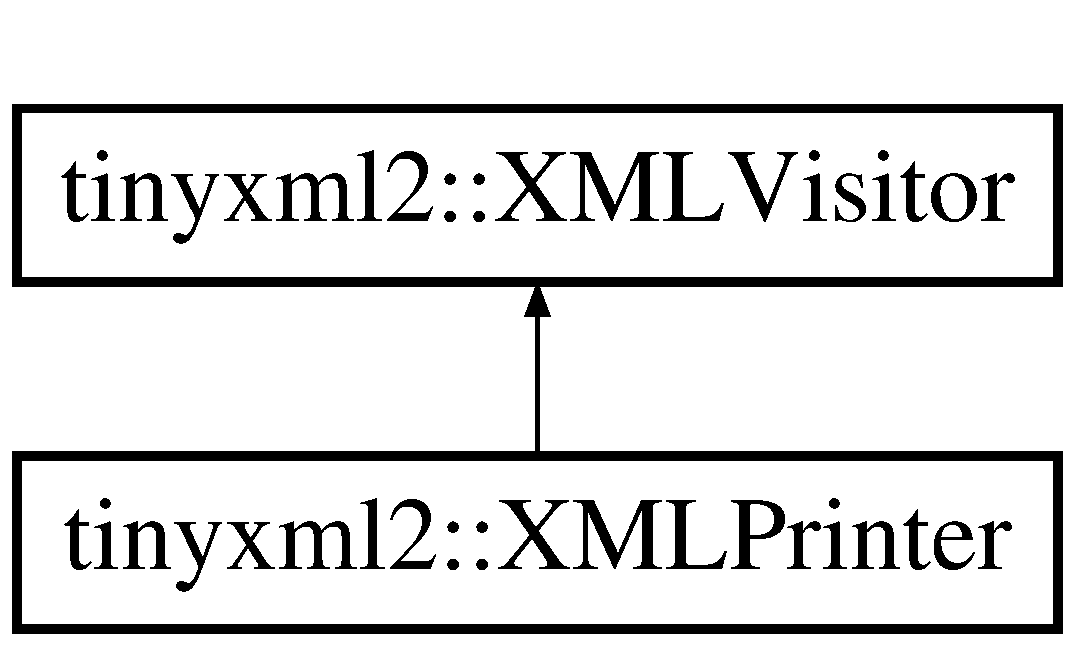
\includegraphics[height=2.000000cm]{classtinyxml2_1_1_x_m_l_printer}
\end{center}
\end{figure}
\subsection*{Public Member Functions}
\begin{DoxyCompactItemize}
\item 
\mbox{\hyperlink{classtinyxml2_1_1_x_m_l_printer_aa6d3841c069085f5b8a27bc7103c04f7}{X\+M\+L\+Printer}} (F\+I\+LE $\ast$file=0, bool compact=false, int depth=0)
\item 
void \mbox{\hyperlink{classtinyxml2_1_1_x_m_l_printer_a178c608ce8476043d5d6513819cde903}{Push\+Header}} (bool write\+B\+OM, bool write\+Declaration)
\item 
void \mbox{\hyperlink{classtinyxml2_1_1_x_m_l_printer_a20fb06c83bd13e5140d7dd13af06c010}{Open\+Element}} (const char $\ast$name, bool compact\+Mode=false)
\item 
\mbox{\Hypertarget{classtinyxml2_1_1_x_m_l_printer_a9a4e2c9348b42e147629d5a99f4af3f0}\label{classtinyxml2_1_1_x_m_l_printer_a9a4e2c9348b42e147629d5a99f4af3f0}} 
void \mbox{\hyperlink{classtinyxml2_1_1_x_m_l_printer_a9a4e2c9348b42e147629d5a99f4af3f0}{Push\+Attribute}} (const char $\ast$name, const char $\ast$value)
\begin{DoxyCompactList}\small\item\em If streaming, add an attribute to an open element. \end{DoxyCompactList}\item 
\mbox{\Hypertarget{classtinyxml2_1_1_x_m_l_printer_a69120c82088597372d28d0a98f2ee7a1}\label{classtinyxml2_1_1_x_m_l_printer_a69120c82088597372d28d0a98f2ee7a1}} 
void {\bfseries Push\+Attribute} (const char $\ast$name, int value)
\item 
\mbox{\Hypertarget{classtinyxml2_1_1_x_m_l_printer_aa41039e51990aaf5342f3e0575a692c4}\label{classtinyxml2_1_1_x_m_l_printer_aa41039e51990aaf5342f3e0575a692c4}} 
void {\bfseries Push\+Attribute} (const char $\ast$name, unsigned value)
\item 
\mbox{\Hypertarget{classtinyxml2_1_1_x_m_l_printer_a9bc2fe21a83a70e6aa0415f2034ecbff}\label{classtinyxml2_1_1_x_m_l_printer_a9bc2fe21a83a70e6aa0415f2034ecbff}} 
void {\bfseries Push\+Attribute} (const char $\ast$name, int64\+\_\+t value)
\item 
\mbox{\Hypertarget{classtinyxml2_1_1_x_m_l_printer_a51f7950d7b7a19f0d3a0d549a318d45f}\label{classtinyxml2_1_1_x_m_l_printer_a51f7950d7b7a19f0d3a0d549a318d45f}} 
void {\bfseries Push\+Attribute} (const char $\ast$name, bool value)
\item 
\mbox{\Hypertarget{classtinyxml2_1_1_x_m_l_printer_a1714867af40e68ca404c3e84b6cac2a6}\label{classtinyxml2_1_1_x_m_l_printer_a1714867af40e68ca404c3e84b6cac2a6}} 
void {\bfseries Push\+Attribute} (const char $\ast$name, double value)
\item 
\mbox{\Hypertarget{classtinyxml2_1_1_x_m_l_printer_af1fb439e5d800999646f333fa2f0699a}\label{classtinyxml2_1_1_x_m_l_printer_af1fb439e5d800999646f333fa2f0699a}} 
virtual void \mbox{\hyperlink{classtinyxml2_1_1_x_m_l_printer_af1fb439e5d800999646f333fa2f0699a}{Close\+Element}} (bool compact\+Mode=false)
\begin{DoxyCompactList}\small\item\em If streaming, close the Element. \end{DoxyCompactList}\item 
\mbox{\Hypertarget{classtinyxml2_1_1_x_m_l_printer_a1cc16a9362df4332012cb13cff6441b3}\label{classtinyxml2_1_1_x_m_l_printer_a1cc16a9362df4332012cb13cff6441b3}} 
void \mbox{\hyperlink{classtinyxml2_1_1_x_m_l_printer_a1cc16a9362df4332012cb13cff6441b3}{Push\+Text}} (const char $\ast$text, bool cdata=false)
\begin{DoxyCompactList}\small\item\em Add a text node. \end{DoxyCompactList}\item 
\mbox{\Hypertarget{classtinyxml2_1_1_x_m_l_printer_a3e0d4d78de25d4cf081009e1431cea7e}\label{classtinyxml2_1_1_x_m_l_printer_a3e0d4d78de25d4cf081009e1431cea7e}} 
void \mbox{\hyperlink{classtinyxml2_1_1_x_m_l_printer_a3e0d4d78de25d4cf081009e1431cea7e}{Push\+Text}} (int value)
\begin{DoxyCompactList}\small\item\em Add a text node from an integer. \end{DoxyCompactList}\item 
\mbox{\Hypertarget{classtinyxml2_1_1_x_m_l_printer_a661fb50e7e0a4918d2d259cb0fae647e}\label{classtinyxml2_1_1_x_m_l_printer_a661fb50e7e0a4918d2d259cb0fae647e}} 
void \mbox{\hyperlink{classtinyxml2_1_1_x_m_l_printer_a661fb50e7e0a4918d2d259cb0fae647e}{Push\+Text}} (unsigned value)
\begin{DoxyCompactList}\small\item\em Add a text node from an unsigned. \end{DoxyCompactList}\item 
\mbox{\Hypertarget{classtinyxml2_1_1_x_m_l_printer_a96b0a0bfe105154a0a6c37d725258f0a}\label{classtinyxml2_1_1_x_m_l_printer_a96b0a0bfe105154a0a6c37d725258f0a}} 
void \mbox{\hyperlink{classtinyxml2_1_1_x_m_l_printer_a96b0a0bfe105154a0a6c37d725258f0a}{Push\+Text}} (int64\+\_\+t value)
\begin{DoxyCompactList}\small\item\em Add a text node from an unsigned. \end{DoxyCompactList}\item 
\mbox{\Hypertarget{classtinyxml2_1_1_x_m_l_printer_a4390e5fa1ed05189a8686647345ab29f}\label{classtinyxml2_1_1_x_m_l_printer_a4390e5fa1ed05189a8686647345ab29f}} 
void \mbox{\hyperlink{classtinyxml2_1_1_x_m_l_printer_a4390e5fa1ed05189a8686647345ab29f}{Push\+Text}} (bool value)
\begin{DoxyCompactList}\small\item\em Add a text node from a bool. \end{DoxyCompactList}\item 
\mbox{\Hypertarget{classtinyxml2_1_1_x_m_l_printer_a1dbb1390e829d0673af66b9cd1928bd7}\label{classtinyxml2_1_1_x_m_l_printer_a1dbb1390e829d0673af66b9cd1928bd7}} 
void \mbox{\hyperlink{classtinyxml2_1_1_x_m_l_printer_a1dbb1390e829d0673af66b9cd1928bd7}{Push\+Text}} (float value)
\begin{DoxyCompactList}\small\item\em Add a text node from a float. \end{DoxyCompactList}\item 
\mbox{\Hypertarget{classtinyxml2_1_1_x_m_l_printer_aa715302dfc09473c77c853cbd5431965}\label{classtinyxml2_1_1_x_m_l_printer_aa715302dfc09473c77c853cbd5431965}} 
void \mbox{\hyperlink{classtinyxml2_1_1_x_m_l_printer_aa715302dfc09473c77c853cbd5431965}{Push\+Text}} (double value)
\begin{DoxyCompactList}\small\item\em Add a text node from a double. \end{DoxyCompactList}\item 
\mbox{\Hypertarget{classtinyxml2_1_1_x_m_l_printer_afc8416814219591c2fd5656e0c233140}\label{classtinyxml2_1_1_x_m_l_printer_afc8416814219591c2fd5656e0c233140}} 
void \mbox{\hyperlink{classtinyxml2_1_1_x_m_l_printer_afc8416814219591c2fd5656e0c233140}{Push\+Comment}} (const char $\ast$comment)
\begin{DoxyCompactList}\small\item\em Add a comment. \end{DoxyCompactList}\item 
\mbox{\Hypertarget{classtinyxml2_1_1_x_m_l_printer_a2fe3565e262594efc6c0276723c83fe7}\label{classtinyxml2_1_1_x_m_l_printer_a2fe3565e262594efc6c0276723c83fe7}} 
void {\bfseries Push\+Declaration} (const char $\ast$value)
\item 
\mbox{\Hypertarget{classtinyxml2_1_1_x_m_l_printer_ab1efc6d1548505e9984185f58f54b713}\label{classtinyxml2_1_1_x_m_l_printer_ab1efc6d1548505e9984185f58f54b713}} 
void {\bfseries Push\+Unknown} (const char $\ast$value)
\item 
\mbox{\Hypertarget{classtinyxml2_1_1_x_m_l_printer_a9aa1de11a55a07db55a90fde37d7afad}\label{classtinyxml2_1_1_x_m_l_printer_a9aa1de11a55a07db55a90fde37d7afad}} 
virtual bool \mbox{\hyperlink{classtinyxml2_1_1_x_m_l_printer_a9aa1de11a55a07db55a90fde37d7afad}{Visit\+Enter}} (const \mbox{\hyperlink{classtinyxml2_1_1_x_m_l_document}{X\+M\+L\+Document}} \&)
\begin{DoxyCompactList}\small\item\em Visit a document. \end{DoxyCompactList}\item 
\mbox{\Hypertarget{classtinyxml2_1_1_x_m_l_printer_a15fc1f2b922f540917dcf52808737b29}\label{classtinyxml2_1_1_x_m_l_printer_a15fc1f2b922f540917dcf52808737b29}} 
virtual bool \mbox{\hyperlink{classtinyxml2_1_1_x_m_l_printer_a15fc1f2b922f540917dcf52808737b29}{Visit\+Exit}} (const \mbox{\hyperlink{classtinyxml2_1_1_x_m_l_document}{X\+M\+L\+Document}} \&)
\begin{DoxyCompactList}\small\item\em Visit a document. \end{DoxyCompactList}\item 
\mbox{\Hypertarget{classtinyxml2_1_1_x_m_l_printer_a169b2509d8eabb70811b2bb8cfd1f5d1}\label{classtinyxml2_1_1_x_m_l_printer_a169b2509d8eabb70811b2bb8cfd1f5d1}} 
virtual bool \mbox{\hyperlink{classtinyxml2_1_1_x_m_l_printer_a169b2509d8eabb70811b2bb8cfd1f5d1}{Visit\+Enter}} (const \mbox{\hyperlink{classtinyxml2_1_1_x_m_l_element}{X\+M\+L\+Element}} \&element, const \mbox{\hyperlink{classtinyxml2_1_1_x_m_l_attribute}{X\+M\+L\+Attribute}} $\ast$attribute)
\begin{DoxyCompactList}\small\item\em Visit an element. \end{DoxyCompactList}\item 
\mbox{\Hypertarget{classtinyxml2_1_1_x_m_l_printer_a2edd48405971a88951c71c9df86a2f50}\label{classtinyxml2_1_1_x_m_l_printer_a2edd48405971a88951c71c9df86a2f50}} 
virtual bool \mbox{\hyperlink{classtinyxml2_1_1_x_m_l_printer_a2edd48405971a88951c71c9df86a2f50}{Visit\+Exit}} (const \mbox{\hyperlink{classtinyxml2_1_1_x_m_l_element}{X\+M\+L\+Element}} \&element)
\begin{DoxyCompactList}\small\item\em Visit an element. \end{DoxyCompactList}\item 
\mbox{\Hypertarget{classtinyxml2_1_1_x_m_l_printer_adc0e42b4f6fcb90a95630c79575d030b}\label{classtinyxml2_1_1_x_m_l_printer_adc0e42b4f6fcb90a95630c79575d030b}} 
virtual bool \mbox{\hyperlink{classtinyxml2_1_1_x_m_l_printer_adc0e42b4f6fcb90a95630c79575d030b}{Visit}} (const \mbox{\hyperlink{classtinyxml2_1_1_x_m_l_text}{X\+M\+L\+Text}} \&text)
\begin{DoxyCompactList}\small\item\em Visit a text node. \end{DoxyCompactList}\item 
\mbox{\Hypertarget{classtinyxml2_1_1_x_m_l_printer_aa294c5c01af0ebb9114902456e4cb53c}\label{classtinyxml2_1_1_x_m_l_printer_aa294c5c01af0ebb9114902456e4cb53c}} 
virtual bool \mbox{\hyperlink{classtinyxml2_1_1_x_m_l_printer_aa294c5c01af0ebb9114902456e4cb53c}{Visit}} (const \mbox{\hyperlink{classtinyxml2_1_1_x_m_l_comment}{X\+M\+L\+Comment}} \&comment)
\begin{DoxyCompactList}\small\item\em Visit a comment node. \end{DoxyCompactList}\item 
\mbox{\Hypertarget{classtinyxml2_1_1_x_m_l_printer_acfc625b2549304b9c7eb85ebd5c5eb39}\label{classtinyxml2_1_1_x_m_l_printer_acfc625b2549304b9c7eb85ebd5c5eb39}} 
virtual bool \mbox{\hyperlink{classtinyxml2_1_1_x_m_l_printer_acfc625b2549304b9c7eb85ebd5c5eb39}{Visit}} (const \mbox{\hyperlink{classtinyxml2_1_1_x_m_l_declaration}{X\+M\+L\+Declaration}} \&declaration)
\begin{DoxyCompactList}\small\item\em Visit a declaration. \end{DoxyCompactList}\item 
\mbox{\Hypertarget{classtinyxml2_1_1_x_m_l_printer_ab8af5455bbf9e4be2663e6642fcd7e32}\label{classtinyxml2_1_1_x_m_l_printer_ab8af5455bbf9e4be2663e6642fcd7e32}} 
virtual bool \mbox{\hyperlink{classtinyxml2_1_1_x_m_l_printer_ab8af5455bbf9e4be2663e6642fcd7e32}{Visit}} (const \mbox{\hyperlink{classtinyxml2_1_1_x_m_l_unknown}{X\+M\+L\+Unknown}} \&unknown)
\begin{DoxyCompactList}\small\item\em Visit an unknown node. \end{DoxyCompactList}\item 
const char $\ast$ \mbox{\hyperlink{classtinyxml2_1_1_x_m_l_printer_a180671d73844f159f2d4aafbc11d106e}{C\+Str}} () const
\item 
int \mbox{\hyperlink{classtinyxml2_1_1_x_m_l_printer_a3256cf3523d4898b91abb18b924be04c}{C\+Str\+Size}} () const
\item 
void \mbox{\hyperlink{classtinyxml2_1_1_x_m_l_printer_a216157765b7267bf389975b1cbf9a909}{Clear\+Buffer}} ()
\end{DoxyCompactItemize}
\subsection*{Protected Member Functions}
\begin{DoxyCompactItemize}
\item 
\mbox{\Hypertarget{classtinyxml2_1_1_x_m_l_printer_a38e1ed5a779bdf63eda9e808f7a6de66}\label{classtinyxml2_1_1_x_m_l_printer_a38e1ed5a779bdf63eda9e808f7a6de66}} 
virtual bool {\bfseries Compact\+Mode} (const \mbox{\hyperlink{classtinyxml2_1_1_x_m_l_element}{X\+M\+L\+Element}} \&)
\item 
virtual void \mbox{\hyperlink{classtinyxml2_1_1_x_m_l_printer_a1c4b2ccbe4fdb316d54f5a93f3559260}{Print\+Space}} (int depth)
\item 
\mbox{\Hypertarget{classtinyxml2_1_1_x_m_l_printer_ab30210a7f32e45634e7a45137bf6fdf6}\label{classtinyxml2_1_1_x_m_l_printer_ab30210a7f32e45634e7a45137bf6fdf6}} 
void {\bfseries Print} (const char $\ast$format,...)
\item 
\mbox{\Hypertarget{classtinyxml2_1_1_x_m_l_printer_aff363b7634a27538fd691ae62adbda63}\label{classtinyxml2_1_1_x_m_l_printer_aff363b7634a27538fd691ae62adbda63}} 
void {\bfseries Write} (const char $\ast$data, size\+\_\+t size)
\item 
\mbox{\Hypertarget{classtinyxml2_1_1_x_m_l_printer_a4bd7f0cabca77ac95c299103fa9592f1}\label{classtinyxml2_1_1_x_m_l_printer_a4bd7f0cabca77ac95c299103fa9592f1}} 
void {\bfseries Write} (const char $\ast$data)
\item 
\mbox{\Hypertarget{classtinyxml2_1_1_x_m_l_printer_a9567b0218169ba59794f171ae2f9944c}\label{classtinyxml2_1_1_x_m_l_printer_a9567b0218169ba59794f171ae2f9944c}} 
void {\bfseries Putc} (char ch)
\item 
\mbox{\Hypertarget{classtinyxml2_1_1_x_m_l_printer_ac6e2c72c5d796f5b4de6ce81ca95e3fa}\label{classtinyxml2_1_1_x_m_l_printer_ac6e2c72c5d796f5b4de6ce81ca95e3fa}} 
void {\bfseries Seal\+Element\+If\+Just\+Opened} ()
\end{DoxyCompactItemize}
\subsection*{Protected Attributes}
\begin{DoxyCompactItemize}
\item 
\mbox{\Hypertarget{classtinyxml2_1_1_x_m_l_printer_ac07169d58b465214a2b1fa306e617c26}\label{classtinyxml2_1_1_x_m_l_printer_ac07169d58b465214a2b1fa306e617c26}} 
bool {\bfseries \+\_\+element\+Just\+Opened}
\item 
\mbox{\Hypertarget{classtinyxml2_1_1_x_m_l_printer_a99d59e67e084714541bee3ae43884bef}\label{classtinyxml2_1_1_x_m_l_printer_a99d59e67e084714541bee3ae43884bef}} 
\mbox{\hyperlink{classtinyxml2_1_1_dyn_array}{Dyn\+Array}}$<$ const char $\ast$, 10 $>$ {\bfseries \+\_\+stack}
\end{DoxyCompactItemize}


\subsection{Detailed Description}
Printing functionality. The \mbox{\hyperlink{classtinyxml2_1_1_x_m_l_printer}{X\+M\+L\+Printer}} gives you more options than the \mbox{\hyperlink{classtinyxml2_1_1_x_m_l_document_a867cf5fa3e3ff6ae4847a8b7ee8ec083}{X\+M\+L\+Document\+::\+Print()}} method.

It can\+:
\begin{DoxyEnumerate}
\item Print to memory.
\item Print to a file you provide.
\item Print X\+ML without a \mbox{\hyperlink{classtinyxml2_1_1_x_m_l_document}{X\+M\+L\+Document}}.
\end{DoxyEnumerate}

Print to Memory

\begin{DoxyVerb}XMLPrinter printer;
doc.Print( &printer );
SomeFunction( printer.CStr() );
\end{DoxyVerb}


Print to a File

You provide the file pointer. \begin{DoxyVerb}XMLPrinter printer( fp );
doc.Print( &printer );
\end{DoxyVerb}


Print without a \mbox{\hyperlink{classtinyxml2_1_1_x_m_l_document}{X\+M\+L\+Document}}

When loading, an X\+ML parser is very useful. However, sometimes when saving, it just gets in the way. The code is often set up for streaming, and constructing the D\+OM is just overhead.

The Printer supports the streaming case. The following code prints out a trivially simple X\+ML file without ever creating an X\+ML document.

\begin{DoxyVerb}XMLPrinter printer( fp );
printer.OpenElement( "foo" );
printer.PushAttribute( "foo", "bar" );
printer.CloseElement();
\end{DoxyVerb}
 

\subsection{Constructor \& Destructor Documentation}
\mbox{\Hypertarget{classtinyxml2_1_1_x_m_l_printer_aa6d3841c069085f5b8a27bc7103c04f7}\label{classtinyxml2_1_1_x_m_l_printer_aa6d3841c069085f5b8a27bc7103c04f7}} 
\index{tinyxml2\+::\+X\+M\+L\+Printer@{tinyxml2\+::\+X\+M\+L\+Printer}!X\+M\+L\+Printer@{X\+M\+L\+Printer}}
\index{X\+M\+L\+Printer@{X\+M\+L\+Printer}!tinyxml2\+::\+X\+M\+L\+Printer@{tinyxml2\+::\+X\+M\+L\+Printer}}
\subsubsection{\texorpdfstring{X\+M\+L\+Printer()}{XMLPrinter()}}
{\footnotesize\ttfamily tinyxml2\+::\+X\+M\+L\+Printer\+::\+X\+M\+L\+Printer (\begin{DoxyParamCaption}\item[{F\+I\+LE $\ast$}]{file = {\ttfamily 0},  }\item[{bool}]{compact = {\ttfamily false},  }\item[{int}]{depth = {\ttfamily 0} }\end{DoxyParamCaption})}

Construct the printer. If the F\+I\+L\+E$\ast$ is specified, this will print to the F\+I\+LE. Else it will print to memory, and the result is available in \mbox{\hyperlink{classtinyxml2_1_1_x_m_l_printer_a180671d73844f159f2d4aafbc11d106e}{C\+Str()}}. If \textquotesingle{}compact\textquotesingle{} is set to true, then output is created with only required whitespace and newlines. 

\subsection{Member Function Documentation}
\mbox{\Hypertarget{classtinyxml2_1_1_x_m_l_printer_a216157765b7267bf389975b1cbf9a909}\label{classtinyxml2_1_1_x_m_l_printer_a216157765b7267bf389975b1cbf9a909}} 
\index{tinyxml2\+::\+X\+M\+L\+Printer@{tinyxml2\+::\+X\+M\+L\+Printer}!Clear\+Buffer@{Clear\+Buffer}}
\index{Clear\+Buffer@{Clear\+Buffer}!tinyxml2\+::\+X\+M\+L\+Printer@{tinyxml2\+::\+X\+M\+L\+Printer}}
\subsubsection{\texorpdfstring{Clear\+Buffer()}{ClearBuffer()}}
{\footnotesize\ttfamily void tinyxml2\+::\+X\+M\+L\+Printer\+::\+Clear\+Buffer (\begin{DoxyParamCaption}{ }\end{DoxyParamCaption})\hspace{0.3cm}{\ttfamily [inline]}}

If in print to memory mode, reset the buffer to the beginning. \mbox{\Hypertarget{classtinyxml2_1_1_x_m_l_printer_a180671d73844f159f2d4aafbc11d106e}\label{classtinyxml2_1_1_x_m_l_printer_a180671d73844f159f2d4aafbc11d106e}} 
\index{tinyxml2\+::\+X\+M\+L\+Printer@{tinyxml2\+::\+X\+M\+L\+Printer}!C\+Str@{C\+Str}}
\index{C\+Str@{C\+Str}!tinyxml2\+::\+X\+M\+L\+Printer@{tinyxml2\+::\+X\+M\+L\+Printer}}
\subsubsection{\texorpdfstring{C\+Str()}{CStr()}}
{\footnotesize\ttfamily const char$\ast$ tinyxml2\+::\+X\+M\+L\+Printer\+::\+C\+Str (\begin{DoxyParamCaption}{ }\end{DoxyParamCaption}) const\hspace{0.3cm}{\ttfamily [inline]}}

If in print to memory mode, return a pointer to the X\+ML file in memory. \mbox{\Hypertarget{classtinyxml2_1_1_x_m_l_printer_a3256cf3523d4898b91abb18b924be04c}\label{classtinyxml2_1_1_x_m_l_printer_a3256cf3523d4898b91abb18b924be04c}} 
\index{tinyxml2\+::\+X\+M\+L\+Printer@{tinyxml2\+::\+X\+M\+L\+Printer}!C\+Str\+Size@{C\+Str\+Size}}
\index{C\+Str\+Size@{C\+Str\+Size}!tinyxml2\+::\+X\+M\+L\+Printer@{tinyxml2\+::\+X\+M\+L\+Printer}}
\subsubsection{\texorpdfstring{C\+Str\+Size()}{CStrSize()}}
{\footnotesize\ttfamily int tinyxml2\+::\+X\+M\+L\+Printer\+::\+C\+Str\+Size (\begin{DoxyParamCaption}{ }\end{DoxyParamCaption}) const\hspace{0.3cm}{\ttfamily [inline]}}

If in print to memory mode, return the size of the X\+ML file in memory. (Note the size returned includes the terminating null.) \mbox{\Hypertarget{classtinyxml2_1_1_x_m_l_printer_a20fb06c83bd13e5140d7dd13af06c010}\label{classtinyxml2_1_1_x_m_l_printer_a20fb06c83bd13e5140d7dd13af06c010}} 
\index{tinyxml2\+::\+X\+M\+L\+Printer@{tinyxml2\+::\+X\+M\+L\+Printer}!Open\+Element@{Open\+Element}}
\index{Open\+Element@{Open\+Element}!tinyxml2\+::\+X\+M\+L\+Printer@{tinyxml2\+::\+X\+M\+L\+Printer}}
\subsubsection{\texorpdfstring{Open\+Element()}{OpenElement()}}
{\footnotesize\ttfamily void tinyxml2\+::\+X\+M\+L\+Printer\+::\+Open\+Element (\begin{DoxyParamCaption}\item[{const char $\ast$}]{name,  }\item[{bool}]{compact\+Mode = {\ttfamily false} }\end{DoxyParamCaption})}

If streaming, start writing an element. The element must be closed with \mbox{\hyperlink{classtinyxml2_1_1_x_m_l_printer_af1fb439e5d800999646f333fa2f0699a}{Close\+Element()}} \mbox{\Hypertarget{classtinyxml2_1_1_x_m_l_printer_a1c4b2ccbe4fdb316d54f5a93f3559260}\label{classtinyxml2_1_1_x_m_l_printer_a1c4b2ccbe4fdb316d54f5a93f3559260}} 
\index{tinyxml2\+::\+X\+M\+L\+Printer@{tinyxml2\+::\+X\+M\+L\+Printer}!Print\+Space@{Print\+Space}}
\index{Print\+Space@{Print\+Space}!tinyxml2\+::\+X\+M\+L\+Printer@{tinyxml2\+::\+X\+M\+L\+Printer}}
\subsubsection{\texorpdfstring{Print\+Space()}{PrintSpace()}}
{\footnotesize\ttfamily void tinyxml2\+::\+X\+M\+L\+Printer\+::\+Print\+Space (\begin{DoxyParamCaption}\item[{int}]{depth }\end{DoxyParamCaption})\hspace{0.3cm}{\ttfamily [protected]}, {\ttfamily [virtual]}}

Prints out the space before an element. You may override to change the space and tabs used. A \mbox{\hyperlink{classtinyxml2_1_1_x_m_l_printer_a1c4b2ccbe4fdb316d54f5a93f3559260}{Print\+Space()}} override should call Print(). \mbox{\Hypertarget{classtinyxml2_1_1_x_m_l_printer_a178c608ce8476043d5d6513819cde903}\label{classtinyxml2_1_1_x_m_l_printer_a178c608ce8476043d5d6513819cde903}} 
\index{tinyxml2\+::\+X\+M\+L\+Printer@{tinyxml2\+::\+X\+M\+L\+Printer}!Push\+Header@{Push\+Header}}
\index{Push\+Header@{Push\+Header}!tinyxml2\+::\+X\+M\+L\+Printer@{tinyxml2\+::\+X\+M\+L\+Printer}}
\subsubsection{\texorpdfstring{Push\+Header()}{PushHeader()}}
{\footnotesize\ttfamily void tinyxml2\+::\+X\+M\+L\+Printer\+::\+Push\+Header (\begin{DoxyParamCaption}\item[{bool}]{write\+B\+OM,  }\item[{bool}]{write\+Declaration }\end{DoxyParamCaption})}

If streaming, write the B\+OM and declaration. 

The documentation for this class was generated from the following files\+:\begin{DoxyCompactItemize}
\item 
Source/\+Utils/tinyxml2.\+h\item 
Source/\+Utils/tinyxml2.\+cpp\end{DoxyCompactItemize}

\hypertarget{classtinyxml2_1_1_x_m_l_text}{}\section{tinyxml2\+:\+:X\+M\+L\+Text Class Reference}
\label{classtinyxml2_1_1_x_m_l_text}\index{tinyxml2\+::\+X\+M\+L\+Text@{tinyxml2\+::\+X\+M\+L\+Text}}


{\ttfamily \#include $<$tinyxml2.\+h$>$}

Inheritance diagram for tinyxml2\+:\+:X\+M\+L\+Text\+:\begin{figure}[H]
\begin{center}
\leavevmode
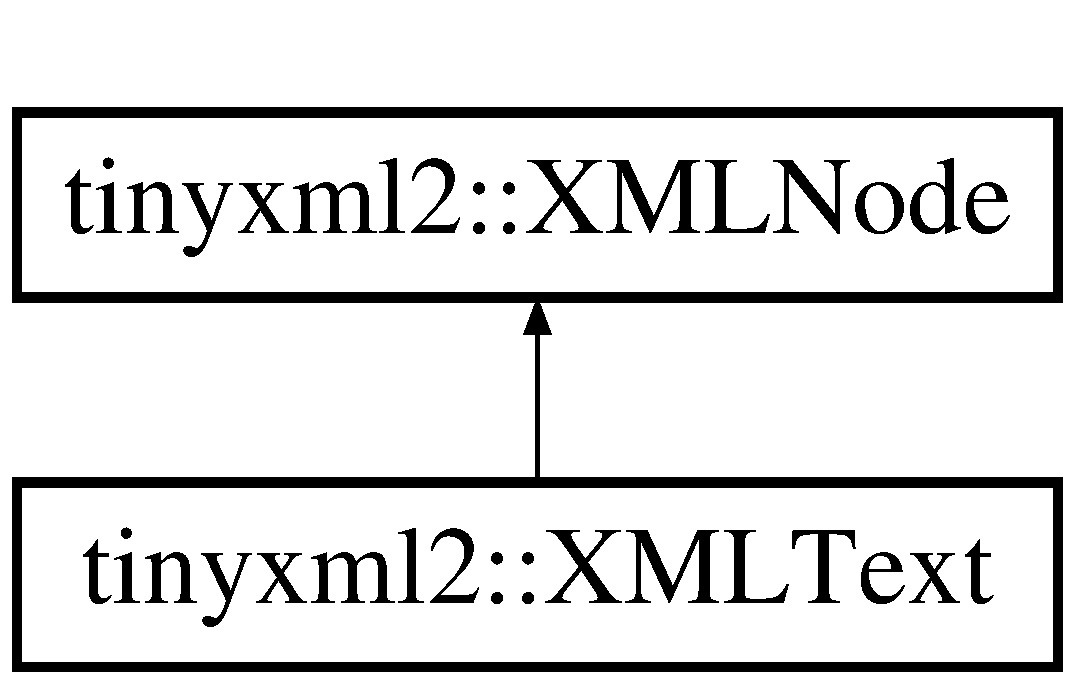
\includegraphics[height=2.000000cm]{classtinyxml2_1_1_x_m_l_text}
\end{center}
\end{figure}
\subsection*{Public Member Functions}
\begin{DoxyCompactItemize}
\item 
virtual bool \mbox{\hyperlink{classtinyxml2_1_1_x_m_l_text_a537c60d7e18fb59c45ac2737a29ac47a}{Accept}} (\mbox{\hyperlink{classtinyxml2_1_1_x_m_l_visitor}{X\+M\+L\+Visitor}} $\ast$visitor) const
\item 
\mbox{\Hypertarget{classtinyxml2_1_1_x_m_l_text_ab1213b4ddebe9b17ec7e7040e9f1caf7}\label{classtinyxml2_1_1_x_m_l_text_ab1213b4ddebe9b17ec7e7040e9f1caf7}} 
virtual \mbox{\hyperlink{classtinyxml2_1_1_x_m_l_text}{X\+M\+L\+Text}} $\ast$ \mbox{\hyperlink{classtinyxml2_1_1_x_m_l_text_ab1213b4ddebe9b17ec7e7040e9f1caf7}{To\+Text}} ()
\begin{DoxyCompactList}\small\item\em Safely cast to Text, or null. \end{DoxyCompactList}\item 
\mbox{\Hypertarget{classtinyxml2_1_1_x_m_l_text_a671ce22c7c5ef378f1ce31e6f827b9e2}\label{classtinyxml2_1_1_x_m_l_text_a671ce22c7c5ef378f1ce31e6f827b9e2}} 
virtual const \mbox{\hyperlink{classtinyxml2_1_1_x_m_l_text}{X\+M\+L\+Text}} $\ast$ {\bfseries To\+Text} () const
\item 
\mbox{\Hypertarget{classtinyxml2_1_1_x_m_l_text_ad080357d76ab7cc59d7651249949329d}\label{classtinyxml2_1_1_x_m_l_text_ad080357d76ab7cc59d7651249949329d}} 
void \mbox{\hyperlink{classtinyxml2_1_1_x_m_l_text_ad080357d76ab7cc59d7651249949329d}{Set\+C\+Data}} (bool is\+C\+Data)
\begin{DoxyCompactList}\small\item\em Declare whether this should be C\+D\+A\+TA or standard text. \end{DoxyCompactList}\item 
\mbox{\Hypertarget{classtinyxml2_1_1_x_m_l_text_ac1bb5ea4166c320882d9e0ad16fd385b}\label{classtinyxml2_1_1_x_m_l_text_ac1bb5ea4166c320882d9e0ad16fd385b}} 
bool \mbox{\hyperlink{classtinyxml2_1_1_x_m_l_text_ac1bb5ea4166c320882d9e0ad16fd385b}{C\+Data}} () const
\begin{DoxyCompactList}\small\item\em Returns true if this is a C\+D\+A\+TA text element. \end{DoxyCompactList}\item 
virtual \mbox{\hyperlink{classtinyxml2_1_1_x_m_l_node}{X\+M\+L\+Node}} $\ast$ \mbox{\hyperlink{classtinyxml2_1_1_x_m_l_text_a86d265c93152726c8c6831e9594840e6}{Shallow\+Clone}} (\mbox{\hyperlink{classtinyxml2_1_1_x_m_l_document}{X\+M\+L\+Document}} $\ast$document) const
\item 
virtual bool \mbox{\hyperlink{classtinyxml2_1_1_x_m_l_text_a99d8bce4dc01df889126e047f358cdfc}{Shallow\+Equal}} (const \mbox{\hyperlink{classtinyxml2_1_1_x_m_l_node}{X\+M\+L\+Node}} $\ast$compare) const
\end{DoxyCompactItemize}
\subsection*{Protected Member Functions}
\begin{DoxyCompactItemize}
\item 
\mbox{\Hypertarget{classtinyxml2_1_1_x_m_l_text_ad9f46d70e61e5386ead93728d8b90267}\label{classtinyxml2_1_1_x_m_l_text_ad9f46d70e61e5386ead93728d8b90267}} 
{\bfseries X\+M\+L\+Text} (\mbox{\hyperlink{classtinyxml2_1_1_x_m_l_document}{X\+M\+L\+Document}} $\ast$doc)
\item 
\mbox{\Hypertarget{classtinyxml2_1_1_x_m_l_text_af3b93344f1183482e1683f5922ac9c68}\label{classtinyxml2_1_1_x_m_l_text_af3b93344f1183482e1683f5922ac9c68}} 
char $\ast$ {\bfseries Parse\+Deep} (char $\ast$p, \mbox{\hyperlink{classtinyxml2_1_1_str_pair}{Str\+Pair}} $\ast$parent\+End\+Tag, int $\ast$cur\+Line\+Num\+Ptr)
\end{DoxyCompactItemize}
\subsection*{Friends}
\begin{DoxyCompactItemize}
\item 
\mbox{\Hypertarget{classtinyxml2_1_1_x_m_l_text_a4eee3bda60c60a30e4e8cd4ea91c4c6e}\label{classtinyxml2_1_1_x_m_l_text_a4eee3bda60c60a30e4e8cd4ea91c4c6e}} 
class {\bfseries X\+M\+L\+Document}
\end{DoxyCompactItemize}
\subsection*{Additional Inherited Members}


\subsection{Detailed Description}
X\+ML text.

Note that a text node can have child element nodes, for example\+: \begin{DoxyVerb}<root>This is <b>bold</b></root>
\end{DoxyVerb}


A text node can have 2 ways to output the next. \char`\"{}normal\char`\"{} output and C\+D\+A\+TA. It will default to the mode it was parsed from the X\+ML file and you generally want to leave it alone, but you can change the output mode with \mbox{\hyperlink{classtinyxml2_1_1_x_m_l_text_ad080357d76ab7cc59d7651249949329d}{Set\+C\+Data()}} and query it with \mbox{\hyperlink{classtinyxml2_1_1_x_m_l_text_ac1bb5ea4166c320882d9e0ad16fd385b}{C\+Data()}}. 

\subsection{Member Function Documentation}
\mbox{\Hypertarget{classtinyxml2_1_1_x_m_l_text_a537c60d7e18fb59c45ac2737a29ac47a}\label{classtinyxml2_1_1_x_m_l_text_a537c60d7e18fb59c45ac2737a29ac47a}} 
\index{tinyxml2\+::\+X\+M\+L\+Text@{tinyxml2\+::\+X\+M\+L\+Text}!Accept@{Accept}}
\index{Accept@{Accept}!tinyxml2\+::\+X\+M\+L\+Text@{tinyxml2\+::\+X\+M\+L\+Text}}
\subsubsection{\texorpdfstring{Accept()}{Accept()}}
{\footnotesize\ttfamily bool tinyxml2\+::\+X\+M\+L\+Text\+::\+Accept (\begin{DoxyParamCaption}\item[{\mbox{\hyperlink{classtinyxml2_1_1_x_m_l_visitor}{X\+M\+L\+Visitor}} $\ast$}]{visitor }\end{DoxyParamCaption}) const\hspace{0.3cm}{\ttfamily [virtual]}}

Accept a hierarchical visit of the nodes in the Tiny\+X\+M\+L-\/2 D\+OM. Every node in the X\+ML tree will be conditionally visited and the host will be called back via the \mbox{\hyperlink{classtinyxml2_1_1_x_m_l_visitor}{X\+M\+L\+Visitor}} interface.

This is essentially a S\+AX interface for Tiny\+X\+M\+L-\/2. (Note however it doesn\textquotesingle{}t re-\/parse the X\+ML for the callbacks, so the performance of Tiny\+X\+M\+L-\/2 is unchanged by using this interface versus any other.)

The interface has been based on ideas from\+:


\begin{DoxyItemize}
\item \href{http://www.saxproject.org/}{\tt http\+://www.\+saxproject.\+org/}
\item \href{http://c2.com/cgi/wiki?HierarchicalVisitorPattern}{\tt http\+://c2.\+com/cgi/wiki?\+Hierarchical\+Visitor\+Pattern}
\end{DoxyItemize}

Which are both good references for \char`\"{}visiting\char`\"{}.

An example of using \mbox{\hyperlink{classtinyxml2_1_1_x_m_l_text_a537c60d7e18fb59c45ac2737a29ac47a}{Accept()}}\+: \begin{DoxyVerb}XMLPrinter printer;
tinyxmlDoc.Accept( &printer );
const char* xmlcstr = printer.CStr();
\end{DoxyVerb}
 

Implements \mbox{\hyperlink{classtinyxml2_1_1_x_m_l_node_a81e66df0a44c67a7af17f3b77a152785}{tinyxml2\+::\+X\+M\+L\+Node}}.

\mbox{\Hypertarget{classtinyxml2_1_1_x_m_l_text_a86d265c93152726c8c6831e9594840e6}\label{classtinyxml2_1_1_x_m_l_text_a86d265c93152726c8c6831e9594840e6}} 
\index{tinyxml2\+::\+X\+M\+L\+Text@{tinyxml2\+::\+X\+M\+L\+Text}!Shallow\+Clone@{Shallow\+Clone}}
\index{Shallow\+Clone@{Shallow\+Clone}!tinyxml2\+::\+X\+M\+L\+Text@{tinyxml2\+::\+X\+M\+L\+Text}}
\subsubsection{\texorpdfstring{Shallow\+Clone()}{ShallowClone()}}
{\footnotesize\ttfamily \mbox{\hyperlink{classtinyxml2_1_1_x_m_l_node}{X\+M\+L\+Node}} $\ast$ tinyxml2\+::\+X\+M\+L\+Text\+::\+Shallow\+Clone (\begin{DoxyParamCaption}\item[{\mbox{\hyperlink{classtinyxml2_1_1_x_m_l_document}{X\+M\+L\+Document}} $\ast$}]{document }\end{DoxyParamCaption}) const\hspace{0.3cm}{\ttfamily [virtual]}}

Make a copy of this node, but not its children. You may pass in a Document pointer that will be the owner of the new Node. If the \textquotesingle{}document\textquotesingle{} is null, then the node returned will be allocated from the current Document. (this-\/$>$\mbox{\hyperlink{classtinyxml2_1_1_x_m_l_node_af343d1ef0b45c0020e62d784d7e67a68}{Get\+Document()}})

Note\+: if called on a \mbox{\hyperlink{classtinyxml2_1_1_x_m_l_document}{X\+M\+L\+Document}}, this will return null. 

Implements \mbox{\hyperlink{classtinyxml2_1_1_x_m_l_node_a8402cbd3129d20e9e6024bbcc0531283}{tinyxml2\+::\+X\+M\+L\+Node}}.

\mbox{\Hypertarget{classtinyxml2_1_1_x_m_l_text_a99d8bce4dc01df889126e047f358cdfc}\label{classtinyxml2_1_1_x_m_l_text_a99d8bce4dc01df889126e047f358cdfc}} 
\index{tinyxml2\+::\+X\+M\+L\+Text@{tinyxml2\+::\+X\+M\+L\+Text}!Shallow\+Equal@{Shallow\+Equal}}
\index{Shallow\+Equal@{Shallow\+Equal}!tinyxml2\+::\+X\+M\+L\+Text@{tinyxml2\+::\+X\+M\+L\+Text}}
\subsubsection{\texorpdfstring{Shallow\+Equal()}{ShallowEqual()}}
{\footnotesize\ttfamily bool tinyxml2\+::\+X\+M\+L\+Text\+::\+Shallow\+Equal (\begin{DoxyParamCaption}\item[{const \mbox{\hyperlink{classtinyxml2_1_1_x_m_l_node}{X\+M\+L\+Node}} $\ast$}]{compare }\end{DoxyParamCaption}) const\hspace{0.3cm}{\ttfamily [virtual]}}

Test if 2 nodes are the same, but don\textquotesingle{}t test children. The 2 nodes do not need to be in the same Document.

Note\+: if called on a \mbox{\hyperlink{classtinyxml2_1_1_x_m_l_document}{X\+M\+L\+Document}}, this will return false. 

Implements \mbox{\hyperlink{classtinyxml2_1_1_x_m_l_node_a7ce18b751c3ea09eac292dca264f9226}{tinyxml2\+::\+X\+M\+L\+Node}}.



The documentation for this class was generated from the following files\+:\begin{DoxyCompactItemize}
\item 
Source/\+Utils/tinyxml2.\+h\item 
Source/\+Utils/tinyxml2.\+cpp\end{DoxyCompactItemize}

\hypertarget{classtinyxml2_1_1_x_m_l_unknown}{}\section{tinyxml2\+:\+:X\+M\+L\+Unknown Class Reference}
\label{classtinyxml2_1_1_x_m_l_unknown}\index{tinyxml2\+::\+X\+M\+L\+Unknown@{tinyxml2\+::\+X\+M\+L\+Unknown}}


{\ttfamily \#include $<$tinyxml2.\+h$>$}

Inheritance diagram for tinyxml2\+:\+:X\+M\+L\+Unknown\+:\begin{figure}[H]
\begin{center}
\leavevmode
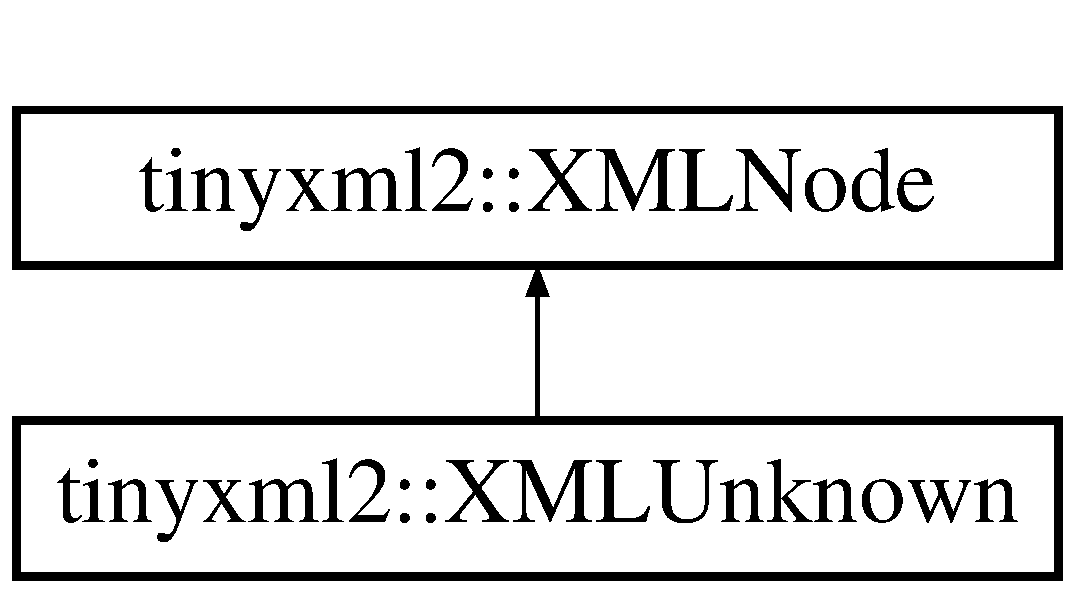
\includegraphics[height=2.000000cm]{classtinyxml2_1_1_x_m_l_unknown}
\end{center}
\end{figure}
\subsection*{Public Member Functions}
\begin{DoxyCompactItemize}
\item 
\mbox{\Hypertarget{classtinyxml2_1_1_x_m_l_unknown_af4374856421921cad578c8affae872b6}\label{classtinyxml2_1_1_x_m_l_unknown_af4374856421921cad578c8affae872b6}} 
virtual \mbox{\hyperlink{classtinyxml2_1_1_x_m_l_unknown}{X\+M\+L\+Unknown}} $\ast$ \mbox{\hyperlink{classtinyxml2_1_1_x_m_l_unknown_af4374856421921cad578c8affae872b6}{To\+Unknown}} ()
\begin{DoxyCompactList}\small\item\em Safely cast to an Unknown, or null. \end{DoxyCompactList}\item 
\mbox{\Hypertarget{classtinyxml2_1_1_x_m_l_unknown_a61b342b4f295cded1dc2f4402e97f07e}\label{classtinyxml2_1_1_x_m_l_unknown_a61b342b4f295cded1dc2f4402e97f07e}} 
virtual const \mbox{\hyperlink{classtinyxml2_1_1_x_m_l_unknown}{X\+M\+L\+Unknown}} $\ast$ {\bfseries To\+Unknown} () const
\item 
virtual bool \mbox{\hyperlink{classtinyxml2_1_1_x_m_l_unknown_a8a06b8c82117ca969a432e17a46830fc}{Accept}} (\mbox{\hyperlink{classtinyxml2_1_1_x_m_l_visitor}{X\+M\+L\+Visitor}} $\ast$visitor) const
\item 
virtual \mbox{\hyperlink{classtinyxml2_1_1_x_m_l_node}{X\+M\+L\+Node}} $\ast$ \mbox{\hyperlink{classtinyxml2_1_1_x_m_l_unknown_ab73b48b819aa4b2ef3815dc2d7d20d5f}{Shallow\+Clone}} (\mbox{\hyperlink{classtinyxml2_1_1_x_m_l_document}{X\+M\+L\+Document}} $\ast$document) const
\item 
virtual bool \mbox{\hyperlink{classtinyxml2_1_1_x_m_l_unknown_ac46767cd721d666e690a6231dfb618d1}{Shallow\+Equal}} (const \mbox{\hyperlink{classtinyxml2_1_1_x_m_l_node}{X\+M\+L\+Node}} $\ast$compare) const
\end{DoxyCompactItemize}
\subsection*{Protected Member Functions}
\begin{DoxyCompactItemize}
\item 
\mbox{\Hypertarget{classtinyxml2_1_1_x_m_l_unknown_a9391eb679598d50baba424e6f1aa367b}\label{classtinyxml2_1_1_x_m_l_unknown_a9391eb679598d50baba424e6f1aa367b}} 
{\bfseries X\+M\+L\+Unknown} (\mbox{\hyperlink{classtinyxml2_1_1_x_m_l_document}{X\+M\+L\+Document}} $\ast$doc)
\item 
\mbox{\Hypertarget{classtinyxml2_1_1_x_m_l_unknown_aefc332cc1e6e25736f364d1e5eeb31fe}\label{classtinyxml2_1_1_x_m_l_unknown_aefc332cc1e6e25736f364d1e5eeb31fe}} 
char $\ast$ {\bfseries Parse\+Deep} (char $\ast$p, \mbox{\hyperlink{classtinyxml2_1_1_str_pair}{Str\+Pair}} $\ast$parent\+End\+Tag, int $\ast$cur\+Line\+Num\+Ptr)
\end{DoxyCompactItemize}
\subsection*{Friends}
\begin{DoxyCompactItemize}
\item 
\mbox{\Hypertarget{classtinyxml2_1_1_x_m_l_unknown_a4eee3bda60c60a30e4e8cd4ea91c4c6e}\label{classtinyxml2_1_1_x_m_l_unknown_a4eee3bda60c60a30e4e8cd4ea91c4c6e}} 
class {\bfseries X\+M\+L\+Document}
\end{DoxyCompactItemize}
\subsection*{Additional Inherited Members}


\subsection{Detailed Description}
Any tag that Tiny\+X\+M\+L-\/2 doesn\textquotesingle{}t recognize is saved as an unknown. It is a tag of text, but should not be modified. It will be written back to the X\+ML, unchanged, when the file is saved.

D\+TD tags get thrown into X\+M\+L\+Unknowns. 

\subsection{Member Function Documentation}
\mbox{\Hypertarget{classtinyxml2_1_1_x_m_l_unknown_a8a06b8c82117ca969a432e17a46830fc}\label{classtinyxml2_1_1_x_m_l_unknown_a8a06b8c82117ca969a432e17a46830fc}} 
\index{tinyxml2\+::\+X\+M\+L\+Unknown@{tinyxml2\+::\+X\+M\+L\+Unknown}!Accept@{Accept}}
\index{Accept@{Accept}!tinyxml2\+::\+X\+M\+L\+Unknown@{tinyxml2\+::\+X\+M\+L\+Unknown}}
\subsubsection{\texorpdfstring{Accept()}{Accept()}}
{\footnotesize\ttfamily bool tinyxml2\+::\+X\+M\+L\+Unknown\+::\+Accept (\begin{DoxyParamCaption}\item[{\mbox{\hyperlink{classtinyxml2_1_1_x_m_l_visitor}{X\+M\+L\+Visitor}} $\ast$}]{visitor }\end{DoxyParamCaption}) const\hspace{0.3cm}{\ttfamily [virtual]}}

Accept a hierarchical visit of the nodes in the Tiny\+X\+M\+L-\/2 D\+OM. Every node in the X\+ML tree will be conditionally visited and the host will be called back via the \mbox{\hyperlink{classtinyxml2_1_1_x_m_l_visitor}{X\+M\+L\+Visitor}} interface.

This is essentially a S\+AX interface for Tiny\+X\+M\+L-\/2. (Note however it doesn\textquotesingle{}t re-\/parse the X\+ML for the callbacks, so the performance of Tiny\+X\+M\+L-\/2 is unchanged by using this interface versus any other.)

The interface has been based on ideas from\+:


\begin{DoxyItemize}
\item \href{http://www.saxproject.org/}{\tt http\+://www.\+saxproject.\+org/}
\item \href{http://c2.com/cgi/wiki?HierarchicalVisitorPattern}{\tt http\+://c2.\+com/cgi/wiki?\+Hierarchical\+Visitor\+Pattern}
\end{DoxyItemize}

Which are both good references for \char`\"{}visiting\char`\"{}.

An example of using \mbox{\hyperlink{classtinyxml2_1_1_x_m_l_unknown_a8a06b8c82117ca969a432e17a46830fc}{Accept()}}\+: \begin{DoxyVerb}XMLPrinter printer;
tinyxmlDoc.Accept( &printer );
const char* xmlcstr = printer.CStr();
\end{DoxyVerb}
 

Implements \mbox{\hyperlink{classtinyxml2_1_1_x_m_l_node_a81e66df0a44c67a7af17f3b77a152785}{tinyxml2\+::\+X\+M\+L\+Node}}.

\mbox{\Hypertarget{classtinyxml2_1_1_x_m_l_unknown_ab73b48b819aa4b2ef3815dc2d7d20d5f}\label{classtinyxml2_1_1_x_m_l_unknown_ab73b48b819aa4b2ef3815dc2d7d20d5f}} 
\index{tinyxml2\+::\+X\+M\+L\+Unknown@{tinyxml2\+::\+X\+M\+L\+Unknown}!Shallow\+Clone@{Shallow\+Clone}}
\index{Shallow\+Clone@{Shallow\+Clone}!tinyxml2\+::\+X\+M\+L\+Unknown@{tinyxml2\+::\+X\+M\+L\+Unknown}}
\subsubsection{\texorpdfstring{Shallow\+Clone()}{ShallowClone()}}
{\footnotesize\ttfamily \mbox{\hyperlink{classtinyxml2_1_1_x_m_l_node}{X\+M\+L\+Node}} $\ast$ tinyxml2\+::\+X\+M\+L\+Unknown\+::\+Shallow\+Clone (\begin{DoxyParamCaption}\item[{\mbox{\hyperlink{classtinyxml2_1_1_x_m_l_document}{X\+M\+L\+Document}} $\ast$}]{document }\end{DoxyParamCaption}) const\hspace{0.3cm}{\ttfamily [virtual]}}

Make a copy of this node, but not its children. You may pass in a Document pointer that will be the owner of the new Node. If the \textquotesingle{}document\textquotesingle{} is null, then the node returned will be allocated from the current Document. (this-\/$>$\mbox{\hyperlink{classtinyxml2_1_1_x_m_l_node_af343d1ef0b45c0020e62d784d7e67a68}{Get\+Document()}})

Note\+: if called on a \mbox{\hyperlink{classtinyxml2_1_1_x_m_l_document}{X\+M\+L\+Document}}, this will return null. 

Implements \mbox{\hyperlink{classtinyxml2_1_1_x_m_l_node_a8402cbd3129d20e9e6024bbcc0531283}{tinyxml2\+::\+X\+M\+L\+Node}}.

\mbox{\Hypertarget{classtinyxml2_1_1_x_m_l_unknown_ac46767cd721d666e690a6231dfb618d1}\label{classtinyxml2_1_1_x_m_l_unknown_ac46767cd721d666e690a6231dfb618d1}} 
\index{tinyxml2\+::\+X\+M\+L\+Unknown@{tinyxml2\+::\+X\+M\+L\+Unknown}!Shallow\+Equal@{Shallow\+Equal}}
\index{Shallow\+Equal@{Shallow\+Equal}!tinyxml2\+::\+X\+M\+L\+Unknown@{tinyxml2\+::\+X\+M\+L\+Unknown}}
\subsubsection{\texorpdfstring{Shallow\+Equal()}{ShallowEqual()}}
{\footnotesize\ttfamily bool tinyxml2\+::\+X\+M\+L\+Unknown\+::\+Shallow\+Equal (\begin{DoxyParamCaption}\item[{const \mbox{\hyperlink{classtinyxml2_1_1_x_m_l_node}{X\+M\+L\+Node}} $\ast$}]{compare }\end{DoxyParamCaption}) const\hspace{0.3cm}{\ttfamily [virtual]}}

Test if 2 nodes are the same, but don\textquotesingle{}t test children. The 2 nodes do not need to be in the same Document.

Note\+: if called on a \mbox{\hyperlink{classtinyxml2_1_1_x_m_l_document}{X\+M\+L\+Document}}, this will return false. 

Implements \mbox{\hyperlink{classtinyxml2_1_1_x_m_l_node_a7ce18b751c3ea09eac292dca264f9226}{tinyxml2\+::\+X\+M\+L\+Node}}.



The documentation for this class was generated from the following files\+:\begin{DoxyCompactItemize}
\item 
Source/\+Utils/tinyxml2.\+h\item 
Source/\+Utils/tinyxml2.\+cpp\end{DoxyCompactItemize}

\hypertarget{classtinyxml2_1_1_x_m_l_util}{}\section{tinyxml2\+:\+:X\+M\+L\+Util Class Reference}
\label{classtinyxml2_1_1_x_m_l_util}\index{tinyxml2\+::\+X\+M\+L\+Util@{tinyxml2\+::\+X\+M\+L\+Util}}
\subsection*{Static Public Member Functions}
\begin{DoxyCompactItemize}
\item 
\mbox{\Hypertarget{classtinyxml2_1_1_x_m_l_util_ab626a194b3523a5ba8b9dbaa2a165202}\label{classtinyxml2_1_1_x_m_l_util_ab626a194b3523a5ba8b9dbaa2a165202}} 
static const char $\ast$ {\bfseries Skip\+White\+Space} (const char $\ast$p, int $\ast$cur\+Line\+Num\+Ptr)
\item 
\mbox{\Hypertarget{classtinyxml2_1_1_x_m_l_util_abb6cb3e71f88efca82cb7157367fd91e}\label{classtinyxml2_1_1_x_m_l_util_abb6cb3e71f88efca82cb7157367fd91e}} 
static char $\ast$ {\bfseries Skip\+White\+Space} (char $\ast$p, int $\ast$cur\+Line\+Num\+Ptr)
\item 
\mbox{\Hypertarget{classtinyxml2_1_1_x_m_l_util_a357ec3af8fc433d19023a815f45e8e33}\label{classtinyxml2_1_1_x_m_l_util_a357ec3af8fc433d19023a815f45e8e33}} 
static bool {\bfseries Is\+White\+Space} (char p)
\item 
\mbox{\Hypertarget{classtinyxml2_1_1_x_m_l_util_abe106a69ac4d942a4381a4d9dfd0e0bd}\label{classtinyxml2_1_1_x_m_l_util_abe106a69ac4d942a4381a4d9dfd0e0bd}} 
static bool {\bfseries Is\+Name\+Start\+Char} (unsigned char ch)
\item 
\mbox{\Hypertarget{classtinyxml2_1_1_x_m_l_util_a04b17341538fa11752f24b4301d19485}\label{classtinyxml2_1_1_x_m_l_util_a04b17341538fa11752f24b4301d19485}} 
static bool {\bfseries Is\+Name\+Char} (unsigned char ch)
\item 
\mbox{\Hypertarget{classtinyxml2_1_1_x_m_l_util_acfcd287cacfd2533e1bc9ea4dfb56602}\label{classtinyxml2_1_1_x_m_l_util_acfcd287cacfd2533e1bc9ea4dfb56602}} 
static bool {\bfseries String\+Equal} (const char $\ast$p, const char $\ast$q, int n\+Char=I\+N\+T\+\_\+\+M\+AX)
\item 
\mbox{\Hypertarget{classtinyxml2_1_1_x_m_l_util_ad7fd82e0fe610d73ef7bf9f359f104a3}\label{classtinyxml2_1_1_x_m_l_util_ad7fd82e0fe610d73ef7bf9f359f104a3}} 
static bool {\bfseries Is\+U\+T\+F8\+Continuation} (char p)
\item 
\mbox{\Hypertarget{classtinyxml2_1_1_x_m_l_util_ae9bcb2bc3cd6475fdc644c8c17790555}\label{classtinyxml2_1_1_x_m_l_util_ae9bcb2bc3cd6475fdc644c8c17790555}} 
static const char $\ast$ {\bfseries Read\+B\+OM} (const char $\ast$p, bool $\ast$has\+B\+OM)
\item 
\mbox{\Hypertarget{classtinyxml2_1_1_x_m_l_util_a5a96e5144a8d693dc4bcd783d9964648}\label{classtinyxml2_1_1_x_m_l_util_a5a96e5144a8d693dc4bcd783d9964648}} 
static const char $\ast$ {\bfseries Get\+Character\+Ref} (const char $\ast$p, char $\ast$value, int $\ast$length)
\item 
\mbox{\Hypertarget{classtinyxml2_1_1_x_m_l_util_a31c00d5c5dfb38382de1dfcaf4be3595}\label{classtinyxml2_1_1_x_m_l_util_a31c00d5c5dfb38382de1dfcaf4be3595}} 
static void {\bfseries Convert\+U\+T\+F32\+To\+U\+T\+F8} (unsigned long input, char $\ast$output, int $\ast$length)
\item 
\mbox{\Hypertarget{classtinyxml2_1_1_x_m_l_util_a3cd6c703d49b9d51bdf0f4ff6aa021c7}\label{classtinyxml2_1_1_x_m_l_util_a3cd6c703d49b9d51bdf0f4ff6aa021c7}} 
static void {\bfseries To\+Str} (int v, char $\ast$buffer, int buffer\+Size)
\item 
\mbox{\Hypertarget{classtinyxml2_1_1_x_m_l_util_ac00c2e52c1c36dab3ff41d86a9bf60f9}\label{classtinyxml2_1_1_x_m_l_util_ac00c2e52c1c36dab3ff41d86a9bf60f9}} 
static void {\bfseries To\+Str} (unsigned v, char $\ast$buffer, int buffer\+Size)
\item 
\mbox{\Hypertarget{classtinyxml2_1_1_x_m_l_util_adba0718527ae9e80f663a71ea325cb11}\label{classtinyxml2_1_1_x_m_l_util_adba0718527ae9e80f663a71ea325cb11}} 
static void {\bfseries To\+Str} (bool v, char $\ast$buffer, int buffer\+Size)
\item 
\mbox{\Hypertarget{classtinyxml2_1_1_x_m_l_util_a8957ad44fee5fa02ba52d73aad4d0a31}\label{classtinyxml2_1_1_x_m_l_util_a8957ad44fee5fa02ba52d73aad4d0a31}} 
static void {\bfseries To\+Str} (float v, char $\ast$buffer, int buffer\+Size)
\item 
\mbox{\Hypertarget{classtinyxml2_1_1_x_m_l_util_a1cd141e50980fcddd6bf9af5de4b1db7}\label{classtinyxml2_1_1_x_m_l_util_a1cd141e50980fcddd6bf9af5de4b1db7}} 
static void {\bfseries To\+Str} (double v, char $\ast$buffer, int buffer\+Size)
\item 
\mbox{\Hypertarget{classtinyxml2_1_1_x_m_l_util_a26a8cb5b833ad587b3af39469c8111de}\label{classtinyxml2_1_1_x_m_l_util_a26a8cb5b833ad587b3af39469c8111de}} 
static void {\bfseries To\+Str} (int64\+\_\+t v, char $\ast$buffer, int buffer\+Size)
\item 
\mbox{\Hypertarget{classtinyxml2_1_1_x_m_l_util_ad4df4023d11ee3fca9689c49b9707323}\label{classtinyxml2_1_1_x_m_l_util_ad4df4023d11ee3fca9689c49b9707323}} 
static bool {\bfseries To\+Int} (const char $\ast$str, int $\ast$value)
\item 
\mbox{\Hypertarget{classtinyxml2_1_1_x_m_l_util_a210c8637d5eb4ce3d4625294af0efc2f}\label{classtinyxml2_1_1_x_m_l_util_a210c8637d5eb4ce3d4625294af0efc2f}} 
static bool {\bfseries To\+Unsigned} (const char $\ast$str, unsigned $\ast$value)
\item 
\mbox{\Hypertarget{classtinyxml2_1_1_x_m_l_util_ae5b03e0a1ca5d42052a7ac540f7aa12a}\label{classtinyxml2_1_1_x_m_l_util_ae5b03e0a1ca5d42052a7ac540f7aa12a}} 
static bool {\bfseries To\+Bool} (const char $\ast$str, bool $\ast$value)
\item 
\mbox{\Hypertarget{classtinyxml2_1_1_x_m_l_util_a399e71edb5f29d61ea81d91ee0332bb9}\label{classtinyxml2_1_1_x_m_l_util_a399e71edb5f29d61ea81d91ee0332bb9}} 
static bool {\bfseries To\+Float} (const char $\ast$str, float $\ast$value)
\item 
\mbox{\Hypertarget{classtinyxml2_1_1_x_m_l_util_ad8f75ac140fb19c1c6e164a957c4cd53}\label{classtinyxml2_1_1_x_m_l_util_ad8f75ac140fb19c1c6e164a957c4cd53}} 
static bool {\bfseries To\+Double} (const char $\ast$str, double $\ast$value)
\item 
\mbox{\Hypertarget{classtinyxml2_1_1_x_m_l_util_afe2ea09257431cd2b4b6d440552e4195}\label{classtinyxml2_1_1_x_m_l_util_afe2ea09257431cd2b4b6d440552e4195}} 
static bool {\bfseries To\+Int64} (const char $\ast$str, int64\+\_\+t $\ast$value)
\item 
\mbox{\Hypertarget{classtinyxml2_1_1_x_m_l_util_af98a6a80dbeec4679366c1aba4c5b747}\label{classtinyxml2_1_1_x_m_l_util_af98a6a80dbeec4679366c1aba4c5b747}} 
static void {\bfseries Set\+Bool\+Serialization} (const char $\ast$write\+True, const char $\ast$write\+False)
\end{DoxyCompactItemize}


The documentation for this class was generated from the following files\+:\begin{DoxyCompactItemize}
\item 
Source/\+Utils/tinyxml2.\+h\item 
Source/\+Utils/tinyxml2.\+cpp\end{DoxyCompactItemize}

\hypertarget{classtinyxml2_1_1_x_m_l_visitor}{}\section{tinyxml2\+:\+:X\+M\+L\+Visitor Class Reference}
\label{classtinyxml2_1_1_x_m_l_visitor}\index{tinyxml2\+::\+X\+M\+L\+Visitor@{tinyxml2\+::\+X\+M\+L\+Visitor}}


{\ttfamily \#include $<$tinyxml2.\+h$>$}

Inheritance diagram for tinyxml2\+:\+:X\+M\+L\+Visitor\+:\begin{figure}[H]
\begin{center}
\leavevmode
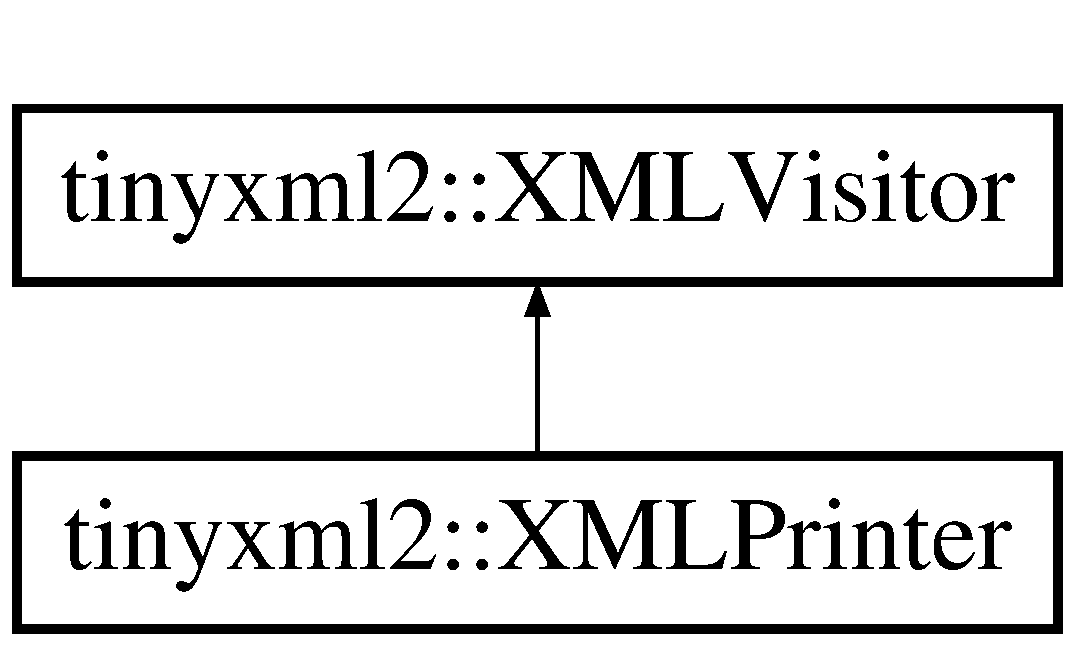
\includegraphics[height=2.000000cm]{classtinyxml2_1_1_x_m_l_visitor}
\end{center}
\end{figure}
\subsection*{Public Member Functions}
\begin{DoxyCompactItemize}
\item 
\mbox{\Hypertarget{classtinyxml2_1_1_x_m_l_visitor_acb3c22fc5f60eb9db98f533f2761f67d}\label{classtinyxml2_1_1_x_m_l_visitor_acb3c22fc5f60eb9db98f533f2761f67d}} 
virtual bool \mbox{\hyperlink{classtinyxml2_1_1_x_m_l_visitor_acb3c22fc5f60eb9db98f533f2761f67d}{Visit\+Enter}} (const \mbox{\hyperlink{classtinyxml2_1_1_x_m_l_document}{X\+M\+L\+Document}} \&)
\begin{DoxyCompactList}\small\item\em Visit a document. \end{DoxyCompactList}\item 
\mbox{\Hypertarget{classtinyxml2_1_1_x_m_l_visitor_a170e9989cd046ba904f302d087e07086}\label{classtinyxml2_1_1_x_m_l_visitor_a170e9989cd046ba904f302d087e07086}} 
virtual bool \mbox{\hyperlink{classtinyxml2_1_1_x_m_l_visitor_a170e9989cd046ba904f302d087e07086}{Visit\+Exit}} (const \mbox{\hyperlink{classtinyxml2_1_1_x_m_l_document}{X\+M\+L\+Document}} \&)
\begin{DoxyCompactList}\small\item\em Visit a document. \end{DoxyCompactList}\item 
\mbox{\Hypertarget{classtinyxml2_1_1_x_m_l_visitor_af97980a17dd4e37448b181f5ddfa92b5}\label{classtinyxml2_1_1_x_m_l_visitor_af97980a17dd4e37448b181f5ddfa92b5}} 
virtual bool \mbox{\hyperlink{classtinyxml2_1_1_x_m_l_visitor_af97980a17dd4e37448b181f5ddfa92b5}{Visit\+Enter}} (const \mbox{\hyperlink{classtinyxml2_1_1_x_m_l_element}{X\+M\+L\+Element}} \&, const \mbox{\hyperlink{classtinyxml2_1_1_x_m_l_attribute}{X\+M\+L\+Attribute}} $\ast$)
\begin{DoxyCompactList}\small\item\em Visit an element. \end{DoxyCompactList}\item 
\mbox{\Hypertarget{classtinyxml2_1_1_x_m_l_visitor_a772f10ddc83f881956d32628faa16eb6}\label{classtinyxml2_1_1_x_m_l_visitor_a772f10ddc83f881956d32628faa16eb6}} 
virtual bool \mbox{\hyperlink{classtinyxml2_1_1_x_m_l_visitor_a772f10ddc83f881956d32628faa16eb6}{Visit\+Exit}} (const \mbox{\hyperlink{classtinyxml2_1_1_x_m_l_element}{X\+M\+L\+Element}} \&)
\begin{DoxyCompactList}\small\item\em Visit an element. \end{DoxyCompactList}\item 
\mbox{\Hypertarget{classtinyxml2_1_1_x_m_l_visitor_adc75bd459fc7ba8223b50f0616767f9a}\label{classtinyxml2_1_1_x_m_l_visitor_adc75bd459fc7ba8223b50f0616767f9a}} 
virtual bool \mbox{\hyperlink{classtinyxml2_1_1_x_m_l_visitor_adc75bd459fc7ba8223b50f0616767f9a}{Visit}} (const \mbox{\hyperlink{classtinyxml2_1_1_x_m_l_declaration}{X\+M\+L\+Declaration}} \&)
\begin{DoxyCompactList}\small\item\em Visit a declaration. \end{DoxyCompactList}\item 
\mbox{\Hypertarget{classtinyxml2_1_1_x_m_l_visitor_af30233565856480ea48b6fa0d6dec65b}\label{classtinyxml2_1_1_x_m_l_visitor_af30233565856480ea48b6fa0d6dec65b}} 
virtual bool \mbox{\hyperlink{classtinyxml2_1_1_x_m_l_visitor_af30233565856480ea48b6fa0d6dec65b}{Visit}} (const \mbox{\hyperlink{classtinyxml2_1_1_x_m_l_text}{X\+M\+L\+Text}} \&)
\begin{DoxyCompactList}\small\item\em Visit a text node. \end{DoxyCompactList}\item 
\mbox{\Hypertarget{classtinyxml2_1_1_x_m_l_visitor_acc8147fb5a85f6c65721654e427752d7}\label{classtinyxml2_1_1_x_m_l_visitor_acc8147fb5a85f6c65721654e427752d7}} 
virtual bool \mbox{\hyperlink{classtinyxml2_1_1_x_m_l_visitor_acc8147fb5a85f6c65721654e427752d7}{Visit}} (const \mbox{\hyperlink{classtinyxml2_1_1_x_m_l_comment}{X\+M\+L\+Comment}} \&)
\begin{DoxyCompactList}\small\item\em Visit a comment node. \end{DoxyCompactList}\item 
\mbox{\Hypertarget{classtinyxml2_1_1_x_m_l_visitor_a14e4748387c34bf53d24e8119bb1f292}\label{classtinyxml2_1_1_x_m_l_visitor_a14e4748387c34bf53d24e8119bb1f292}} 
virtual bool \mbox{\hyperlink{classtinyxml2_1_1_x_m_l_visitor_a14e4748387c34bf53d24e8119bb1f292}{Visit}} (const \mbox{\hyperlink{classtinyxml2_1_1_x_m_l_unknown}{X\+M\+L\+Unknown}} \&)
\begin{DoxyCompactList}\small\item\em Visit an unknown node. \end{DoxyCompactList}\end{DoxyCompactItemize}


\subsection{Detailed Description}
Implements the interface to the \char`\"{}\+Visitor pattern\char`\"{} (see the Accept() method.) If you call the Accept() method, it requires being passed a \mbox{\hyperlink{classtinyxml2_1_1_x_m_l_visitor}{X\+M\+L\+Visitor}} class to handle callbacks. For nodes that contain other nodes (Document, Element) you will get called with a Visit\+Enter/\+Visit\+Exit pair. Nodes that are always leafs are simply called with \mbox{\hyperlink{classtinyxml2_1_1_x_m_l_visitor_adc75bd459fc7ba8223b50f0616767f9a}{Visit()}}.

If you return \textquotesingle{}true\textquotesingle{} from a Visit method, recursive parsing will continue. If you return false, {\bfseries no children of this node or its siblings} will be visited.

All flavors of Visit methods have a default implementation that returns \textquotesingle{}true\textquotesingle{} (continue visiting). You need to only override methods that are interesting to you.

Generally Accept() is called on the \mbox{\hyperlink{classtinyxml2_1_1_x_m_l_document}{X\+M\+L\+Document}}, although all nodes support visiting.

You should never change the document from a callback.

\begin{DoxySeeAlso}{See also}
\mbox{\hyperlink{classtinyxml2_1_1_x_m_l_node_a81e66df0a44c67a7af17f3b77a152785}{X\+M\+L\+Node\+::\+Accept()}} 
\end{DoxySeeAlso}


The documentation for this class was generated from the following file\+:\begin{DoxyCompactItemize}
\item 
Source/\+Utils/tinyxml2.\+h\end{DoxyCompactItemize}

\chapter{File Documentation}
\hypertarget{_application_8h}{}\section{Source/\+Application/\+Application.h File Reference}
\label{_application_8h}\index{Source/\+Application/\+Application.\+h@{Source/\+Application/\+Application.\+h}}
{\ttfamily \#include \char`\"{}../\+Logic/\+Game.\+h\char`\"{}}\newline
{\ttfamily \#include \char`\"{}../\+Views/\+View.\+h\char`\"{}}\newline
{\ttfamily \#include \char`\"{}../\+Logic/\+Input/\+Input\+System.\+h\char`\"{}}\newline
{\ttfamily \#include \char`\"{}../\+Utils/\+Macros.\+h\char`\"{}}\newline
{\ttfamily \#include $<$string$>$}\newline
\subsection*{Classes}
\begin{DoxyCompactItemize}
\item 
class \mbox{\hyperlink{class_application}{Application}}
\begin{DoxyCompactList}\small\item\em Engine entry point. \end{DoxyCompactList}\end{DoxyCompactItemize}

\hypertarget{_event_system_8h}{}\section{Source/\+Logic/\+Events/\+Event\+System.h File Reference}
\label{_event_system_8h}\index{Source/\+Logic/\+Events/\+Event\+System.\+h@{Source/\+Logic/\+Events/\+Event\+System.\+h}}
{\ttfamily \#include $<$map$>$}\newline
{\ttfamily \#include $<$vector$>$}\newline
{\ttfamily \#include $<$S\+D\+L\+\_\+rect.\+h$>$}\newline
\subsection*{Classes}
\begin{DoxyCompactItemize}
\item 
struct \mbox{\hyperlink{struct_event}{Event}}
\begin{DoxyCompactList}\small\item\em \mbox{\hyperlink{struct_event}{Event}} structure. \end{DoxyCompactList}\item 
struct \mbox{\hyperlink{struct_game_event}{Game\+Event}}
\begin{DoxyCompactList}\small\item\em Structure for \mbox{\hyperlink{class_game}{Game}} Logic Events. \end{DoxyCompactList}\item 
struct \mbox{\hyperlink{struct_map_event}{Map\+Event}}
\begin{DoxyCompactList}\small\item\em Structure for Map System Events. \end{DoxyCompactList}\item 
struct \mbox{\hyperlink{struct_sfx_event}{Sfx\+Event}}
\begin{DoxyCompactList}\small\item\em Structure for Sfx Events. \end{DoxyCompactList}\item 
struct \mbox{\hyperlink{struct_music_event}{Music\+Event}}
\begin{DoxyCompactList}\small\item\em Structure for Music Events. \end{DoxyCompactList}\item 
struct \mbox{\hyperlink{struct_texture_event}{Texture\+Event}}
\begin{DoxyCompactList}\small\item\em Structure for Texture events. \end{DoxyCompactList}\item 
class \mbox{\hyperlink{class_i_event_handler}{I\+Event\+Handler}}
\begin{DoxyCompactList}\small\item\em Interface for \mbox{\hyperlink{struct_event}{Event}} handlers. \end{DoxyCompactList}\item 
class \mbox{\hyperlink{class_event_system}{Event\+System}}
\begin{DoxyCompactList}\small\item\em System to handle sending and recieving of Events. \end{DoxyCompactList}\end{DoxyCompactItemize}
\subsection*{Typedefs}
\begin{DoxyCompactItemize}
\item 
\mbox{\Hypertarget{_event_system_8h_a1952a96deec9bc6042cb51af3e68f4ca}\label{_event_system_8h_a1952a96deec9bc6042cb51af3e68f4ca}} 
typedef std\+::vector$<$ \mbox{\hyperlink{class_i_event_handler}{I\+Event\+Handler}} $\ast$ $>$ {\bfseries Event\+Handlers}
\end{DoxyCompactItemize}

\hypertarget{_game_8h}{}\section{Source/\+Logic/\+Game.h File Reference}
\label{_game_8h}\index{Source/\+Logic/\+Game.\+h@{Source/\+Logic/\+Game.\+h}}
{\ttfamily \#include \char`\"{}I\+Updatable.\+h\char`\"{}}\newline
{\ttfamily \#include \char`\"{}../\+Views/\+I\+Renderable.\+h\char`\"{}}\newline
{\ttfamily \#include \char`\"{}../\+Utils/\+Macros.\+h\char`\"{}}\newline
{\ttfamily \#include \char`\"{}Game\+Objects\textbackslash{}\+Game\+Object.\+h\char`\"{}}\newline
{\ttfamily \#include $<$vector$>$}\newline
{\ttfamily \#include \char`\"{}Events/\+Event\+System.\+h\char`\"{}}\newline
\subsection*{Classes}
\begin{DoxyCompactItemize}
\item 
class \mbox{\hyperlink{class_game}{Game}}
\begin{DoxyCompactList}\small\item\em Represents game logic. \end{DoxyCompactList}\end{DoxyCompactItemize}

\hypertarget{_component_pool_8h}{}\section{Source/\+Logic/\+Game\+Objects/\+Component\+Pool.h File Reference}
\label{_component_pool_8h}\index{Source/\+Logic/\+Game\+Objects/\+Component\+Pool.\+h@{Source/\+Logic/\+Game\+Objects/\+Component\+Pool.\+h}}
{\ttfamily \#include $<$memory$>$}\newline
{\ttfamily \#include $<$unordered\+\_\+map$>$}\newline
\subsection*{Classes}
\begin{DoxyCompactItemize}
\item 
class \mbox{\hyperlink{class_component_pool}{Component\+Pool}}
\begin{DoxyCompactList}\small\item\em Pool of I\+Components. \end{DoxyCompactList}\end{DoxyCompactItemize}
\subsection*{Typedefs}
\begin{DoxyCompactItemize}
\item 
\mbox{\Hypertarget{_component_pool_8h_a8b8bf5d1204ced799bda98b0fe7ab84e}\label{_component_pool_8h_a8b8bf5d1204ced799bda98b0fe7ab84e}} 
typedef std\+::shared\+\_\+ptr$<$ \mbox{\hyperlink{class_i_component}{I\+Component}} $>$ {\bfseries Component\+Ptr}
\end{DoxyCompactItemize}

\hypertarget{_game_object_8h}{}\section{Source/\+Logic/\+Game\+Objects/\+Game\+Object.h File Reference}
\label{_game_object_8h}\index{Source/\+Logic/\+Game\+Objects/\+Game\+Object.\+h@{Source/\+Logic/\+Game\+Objects/\+Game\+Object.\+h}}
{\ttfamily \#include \char`\"{}../\+I\+Updatable.\+h\char`\"{}}\newline
{\ttfamily \#include \char`\"{}../../\+Views/\+I\+Renderable.\+h\char`\"{}}\newline
{\ttfamily \#include \char`\"{}../\+Math/\+Vector2\+D.\+h\char`\"{}}\newline
{\ttfamily \#include $<$string$>$}\newline
{\ttfamily \#include $<$S\+D\+L\+\_\+rect.\+h$>$}\newline
{\ttfamily \#include \char`\"{}../../\+Utils/\+Macros.\+h\char`\"{}}\newline
{\ttfamily \#include $<$unordered\+\_\+map$>$}\newline
{\ttfamily \#include \char`\"{}Component\+Pool.\+h\char`\"{}}\newline
\subsection*{Classes}
\begin{DoxyCompactItemize}
\item 
class \mbox{\hyperlink{class_game_object}{Game\+Object}}
\begin{DoxyCompactList}\small\item\em Represents a game object. \end{DoxyCompactList}\end{DoxyCompactItemize}

\hypertarget{_i_component_8h}{}\section{Source/\+Logic/\+Game\+Objects/\+I\+Component.h File Reference}
\label{_i_component_8h}\index{Source/\+Logic/\+Game\+Objects/\+I\+Component.\+h@{Source/\+Logic/\+Game\+Objects/\+I\+Component.\+h}}
\subsection*{Classes}
\begin{DoxyCompactItemize}
\item 
class \mbox{\hyperlink{class_i_component}{I\+Component}}
\begin{DoxyCompactList}\small\item\em Interface for Components. \end{DoxyCompactList}\end{DoxyCompactItemize}

\hypertarget{_movement_component_8h}{}\section{Source/\+Logic/\+Game\+Objects/\+Movement\+Component.h File Reference}
\label{_movement_component_8h}\index{Source/\+Logic/\+Game\+Objects/\+Movement\+Component.\+h@{Source/\+Logic/\+Game\+Objects/\+Movement\+Component.\+h}}
{\ttfamily \#include \char`\"{}I\+Component.\+h\char`\"{}}\newline
{\ttfamily \#include \char`\"{}../\+Math/\+Vector2\+D.\+h\char`\"{}}\newline
{\ttfamily \#include \char`\"{}../\+I\+Updatable.\+h\char`\"{}}\newline
\subsection*{Classes}
\begin{DoxyCompactItemize}
\item 
class \mbox{\hyperlink{class_movement_component}{Movement\+Component}}
\begin{DoxyCompactList}\small\item\em Component to hold and handle movement data. \end{DoxyCompactList}\end{DoxyCompactItemize}

\hypertarget{_physics_component_8h}{}\section{Source/\+Logic/\+Game\+Objects/\+Physics\+Component.h File Reference}
\label{_physics_component_8h}\index{Source/\+Logic/\+Game\+Objects/\+Physics\+Component.\+h@{Source/\+Logic/\+Game\+Objects/\+Physics\+Component.\+h}}
{\ttfamily \#include \char`\"{}I\+Component.\+h\char`\"{}}\newline
{\ttfamily \#include \char`\"{}../\+Physics/\+Physics\+System.\+h\char`\"{}}\newline
\subsection*{Classes}
\begin{DoxyCompactItemize}
\item 
class \mbox{\hyperlink{struct_physics_component}{Physics\+Component}}
\begin{DoxyCompactList}\small\item\em Component that enables physics. \end{DoxyCompactList}\end{DoxyCompactItemize}

\hypertarget{_texture_component_8h}{}\section{Source/\+Logic/\+Game\+Objects/\+Texture\+Component.h File Reference}
\label{_texture_component_8h}\index{Source/\+Logic/\+Game\+Objects/\+Texture\+Component.\+h@{Source/\+Logic/\+Game\+Objects/\+Texture\+Component.\+h}}
{\ttfamily \#include \char`\"{}I\+Component.\+h\char`\"{}}\newline
{\ttfamily \#include $<$string$>$}\newline
{\ttfamily \#include $<$S\+D\+L\+\_\+rect.\+h$>$}\newline
\subsection*{Classes}
\begin{DoxyCompactItemize}
\item 
struct \mbox{\hyperlink{struct_texture_component}{Texture\+Component}}
\begin{DoxyCompactList}\small\item\em Structure to store texture data. \end{DoxyCompactList}\end{DoxyCompactItemize}

\hypertarget{_command_8h}{}\section{Source/\+Logic/\+Input/\+Command.h File Reference}
\label{_command_8h}\index{Source/\+Logic/\+Input/\+Command.\+h@{Source/\+Logic/\+Input/\+Command.\+h}}
\subsection*{Classes}
\begin{DoxyCompactItemize}
\item 
class \mbox{\hyperlink{class_command}{Command}}
\begin{DoxyCompactList}\small\item\em Interpreted input data and base class for Commands. \end{DoxyCompactList}\end{DoxyCompactItemize}

\hypertarget{_input_interpreter_8h}{}\section{Source/\+Logic/\+Input/\+Input\+Interpreter.h File Reference}
\label{_input_interpreter_8h}\index{Source/\+Logic/\+Input/\+Input\+Interpreter.\+h@{Source/\+Logic/\+Input/\+Input\+Interpreter.\+h}}
{\ttfamily \#include $<$map$>$}\newline
{\ttfamily \#include \char`\"{}Key\+Command.\+h\char`\"{}}\newline
\subsection*{Classes}
\begin{DoxyCompactItemize}
\item 
class \mbox{\hyperlink{class_input_interpreter}{Input\+Interpreter}}
\begin{DoxyCompactList}\small\item\em Interpretes user input into commands. \end{DoxyCompactList}\end{DoxyCompactItemize}
\subsection*{Typedefs}
\begin{DoxyCompactItemize}
\item 
\mbox{\Hypertarget{_input_interpreter_8h_aee1e837fad0ecb1de3909ce3654870cb}\label{_input_interpreter_8h_aee1e837fad0ecb1de3909ce3654870cb}} 
typedef int32\+\_\+t {\bfseries S\+D\+L\+\_\+\+Keycode}
\end{DoxyCompactItemize}

\hypertarget{_input_system_8h}{}\section{Source/\+Logic/\+Input/\+Input\+System.h File Reference}
\label{_input_system_8h}\index{Source/\+Logic/\+Input/\+Input\+System.\+h@{Source/\+Logic/\+Input/\+Input\+System.\+h}}
{\ttfamily \#include \char`\"{}Input\+Interpreter.\+h\char`\"{}}\newline
\subsection*{Classes}
\begin{DoxyCompactItemize}
\item 
class \mbox{\hyperlink{class_input_system}{Input\+System}}
\begin{DoxyCompactList}\small\item\em Handles sdl input events then, tells \mbox{\hyperlink{class_input_interpreter}{Input\+Interpreter}} to interpret, then sends the interpreted input to \mbox{\hyperlink{class_game}{Game}}. \end{DoxyCompactList}\end{DoxyCompactItemize}

\hypertarget{_key_command_8h}{}\section{Source/\+Logic/\+Input/\+Key\+Command.h File Reference}
\label{_key_command_8h}\index{Source/\+Logic/\+Input/\+Key\+Command.\+h@{Source/\+Logic/\+Input/\+Key\+Command.\+h}}
{\ttfamily \#include \char`\"{}Command.\+h\char`\"{}}\newline
{\ttfamily \#include $<$S\+D\+L\+\_\+keycode.\+h$>$}\newline
\subsection*{Classes}
\begin{DoxyCompactItemize}
\item 
class \mbox{\hyperlink{class_key_command}{Key\+Command}}
\begin{DoxyCompactList}\small\item\em Represents a keyboard command. \end{DoxyCompactList}\end{DoxyCompactItemize}

\hypertarget{_i_updatable_8h}{}\section{Source/\+Logic/\+I\+Updatable.h File Reference}
\label{_i_updatable_8h}\index{Source/\+Logic/\+I\+Updatable.\+h@{Source/\+Logic/\+I\+Updatable.\+h}}
\subsection*{Classes}
\begin{DoxyCompactItemize}
\item 
class \mbox{\hyperlink{class_i_updatable}{I\+Updatable}}
\begin{DoxyCompactList}\small\item\em Interface for anything that updates. \end{DoxyCompactList}\end{DoxyCompactItemize}

\hypertarget{_vector2_d_8h}{}\section{Source/\+Logic/\+Math/\+Vector2D.h File Reference}
\label{_vector2_d_8h}\index{Source/\+Logic/\+Math/\+Vector2\+D.\+h@{Source/\+Logic/\+Math/\+Vector2\+D.\+h}}
\subsection*{Classes}
\begin{DoxyCompactItemize}
\item 
struct \mbox{\hyperlink{struct_vector2_d}{Vector2D}}
\begin{DoxyCompactList}\small\item\em Represents 2D vectors in game space. \end{DoxyCompactList}\end{DoxyCompactItemize}

\hypertarget{_physics_system_8h}{}\section{Source/\+Logic/\+Physics/\+Physics\+System.h File Reference}
\label{_physics_system_8h}\index{Source/\+Logic/\+Physics/\+Physics\+System.\+h@{Source/\+Logic/\+Physics/\+Physics\+System.\+h}}
{\ttfamily \#include $<$Box2\+D.\+h$>$}\newline
{\ttfamily \#include $<$vector$>$}\newline
{\ttfamily \#include \char`\"{}../\+I\+Updatable.\+h\char`\"{}}\newline
{\ttfamily \#include \char`\"{}../\+Events/\+Event\+System.\+h\char`\"{}}\newline
\subsection*{Classes}
\begin{DoxyCompactItemize}
\item 
class \mbox{\hyperlink{class_physics_system}{Physics\+System}}
\begin{DoxyCompactList}\small\item\em Physics system for engine. \end{DoxyCompactList}\end{DoxyCompactItemize}

\hypertarget{_macros_8h}{}\section{Source/\+Utils/\+Macros.h File Reference}
\label{_macros_8h}\index{Source/\+Utils/\+Macros.\+h@{Source/\+Utils/\+Macros.\+h}}


Contains useful macros and other defines for engine use.  


\subsection*{Macros}
\begin{DoxyCompactItemize}
\item 
\mbox{\Hypertarget{_macros_8h_a9ce0e6835f82908079752fa4ebe70dc9}\label{_macros_8h_a9ce0e6835f82908079752fa4ebe70dc9}} 
\#define \mbox{\hyperlink{_macros_8h_a9ce0e6835f82908079752fa4ebe70dc9}{P\+H\+A\+Z\+E\+\_\+\+A\+PI}}~\+\_\+\+\_\+declspec(dllexport)
\begin{DoxyCompactList}\small\item\em Exports a function for game use. \end{DoxyCompactList}\item 
\mbox{\Hypertarget{_macros_8h_a011f7e48a812611f072ec1e8dffe1fa1}\label{_macros_8h_a011f7e48a812611f072ec1e8dffe1fa1}} 
\#define \mbox{\hyperlink{_macros_8h_a011f7e48a812611f072ec1e8dffe1fa1}{Lua\+Function}}(...)
\begin{DoxyCompactList}\small\item\em Exposes a function to lua. \end{DoxyCompactList}\end{DoxyCompactItemize}
\subsection*{Variables}
\begin{DoxyCompactItemize}
\item 
\mbox{\Hypertarget{_macros_8h_a331ab25c52d7aef6d116cca839e4c658}\label{_macros_8h_a331ab25c52d7aef6d116cca839e4c658}} 
constexpr float \mbox{\hyperlink{_macros_8h_a331ab25c52d7aef6d116cca839e4c658}{k\+Pixels\+Per\+Meter}} = 1.f / 32.f
\begin{DoxyCompactList}\small\item\em used for pixels to meter conversion \end{DoxyCompactList}\item 
\mbox{\Hypertarget{_macros_8h_a4d72fcca84a6ed774d5518f0145cc9cd}\label{_macros_8h_a4d72fcca84a6ed774d5518f0145cc9cd}} 
constexpr float {\bfseries k\+Meters\+Per\+Pixel} = 32.f
\end{DoxyCompactItemize}


\subsection{Detailed Description}
Contains useful macros and other defines for engine use. 


\hypertarget{_phaze_logger_8h}{}\section{Source/\+Utils/\+Phaze\+Logger.h File Reference}
\label{_phaze_logger_8h}\index{Source/\+Utils/\+Phaze\+Logger.\+h@{Source/\+Utils/\+Phaze\+Logger.\+h}}
{\ttfamily \#include $<$string$>$}\newline
\subsection*{Classes}
\begin{DoxyCompactItemize}
\item 
class \mbox{\hyperlink{class_phaze_logger}{Phaze\+Logger}}
\begin{DoxyCompactList}\small\item\em Static class used to handle logging through engine and game. \end{DoxyCompactList}\end{DoxyCompactItemize}
\subsection*{Macros}
\begin{DoxyCompactItemize}
\item 
\#define \mbox{\hyperlink{_phaze_logger_8h_af2f68a5e8e2156015fa547d1fffa44c1}{P\+H\+A\+Z\+E\+\_\+\+L\+OG}}(category,  file\+Destination,  msg, ...)~\mbox{\hyperlink{class_phaze_logger_aa6a0a46e3e5a56c449e2c657697d67e7}{Phaze\+Logger\+::\+Write\+To\+Log}}(category, \+\_\+\+\_\+\+F\+I\+L\+E\+\_\+\+\_\+, file\+Destination, \+\_\+\+\_\+\+L\+I\+N\+E\+\_\+\+\_\+, msg, \+\_\+\+\_\+\+V\+A\+\_\+\+A\+R\+G\+S\+\_\+\+\_\+);
\begin{DoxyCompactList}\small\item\em Logging macro to make logging eaiser. \end{DoxyCompactList}\end{DoxyCompactItemize}


\subsection{Macro Definition Documentation}
\mbox{\Hypertarget{_phaze_logger_8h_af2f68a5e8e2156015fa547d1fffa44c1}\label{_phaze_logger_8h_af2f68a5e8e2156015fa547d1fffa44c1}} 
\index{Phaze\+Logger.\+h@{Phaze\+Logger.\+h}!P\+H\+A\+Z\+E\+\_\+\+L\+OG@{P\+H\+A\+Z\+E\+\_\+\+L\+OG}}
\index{P\+H\+A\+Z\+E\+\_\+\+L\+OG@{P\+H\+A\+Z\+E\+\_\+\+L\+OG}!Phaze\+Logger.\+h@{Phaze\+Logger.\+h}}
\subsubsection{\texorpdfstring{P\+H\+A\+Z\+E\+\_\+\+L\+OG}{PHAZE\_LOG}}
{\footnotesize\ttfamily \#define P\+H\+A\+Z\+E\+\_\+\+L\+OG(\begin{DoxyParamCaption}\item[{}]{category,  }\item[{}]{file\+Destination,  }\item[{}]{msg,  }\item[{}]{... }\end{DoxyParamCaption})~\mbox{\hyperlink{class_phaze_logger_aa6a0a46e3e5a56c449e2c657697d67e7}{Phaze\+Logger\+::\+Write\+To\+Log}}(category, \+\_\+\+\_\+\+F\+I\+L\+E\+\_\+\+\_\+, file\+Destination, \+\_\+\+\_\+\+L\+I\+N\+E\+\_\+\+\_\+, msg, \+\_\+\+\_\+\+V\+A\+\_\+\+A\+R\+G\+S\+\_\+\+\_\+);}



Logging macro to make logging eaiser. 


\begin{DoxyParams}{Parameters}
{\em category} & Log\+Category of message \\
\hline
{\em file\+Destination} & Destination of log file \\
\hline
{\em msg} & Message to log \\
\hline
\end{DoxyParams}

\hypertarget{_i_renderable_8h}{}\section{Source/\+Views/\+I\+Renderable.h File Reference}
\label{_i_renderable_8h}\index{Source/\+Views/\+I\+Renderable.\+h@{Source/\+Views/\+I\+Renderable.\+h}}
\subsection*{Classes}
\begin{DoxyCompactItemize}
\item 
class \mbox{\hyperlink{class_i_renderable}{I\+Renderable}}
\begin{DoxyCompactList}\small\item\em Interface for anything renderable. \end{DoxyCompactList}\end{DoxyCompactItemize}

\hypertarget{_map_system_8h}{}\section{Source/\+Views/\+Map\+System.h File Reference}
\label{_map_system_8h}\index{Source/\+Views/\+Map\+System.\+h@{Source/\+Views/\+Map\+System.\+h}}
{\ttfamily \#include $<$vector$>$}\newline
{\ttfamily \#include \char`\"{}../\+Utils/tinyxml2.\+h\char`\"{}}\newline
{\ttfamily \#include $<$S\+D\+L\+\_\+rect.\+h$>$}\newline
{\ttfamily \#include $<$unordered\+\_\+map$>$}\newline
{\ttfamily \#include \char`\"{}../\+Logic/\+Events/\+Event\+System.\+h\char`\"{}}\newline
\subsection*{Classes}
\begin{DoxyCompactItemize}
\item 
class \mbox{\hyperlink{class_map_system}{Map\+System}}
\begin{DoxyCompactList}\small\item\em Handles all tile maps. \end{DoxyCompactList}\end{DoxyCompactItemize}

\hypertarget{_resource_system_8h}{}\section{Source/\+Views/\+Resource\+System.h File Reference}
\label{_resource_system_8h}\index{Source/\+Views/\+Resource\+System.\+h@{Source/\+Views/\+Resource\+System.\+h}}
{\ttfamily \#include $<$map$>$}\newline
{\ttfamily \#include $<$S\+D\+L\+\_\+mixer.\+h$>$}\newline
\subsection*{Classes}
\begin{DoxyCompactItemize}
\item 
class \mbox{\hyperlink{class_i_resource}{I\+Resource}}
\begin{DoxyCompactList}\small\item\em Interface for all engine resoureces. \end{DoxyCompactList}\item 
struct \mbox{\hyperlink{struct_texture_resource}{Texture\+Resource}}
\begin{DoxyCompactList}\small\item\em Represents a texture resource. \end{DoxyCompactList}\item 
struct \mbox{\hyperlink{struct_sfx_resource}{Sfx\+Resource}}
\begin{DoxyCompactList}\small\item\em Represents a Sfx resource. \end{DoxyCompactList}\item 
struct \mbox{\hyperlink{struct_music_resource}{Music\+Resource}}
\begin{DoxyCompactList}\small\item\em Represents a Music resource. \end{DoxyCompactList}\item 
class \mbox{\hyperlink{class_resource_system}{Resource\+System}}
\begin{DoxyCompactList}\small\item\em Overseer of all engine resources. \end{DoxyCompactList}\end{DoxyCompactItemize}

\hypertarget{_view_8h}{}\section{Source/\+Views/\+View.h File Reference}
\label{_view_8h}\index{Source/\+Views/\+View.\+h@{Source/\+Views/\+View.\+h}}
{\ttfamily \#include \char`\"{}I\+Renderable.\+h\char`\"{}}\newline
{\ttfamily \#include $<$string$>$}\newline
{\ttfamily \#include \char`\"{}../\+Utils/\+Macros.\+h\char`\"{}}\newline
{\ttfamily \#include $<$vector$>$}\newline
{\ttfamily \#include \char`\"{}../\+Logic/\+Events/\+Event\+System.\+h\char`\"{}}\newline
\subsection*{Classes}
\begin{DoxyCompactItemize}
\item 
class \mbox{\hyperlink{class_view}{View}}
\begin{DoxyCompactList}\small\item\em Handles display\textquotesingle{}s and sounds of game. \end{DoxyCompactList}\end{DoxyCompactItemize}

%--- End generated contents ---

% Index
\backmatter
\newpage
\phantomsection
\clearemptydoublepage
\addcontentsline{toc}{chapter}{Index}
\printindex

\end{document}
